%%%%%%%%%%%%%%%%%%%%

\documentclass[graybox,envcountchap,sectrefs,deutsch]{svmono}

% choose options for [] as required from the list
% in the Reference Guide

\usepackage{mathptmx}
\usepackage{helvet}
\usepackage{courier}
\usepackage{type1cm}
\usepackage{braket}
\usepackage{qcircuit}
\usepackage{makeidx}         % allows index generation
\usepackage{graphicx}        % standard LaTeX graphics tool
\usepackage{tikz}
%%\usepackage{quantikz}
\usetikzlibrary{calc, decorations.pathreplacing,angles, quotes}
\usepackage{multicol}        % used for the two-column index
\usepackage[bottom]{footmisc}% places footnotes at page bottom

\usepackage{newtxtext}       % 
\usepackage{newtxmath}       % selects Times Roman as basic font

\usepackage{amsmath}
\usepackage{braket}        % für Dirac-Notation: \ket{}
\usepackage{algorithm}     % für Algorithmus-Umgebung
\usepackage{algpseudocode} % für Pseudocode-Befehle wie \State, \If, ...

\usepackage[ngerman]{babel}

\usepackage{titlesec}

\titleformat{\paragraph}[runin]  % Kein Zeilenumbruch nach Absatzüberschriften
  {\normalfont\normalsize\bfseries}  % Stil: normaler Text, fett
  {}
  {0pt}
  {}

\titlespacing*{\paragraph}{0pt}{0ex}{1em}

\usepackage{hyperref}
\usepackage{suffix}

\makeatletter
\newcommand{\chapterauthor}[1]{%
  {\parindent0pt\vspace*{-35pt}%
  \textsl{#1}%
  \par\nobreak\vspace*{35pt}}
  \@afterheading%
}
\makeatother

\usepackage[
    refsection=chapter,
    backend=biber,
    style=apa,
  ]{biblatex}
  
%%\addbibresource{testref.bib} %Import the bibliography file
\addbibresource{references.bib} %Import the bibliography file



% see the list of further useful packages
% in the Reference Guide

\makeindex             % used for the subject index
                       % please use the style svind.ist with
                       % your makeindex program

%%%%%%%%%%%%%%%%%%%%%%%%%%%%%%%%%%%%%%%%%%%%%%%%%%%%%%%%%%%%%%%%%%%%%

\graphicspath{{./}{images/}}

\begin{document}

\author{Prof. Dr.-Ing. Rainer Neumann (Hrsg.)}
\title{Quantencomputer -- Ein aktueller Überblick}
\subtitle{Grundlagen, Hardware, Software, Anwendungen, Trends, Ethische Aspekte}
\maketitle

\frontmatter%%%%%%%%%%%%%%%%%%%%%%%%%%%%%%%%%%%%%%%%%%%%%%%%%%%%%%

%%
%%%%%%%%%%%%%%%%%%%%%%% dedic.tex %%%%%%%%%%%%%%%%%%%%%%%%%%%%%%%%%
%
% sample dedication
%
% Use this file as a template for your own input.
%
%%%%%%%%%%%%%%%%%%%%%%%% Springer %%%%%%%%%%%%%%%%%%%%%%%%%%

\begin{dedication}
Use the template \emph{dedic.tex} together with the Springer document class SVMono for monograph-type books or SVMult for contributed volumes to style a quotation or a dedication\index{dedication} at the very beginning of your book
\end{dedication}





%%\foreword


\vspace{\baselineskip}
\begin{flushright}\noindent
Karlsruhe, Juli 2025\hfill {\it Max Mustermann}\\
\end{flushright}



\preface

Die Quantenmechanik hat seit Beginn des 20. Jahrhunderts unser Verständnis der physikalischen Realität tiefgreifend verändert. Durch die Arbeiten von Wissenschaftlern wie Max Planck, Albert Einstein, Erwin Schrödinger und Werner Heisenberg wurde ein neues Fundament der Physik gelegt – eines, das klassische Konzepte von Kausalität und Determinismus in Frage stellte und den Weg für völlig neue Technologien ebnete.

Aus diesen Grundlagen entwickelte sich ab den 1970er Jahren ein neues Forschungsfeld: die Quanteninformationsverarbeitung. Erste theoretische Überlegungen zeigten, dass sich quantenmechanische Effekte nutzen lassen, um Informationen auf radikal neue Weise zu speichern, zu übertragen und zu verarbeiten. Diese Idee wurde in den 1990er Jahren durch die Entwicklung bedeutender Quantenalgorithmen konkretisiert – mit dem Versprechen, bestimmte Probleme deutlich effizienter zu lösen als klassische Computer es je könnten.

Heute stehen wir an einem technologischen Wendepunkt. Quantencomputer sind nicht mehr reine Theorie, sondern Realität: Mit sogenannten NISQ-Geräten (Noisy Intermediate-Scale Quantum) lassen sich bereits erste Anwendungen demonstrieren. Systeme auf Basis supraleitender Qubits, Ionenfallen oder photonischer Architekturen werden kontinuierlich weiterentwickelt. Neben großen Technologiekonzernen wie IBM, Google und Amazon sind auch Start-ups und universitäre Forschungsgruppen – auch in Deutschland – aktiv beteiligt. Parallel dazu entstehen staatlich geförderte Programme und eine globale Quantenökonomie.

Mit diesen Fortschritten jedoch treten neue gesellschaftliche Fragen in den Vordergrund. Die Aussicht auf massiv gesteigerte Rechenleistungen wirft sicherheitspolitische und ethische Herausforderungen auf. Wie können sensible Daten in Zukunft geschützt werden, wenn etablierte Verschlüsselungsverfahren durch Quantencomputer angreifbar werden? Sind Blockchain-basierte Systeme wie Kryptowährungen vor Manipulation sicher? Und wie lassen sich demokratische Infrastrukturen gegen hybride Bedrohungen und Cyberangriffe schützen?

Neben diesen praktischen Aspekten betreten wir auch philosophisches Neuland. Die wachsende Leistungsfähigkeit von Quantencomputern und künstlicher Intelligenz rückt die Frage in den Fokus, was menschliches Denken eigentlich ausmacht. Ist unser Bewusstsein bloß ein komplexer, deterministischer Prozess – simulierbar auf Maschinen? Oder liegt in der quantenmechanischen Unbestimmtheit möglicherweise ein Ursprung des freien Willens? Falls dem so ist, könnten Quantencomputer sogar eine Brücke zu neuartigen Formen maschinellen Lebens darstellen.

Dieses Buch widmet sich der faszinierenden Entwicklung von Quantencomputern und Quantentechnologien – von den physikalischen Grundlagen über den Stand der Technik bis hin zu zukünftigen Perspektiven. Es beleuchtet nicht nur die wissenschaftlich-technische Seite, sondern nimmt auch gesellschaftliche, ethische und sicherheitspolitische Implikationen in den Blick.

Entstanden ist dieses Buch im Rahmen eines Masterkurses mit dem Titel „What’s Next?“ an der Hochschule Karlsruhe. Es ist das Ergebnis eines didaktischen Experiments, bei dem sich eine Gruppe Studierender gemeinsam einem hochkomplexen Zukunftsthema nähert – mit dem Ziel, nicht nur Wissen zu erlangen und weiterzugeben, sondern auch zum kritischen Denken und Mitgestalten der technologischen Zukunft anzuregen.


\vspace{\baselineskip}
\begin{flushright}\noindent
Karlsruhe, Juli 2025\hfill {\it Rainer Neumann}\\
\end{flushright}

%%%%%%%%%%%%%%%%%%%%%%%%acknow.tex%%%%%%%%%%%%%%%%%%%%%%%%%%%%%%%%%%%%%%%%%
% sample acknowledgement chapter
%
% Use this file as a template for your own input.
%
%%%%%%%%%%%%%%%%%%%%%%%% Springer %%%%%%%%%%%%%%%%%%%%%%%%%%

\extrachap{Danksagung}

Use the template \emph{acknow.tex} together with the document class SVMono (monograph-type books) or SVMult (edited books) if you prefer to set your acknowledgement section as a separate chapter instead of including it as last part of your preface.



\tableofcontents

%%%%%%%%%%%%%%%%%%%%%%%%acronym.tex%%%%%%%%%%%%%%%%%%%%%%%%%%%%%%%%%%%%%%%%%
% sample list of acronyms
%
% Use this file as a template for your own input.
%
%%%%%%%%%%%%%%%%%%%%%%%% Springer %%%%%%%%%%%%%%%%%%%%%%%%%%

\extrachap{Abkürzungsverzeichnis}

\begin{description}[CABR]
\item[ABC]{Spelled-out abbreviation and definition}
\item[BABI]{Spelled-out abbreviation and definition}
\item[CABR]{Spelled-out abbreviation and definition}
\end{description}


\mainmatter%%%%%%%%%%%%%%%%%%%%%%%%%%%%%%%%%%%%%%%%%%%%%%%%%%%%%%%

\begin{partbacktext}
\part{Allgemeine Grundlagen}
%%\noindent Use the template \emph{part.tex} together with the document class SVMono (monograph-type books) or SVMult (edited books) to style your part title page and, if desired, a short introductory text (maximum one page) on its verso page.

\end{partbacktext}

%\motto{Use the template \emph{chapter.tex} to style the various elements of your chapter content.}
\chapter{Physikalische Grundlagen}
\label{physics} % Always give a unique label

\chapterauthor{Amanda Hagan, Lucie Hartmann, Leon Lukacin, Ole Pross}

\abstract{Dieses Kapitel beleuchtet die physikalischen Grundlagen, die zum Verständnis von Quantencomputern nötig sind. Darunter fallen die zentralen Quantenphänomene der Superposition, Quanteninterferenz, Verschränkung und die verbundene Quantenteleportation. \\
Um eine grobe Einordnung der Inhalte zu ermöglichen, wird weiterhin auf Zwei-Niveau-Systeme als Standardsystem eingegangen und die mathematischen Grundstrukturen der Quantenmechanik sowie die Besonderheiten der quantenmechanischen Messung beschrieben.  \\
Abschließend wird ein Überblick darüber gegeben, wie Qubits physikalisch realisiert werden können, d.h. welche Gegebenheiten dafür herrschen müssen und welche gängigen Systeme es zur Realisierung von Qubits im aktuellen Forschungsumfeld gibt. Die Realisierung dieser Systeme wird im Kapitel Quantenhardware genauer aufgegriffen, weshalb in diesem Kapitel nur die physikalischen Prinzipien der entsprechenden Systeme und ihre Anforderungen erklärt werden sollen. \\
Zusammenfassend vermittelt das Kapitel grobe Handwerksmittel und ein physikalisches Grundverständnis, um die abstrakte Welt der Quantenmechanik im Rahmen von Quantencomputern greifbarer zu machen.}

\section{Wichtige Konzepte der Quantenmechanik }
%section{Einführung in die Quantenmechanik für das Quantencomputing}
\label{Wichtige Konzepte der Quantenmechanik}

Die klassische Physik, entwickelte sich zu großen Teilen im 17. bis 19. Jahrhundert und beschreibt die Natur mit hoher Genauigkeit im alltäglichen Maßstab. Gebiete wie die Mechanik, Elektrodynamik und Thermodynamik liefern präzise Vorhersagen für das Verhalten von makroskopischen Objekten und Systemen. Zu Beginn des 20. Jahrhunderts stießen Wissenschaftler bei der Untersuchung von Atomen und subatomaren Prozessen auf Phänomene, welche sich mit den bisherigen klassischen Theorien nicht mehr erklären ließen.


Verschiedene experimentelle Befunde zeigten, dass die Modelle der klassischen Physik auf mikroskopischer Ebene nicht mehr ausreichen uns somit unvollständig sind. Die Quantenmechanik entstand aus der Notwendigkeit, diese neuen Beobachtungen zu verstehen. Sie führt grundlegende Konzepte ein, welche sich signifikant von der klassischen Physik unterscheiden.


In diesem Kapitel sollen einige dieser Unterschiede erläutert und neue quantenmechanische Konzepte eingeführt werden.

\subsection{Welle-Teilchen-Dualismus}
\label{Welle-Teilchen-Dualismus}

Eine historische Frage der Physik war, ob Licht die Eigenschaften von Wellen oder von Teilchen hat. Verschiedene Experimente lieferten Argumente für beide Seiten. Die Entdeckung des Elektromagnetismus sprach durch Maxwell für Licht als Wellen. Die Beobachtung des photoelektrischen Effektes hingegen lieferte wieder Argumente, welche für Licht als Teilchen, in Form von Photonen, sprachen. Aus diesen verschiedenen Entdeckungen leitete sich das Konzept des Welle-Teilchen-Dualismus ab, welcher sich später nicht mehr nur auf Licht, sondern auch auf Materie allgemein bezieht. (vgl. \cite[Ch. 1.3.2]{kasirajan_fundamentals_2021})\\

Der Welle-Teilchen-Dualismus ist eines der fundamentalen Konzepte der Quantenmechanik. Er beschreibt, dass subatomare Teilchen wie Photonen oder Elektronen gleichermaßen Wellen- und Teilcheneigenschaften besitzen. Dies widerspricht den Konzepten der klassischen Physik, in der Wellen und Teilchen getrennte Kategorien darstellen. (vgl. \cite[Ch. 2]{schmitz_particles_2022})\\

Das zentrale Experiment zum Nachweis des Welle-Teilchen-Dualismus ist das Doppelspaltexperiment. Dabei wird ein Strom Photonen durch zwei eng beieinanderliegende Spalte (Doppelspalt) auf einen dahinterliegenden Schirm gelenkt. Dabei entsteht auf dem Schirm ein Interferenzmuster. Dies ist ein Effekt typisch für  Wellen, die Interferenz ist dabei die Überlagerung der Amplituden einzelner Wellen. Der Welleneffekt mit dem Interferenzmuster bleibt sogar bestehen wenn die Teilchen einzeln abgeschossen werden.


Daraus kann gefolgert werden, dass Teilchen sich wie Wellen verhalten, welche durch die beiden Spalten miteinander inferieren. Das Interferenzmuster verschwindet allerdings bei dem Versuch den Weg eines Teilchens durch Messung zu bestimmen. In diesem Fall der Messung verhält sich das Teilchen klassisch, wie man es von einem Teilchen erwarten würde und der Welleneffekt gehtegidnör verloren.


Somit konnte in dem Experiment neben dem Verhalten als Teilchen und Welle nachgewiesen werden, dass der Akt der Messung den Zustand des eines Objektes in einem quantenmechanischen System beeinflusst, ein Thema auf das später näher eingegangen wird.

\subsection{Heisenbergsche Unschärferelation}
\label{Heisenbergsche Unschärferelation}

Die Heisenbergsche Unschärferelation ist ein weiteres zentrales Prinzip der Quantenmechanik und wurde 1927 von Werner Heisenberg formuliert. Sie beschreibt eine fundamentale Grenze der gleichzeitigen Bestimmbarkeit bestimmter Paare von physikalischen Größen.


Betrachtet man beispielsweise den Ort- und Impuls eines Teilchens, so kann man diese beiden Eigenschaften nicht bis zu einer beliebigen Genauigkeit hin messen. Die Unschärferelation sagt nicht aus, dass Messgeräte zu ungenau sind um diese Werte zu bestimmen, sondern dass die Unschärfe eine fundamentale Eigenschaft der Quantenmechanik ist.


Sie resultiert aus der Wellencharakteristik von Teilchen in der Quantenmechanik. Je genauer der Ort durch eine bestimmte Wellenfunktion ermittelt wird, desto größer ist die Breite an Werten für den Impuls des Teilchens. Es muss bei einer solchen Messung also immer eine Abwägung zwischen den Werten stattfinden. 


Die Unschärferelation stellt damit eine Abkehr vom Determinismus der klassischen Physik dar, in dem alle physikalischen Größen beliebig genau bestimmt werden können. Stattdessen legt die Unschärferelation die Grundlage für die probabilistische Natur quantenmechanischer Systeme und Zustände. (vgl. \cite[Ch. 1.6.3]{kasirajan_fundamentals_2021})

\subsection{Zustände und Wellenfunktion}
\label{Zustände und Wellenfunktion}

Ein Zustand beschreibt in der Physik die Menge aller physikalisch relevanten Informationen, die ein spezifisches System charakterisieren.


In der klassischen Mechanik wird der Zustand eines Objektes, im einfachsten Fall eines einzelnen Teilchens, über den Ort und Impuls des Objektes beschrieben. Aus diesen Informationen lassen sich alle physisch messbaren Eigenschaften des Teilchens berechnen.


Dieses Modell zur Zustandsbeschreibung reicht aufgrund von Quantenmechanischen Phänomenen allerdings nicht mehr aus, um auch Quantenobjekte und -systeme vollständig zu beschreiben. (vgl. \cite[Ch. 3.1]{osada_introduction_2022})\\

Der Zustand eines Quantenobjektes ist über die Wellenfunktion mit dem Symbol $\Psi$ (Psi) vollständig definiert. Die Wellenfunktion ist eine komplexe Funktion, ihre Funktionswerte stammen also aus dem Zahlenraum $\mathbb{C}$.


Die Wellenfunktion sagt aus, dass in einem durch sie beschriebenen Quantensystem die Wahrscheinlichkeitsdichte $P(x)$ das untersuchte Teilchen in dem Zustand $\Psi(x)$ an der Stelle $x$ zu finden $|\Psi(x)|^2$ beträgt. Es gilt also:\\
\begin{equation*}
P(x) = |\Psi(x)|^2
\end{equation*}
Dies ist notwendig, damit man als Ergebnis für die Wahrscheinlichkeit eine reale nicht negative Zahl erhält. Die Wellenfunktion wird immer normalisiert. Dies ist der Fall, da die Summe der Wahrscheinlichkeiten das Teilchen an irgendeinem Ort zu finden zusammengerechnet 1 ergeben muss.


Dieser Zusammenhang wird als erstes Postulat der Quantenmechanik bezeichnet. (vgl. \cite[Ch. 1.6]{kasirajan_fundamentals_2021})

\subsection{Observable und Messung}
\label{Observable und Messung}

Bei der Messung in einem Quantensystem können eine Vielzahl verschiedener Eigenschaften bestimmt werden.


Die mathematische Darstellung der Messergebnisse  wird  durch einen Operator ausgedrückt, welcher als Observable bezeichnet wird.


Ein Observable wird immer mit dem Symbol $\hat{V}$ dargestellt.
Observable Operatoren können für eine Vielzahl von Messungen definiert werden, beispielsweise für den Ort, den Impuls oder die Energie. Eine Ausnahme bildet die Zeit, welche in der Quantenmechanik nicht als Operator genutzt wird.


Obervables werden jeweils immer über eine Eigenvalue-Gleichung beschrieben. Diese hat die Form:


\begin{equation*}
\hat{V} \Psi = v \Psi
\end{equation*}


$\hat{V}$ ist dabei der Observable Operator und v das Eingenvalue, welches aus der Messung bestimmt wird. (vgl. \cite[Ch. 1.9.1]{lvovsky_quantum_2018})

\subsection{Zeitentwicklung und Schrödingergleichung}
\label{Zeitentwicklung und Schrödingergleichung}

Die Schrödingergleichung definiert die Zeitentwicklung einer Wellenfunktion $\Psi$. Sie beschreibt also wie sich ein Quantensystem im Verlauf der Zeit entwickelt. Die zeitabhängige Schrödingergleichung hat die Form:


\begin{equation*}
i\hbar \frac{\partial \Psi}{\partial t} = \hat{H} \Psi(x,t)
\end{equation*}


Wobei $i$ die imaginäre Einheit ist, $\hbar$ das reduzierte Planksche Wirkungsquantum und damit eine Konstante. $\frac{\partial \Psi}{\partial t}$ ist die Ableitung nach der Zeit $t$. Wie an der Darstellung zu erkennen ist, ist $\hat{H}$ ein Observable. Dieses wird als Hamiltonoperator bezeichnet und entspricht der Gesamtenergie des Quantensystems.


Die Schrödingergleichung liefert ein deterministisches Ergebnis für zukünftige Zuständes des Quantensystems. Das bedeutet ausgehend von einem Ausgangszustand gegeben durch eine Wellenfunktion lassen sich zukünftige Zustände durch die Schrödingergleichung berechnen. (vgl. \cite[Ch. 4.1]{osada_introduction_2022})

%\section{Zentrale Quantenphänomene }

\subsection{Superposition }
\label{sec: Superposition}

Das Konzept der Superposition spielt eine zentrale Rolle in der Quantenmechanik. Die Superposition der Quantenmechanik unterscheidet sich maßgeblich von der Superposition der klassischen Physik.


Die quantenmechanische Superposition besagt, dass sich ein Quantensystem gleichzeitig in mehreren möglichen Zuständen befindet. Es wird von einer Überlagerung der Zustände gesprochen. Dieser überlagerte Zustand hält an, bis eine Messung durchgeführt wird.


Mathematisch wird dies durch die Überlagerung der jeweiligen Wellenfunktionen beschrieben, also der Linearkombination der Wellenfunktionen der einzelnen Zustände. Dabei entstehen neue Wellenfunktionen. Die Zustände haben dabei jeweils einen eigenen Wahrscheinlichkeitsanteil.


Bei der Messung erfolgt der Kollaps dieser Wellenfunktion in einen eindeutigen Zustand. Beim Kollaps der Wellenfunktion ist der gemessene Zustand von dieser Wahrscheinlichkeit abhängig. Ein Teilchen, zum Beispiel ein Elektron, kann sich somit in einer Überlagerung verschiedener Orte und Impulse befinden. Nach der Heisenbergschen Unschärferelation ist es dabei prinzipiell nicht möglich, beide Eigenschaften gleichzeitig exakt zu bestimmen. Erst bei einer Messung des Teilchens und dem Kollaps der Wellenfunktion lässt sich ein Wert ermitteln.\\

Es gibt mehrere Beispiele, um das Prinzip der Superposition zu verdeutlichen. Das bekannteste Gedankenexperiment zur Veranschaulichung der Superposition ist das von Schrödingers Katze: Dabei wird eine Katze zusammen mit einem Behältnis voll Gift und einer Strahlenquelle in eine nicht einsehbare Box gesperrt. Ein Mechanismus in der Box zerstört das Behältnis, wenn der zufällige Zerfall eines radioaktiven Teilchens der Strahlenquelle detektiert wird.


Die Katze befindet sich, solange keine Beobachtung erfolgt, aus Sicht des Betrachters in einer Superposition aus lebendig und tot. Also in einer Überlagerung mehrerer Zustände gleichzeitig. Gleichzeitig sind die Quantenzustände der Katze und des zerfallenden Atoms, welches das Austreten des Giftes verursacht hängen zusammen, es wird hierbei von Verschränkung (engl. ``entanglement'') gesprochen. Auf dieses Thema wird in Kapitel 1.2.3 näher eingegangen. (vgl. \cite[Ch. 2.1.3]{homeister_quantum_2022-1})


Ein anderes, sehr stark vereinfachtes, Gedankenexperiment zur Darstellung ist ein Münzwurf. Bei einem Münzwurf ist die Münze während sie in der Luft ist in einer Superposition aus den Zuständen Kopf und Zahl. Erst bei der Messung, beim Fangen der Münze, wird ein eindeutiger Zustand ermittelt.\\

\subsection{Quanteninterferenz}
\label{sec: Quanteninterferenz}

Wellen haben einige besondere Eigenschaften, da wie im Doppelspaltexperiment bewiesen, auch Quantenobjekte Welleneigenschaften haben sind diese relevant. An bestimmten Stellen kommt es bei Wellen zur Überlagerung, man spricht hierbei von Interferenz.


An diesen Punkten ist die Amplitude der Welle die Summe der Amplituden der vorherigen einzelnen Wellen. Es wird dabei zwischen konstruktiver Interferenz und destruktiver Interferenz unterschieden. Bei konstruktiver kommt es zur Verstärkung der Welle und bei destruktiver zu einer Abschwächung. Es ist sogar möglich, dass eine Welle durch destruktive Interferenz komplett zerstört wird. Diese Arten von Überlagerungen sind in Abbildung ~\ref{fig:Interferenz_Konstruktiv} und Abbildung~\ref{fig:Interferenz_Destruktiv} dargestellt. (vgl. \cite[Ch. 2.1.3]{schmitz_particles_2022})


Das Muster das beim Aufeinandertreffen von zwei Wellen entsteht, wird als Interferenzmuster bezeichnet. Dieses Phänomen war beim Doppelspaltexperiment von besonderer Bedeutung, da es ein weiterer Beweis für die Welleneigenschaften des Lichtes war.


Mathematisch überlagern sich durch Quanteninterferenz die Wahrscheinlichkeitsamplituden von Wellenfunktionen. Die Quanteninterferenz kann damit einen Einfluss auf die berechnete Wahrscheinlichkeit haben.


\begin{figure}[H]
    \centering
    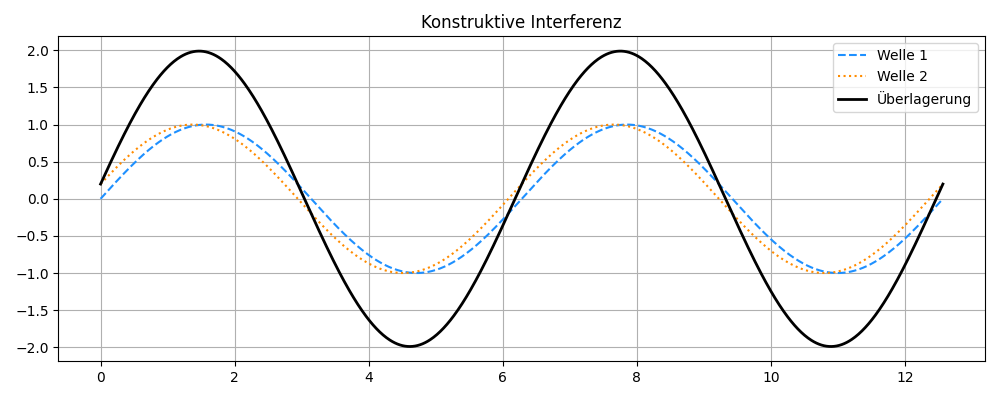
\includegraphics[width=1\linewidth]{images/physics/Interferenz_Konstruktiv.png}
    \caption{Konstruktive Interferenz zwischen zwei Wellen}
    \label{fig:Interferenz_Konstruktiv}
\end{figure}

\begin{figure}[H]
    \centering
    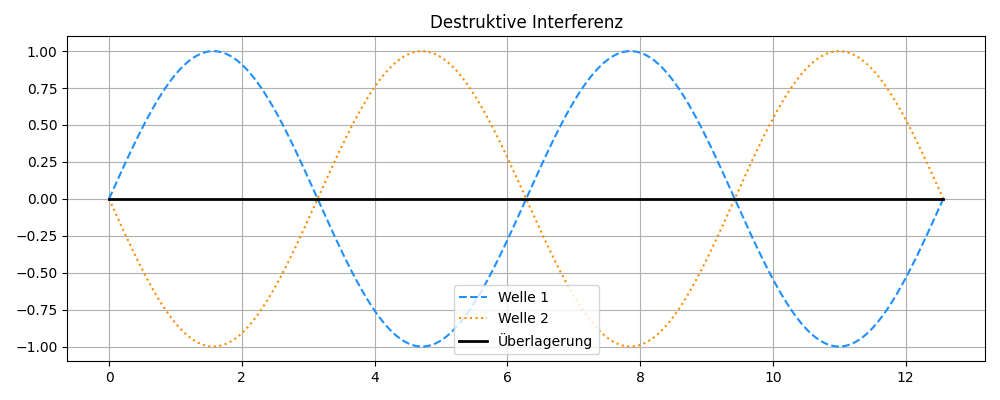
\includegraphics[width=1\linewidth]{images/physics/Interferenz_Destruktiv.png}
    \caption{Destruktive Interferenz zwischen zwei Wellen}
    \label{fig:Interferenz_Destruktiv}
\end{figure}

\subsection{Verschränkung }
\label{sec: Verschränkung}
Das Konzept der Verschränkung (engl. ``entanglement'') beschreibt gewissermaßen die Korrelation mehrerer Qubits miteinander, das heißt sie hängen in einem besonderen Maße zusammen. 

Für einen erleichterten Einstieg soll ein Beispiel anhand zweier gewöhnlicher Münzen gemacht werden. Werden zwei gewöhnliche Münzen geworfen, hat man vier mögliche Ausgänge für den Münzwurf, bei denen H für Kopf und T für Zahl stehen sollen: HH, HT, TH, TT. 

Alle Varianten der Ausgänge haben hierbei eine identische Wahrscheinlichkeit von 25\%. Sind diese zwei Münzen jedoch in einem verschränkten Zustand  $\frac{1}{\sqrt{2}} (\ket{HH} + \ket{TT})$, sind hierbei nur zwei Ausgänge möglich, die beide jeweils eine 50\%-Wahrscheinlichkeit haben, nämlich HH oder TT. \\
  
Diese Verschränkung ist unabhängig von der räumlichen Nähe der Münzen und kann über große Distanzen hinweg wirken. Weiß man das Ergebnis der einen Münze, so weiß man automatisch auch immer das Ergebnis der anderen Münze. Im Bereich der Quantenmechanik ist genau dies bezogen auf diverse Teilchen anstelle der Münzen möglich. 
Das Phänomen der Verschränkung ist jedoch ein reines Quantenphänomen, das keine Erklärung in der klassischen Physik besitzt. \\

Eine Vermutung über die Natur der Verschränkung besteht aus der sofortigen Informationsübertragung zweier Teilchen, die über die Schnelligkeit der Lichtgeschwindigkeit hinausgeht, was jedoch als widerlegt gilt. Stattdessen teilen Teilchen nicht-klassische Information während der Verschränkung, die im Messprozess beobachtet werden kann. \\ 

Eine weitere frühe Interpretation, bekannt unter dem Namen ``Hidden Variable Theory'', nahm an, dass Teilchen beim Erzeugen mit verbogenen Eigenschaften erschaffen werden, die Messergebnisse deterministisch bestimmen. Beispielsweise wäre hierfür der Zerfall eines Teilchens in zwei Teilchen. Auf Basis der Impulserhaltung kann man durch die Messung des Impuls des einen Teilchens auf den Impuls des anderen Teilchens schließen, da der Gesamtimpuls vorher bekannt ist. 
(vgl. \cite[Ch. 7]{hughes_quantum_2021})
% Quantum Computing for the Quantum Curious - Hughes et al. - 2021

Das Problem dieser Theorie findet sich jedoch in Bell's Theorem, das zeigt, dass wenn die Welt durch diese versteckten Variablen beschrieben wäre, gewisse mathematische Ungleichungen in Experimenten eingehalten werden müssten. 
Diese gelten als Einschränkungen für alle lokal-realistischen Theorien, d.h. Theorien, die annehmen, dass Lokalität und Realismus gelten. \\ 
Lokalität bedeutet hierbei, dass es keinen Einfluss gibt, der sich schneller als mit Lichtgeschwindigkeit ausbreiten kann. \\
Realismus bezieht sich auf die Annahme, dass physikalische Größen zu jedem Zeitpunkt definierte Werte besitzen, unabhängig davon, ob diese gemessen werden. \\

Die quantenmechanische Verschränkung erfüllt diese Annahmen durch die ``spukhafte Fernwirkung'' jedoch nicht, da es eine scheinbar unmittelbare Verbindung über sehr große Distanz hinweg gibt. Dem Lokalitätsprinzip entsprechend, könnten zwei Systeme sich nur dann beeinflussen, wenn sie einen Kontakt oder ein physikalisches Feld haben, das sie verbindet. Quantenobjekte haben jedoch durch die mangelnde Lokalität keine klassische Kausalität, sondern nur die Beobachtung, dass die Ergebnisse immer korrelieren, auch wenn sie räumlich weit voneinander getrennt sind.
\\ 

Da die Grenzen der Bell-Ungleichung also nicht auf gemessene Experimente zutreffen, kann keine lokal-realistische Theorie das quantenmechanische Phänomen der Verschränkung erklären. Die Resultate stimmen mit der Quantenmechanik überein, anstatt mit lokalen Theorien wie der Hidden Variable Theory. 
\\ 

Basierend hierauf ergibt sich das Dilemma, dass Realismus und Lokalität nicht beide gleichzeitig gelten können. Diese Schlussfolgerung führt jedoch zu tiefergehenden philosophischen Fragen über die Realität, die an dieser Stelle nicht weiter behandelt werden sollen. Unabhängig davon findet die Verschränkungen Anwendungen in moderner Quantentechnologie, wie in der Quantenkryptographie oder Quanten-Teleportation.  
(vgl. \cite[Ch. 2.11]{homeister_quantum_2022-1})
%% Quantum Computing verstehen: Grundlagen - Anwendungen - Perspektiven - Homeister - 2022
\\

Um ein Beispiel für die Quantenverschränkung in der Praxis zu machen, soll an dieser Stelle noch  die spontane parametrische Fluoreszenz (engl. ``spontaneous parametric down-conversion, SPDC'') genannt werden. Bei diesem Prozess trifft ein Photon aus einem Laser auf ein nichtlineares Kristallmaterial. Dadurch spaltet sich das Photon in zwei neue Photonen, wobei die Polarisation der neuen Photonen miteinander verschränkt sind, sodass man typischerweise folgenden Zustand erhält:

\[
\frac{1}{\sqrt{2}}  ( \ket{H}_A \ket{H}_B + \ket{V}_A \ket{V}_B )
\]

Misst man also die Polarisation des Photons A, kennt man ebenfalls die Polarisation des Photons B, jedoch ohne dass dies klassisch bereits festgelegt war.
(vgl. \cite[Ch. 7]{hughes_quantum_2021})
% Quantum Computing for the Quantum Curious - Hughes et al. - 2021


\section{Zwei-Niveau-Systeme}
\label{Zwei-Niveau-Systeme}

Zwei-Niveau-Systeme bilden das elementarste Modell der Quantenmechanik und sind gleichzeitig von grundlegender Bedeutung für die Quanteninformatik. Sie beschreiben physikalische Systeme, die sich ausschließlich in einem von zwei möglichen Energiezuständen befinden können oder in einer Überlagerung dieser beiden. Beispiele sind Elektronenspin-Zustände, Polarisationsrichtungen von Photonen oder vereinfachte atomare Übergänge.

Trotz ihrer mathematischen Einfachheit erlauben Zwei-Niveau-Systeme die Beschreibung zentraler quantenphysikalischer Phänomene: Superposition, Interferenz, Verschränkung und quantenmechanische Zeitentwicklung lassen sich bereits in diesem reduzierten Modell erfassen. In der Quanteninformatik entspricht ein solches Zwei-Niveau-System genau einem Qubit (vgl.\autocite[Kapitel 1.2]{nielsen_quantum_2010}).

In den folgenden Abschnitten werden wir die Zustände dieser Systeme formal beschreiben, deren Interpretation erarbeiten und zeigen, wie man sie sowohl algebraisch als auch geometrisch fassen kann. Ziel ist es, eine konzeptionelle Brücke zwischen den mathematischen Grundlagen aus \nameref{Mathematische Beschreibung von Qubits} und den algorithmischen Anwendungen in Kapitel \ref{qbits} zu schlagen.

\subsection{Darstellung von Zuständen: Bra-Ket-Notation}
\label{Darstellung von Zuständen: Bra-Ket-Notation}
Zur Darstellung von Zuständen in Zwei-Niveau-Systemen verwendet man die sogenannte Bra-Ket-Notation, die auf Paul Dirac zurückgeht. Zustände werden durch sogenannte Kets $\ket{\psi}$ dargestellt. Das sind Vektoren im komplexen Hilbertraum. Das adjungierte Objekt ist das Bra $\langle \psi|$, ein linearer Funktional, der jedem Vektor einen komplexen Skalar zuordnet.

Das Skalarprodukt zweier Zustände $\ket{\phi}$ und $\ket{\psi}$ wird in dieser Notation als $\langle \phi | \psi \rangle$ geschrieben. Es ist linear im zweiten und semilinear im ersten Argument und erfüllt die Bedingungen eines inneren Produkts.



Diese Trennung hilft, physikalische Prozesse wie Übergangsamplituden oder Projektionen formal und gedanklich zu strukturieren.

\paragraph{Dualraum und Funktionalinterpretation}

Formal lässt sich der Bra-Vektor $\langle \phi|$ als Element des sogenannten Dualraums $\mathcal{H}^*$ des Hilbertraums $\mathcal{H}$ auffassen. Dieser Dualraum besteht aus allen linearen Abbildungen von $\mathcal{H}$ in die komplexen Zahlen, also aus Funktionalen:

\[
\mathcal{H}^* = \{ f : \mathcal{H} \to \mathbb{C} \,|\, f \text{ linear} \}.
\]

Das Skalarprodukt $\langle \phi | \psi \rangle$ kann daher auch als die Anwendung eines solchen Funktionals $\langle \phi|$ auf einen Vektor $|\psi\rangle$ verstanden werden. Diese Interpretation betont die asymmetrische Rolle von Bra- und Ket-Vektoren in der Dirac-Notation und macht die mathematische Struktur explizit.

Die Bra-Ket-Notation erlaubt eine elegante Darstellung linearer Operatoren: Ein Projektionsoperator beispielsweise wird als $|\psi\rangle\langle\psi|$ geschrieben und projiziert auf den Zustand $|\psi\rangle$. Diese Notation ist nicht nur formal nützlich, sondern auch konzeptionell bedeutsam, um Zustände, Operatoren und Messprozesse mathematisch zu trennen (vgl. \cite[Kap.~3.2]{nolting_springer_2013}).

\subsection{Globale Phasen und der projektive Hilbertraum}
\label{subsec:Globale Phasen und der projektive Hilbertraum }

Ein zentrales Konzept in der Quantenmechanik ist die Äquivalenz von Zuständen, die sich nur durch einen globalen Phasenfaktor unterscheiden. Zwei Vektoren $|\psi\rangle$ und $e^{i\theta} |\psi\rangle$, wobei $\theta \in \mathbb{R}$, repräsentieren denselben physikalischen Zustand. Alle beobachtbaren Größen hängen nur von relativen Phasen ab.

Diese Eigenschaft motiviert die Einführung des projektiven Hilbertraums, der alle physikalisch äquivalenten Zustände zusammenfasst. Formal handelt es sich um die Quotientenmenge $\mathbb{P}(\mathcal{H}) = \mathcal{H} \setminus \{0\} \,/\, \sim$, wobei $|\psi\rangle \sim e^{i\theta}|\psi\rangle$ (vgl. \cite[Kap 2.1]{nielsen_quantum_2010}). Dies stellt sicher, dass nur physikalisch unterscheidbare Zustände getrennt behandelt werden.


\section{Quantenmessung }
\label{sec: Quantenmessung}
Im folgenden Kapitel wird die Messung eines quantenmechanischen Systems betrachtet. Es wird genauer auf Observablen und ihre Rolle in der Messung, den Effekt einer Messung auf das Quantensystem, den Zerfall der Wellenfunktion, den Nichtdeterminismus einer quantenmechanischen Messung und das Messergebnis eingegangen. 
\subsection{Grundlagen der Quantenmessung}
\label{subsec: Grundlagen der Quantenmessung}
Die Messung in der Quantenmechanik unterscheidet sich grundlegend von der Messung in der klassischen Physik, einerseits durch die Auffassung der Grundkonzepte der Quantenmechanik, andererseits durch die mathematische Beschreibung und Interpretation der Messergebnisse.
In der klassischen Welt wird das Verhalten eines Systems nicht durch das alleinige Beobachten des Systems beeinflusst; ein Ball beispielsweise wird sein Verhalten und seine Flugkurve nach einem Schuss nicht verändern, unabhängig davon, ob jemand dabei zusieht oder nicht. 

In der Quantenwelt hingegen sind die gemessenen Objekte (z.B. Photonen) winzig klein und die entsprechenden Messgeräte verhältnismäßig groß, sodass schon alleine deshalb die Messung zwangsläufig den Zustand eines Quantensystems beeinflussen wird. 

Dass eine Messung den Zustand des Quantensystems verändert und das Ergebnis dieser Messung zufällig ist, ist im Rahmen des zweiten Postulats der Quantenmechanik eine zentrale Annahme, die in diesem Kapitel weiter erörtert werden soll. Als Observablen- oder Messwertpostulat ist es das zentrale Postulat für die Messung im gegebenen Rahmen. 
\\

Das zweite Postulat besagt, dass eine Quantenmessung einer Projektion des Zustandes $\ket{\psi}$ auf eine Basis $\ket{|v_i|}$ entspricht. Mit der Wahrscheinlichkeit $|\braket{v_i|\psi}|^2$ erhalten wir das Ergebnis $v_i$. Das System befindet sich dann im Zustand $\ket{v_i}$. 
(vgl. \cite[Ch. 1.4.1]{lvovsky_quantum_2018}) 
% Lvovsky - Quantum Physics - 2018 - Kapitel 1.4.1 The Measurement Postulate
\newline Dieses Konzept wird auch 'projektive Messung' genannt, da die Messung des Zustandes auf einen Basiszustand projiziert wird, wobei die Begriffe der Projektion und der Basiszustände noch weiter erläutert werden sollen. 
\\

Ein Quantensystem wird innerhalb einer bestimmten Basis gemessen.Der Begriff 'Basiszustand' bezieht sich hierbei auf die möglichen Zustände eines Systems, die insgesamt die Basis bilden (beispielsweise $\ket{v_1}$ oder $\ket{v_2}$) und bei der Messungen angenommen werden können.
Beim Messen springt das System in einen der Basiszustände. 
Wird hierbei der Wert $v_i$ gemessen, so springt das System in den Zustand $\ket{v_i}$. Das Messergebnis ist also der Zustand $\ket{v_i}$. 
Dabei wird die Information, welche Zustände gemessen werden und welche entsprechenden Zahlenwerte ihnen zugeordnet werden, in einem 'Observable Operator' zusammengefasst. 

Dieser Observable Operator, der die Basis der Messungen beschreibt und die möglichen Werte der Messung enthält, kann folgendermaßen dargestellt werden: 
\\
\begin{equation}
\hat{V} = \sum_i v_i \, \ket{v_i}\bra{v_i}
\end{equation}
\\ 
Jeder Zustand $\ket{v_i}$ ist hierbei ein Eigenzustand dieses Operators. Der dazugehörige Eigenwert $v_i$ ist der Zahlenwert der Messung, den man bei der Messung des Zustandes erhält. 

Die Zuordnung eines Wertes ist für einige Messgrößen (bspw. der Ort eines Teilchens im Raum) natürlich, für andere (z.B. die Polarisation eines Photons) weniger. Trotzdem wird auch in weniger natürlichen Fällen  eine Zahl zugeordnet, so beispielsweise +1 für eine horizontale $\ket{H}$ und -1 für eine vertikale $\ket{V}$ Polarisation. 
\\

Eine Observable kann für jede messbare Größe (Ort, Energie, Puls, Spin, etc.) definiert werden. Eine Ausnahme bildet hierbei die Zeit, da diese in der Quantenmechanik nicht als Observable definiert und behandelt wird.
Daher gibt es keinen Zeit-Operator oder Eigenzustände der Zeit. Die Zeit dient lediglich als kontinuierliche Variable zur Beschreibung der Entwicklung des Quantensystems. 
(vgl. \cite[Ch. 1.9.1]{lvovsky_quantum_2018})
% Lvovsky - Quantum Physics - 2018 - Kapitel 1.9.1 Observable Operators
\\

Projektive Messungen werden also durch eine Observable M beschrieben. Seien die Eigenwerte m die möglichen Ergebnisse der Messung und $P_m$ die zugehörigen Projektoren, kann M geschrieben werden als:
\begin{equation}
    M = \sum_m mP_m
\end{equation}
Hierbei sind $P_m$ die orthogonalen Projektoren auf den Eigenraum von M. Jeder Projektor projiziert auf einen Unterraum des Hilbertraums, der zu einem bestimmten Eigenwert m gehört. Diese Formel bildet die verallgemeinerte Darstellung der zuvor genannten Formel zur Darstellung der Observablen. \\ 

Es gelten daraus folgende Grundregeln: 
\begin{enumerate}
\item Die Gesamtwahrscheinlichkeit aller Messungen (Projektoren) ergeben in Summe 1, d.h. sie decken den gesamten Zustandsraum ab. Jeder mögliche Zustand wird durch eine Kombination der Projektoren beschrieben und bildet in Summe den Einheitsoperator. \\
\item Die Wahrscheinlichkeit einer Messung m ergibt sich aus folgender Formel:
\begin{equation}
    p(m) = \langle \psi \mid P_m \mid \psi \rangle
\end{equation}
Hierbei ist p(m) die Wahrscheinlichkeit, dass die Messung des Systems im Zustand $\ket\psi$ das Ergebnis m ergibt. Das ist mathematisch das s.g. Bornsche Wahrscheinlichkeitsgesetz.
Es ist das Quadrat der Länge der Projektion von $\ket\psi$ auf den m-Unterraum. Es berechnet also die Länge der Projektion von $\ket\psi$ auf den Eigenraum von m. \\
\item Nach einer Messung mit Ergebnis m kollabiert der Zustand $\ket\psi$ in einen Zustand, der der Messung entspricht. Dies wird auch Projektionspostulat genannt. Die Projektion dieses Zustandes muss wieder normalisiert werden, um wieder einen Zustand mit der Norm 1 zu erhalten.
Da wiederholte Messungen jedoch im Bereich des Quantumcomputing geringe Relevanz hat, wird auf die wiederholte Messung nicht weiter eingegangen. \\ 
\end{enumerate}

In kurz greift man bei der Messung eines Zustandes $\ket\psi$ also nur den Teil aus dem gesamten Zustandsvektor heraus, den man misst. Es wird der Anteil extrahiert, der zugehörig zum gemessenen Eigenwert ist, also die Projektion $P_m \ket\psi$. Der Zustand wird bei der Messung also in seine Bestandteile entsprechend der verschiedenen Eigenräume zerlegt. Um hieraus wieder einen gültigen und normierten Zustand zu erhalten, muss dieser Vektor mit seiner eigenen Länge normiert werden. Da wir in diesem Kontext jedoch keine wiederholte Messung identischer Qubits betrachten, wird die Normierung an dieser Stelle nicht weiter berücksichtigt und es wird stattdessen auf wiederholte Messungen verwiesen. 
(vgl. \cite[Ch. 3.9]{kasirajan_fundamentals_2021})
%Fundamentals of Quantum Computing: Theory and Practice – Kasirajan (Kapitel zu Projective Measurements)
\\ 

Um ein Beispiel für den Messprozess und den Zerfall auf den Eigenzustand bei der projektiven Messung zu machen, soll ein Photon auf einen Polarizing Beam Splitter (PBS) treffen. Dieser lässt horizontal polarisiertes Licht passieren, aber reflektiert vertikal polarisiertes Licht.
Betrachtet man einen Lichtstrahl aus der klassischen Physik, würde man erwarten, dass dieser sich teilt - ein Teil des Lichtes würde reflektiert werden, ein anderer Teil würde passieren. Ein Photon als kleinster Teil des Lichts kann jedoch nicht weiter geteilt werden.
Dementsprechend ist das Ergebnis zufällig: das Photon wird mit einer gewissen Wahrscheinlichkeit passieren oder reflektiert werden. Das Photon entscheidet sich bei der Messung, ob es horizontal oder vertikal polarisiert sein wird und springt bei der Messung in den gewählten Zustand. \\ \\
Man könnte auch sagen durch die Messung wird der Superpositionszustand auf einen der möglichen Eigenzustände reduziert. Die Superposition selbst liegt nicht im Eigenraum, sondern ist eine Überlagerung der Zustände aus den Eigenräumen, wobei ``horizontal'' und ``vertikal'' im Eigenraum mit ihrem jeweiligen Eigenwert liegen. Hierbei zerfällt der Ursprungszustand, sodass dies bei folgenden PBS nicht erneut vonstatten gehen könnte - das Photon wird den hierbei gewählten Zustand beibehalten.
Es gibt ab diesem Punkt keine weiteren zufälligen Zustandsänderungen. 
(vgl. \cite[Ch. 1.4.1]{lvovsky_quantum_2018})
% Quantum Physics – Lvovsky – 2018 (Kapitel 1.4.1 The Measurement Postulate)

\subsection{Nichtdeterminismus}
\label{subsec: Nichtdeterminismus}
Das oben beschrieben Phänomen der zufälligen Messung ist auf den Nichtdeterminismus der Quantenmessung zurückzuführen. Das bedeutet, dass das Ergebnis der Messung zufällig ist. Man erhält den Wert $\ket v_i$ mit einer gewissen Wahrscheinlichkeit.
Je besser der Zustand $\ket \psi$ zu einem Messzustand $\ket v_i$ passt, desto wahrscheinlicher ist das Ergebnis $v_i$. 
\\

Mit Hilfe des Observable Operators können Werte der klassischen Statistik berechnet werden, so der Erwartungswert, die Varianz bzw. die Unschärfe der Messung (Standardabweichung). 
Klassisch statistische Kennzahlen lassen sich mit klassischen Operationen berechnen. Entsprechend ist die statistische Verteilung der Messergebnisse leicht zu berechnen. 
\\ 

Um hierbei auf das Beispiel der Photonen zurückzukommen, führen wir ein, dass die horizontale Polarisierung des Photons dem Wert +1 zugeordnet wird, die vertikale Polarisierung dem Wert -1.
Ein diagonal polarisiertes Photon (45°) hat entsprechend eine 50\% Chance den PBS zu passieren (+1) oder reflektiert zu werden (-1). Bei der wiederholten Messung dieses Prozesses, ist der Mittelwert 0, da sich beide Superpositionen ausgleichen.
Die Varianz entspricht einem Wert von 1, da die Messung immer um +1 oder -1 vom Mittelwert (0) abweicht. 
\\

In der klassischen Physik sind solche Messungen deterministisch vorhersehbar. Für einzelne Photonen gibt es den Zufall, für eine Vielzahl von Photonen als Licht gibt es jedoch feste Erwartungen und Regeln.
Entsprechend ist es auch im Quantensystem. Mit einer Vielzahl an Photonen wird die relative Unsicherheit sehr klein und das Verhalten erscheint klassisch und stabil, obwohl die Photonen im Kleinen in Form der Einzelphotonen vom Zufall beherrscht sind.
Die Quantenfluktuationen verschwindend relativ gesehen also im großen Maßstab durch die wiederholte Messung und eine klare Wahrscheinlichkeitsverteilung.
(vgl. \cite[Ch. 1.9.2]{kasirajan_fundamentals_2021})
% Quantum Physics – Lyvovsky – 2018 (Kapitel 1.9.2 Observable Operators)
\\ 

Erwähnenswert im Rahmen der Messung ist weiterhin das 'Heisenbergsche Unschärfeprinzip'. In der klassischen Physik ist eine Unsicherheit im Rahmen der Messung Folge eines ungenauen Messapparates, die durch eine Verbesserung des Apparates selbst verringert werden kann. 

Dies gilt jedoch im Kontext der Quantenmechanik nicht. Hierbei kann ein Apparat präzise auf die Messung eines Observablen abgestimmt sein, jedoch bei der Messung einer anderen Observablen durchweg schlecht abschneiden. 

Möchte man zwei Größen gleichzeitig messen, beispielsweise Ort und Energie oder auch verschiedene Spins, so kann das möglich sein. Hierzu müssen jedoch zwei Observablen kommutieren, d.h. mathematisch verträglich sein, um gleichzeitig messbar sein zu können. 
Ist dies der Fall, gibt es eine bestimmte Basis von Zuständen (Eigenbasis), in der beide Observablen gleichzeitig genau bestimmt werden können. Das System in diesem Zustand verändert seinen Zustand nicht, wenn beide Größen nacheinander gemessen werden, d.h. die Observablen sind kompatibel. 

Wenn die Observablen jedoch nicht kommutieren, so gibt es keinen Zustand, bei dem man beide Größen gleichzeitig exakt wissen kann. Misst man hierbei A, wird das Ergebnis von B zufällig sein, da die Messung von B durch die Information über A gestört ist.
Das heißt bestimmte Paare von Größen können nicht gleichzeitig beliebig genau gemessen werden. 
Zwei Größen, die nicht kommutieren, sind z.B. Ort und Impuls eines Teilchens. Je genauer man den Ort kennt, desto ungenauer lässt sich der Impuls messen und umgekehrt. 
(vgl. \cite[Ch. 1.9.3]{kasirajan_fundamentals_2021})
% Quantum Physics – Lyvovsky – 2018 (Kapitel 1.9.3 Uncertainty Principle)

\subsection{Messprozess}
\label{subsec: Messprozess}

Ein Prozess, der im Rahmen der Messung bereits mehrfach erwähnt, jedoch bisweilen noch nicht konkret benannt wurde, ist der Kollaps der Wellenfunktion. Dieser Prozess ist zentral für die Messung. 
Unter dem Kollaps der Wellenfunktion versteht man den Vorgang, bei dem der Zustand eines Quantensystems auf einen Basiszustand 'springt', das heißt der Zustand des Systems kollabiert auf einen der möglichen Messzustände. Die Wahrscheinlichkeit für den Wert, den man beim Kollaps erhält, ist durch die bereits genannte Bornsche Regel beschrieben. \\
Dies zeigt die Annahme der Quantenmechanik des Nichtdeterminismus, dass der Zufall grundlegend ist. Selbst mit perfekten Geräten kann der Zustand entsprechend nicht exakt vorhergesagt werden. 
(vgl. \cite[Ch. 1.4.1]{lvovsky_quantum_2018})
% Quantum Physics – Lyvovsky – 2018 (Kapitel 1.4.1 The Measurement Postulate)
\\

Ein Quantenzustand ist also nur in abgeschottetem Zustand stabil. Um aus Perspektive der Außenwelt etwas über den Zustand des Systems zu erfahren, ist jedoch eine Messung nötig, wobei der genaue Zustand nicht ermittelt werden kann.
Die Superposition selbst wird durch die Messung zerstört und ein klassischer Zustand wird angenommen und beobachtet. Da diese Messung für verschiedene Basen möglich ist, jedoch nur der Zustand bzgl. einer Basis gemessen werden kann, ist die folgende Messung durch den Zerfall nicht weiter möglich.
Da die Messung nicht rückgängig gemacht werden kann, kann durch den Kollaps der Wellenfunktion dieselbe Messung im gleichen System nicht wiederholt werden.
(vgl. \cite[Ch. 2.8]{homeister_quantum_2022})
% Quantum Computing verstehen: Grundlagen – Anwendungen – Perspektiven – Homeister – 2022 (Kapitel 2.8 Das Messen von Quantenregistern)
\\

Aus diesem Phänomen ergibt sich auch das No-Cloning-Theorem. Da das System selbst bei der Messung zerstört wird, kann das Qubit nicht erneut gemessen werden. Die Superposition selbst ist für dasselbe Qubit nicht mehr vorhanden. Die Messung kann entsprechend nur für ein gleiches Qubit wiederholt werden.
Folglich dieser Logik kann ein Qubit in einem unbekannten Zustand nicht kopiert werden. Dies hat wichtige Konsequenzen für die praktische Anwendung, da simple Kopien, wie sie auf klassischen Computern möglich sind, durch die zuvor notwendige Messung der bestehenden Zustände nicht ohne Weiteres auf quantenbasierten Systemen ermöglicht werden.
(vgl. \cite[Ch. 4.4]{hughes_quantum_2021})
% Quantum Computing for the Quantum Curious – Hughes et al. – 2021 – s. 36

\subsection{Mathematische Struktur von Messungen}
\label{subsec: Mathematische Struktur von Messungen}
Statt auf technische Realisierungen einzugehen, liegt der Fokus dieses Abschnitts auf der abstrakten Beschreibung von Messprozessen. Eine Messung in einem Zwei-Niveau-System wird durch einen Satz orthonormaler Projektionsoperatoren beschrieben, die auf den Zustandsraum wirken. Das Messergebnis ist mit der Wahrscheinlichkeit $|\langle\phi|\psi\rangle|^2$ verbunden, wenn $\ket{\phi}$ der gemessene Eigenzustand ist (siehe \cite[Kap 2.2] {nielsen_quantum_2010}).

Messprozesse führen im Allgemeinen zu einem Kollaps des Zustandsvektors auf den gemessenen Eigenzustand. Dieser Übergang lässt sich mathematisch als nicht-unitäre Projektion formulieren. Die Kombination aus linearem Zustand, unitärer Entwicklung und projektiver Messung bildet das Grundgerüst der quantenmechanischen Theorie.


Zwei-Niveau-Systeme sind das einfachste, aber zugleich zentrale Modell der Quantenmechanik. Ihre mathematische Beschreibung durch Vektoren im Hilbertraum, die Interpretation über Bra-Ket-Notation, die Berücksichtigung globaler Phasen und ihre geometrische Darstellung auf der Bloch-Kugel liefern ein vollständiges und vielseitiges Bild (siehe \cite[Kap 3.5] {greiner_quantenmechanik_nodate}).

Diese Konzepte sind nicht nur grundlegend für das Verständnis der Quantenmechanik, sondern auch zentrale Bausteine für die Beschreibung und Entwicklung von Quantenalgorithmen und Quantenhardware.



\section{Mathematische Beschreibung von Qubits}
\label{Mathematische Beschreibung von Qubits}

Die mathematische Beschreibung eines Qubits bildet das Fundament der quantenmechanischen Informationsverarbeitung. Während ein klassisches Bit stets in genau einem von zwei diskreten Zuständen vorliegt, kann ein Qubit eine lineare Überlagerung dieser beiden Zustände einnehmen. Diese Eigenschaft, die als Superposition bezeichnet wird, verlangt nach einer mathematischen Struktur, die solche Kombinationen zulässt und konsistent interpretierbar macht.

\subsection{Der Hilbertraum des Qubits}
\label{subsec: Der Hilbertraum des Qubits}

Ein Qubit wird als Vektor in einem zweidimensionalen komplexen Vektorraum beschrieben, der mit einem Skalarprodukt ausgestattet ist. Dieser Raum wird als Hilbertraum bezeichnet und durch \( \mathcal{H} = \mathbb{C}^2 \) dargestellt. Er enthält alle linearen Kombinationen zweier orthonormaler Basisvektoren, die mit \( |0\rangle \) und \( |1\rangle \) bezeichnet werden. Diese sogenannten Basiszustände werden üblicherweise in Form von Spaltenvektoren geschrieben:

\[
\ket{0} = \begin{pmatrix} 1 \\ 0 \end{pmatrix}, \quad \ket{1} = \begin{pmatrix} 0 \\ 1 \end{pmatrix}
\]

Ein vollständiges System orthonormaler Basiszustände bildet eine Basis des Hilbertraums. Jeder beliebige Zustand in \( \mathcal{H} \) kann als Linearkombination dieser Basiszustände dargestellt werden. Für endliche Quantensysteme ist \( \mathcal{H} \) endlichdimensional, typischerweise mit \( \dim \mathcal{H} = 2^n \) für ein System aus \( n \) Qubits. In vielen physikalischen Anwendungen, etwa in der Quantenfeldtheorie oder bei kontinuierlichen Freiheitsgraden, ist \( \mathcal{H} \) jedoch unendlichdimensional. In solchen Fällen gewinnt die mathematische Struktur des Hilbertraums an Komplexität.

Um physikalisch sinnvoll zu sein, fordert man zusätzlich zur Vollständigkeit oft auch die Separabilität des Hilbertraums. Ein separabler Hilbertraum enthält eine abzählbare dichte Teilmenge, wodurch gewährleistet ist, dass der Raum mithilfe einer zählbaren Basis „erreichbar“ ist. Diese Eigenschaft ist für die mathematische und physikalische Handhabbarkeit entscheidend (\cite[Kap. 2] {nolting_springer_2013}). 

\subsection{Mathematische Struktur und Operatoren im Hilbertraum}
\label{subsec:Mathematische Struktur und Operatoren im Hilbertraum}

Ein Hilbertraum ist ein Vektorraum mit einem Skalarprodukt, der vollständig in Bezug auf die durch das Skalarprodukt induzierte Norm ist. Vollständigkeit bedeutet, dass jede sogenannte Cauchy-Folge von Vektoren in diesem Raum gegen einen Vektor desselben Raumes konvergiert (\cite[Kap.2]{nolting_springer_2013}).

Eine Cauchy-Folge \( \{ |\psi_n\rangle \} \) ist eine Folge von Vektoren, bei der der Abstand zwischen den Folgengliedern mit wachsendem Index beliebig klein wird. Formal gilt: Zu jedem noch so kleinen positiven \( \varepsilon \) existiert ein Index \( N \), sodass für alle \( m,n > N \) die folgende Bedingung erfüllt ist:

\[
\| \ket{\psi_n}  - \ket{\psi_m}  \| < \varepsilon
\]

Die Vollständigkeit besagt, dass diese Folge gegen einen Grenzwert \( \ket{\psi} \) innerhalb des Raumes konvergiert. Dies stellt sicher, dass der Raum bezüglich der durch das Skalarprodukt definierten Metrik keine „Lücken“ enthält. Anschaulich bedeutet das: Jeder Zustand, der durch eine Folge angenähert werden kann, gehört auch tatsächlich zum Raum.

Das durch das Skalarprodukt induzierte Normkonzept ermöglicht es, eine Metrik und damit eine topologische Struktur auf dem Raum zu definieren. Dies erlaubt es, Begriffe wie Konvergenz, Stetigkeit und Orthogonalität mathematisch präzise zu fassen. Diese Konzepte bilden die Grundlage für eine konsistente Beschreibung quantenmechanischer Zustände (vgl. \cite[Kapitel V]{werner_funktionalanalysis_2002}).

Zudem ist der Hilbertraum die natürliche Umgebung für sogenannte unitäre Operatoren. Ein Operator \( U \) auf einem Hilbertraum ist genau dann unitär, wenn er die Struktur des Raumes erhält, das heißt:

\[
U^\dagger U = I
\]

Solche Operatoren spielen eine zentrale Rolle in der Quanteninformatik. Sie modellieren reversible Zeitentwicklungen und logische Operationen auf Qubits.

Ein praktisches Anwendungsbeispiel für unitäre Operatoren ist die gezielte Erzeugung von Superpositionen durch sogenannte Quantenlogikgatter. Bereits das Hadamard-Gatter ermöglicht es, aus einem Basiszustand einen Zustand mit gleichverteilter Wahrscheinlichkeit über mehreren Basisvektoren zu erzeugen. Solche Superpositionen sind nicht nur ein theoretisches Konstrukt, sondern Grundlage für Effekte wie Quantenparallelität und Interferenz. Diese wiederum spielen in komplexeren Verfahren wie der Quanten-Fourier-Transformation eine zentrale Rolle, die in Kapitel~4 behandelt wird. Die Fähigkeit, Zustände durch unitäre Operatoren gezielt zu transformieren, bildet somit das Fundament für die dynamische Entwicklung quantenmechanischer Systeme.

Weitere Beispiele für unitäre Operatoren und ihre Funktion in Quantenalgorithmen werden in Kapitel \ref{qbits} behandelt.



Die mathematische Struktur des Hilbertraums erlaubt es, Qubit-Zustände sowohl algebraisch als auch geometrisch zu beschreiben. Die Bra-Ket-Notation stellt eine kompakte Form dar, um Zustände und ihre Transformationen mathematisch zu erfassen. 

Ein weiteres zentrales Konzept ist die Äquivalenz unter einer globalen Phase. Zwei Zustände, die sich lediglich durch einen komplexen Phasenfaktor unterscheiden, sind physikalisch nicht unterscheidbar. Diese Eigenschaft führt zur Beschreibung der Zustände im sogenannten projektiven Hilbertraum. Die geometrische Konsequenz dieser Beschreibung ist die Bloch-Kugel, auf der alle reinen Qubit-Zustände als Punkte auf einer Kugeloberfläche dargestellt werden können.


Der Qubit-Zustand ist ein normierter Vektor in einem komplexen Hilbertraum. Die mathematische Struktur dieses Raums erlaubt die präzise Definition von Superposition, Normierung, Skalarprodukt, Phasenäquivalenz und linearen Transformationen. Die Vollständigkeit und Separabilität des Hilbertraums stellen sicher, dass auch Grenzwerte und stetige Prozesse sinnvoll beschrieben werden können. Die Möglichkeit unitärer Operatoren ist eine direkte Konsequenz der Struktur des Hilbertraums und erlaubt die Darstellung quantenmechanischer Zeitentwicklungen und Quantenlogik. Die Konzepte der Basiswahl und Dimensionsabhängigkeit verknüpfen die abstrakte Struktur des Hilbertraums mit der physikalischen Realität eines Quantensystems. Diese Grundlagen sind entscheidend für die Beschreibung von Messprozessen, physikalischen Realisierungen und logischen Operationen in der Quanteninformatik.

\section{Physikalische Realisierung von Qubits }
\label{sec: Physikalische Realisierung}
\subsection{Anforderungen an physikalische Systeme }
\label{subsec: Anforderungen (Allgemein, Divincenzo-Kriterien, Dekohärenz)}
\subsubsection{Allgemeine Voraussetzungen}

\textbf{Robuste Darstellung von Quanteninformation:}

Damit ein physikalisches System für die Realisierung von Qubits infrage kommt, müssen verschiedene Voraussetzungen erfüllt sein. Im ersten Teil dieses Kapitels werden diese Voraussetzungen erläutert, während der zweite Teil eine Einführung in geeignete physikalische Systeme gibt.\\

Für praktische Quantenberechnungen ist es entscheidend, dass das System nur eine \textbf{endliche Menge zugänglicher Zustände} besitzt. Systeme mit einem kontinuierlichen Zustandsraum, wie etwa die Position eines Teilchens auf einer Linie, sind ungeeignet. 


Auch wenn solche Systeme in der Theorie unendlich viele Zustände unterscheiden könnten (und damit unbegrenzt Information speichern würden), ist dies in der Praxis unrealistisch. Denn reale physikalische Systeme sind störanfällig, da das sogenannte Rauschen die Zahl unterscheidbarer Zustände und die damit zusammenhängende Informationskapazität begrenzt. \\

Ein weiterer wichtiger Aspekt ist die \textbf{Symmetrie} des Systems. Symmetrisch beschränkte Zustandsräume wie der zweidimensionale Raum eines Spin-1/2-Teilchens mit den Zuständen $\ket{\uparrow}$ und $\ket{\downarrow}$ – helfen, die Stabilität der Quanteninformation zu sichern. Solche Systeme sind weniger anfällig für Störungen von außen und daher besser gegen Dekohärenz geschützt. Die Wahl eines symmetrischen, wohldefinierten Zustandsraums kann somit entscheidend zur Fehlerresistenz eines Qubits beitragen.


Demgegenüber können \textbf{ungeeignete physikalische Repräsentationen} schnell zur Dekohärenz führen. Ein Beispiel ist ein Teilchen in einem flachen Potentialtopf, das nur gerade tief genug ist, um zwei gebundene Zustände zu enthalten. Solch ein System könnte zwar theoretisch als Qubit verwendet werden – es besteht jedoch die Gefahr, dass das Teilchen durch äußere Einflüsse in den ungebundenen Bereich des Kontinuums übergeht. Dadurch würde der Zustand aus dem definierten Zustandsraum „herausspringen“, was zur Zerstörung der Superposition und damit zu Informationsverlust führt.\\

Grundsätzlich muss ein System in der Lage sein, Quanteninformation zuverlässig in physikalischen Zuständen (Qubits) zu speichern, sodass sie ihre charakteristischen Quanteneigenschaften wie Superposition und Verschränkung ausreichend lange beibehalten. 


Zur quantitativen Bewertung der Qualität eines Qubits betrachtet man daher die Lebensdauer seiner Zustände. Die sogenannte \textbf{$T_2$}-Zeit gibt an, wie lange eine Superposition (z.B. 
$\ket{0} + \ket{1}$) stabil bleibt – sie ist ein Maß für die Kohärenzzeit. \\
Im Vergleich dazu beschreibt die \textbf{$T_1$-}Zeit die Lebensdauer des angeregten klassischen Zustands $\ket{1}$ und ist in vielen Systemen deutlich länger als $T_2$. Beide Größen sind zentrale Kenngrößen für die Praxistauglichkeit einer Qubit-Implementierung.\\

Die Dauer sinnvoller Quantenberechnungen wird vor allem durch das Verhältnis von Kohärenzzeit (\(\tau_Q\)) zu Operationszeit (\(\tau_{op}\)) bestimmt. Dieses Verhältnis 
\(\lambda = \frac{\tau_{op}}{\tau_Q}\) zeigt, wie viele Rechenschritte möglich sind, bevor Dekohärenz einsetzt. Sowohl \(\tau_Q\) als auch \(\tau_{op}\) hängen stark von der Kopplung des Systems zur Umgebung ab, wodurch \(\lambda\) je nach physikalischem System stark variieren kann. 


Eine Übersicht der verschiedenen Kohärenzzeiten für unterschiedliche physikalische Systeme wird in Tabelle 1.1 aufgezeigt. Grobe Schätzwerte für Dekohärenzzeiten \(\tau_Q\), Operationszeiten \(\tau_{op}\) und die maximale Anzahl möglicher Operationen  $n_{\text{op}} = \frac{T_Q}{T_{\text{op}}}$  für verschiedene physikalische Realisierungen von Qubits. Trotz der Vielzahl an Einträgen basieren sie auf nur drei grundlegenden Qubit-Typen: Spin, Ladung und Photon. 


\begin{table}[h]
    \centering
    \begin{tabular}{|l|c|c|c|}
        \hline
        \textbf{System} & $\tau_Q$ & $\tau_{op}$ & $n_{op} = \lambda^{-1}$ \\
        \hline
        Kernspin& $10^{-2} - 10^8$ & $10^{-3} - 10^{-6}$ & $10^5 - 10^{14}$ \\
        Elektronenspin& $10^{-3}$ & $10^{-7}$ & $10^4$ \\
        Ionenfalle& $10^{-1}$ & $10^{-14}$ & $10^{13}$ \\
        Elektron - Galliumarsenid (GaAs)& $10^{-10}$ & $10^{-13}$ & $10^3$ \\
        Optischer Resonator& $10^{-5}$ & $10^{-4}$ & $10^4$ \\
        Mikrowellenresonator& $10^{0}$ & $10^{-4}$ & $10^4$ \\
        \hline
    \end{tabular}
    \caption{Grobe Schätzwerte für Dekohärenzzeiten}
    \label{tab:quantum_systems}
\end{table}
(basierend auf \cite[Ch. 7.1]{nielsen_quantum_2010})
%S. 278
\\
 Eine weitere Voraussetzung für die physikalische Realisierung von Qubits ist die Möglichkeit, eine Vielzahl kontrollierter Quantenoperationen durchzuführen, die jede beliebige quantenlogische Berechnung ermöglichen (Universalität).
 
 
 Weiterhin  muss das System zu Beginn der Berechnung in einen gut bekannten Ausgangszustand gebracht werden können – typischerweise alle Qubits im Zustand |0⟩. Nach der Berechnung muss der finale Zustand des Systems dann zuverlässig gemessen werden können, um ein klassisches Ergebnis zu erhalten. 
 

Die große Herausforderung dabei ist, dass diese Voraussetzungen häufig nur teilweise erfüllt werden können, da sie gegensätzlich sind: ein Quantencomputer muss gut isoliert sein, um die Quanteneigenschaften beizubehalten; aber gleichzeitig müssen die Qubits so zugänglich sein, dass man sie für eine Computation manipulieren kann und die Ergebnisse messen kann. 


Als Beispiel kann ein Münzwurf betrachtet werden: Eine Münze repräsentiert während eines Münzwurfes ein gutes Bit, weil sie zwei States hat (Kopf und Zahl), aber ein schlechtes Qubit, weil sie nicht lange im Status der Superposition bleibt. Ein einzelner Nuklear-Spin hingegen wäre ein sehr gutes Qubit, weil eine Superposition lange beibehalten werden kann, jedoch ist die Messbarkeit sehr schwierig, was es wiederum zu einem schlechten Quantencomputer macht. (vgl. \cite[Ch. 7.1]{nielsen_quantum_2010})


\subsubsection{DiVincenzo Kriterien}

Die DiVincenzo-Kriterien, benannt nach dem Physiker David Divincenzo, beschreiben fünf grundlegende Anforderungen, die ein Quantencomputer erfüllen muss, um prinzipiell funktionsfähig und skalierbar zu sein. Sie dienen als Leitfaden für die Entwicklung praktischer Quanteninformationsverarbeitungssysteme. Nachfolgend wird eine Aufzählung dieser Kriterien sowie eine kurze Erklärung gegeben. \\

\textbf{1. Präzise definierter und skalierbarer Zustandsraum (Hilbertraum): Qubits als klar identifizierbare, kombinierbare Subsysteme} 

Damit Quantenalgorithmen ihr volles Potenzial entfalten können, sind oft Millionen Qubits erforderlich. Die Herausforderung liegt hierbei nicht nur in der Herstellung dieser großen Anzahl an Qubits, sondern auch in der kontrollierten Ansteuerung dieser ohne Energieverluste oder Dekohärenz.


Die relevanten Freiheitsgrade eines physikalischen Systems müssen als wohldefinierte Dimensionen im Hilbertraum abgebildet sein. Dieser Zustandsraum muss präzise bestimmbar und in ein direktes Produkt kleinerer Teilsysteme – den einzelnen Qubits – zerlegbar sein. Nur so lassen sich Qubits eindeutig identifizieren und kombinieren.


Zudem ist eine möglichst gute Isolation von der Umgebung notwendig, um störende Wechselwirkungen zu vermeiden. Entscheidend ist auch, dass der Zustandsraum mit der Anzahl der Qubits exponentiell wächst – nur dann entsteht ein echter Vorteil gegenüber klassischen Computern (vgl. \cite[Ch. 18]{lapierre_introduction_2021}).
 \\

\textbf{{2. Möglichkeit eines Startzustands} }

Eine Quantenberechnung muss von einem Startzustand ausgehen, der kontrolliert reproduzierbar ist. Typischerweise ist dies der Grundzustand \(\left| 0\right\rangle\) \(\left| 0\right\rangle\) \(\left| 0\right\rangle\) ... \(\left| 0\right\rangle\)〉, der durch eine Kühlung des Quantensystems erreicht wird.  Der Aufwand dafür ist abhängig vom jeweiligen System: beispielsweise bei Atomfallen wird das System auf Nano-Kelvin heruntergekühlt. 

Es existieren zudem auch weitere Techniken wie "optical pumping"; diese werden hier jedoch nicht weiter betrachtet (vgl. \cite[Ch. 18]{lapierre_introduction_2021}). \\


\textbf{3. Isolation und Erhaltung der Kohärenz} 

Ein zentrales Problem für Quantencomputer ist die Dekohärenz, die durch unerwünschte Wechselwirkungen des Systems mit der Umgebung entsteht: das System wird mit äußeren Freiheitsgraden verschränkt und verliert dadurch seine quantenmechanischen Eigenschaften, was zu Fehlern und gemischten Zuständen führt. Die Fehlertoleranz in Quantensystemen ist sehr gering (derzeit praktikabel nur bei $\varepsilon < 10^{-6}$), weshalb eine starke Isolation und eine möglichst lange Kohärenzzeit entscheidend sind. Mehr Informationen zur Dekohärenz werden im nächsten Unterpunkt gegeben. \\

 
\textbf{4. Kontrollierbare Transformationen des Zustands (Quantengatter)}

Es ist essenziell, selektiv steuerbare Operationen an Qubits durchführen zu können, die keine ungewollten Nebenwirkungen erzeugen. Solche Transformationen werden meist durch zeitabhängige Hamiltonian-Änderungen realisiert, beispielsweise über Laserstrahlen, Magnetfelder etc. \\


5. \textbf{Messung einzelner Qubits im Eigenbasiszustand} 
Für die Messung einzelner Qubits ist eine sogenannte "starke Messung" notwendig, die eine eindeutige Projektion des Zustands auf einen Basiszustand (z.B.  \(\left| 0\right\rangle\)oder \(\left| 1 \right\rangle\) ) ermöglicht. Eine "schwache Messung" hingegen, die nur Wahrscheinlichkeiten liefert, reicht nicht aus (vgl. \cite{divincenzo_topics_nodate}).
 
\subsubsection{Einführung in Dekohärenz }

\textbf{Dekohärenz als zentrales Problem}: 

Damit ein Quantencomputer zuverlässig funktionieren kann, müssen sorgfältig kontrollierte Bedingungen herrschen, die die Transformationen im Inneren des Computers nicht stören. Um als Quantencomputer zu fungieren, darf ein physikalisches System keine weiteren physikalischen Interaktionen haben, die nicht unter der Kontrolle des Programms sind. 


Der Begriff Dekohärenz beschreibt den Verlust von Quanteneigenschaften wie Superposition und Verschränkung durch ungewollte Wechselwirkungen mit der Umgebung, aber auch Störungen durch Interaktionen direkt innerhalb des Systems, zwischen den für die Berechnungen relevanten Merkmale der Qubits und den irrelevanten Aspekten. 


Auch wenn derartige Wechselwirkungen für herkömmliche, "klassische" Computer komplett irrelevant sind, können diese Interaktionen starke Auswirkungen auf die Operationen eines Quantencomputers haben (vgl. \cite[Ch. 1]{mermin_quantum_2012}).

\\
\textbf{Ursachen und Folgen von Dekohärenz}

Folgende Aspekte können die Ursache von Dekohärenz sein:


\begin{itemize}
    \item Thermische Fluktuationen
    \item Elektromagnetische Störungen
    \item Imperfekte Quanten-Gates (z.B. durch fehlerhafte Pulssteuerung)
    \item Wechselwirkungen mit der Umgebung (z.B. Vakuumfluktuationen, Gittervibrationen)
    \item Wechselwirkungen mit benachbarten Qubits (cross-talk)
\end{itemize}

(vgl. \cite[Ch. 1]{mermin_quantum_2012})
\\

Die Folgen der Dekohärenz sind, dass sich der Zustand eines Qubits ungewollt umdrehen kann, also von |0⟩ nach |1⟩ wechselt oder umgekehrt. Außerdem können durch Fehler die besonderen Quanteneigenschaften wie Superposition und Verschränkung verloren gehen. Dadurch wird die Leistungsfähigkeit von Quantenalgorithmen stark eingeschränkt und es wird schwieriger, größere und komplexere Berechnungen zuverlässig durchzuführen (vgl. \cite[Ch. 7]{nielsen_quantum_2010}).\\

%Fraunhofer Quantum computing compact training program 2025, S. 58 


\textbf{Lösungsansätze }

Um Dekohärenz so gut wie möglich zu vermeiden, werden Quanteninformationen bevorzugt in einer kleinen Anzahl von Zuständen eines atomaren Systems kodiert. In diesen sind die Abstände der diskreten Energieniveaus deutlich größer als in makroskopischen Systemen, wodurch eine  Isolation auf atomarer Ebene einfacher zu erreichen ist. Das bedeutet, dass im Vergleich ein deutlich größerer Einfluss auf ein Atom ausgewirkt werden muss, um dieses aus dem Grundzustand zu bewegen. Zusätzlich spielen interne Wechselwirkungen bei atomaren Systemen keine Rolle, da sie entweder nicht existieren, oder sehr hohe Energien erforderlich sind, um sie zu aktivieren.
Makroskopische Systeme hingegen könnten kaum gegen Umwelteinflüsse (und ihre eigenen irrelevanten internen Eigenschaften) isoliert werden. Die einzigen Interaktionen mit den Quantensystemen dürfen kontrollierte Interaktionen sein, die mit dem Computingprozess selbst zusammenhängen. \\

Die gute Nachricht ist, dass eine Fehlerkorrektur auch beim Quantencomputing prinzipiell möglich ist, solange die Einflüsse der Umwelt ausreichend niedrig sind. Das besagt das sogenannte "Treshold Theorem". Während eine Fehlerkorrektur bei klassischen Computern Routine ist, gestaltet sich der Prozess im Quantencomputing schwieriger: weder der ursprüngliche noch der fehlerhafte Zustand der Qbits ist dabei bekannt (vgl. \cite[Ch. 1]{mermin_quantum_2012}). 
Weitere Informationen zur Fehlerkorrektur im Kapitel \ref{error_correction}. \\

\subsection{Supraleitende Qubits }
\label{subsec: Supraleitende Qubits}

Supraleitende Qubits sind über den kollektiven Zustand einer großen Anzahl an Elektronen codiert.
Sie gelten als vielversprechende Möglichkeit für den Bau kommerziell erfolgreicher Quantencomputer. (vgl. \cite[Ch. 15.1]{bergou_quantum_2021})


Die Funktionsweise supraleitender Qubits hängt in allen Fällen von den Eigenschaften von supraleitenden Schaltkreisen und dem Tunneleffekt ab. Bei ausreichend niedrigen Temperaturen fließt Strom in Supraleitern verlustlos, was es erlaubt quantenmechanische Effekte zu messen. (vgl. \cite[Ch. 10.6]{homeister_quantum_2022-1})\\

In Supraleitern verbinden sich bei Temperaturen um den absoluten Nullpunkt, trotz gleicher Ladung, jeweils zwei Elektronen zu einem sogenannten Cooper-Paar. Diese Cooper-Paare bilden zusammen eine gemeinsame kohärente Wellenfunktion aus.


Der Tunneleffekt ist ein Effekt, welcher von den Welleneigenschaften aus dem Welle-Teilchen-Dualismus abstammt.
Er besagt, dass ein Quantenobjekt ein ausreichend dünnes Hindernis durchtunneln, also überwinden, kann.


In Supraleitenden Qubits setzt man diese dünnen Hindernisse durch Elemente um, welche als Josephson-Kontakte (eng. Josephson-Junction) bekannt sind.
Diese sind sehr dünne Isolatoren oder Normalleiter, welche zwei Supraleiter voneinander trennen.
Im Einsatz können dann Cooper-Paare die Josephson-Kontakte durchtunneln. (vgl. \cite[Ch. 10.6]{homeister_quantum_2022-1})\\

Bei Supraleitenden Qubits wird hauptsächlich zwischen Charge-Qubits und Flux-Qubits unterschieden. Erstere basieren auf elektrischer Ladung und zweitere auf magnetischem Fluss.


Charge-Qubits (auch als Cooper-Pair-Box bezeichnet) erlauben die Quantisierung von Information über unterschiedliche und eindeutig unterscheidbare Energieniveaus. Charge-Qubits bestehen aus einem Schaltkreis mit einer kleinen supraleitenden Insel und einem großen supraleitenden Reservoir, zwischen welchen sich ein Josephson-Kontakt befindet.
Die Qubits sind so ausgelegt, dass die Ladung der supraleitenden Insel einer guten Quantenzahl entspricht. Die Zustände des Qubits hängen vom Vorhandensein oder Fehlen zusätzlicher Cooper-Paare auf der supraleitenden Insel ab.
Der Josephson-Kontakt sorgt für Anharmonizität und einen ungleichmäßigen Abstand der verschiedenen Energieniveaus, wodurch die Übergänge eindeutig erkennbar werden. Im Normalfall werden nur die beiden untersten Energieniveaus zur Definition eines Qubits genutzt, wobei das untere Energieniveau den Grundzustand $\ket0$ und das obere den energetisch angeregten Zustand $\ket1$ darstellt. (vgl. \cite[Ch. 15.6]{bergou_quantum_2021})


Nachteile von Charge-Qubits sind eine geringe Kohärenz, sowie und nur eine geringe Reproduzierbarkeit. Das Transmon ist eine spezielle Form des Charge-Qubits, welche eine geringere Sensitivität gegenüber Ladungsänderungen hat und damit für eine höhere Reproduzierbarkeit sorgt.\\ 

Die auf magnetischem Fluss basierendem Flux-Qubits basieren ebenfalls auf einem durch einen kleinen und mehrere große Josephson-Kontakte unterbrochenen Schaltkreis.
Über den kleinen Josephson-Kontakt kann ein magnetischer Fluss in den Schaltkreis eintreten oder diesen Verlassen. Beim Vorhandensein oder Fehlen des magnetischen Flusses fließt der Strom jeweils in einer anderen Richtung durch den Schaltkreis. Die verschiedenen Quantenzustände $\ket0$ und $\ket1$ werden durch die Richtung des Stromflusses unterschieden. Die Messung erfolgt bei Flux-Qubits über ein superconducting quantum interference device (SQUID). Mit diesem können sehr geringe Magnetfelder gemessen werden.


Flux-Qubits haben gegenüber Charge-Qubits den Vorteil, dass sie eine deutlich höhere Kohärenz haben.\\

Supraleitende Qubits erfüllen die DiVincenzio-Kriterien an Quantencomputer. Die Skalierbarkeit ist durch die Bauweise gegeben, welche es erlaubt eine Vielzahl von supraleitenden Qubits, ähnlich wie bei bestehenden Mikroprozessoren, auf einem Chip anzuordnen. Ein Startzustand kann über die Ladung oder den magnetischen Flux gezielt initialisiert werden. Moderne supraleitende Qubits haben auch deutlich längerer Kohärenzzeiten, was ein weiteres Kriterium erfüllt. Verschiedene Quantengatter können realisiert und spezifisch angesteuert werden. Auch die Messung einzelner Qubits kann nach den Kriterien mit hoher Reproduzierbarkeit erfolgen.\\

\subsection{Ionenfallen-Qubits }
\label{subsec: Ionenfallen}
Ionen sind elektrisch geladene Moleküle, die mit Hilfe von elektromagnetischen Feldern an einem festen Ort platziert werden können. Dieses Vorgehen bezeichnet man als Ionenfallen. Sie stammen aus der Spektrometrie und wurden erstmals 1995 zum Bau von Quantencomputern vorgeschlagen. Hierbei soll dem Grundzustand eines gefangenen Ions der Zustand $\ket0$ und einem energetisch angeregten Zustand der Zustand $\ket1$ zugeordnet werden. Es sind auch Zwei-Qubit-Systeme möglich, wobei verschiedene Schwingungszustände die Werte des zweiten Quantenbits darstellen. 
(vgl. \cite[Ch. 10.4]{homeister_quantum_2022-1})
% Homeister - Quantum Computing verstehen: Grundlagen - Anwendungen - Perspektiven
\\

Zur Erzeugung und Vorbereitung von Ionenfallen müssen zunächst die entsprechenden Ionen erzeugt werden. Hierzu wird eine kleine Menge Kalzium in einem Vakuum geschmolzen und der entstandene Dampf wird mit einem hochenergetischen Elektronenstrahl beschossen. Dadurch wird ein Elektron aus jedem Kalziumatom entfernt und es entstehen ${}^{43}\mathrm{Ca}^+$-Ionen. 
(vgl. \cite[Ch. 4.6.1]{kasirajan_fundamentals_2021}) %Kasirajan - S. 114 ff.
Alternativ kann die Ionisierung durch Laserpulse oder hohe elektrische Felder erfolgen. (vgl. \cite[Ch. 21.1]{lapierre_getting_2022}) %La Pierre S. 211 ff.
Um die spätere Quanteninformation zu schützen, ist ein Hochvakuum erforderlich, sodass es nicht zu Störungen durch Gase oder thermische Wechselwirkungen kommt (vgl. \cite[Ch. 4.6.1]{kasirajan_fundamentals_2021})
\\

Zur Realisierung einer Ionenfalle wird in der Regel eine sogenannte ``Paul-Falle'' genutzt. Entsprechend dem Earnshaw-Theorem ist es nicht möglich eine elektrische Ladung durch statische Felder in allen drei Raumrichtungen einzuschließen. Es gibt hierbei immer mindestens eine Richtung, in der Ionen flüchten können. Daher nutzt man in Paul-Fallen eine Kombination aus statischen und oszillierenden elektromagnetischen Feldern, um die Ladung einzuschließen. (vgl. \cite[Ch. 21.1]{lapierre_getting_2022}) %S. 211 ff.

In einer Paul-Falle agieren hierzu Radiofrequenz-Elektroden für die Konfinierung in der x- und y-Achse, wobei statische DC-Elektroden (Gleichstrom) die Ionen in der z-Achse festhalten. Das Radiofrequenz-Feld alterniert also zwischen der X- und Y-Achsen, sodass die oszillierende Kraft im Zentrum der Falle minimal ist. Entsprechend ist die totale Energie im Zentrum der Falle minimal, wodurch die Ionen in diesem verbleiben. (vgl. \cite[Ch. 4.6.1]{kasirajan_fundamentals_2021}) 

Das alternierende Potential, das auf die RF-Elektroden angewandt wird, resultiert in einem sattelförmigen Potential, das periodisch zwischen den Raumachsen wechselt. Die Paul-Falle kann jedoch aufgrund ihrer elektromagnetischen Natur nur Ionen konfinieren, nicht jedoch neutrale Atome, für die z.B. magneto-optische Fallen nötig wären. Wir konzentrieren uns im Weiteren jedoch auf die reinen Ionenfallen. (vgl. \cite[Ch. 21.1]{lapierre_getting_2022}) %S. 211ff.
\\

Um unerwünschte elektronische und vibrierende Übergänge zu vermeiden, müssen die Ionen in einer Paul-Falle auf Temperaturen nahe dem absoluten Nullpunkt gekühlt werden. Dies geschieht meist über Laserkühlung oder Dopplerkühlung. (vgl. \cite[Ch. 21.1]{lapierre_introduction_2021}) %S. 275 - 282
Da auch die geladenen Teilchen selbst sich abstoßen, müssen diese ohnehin stark gekühlt werden, damit diese sich in einer Ruheposition befinden. (vgl. \cite[Ch 10.4]{homeister_quantum_2022})
Um die quantenmechanische Stabilität der Zustände zu gewährleisten, muss außerdem die zusätzliche thermische Energie aus der Umgebung deutlich geringer sein als die kinetische Energie der Ionen. Ansonsten wäre das Ion nicht stabil und der Bloch-Vektor würde sich verstreuen. (vgl. \cite[Ch. 4.6.1]{kasirajan_fundamentals_2021}) %S. 114 ff. 
\\

Die Qubit-Zustände $\ket0$ und $\ket1$ werden im Rahmen der Ionenfalle durch die Hyperfeinstruktur von Atomen definiert. Diese besteht aus der Wechselwirkung zwischen dem Magnetfeld der Elektronenbewegung in einem Atom und dem Kernspin des Atoms. Die Hyperfeinzustände sind hierbei weit genug voneinander entfernt, dass sie nicht anfällig für Magnetfeldschwankungen sind. (vgl. \cite[Ch. 4.6.1]{kasirajan_fundamentals_2021}) %S. 114ff.
Der Qubit-Zustand kann hierbei vorbereitet werden, indem man bekannte Radiofrequenz-Pulse durch die RF-Elektroden erzeugt. Diese müssen jedoch zuvor gemessen und bekannt sein, um den gewünschten Zustand (eine bestimmte Superposition oder Basiszustand) auf einem gewünschten Ion erzeugen zu können. (vgl. \cite[Ch.4.6.1]{kasirajan_fundamentals_2021}) %S. 114 ff.
\\

Einzelne Ionen können außerdem durch präzise Laserpulse adressiert werden. Beleuchtet man ein Ion mit einem gepulsten Laserstrahl, kommt es zur sogenannten Rabi-Oszillation zwischen den beiden Qubit-Zuständen. Diese Oszillation lässt das Qubit zwischen den Zuständen auf der Bloch-Kugel oszillieren und behält den Zustand, den es hat, sobald der Puls stoppt. Entsprechend ist die Frequenz und Dauer des Impulses entscheidend für den letztlichen Quantenzustand des Systems. (vgl. \cite[Ch 21.1]{lapierre_introduction_2021}) %S. 275 - 282
\\

Im Rahmen von Zwei-Qubit-Operationen bilden die enthaltenen Ionen in der linearen Kette ein kollektives Schwingungssystem. Sie oszillieren um ihre Gleichgewichts-Positionen. Zwei-Qubit-Operationen werden durch die Coulomb-Wechselwirkung zwischen den Ionen vermittelt. Interaktionen zwischen zwei Ionen wird hierdurch ermöglicht. (vgl. \cite[Ch. 21.1]{lapierre_introduction_2021}) %S. 275-282
\\

Um den Zustand in einem klassischen Ionenfallen-System auszulesen, wird ein Laser auf die Frequenz des Grundzustandes $\ket0$ des jeweiligen Ions kalibriert, der eine Anregung des Grundzustandes, jedoch nicht vom angeregten Zustand $\ket1$ ermöglicht. Entsprechend wird mit dem Laser eine Fluoreszenzmessung durchgeführt. (vgl. \cite[Ch 21.1]{lapierre_introduction_2021})
Durch die Kalibrierung des Lasers, führt nur der $\ket0$-Zustand zu der Aussendung eines Photons (Fluoreszenz), das mit einem normalen Photonendetektor gemessen werden kann. Der Zustand $\ket1$ hingegen liefert kein Photon und nichts geschieht. (vgl. \cite[Ch 21.1]{lapierre_introduction_2021}) %S. 275 - 282
\\

Die Vorteile von Ionenfallen sind die relativ lange Kohärenzzeit der Ionen von ~50s und einer Fehlerquote von nur 0,03\% in 150.000 Operationen, wodurch sie gut für Quantenalgorithmen geeignet sind. (vgl. \cite[Ch. 4.6.1]{kasirajan_fundamentals_2021})
Außerdem haben die Qubits eine Bestehenszeit im Sekundenbereich, da einzelne Ionen gut getrennt und von der Umwelt isoliert vorliegen. (vgl. \cite[Ch 21.1]{lapierre_introduction_2021})
Problematisch sind jedoch die Vielzahl an sehr präzisen Lasern und das technisch komplizierte Koppeln von Qubits. Weitere Störquellen sind thermische Erwärmung der Qubits, Umweltrauschen oder Instabilität der Laserfelder. (vgl. \cite[Ch. 4.6.1]{kasirajan_fundamentals_2021}) 
\\

Dementsprechend erfüllen ionenfallenbasierte quantenmechanische Systeme die DiVincenzo-Kriterien an funktionsfähige Quantencomputer.
Es werden einzelne Ionen als Qubits verwendet, die mit ihren internen Zuständen (Hyperfeinzustände) die primären Qubits bilden. Sie sind prinzipiell skalierbar, da man grundsätzlich beliebig viele Ionen in einer linearen Kette fangen kann, auch wenn dies einen vor erhebliche technische Herausforderungen stellt. Trotzdem ist bereits eine gewisse Ionenanzahl realisierbar.
Der Startzustand kann über Laser sehr effizient initialisiert werden. Auch lange Kohärenzzeiten sind durch die Hyperfeinzustände gewährleistet, wodurch die Kohärenzzeit weit über der Gatterzeit liegt.
Die einzelnen Transformationen der Zustände sind mit Hilfe von Laser- oder Mikrowellenpulsen realisierbar und sind entsprechend kontrolliert veränderbar.
Auch das Messkriterium ist durch die Fluoreszenzmessung erfüllt. Somit entsprechen Ionenfallen größtenteils den DiVincenzo-Kriterien und eignen sich entsprechend gut als ein grundlegendes System für Quantencomputer. 

\subsection{Photonenbasierte Qubits}
\label{subsec: Photonenbasierte Qubits}
Photonen bieten eine Reihe an Vorteilen, die sie zu einem führenden Ansatz im Quantencomputing machen. Ein zentraler Vorteil ist die vielseitige Kodierbarkeit: Qubits können in verschiedenen Freiheitsgraden von Photonen kodiert werden. Darunter fallen beispielsweise Polarisation, Time-Bin-Kodierung und Pfad-Kodierung, die nachgehend noch näher betrachtet werden. 


Zudem eignen sich Photonen sehr gut für die Übertragung von Quanteninformationen über große Entfernungen, da sie sich in optischen Fasern mit geringem Verlust auch über weite Distanzen transportieren lassen. 


Einzelne Photonen sind zusätzlich weitgehend frei von Dekohärenz, was bei anderen Ansätzen häufig zu Problemen führt. Da Photonen selbst keine Ladung besitzen und somit elektrisch neutral sind, reagieren sie sehr schwach auf anderen Materialien oder sich selbst. Sie sind sozusagen schon von Natur aus gut von ihrer Umgebung isoliert. 


Außerdem können sie einfach manipuliert werden, um Ein-Qubit-Logikgatter zu realisieren. 

\textbf{Kodierungsmöglichkeiten für Photonen-Qubits}\\

1. Polarisationskodierung\\
Polarisation beschreibt die Schwingungsrichtung der elektromagnetischen Welle.  So stellt ein horizontal polarisiertes Photon (|H⟩) einen logischen '0'-Zustand dar und ein vertikal polarisiertes Photon (|V⟩) einen logischen '1'-Zustand. Eine Überlagerung der beiden Zustände, der die Quanteneigenschaft der Superposition repräsentiert, wäre beispielsweise eine diagonale Polarisierung (vgl.\cite{obrien_optical_2007}).\\

2. Time-Bin-Encoding \\
Das Time-Bin-Encoding beschreibt die Kodierung der Quanteninformationen in verschiedenen Zeitfenstern, sogenannten "Time Bins". 
Ein Eintreffen des Photons in einem früheren Zeitfenster entspricht hierbei dem Zustand 0, ein späteres Eintreffen dem Zustand 1. Ein gleichzeitiges Eintreffen entspricht einer Superposition (vgl.\cite{obrien_optical_2007}). \\ 

3. Pfad-Kodierung (Dual Rail Encoding)\\
Bei der Pfad-Kodierung wird ein Qubit durch ein einzelnes Photon dargestellt, das sich in einem von zwei räumlich getrennten Pfaden befindet. Die Anwesenheit des Photons im ersten Pfad steht für den Zustand 0, im zweiten Pfad für 1. Befindet sich das Photon gleichzeitig in beiden Pfaden, entspricht das einer Superposition


Um logische Operationen auf solchen Qubits durchzuführen, nutzt man optische Elemente wie Strahlteiler (Beamsplitter), die das Photon auf beide Pfade verteilen können, sowie Phasenverschiebungselemente, die die relative Phase verändern. 


Pfad- und Polarisationskodierung lassen sich außerdem mithilfe von Polarisations-Strahlteilern ineinander umwandeln, was eine flexible Nutzung beider Kodierungsarten erlaubt (vgl.\cite[Ch. 7.4]{nielsen_quantum_2010}).\\

\subsubsection{Herausforderungen}
Die Herausforderung liegt bei der Realisierung effizienter Zwei-Qubit-Gatter, die für viele Quantenalgorithmen benötigt werden. Bei diesen Gattern hängt der Zustand eines Qubits von dem eines anderen ab, was eine starke Wechselwirkung zwischen den einzelnen Qubits erfordert. Wie zu Beginn dieses Abschnitts erwähnt, wechselwirken Photonen kaum - weder untereinander noch mit der Umwelt. \\
Ein gegenseitiger Wechselwirkungseffekt kann technisch zwar erreicht werden, jedoch ist dieser in allen bekannten Materialien extrem schwach, sodass für eine ausreichend hohe Wechselwirkung etwa 50 Photonen absorbiert werden würden. Da Quanteninformation bereits durch den Verlust einzelner Photonen zerstört wird, ist dieser Ansatz für Quantencomputer nicht geeignet. 


Eine weitere Schwierigkeit bei der Umsetzung komplexer Quantenalgorithmen ist die Notwendigkeit einer großen Anzahl stabiler optischer Interferometer. Diese werden benötigt, um die Phasenzustände der Photonen und damit die gespeicherten Informationen gezielt zu verändern und auszulesen. Das Zusammenschalten von vielen Interferometern, sodass die Phasen stabil gehalten werden können, erfordert sehr viel Aufwand. \\


Abgesehen von den Herausforderungen der Realisierung von Zwei-Qubit-Gatter und der Skalierbarkeit des Zustandsraum erfüllen photonenbasierte Qubits die DiVincenzo-Kriterien sehr gut. Sie können zuverlässig in einen definierten Anfangszustand gebracht werden, sind nahezu ideal isoliert und können Ein-Qubit-Gatter einfach umsetzen. Mit geeigneten Strahlteilern und Polarisationsfiltern ist auch eine eindeutige Messung möglich. \\
Trotz der genannten Einschränkungen gelten photonische Systeme als vielversprechend (vgl. \cite[Ch. 7.4]{nielsen_quantum_2010}).





\subsection{Spin-Qubits}
\label{subsec: Spin-Qubits}
Spin-Qubits zählen zu den derzeit vielversprechendsten Kandidaten für die physikalische Realisierung von Quanteninformation. Ihre Grundlage ist der quantenmechanische Eigendrehimpuls, der sogenannte Spin, von Elektronen oder Atomkernen. Dieser kann in zwei entgegengesetzten Orientierungen auftreten, üblicherweise als $\ket{\uparrow}$ (Spin-up) und $\ket{\downarrow}$ (Spin-down) bezeichnet. Diese beiden diskreten Zustände bilden die Basis eines Zwei-Niveau-Systems und damit eines Qubits (vgl. \cite{burkard_semiconductor_2023}).

Die gezielte Kontrolle des Spins erfolgt durch äußere Einflüsse wie Magnetfelder oder Mikrowellenimpulse. Mittels Spinresonanztechniken, insbesondere Elektronenspinresonanz (ESR) oder Kernspinresonanz (NMR), lassen sich gezielte Übergänge zwischen den Zuständen anregen. Solche Manipulationen sind notwendig, um Quantenoperationen durchzuführen (siehe \cite{petta_coherent_2005}).

In der praktischen Umsetzung werden Spin-Qubits häufig in Halbleitern realisiert. Ein etabliertes Konzept sind sogenannte Quantendots. Quantendots sind nanoskalige, künstliche Potenzialmulden, in denen einzelne Elektronen eingeschlossen werden können. Eine alternative Plattform stellen Defektzentren in Diamant dar, insbesondere NV-Zentren (Stickstoff-Leerstellen-Zentren). Diese bestehen aus einem Stickstoffatom und einer benachbarten Fehlstelle im Kristallgitter. Beide Systeme erlauben eine präzise Kontrolle und Auslese der Spin-Zustände \autocite[Kapitel 7.7]{nielsen_quantum_2010}.


Ein wesentlicher Vorteil von Spin-Qubits sind ihre vergleichsweise langen Kohärenzzeiten. Diese erlauben es, die Quanteninformation über relevante Zeiträume hinweg stabil zu speichern. Elektronenspins in isotopenreinem Silizium oder Kernspins in NV-Zentren weisen besonders gute Kohärenzeigenschaften auf (vgl. \cite{burkard_semiconductor_2023}).

Spin-Qubits erfüllen eine Vielzahl der DiVincenzo-Kriterien. Die Skalierbarkeit wird durch den Bezug zu etablierten Halbleiterprozessen grundsätzlich ermöglicht, auch wenn die parallele Kontrolle vieler Qubits gegenwärtig noch Herausforderungen birgt. Die Initialisierung gelingt z.\,B. durch thermische Polarisierung oder durch optisch angeregte Übergänge bei NV-Zentren. 

Die Kohärenzzeit ist bei modernen Spin-Qubits hinreichend groß im Vergleich zur Dauer von Quantenoperationen. Einzelqubit-Gatter lassen sich durch kontrollierte Spinrotationen realisieren. Für Zwei-Qubit-Gatter werden typischerweise Austauschkopplung oder Resonator-basierte Verfahren verwendet, womit auch das Kriterium der universellen Quantenlogikgatter erfüllt ist.

Die Messung von Qubits erfolgt z.\,B. durch fluoreszenzbasierte Ausleseverfahren bei NV-Zentren oder spinabhängiges Tunneln bei Quantendots. Beide Methoden ermöglichen eine zuverlässige Zustandserkennung. Eine Herausforderung bleibt jedoch die Quantenkommunikation: Spin-Qubits besitzen keine natürliche Schnittstelle zur Fernübertragung von Quanteninformation. Der Aufbau hybrider Architekturen mit photonischer Kopplung wird daher intensiv erforscht.

Insgesamt lassen sich Spin-Qubits als ein realistischer Kandidat für skalierbare Quanteninformationsverarbeitung einschätzen. Die Kombination aus relativ hoher Kohärenz, guter Kontrolle und Fortschritten in der Halbleiterintegration macht sie zu einem Fokus aktueller Forschung.


\subsection{Neutralatom-Qubits}
\label{subsec: Neutralatom-Qubits}

Neutralatom-Qubits verwenden elektrisch neutrale Atome als Träger von Quanteninformation. Diese Atome können mit hoher Präzision in optischen Fallen oder Gittern fixiert und in regelmäßigen Strukturen angeordnet werden.

Die verwendeten Qubit-Zustände basieren meist auf zwei ausgewählten hyperfeinen Energieniveaus der Atome. Diese entstehen durch die Kopplung von Elektronen- und Kernspin. Die Zustände können als  $\ket{0}$ und $\ket{1}$ definiert und durch kohärente Laserpulse gezielt manipuliert werden.

Ein zentraler Vorteil dieser Plattform liegt in ihrer exzellenten Skalierbarkeit. Mit Hilfe optischer Gitter ist es möglich, große Ensembles einzelner Atome regelmäßig anzuordnen. Dabei lassen sich Tausende von Qubits mit hoher Homogenität und Reproduzierbarkeit gleichzeitig kontrollieren.

Für die Realisierung von Zwei-Qubit-Gattern werden häufig sogenannte Rydberg-Zustände eingesetzt. Dabei wird ein Elektron in einen hoch angeregten Zustand versetzt. Diese Zustände zeichnen sich durch starke, langreichweitige Wechselwirkungen zwischen benachbarten Atomen aus.

Ein wichtiger Mechanismus ist dabei die Rydberg-Blockade. Sie verhindert, dass zwei nahegelegene Atome gleichzeitig angeregt werden können. Diese Eigenschaft erlaubt die Implementierung schneller und zuverlässiger Zwei-Qubit-Gatter

Die Initialisierung der Qubits erfolgt typischerweise durch Laserkühlung und optisches Pumpen. Dabei werden die Atome gezielt in definierte Anfangszustände überführt.

Die Kohärenzzeiten von Neutralatom-Qubits sind in vielen Fällen vergleichbar mit anderen Plattformen. Vor allem atomare Systeme mit gut abgeschirmten Zuständen zeigen stabile Quanteneigenschaften über relevante Zeiträume (vgl. \cite{saffman_quantum_nodate}).

Die Einzelqubit-Manipulation wird durch laserinduzierte Übergänge realisiert. Die Adressierung einzelner Atome erfordert jedoch hohe optische Auflösung. Technisch ist dies durch Fokusierung mithilfe von Mikrolinsenarrays oder optischen Phasenschiebern lösbar.

Die Messung erfolgt durch fluoreszenzbasierte Verfahren. Nach Anregung emittieren die Atome Photonen, deren Detektion Rückschlüsse auf den Zustand des jeweiligen Qubits erlaubt.

Neutralatom-Qubits erfüllen nahezu alle DiVincenzo-Kriterien. Die physikalische Realisierung einzelner Qubits und die Möglichkeit universeller Gatteroperationen sind nachgewiesen. Auch Initialisierung und Messung sind mit hoher Genauigkeit umsetzbar.

Eine Herausforderung stellt aktuell noch die Quantenkommunikation dar. Der direkte Transport atomarer Qubits über größere Distanzen ist komplex. Forschungsarbeiten konzentrieren sich daher auf die Kopplung der Atome an photonische Schnittstellen oder an mobile Speicher.

Eine weitere offene Frage betrifft die Fehlertoleranz. Zwar existieren erste Konzepte für Fehlerkorrektur mit atomaren Gittern, deren Effizienz und praktische Umsetzung müssen jedoch weiter optimiert werden.

Neutralatom-Plattformen werden heute bereits für experimentelle Quantenprozessoren und insbesondere für Quantensimulationen komplexer Vielteilchensysteme eingesetzt. Ihre Kombination aus hoher Kontrolle, Skalierbarkeit und Kohärenz macht sie zu einem zentralen Forschungsfeld der Quanteninformatik.



\subsection{Diamantbasierte Qubits}
\label{subsec: Diamantbasierte Qubits}

Diamant bietet hervorragende physikalische Eigenschaften für Quantenanwendungen: das extrem steife Kristallgitter reduziert atomare Vibrationen, was das Material sehr robust macht. 


Zusätzlich sorgt die große Bandlücke von 5,5 eV für das transparente Erscheinungsbild von Diamant, da fast das gesamte sichtbare Lichtspektrum nicht absorbiert wird. Das führt zu einer Reduktion von Störprozessen.


Darüber hinaus besteht natürlicher Kohlenstoff zu 98,9\% aus dem Isotop ${}^{12}C$, welches keinen Kernspin besitzt und damit zu das magnetische Rauschen besonders niedrig hält. Dadurch werden außergewöhnlich lange Spin-Kohärenzzeiten ermöglicht. \\

Diamantbasierte Qubits beruhen auf sogenannten Farbzentren, also winzigen Fehlstellen oder Verunreinigungen im Kristallgitter, die als stabile Elektronenspin-Systeme fungieren und sich dadurch gut als Qubits einsetzen lassen. Diese Farbzentren sind optisch aktive Defekte innerhalb der Bandlücke von Diamant und speichern Information typischerweise in der Spinprojektion entlang einer Kristallachse. 


Bislang sind über 200 verschiedene Farbzentren bekannt, die alle durch unterschiedliche Kombinationen von Fremdatomen und Fehlstellen im Kohlenstoffgitter entstehen. Besonders bekannt ist dabei das Stickstoff-Fehlstellenzentrum (NV-Zentrum), welches aus einem Stickstoffatom und einer benachbarten Fehlstelle im Diamantgitter besteht. 


Die Spin-Zustände des NV-Zentrums bilden ein Spin-Triplett mit drei Zuständen, die sich durch die Ausrichtung ihrer Spins unterscheiden: $ms = 0$ und $ms = \pm 1$
Für ein Qubit können beispielsweise die Niveaus $ms = 0$ und $ms = -1$ des Grundzustandes verwendet werden . \\
Die Elektronen im Grundzustand werden mit einem grünen Laser angeregt. Dabei zerfallen die Zustände $ms = \pm 1$ schneller in den Grundzustand $ms=0$ zurück, sodass nach mehreren Zyklen die gesamte Besetzung sich im Zustand $ms=0$ befindet. Dies entspricht dem definierten Startzustand. 


Durch die Manipulation des Zustands mit einem magnetischen Feld mit der Mikrowellenfrequenz von 2.88GHz kann kontrolliert zwischen den Zuständen gewechselt werden und so Quantenoperationen ausgeführt werden. \\

Herausforderungen  bei diamantbasierten Qubits sind die zuverlässige Herstellung hochkohärenter Qubits sowie die Skalierbarkeit der benötigten photonischen Strukturen. Zusätzlich begrenzt der hohe Brechungsindex von Diamant die Photoneneinfangrate außerhalb des Kristalls, was die Verbindung der Qubits mit optischen Netzwerken erschwert. Auch der Mangel an ultra-hochwertigen Diamant-Dünnschichten erschwert die Fertigung. \\

Diamantbasierte Qubits, insbesondere auf Basis von NV-Zentren, erfüllen die DiVincenzo-Kriterien in weiten Teilen sehr gut. Sie bieten einen klar definierbaren und optisch adressierbaren Zustandsraum, ermöglichen durch optisches Pumpen einen reproduzierbaren Startzustand und zeichnen sich durch außergewöhnlich lange Kohärenzzeiten aus, was einen entscheidender Vorteil gegenüber vielen anderen Qubit-Plattformen darstellt. Ein-Qubit-Operationen lassen sich präzise über Mikrowellensteuerung realisieren, und auch die Messung einzelner Qubits ist über Fluoreszenzkontraste zuverlässig möglich.  


Trotz der Herausforderungen der Skalierbarkeit und Herstellung identischer NV-Zentren sowie der Implementierung effizienter Zwei-Qubit-Gatter gilt Diamant als vielversprechende Plattform für Quanteninformationsverarbeitung, vor allem in Bereichen mit Fokus auf Langzeitstabilität und Kohärenz (vgl. \cite{ulanov_diamantbasierte_2025}).


\printbibliography

%\motto{Use the template \emph{chapter.tex} to style the various elements of your chapter content.}
\chapter{Quanteninformationen}
\label{qbits} % Always give a unique label
% use \chaptermark{}
% to alter or adjust the chapter heading in the running head

\chapterauthor{Dominik Neumaier, Hannes Ringswald, Marvin Rothmann, Thilo Prünte}

\abstract{}
Dieses Kapitel führt in die Grundlagen der Quanteninformation ein. Es erläutert die Unterschiede zwischen klassischen Bits und Qubits, beschreibt zentrale Konzepte wie Superposition, Verschränkung und Quantenparallelismus und stellt grundlegende Quanten-Gatter vor. Anhand der Algorithmen von Deutsch und Deutsch-Josza wird das Potenzial quantenmechanischer Berechnungen demonstriert. Zudem behandelt das Kapitel die Prinzipien der Quantenteleportation, Quantenkommunikation sowie die Bedeutung von Bell-Zuständen und Quantenfehlerkorrektur. Damit bietet es einen Überblick über die theoretischen Grundlagen und ersten Anwendungen der Quanteninformation.

\section{Das Qubit als Informationsträger}
\label{Das Qubit als Informationsträger}
\subsection{Klassisches Bit vs.\ Qubit}
Ein \emph{Bit} ist die kleinste Informationseinheit in klassischen Computern. Es kann genau einen von zwei Zuständen annehmen: $\text{Bit}\,\in\{0,1\}$.
Physikalisch bedeutet das zum Beispiel: Strom an = 1, Strom aus = 0. Durch Schaltkreise, die verschiedene logische Operatoren abbilden, können so Berechnungen durchgeführt werden oder durch spezielle Kodierungen (zum Beispiel ASCII) Daten repräsentiert werden.

In \emph{Quantencomputern} werden analog dazu \emph{Qubits} (Quantenbits) als grundlegende Informationseinheiten verwendet. Ein Qubit wird hier als abstraktes mathematisches Objekt behandelt, dessen Konzept auf alle konkreten physikalischen Implementierungen anwendbar ist, die im späteren Teil dieses Buches erläutert werden.

Wie ein klassisches Bit hat auch ein Qubit zwei mögliche Zustände: $\ket{0}$ und $\ket{1}$. Die Notation, die zur Beschreibung verwendet wird, heißt \emph{Bra-Ket-Notation}. Der entscheidende Unterschied zu einem konventionellen Bit ist, dass ein Qubit auch andere Zustände als $\ket{0}$ und $\ket{1}$ annehmen kann. Konkret kann es eine lineare Kombination der beiden Zustände, eine sogenannte Superposition (vgl. Kapitel irgendwas in physikalische Grundlagen), einnehmen. Dies wird folgendermaßen beschrieben:
\begin{equation}
    \ket{\psi} = \alpha\,\ket{0} \;+\; \beta\,\ket{1}, \quad \alpha, \beta \in \mathbb{C},
\end{equation}
wobei die Koeffizienten \(\alpha\) und \(\beta\) komplexe Zahlen sind, die als \emph{Amplituden} bezeichnet werden. Der Zustand eines Qubits liegt also in einem komplexen Raum.

Für die Amplituden \(\alpha\) und \(\beta\) gilt:
\begin{equation}
\label{equ:propa}
|\alpha|^2 + |\beta|^2 = 1.
\end{equation}
Die Betragsquadrate \(|\alpha|^2\) und \(|\beta|^2\) repräsentieren die Wahrscheinlichkeiten, das Qubit bei einer Messung in den Zuständen \(\ket{0}\) beziehungsweise \(\ket{1}\) zu finden. Die Normierungsbedingung \ref{equ:propa} gewährleistet, dass die Gesamtwahrscheinlichkeit für alle möglichen Messergebnisse eins beträgt, was der fundamentalen Anforderung der Wahrscheinlichkeitstheorie entspricht.

Die komplexe Natur der Amplituden ermöglicht es, dass Qubits nicht nur klassische Überlagerungen von Zuständen darstellen, sondern auch komplexe Phasenbeziehungen zwischen den Basiszuständen kodieren können. Diese Eigenschaft bildet die Grundlage für die charakteristischen Quanteneffekte, die Quantencomputer von klassischen Computern unterscheiden. (vgl. \cite[13 ff.]{nielsen_quantum_2010}, \cite[13 ff.]{rieffel_quantum_2011}, \cite{matuschak_quantum_2019})

Als Beispiel soll hier folgender Qubit-Zustand dienen, welcher im Verlauf des Buches häufiger als Beispiel verwendet wird:
\begin{equation}
\label{equ:basicZustand}
    \frac{1}{\sqrt{2}}\ket{0} + \frac{1}{\sqrt{2}}\ket{1}
\end{equation}
Um zu überprüfen, ob dies ein gültiger Qubit-Zustand ist, werden die Werte in Formel \ref{equ:propa} eingesetzt:
\begin{equation}
    \left|\frac{1}{\sqrt{2}}\right|^2 + \left|\frac{1}{\sqrt{2}}\right|^2 = 0{,}5 + 0{,}5 = 1
\end{equation}
Damit ist gezeigt, dass die Normierungsbedingung erfüllt ist und die Wahrscheinlichkeit, einen der beiden Zustände zu messen, jeweils $0{,}5$ beträgt.
Wie diese Beschreibung zeigt, kann ein einzelnes Qubit nach einer Messung zunächst auch nur zwei Zustände repräsentieren und ist damit als einzelnes nicht mächtiger als ein einzelnes Bit. Die Stärke von Qubits wird dann sichtbar, wenn mehrere kombiniert werden (siehe Kapitel \ref{subsec:verschraenkungQubits}). (vgl. \cite[14]{nielsen_quantum_2010})

\subsection{Bloch-Kugel}\label{subsec:blockkugel}
Ein Qubit-Zustand lässt sich dreidimensional in einer anschaulichen Art darstellen: Als Punkt auf der Einheitssphäre $ \mathbb{R}^ 3 $. Dabei wird von einer \emph{Bloch-Kugel} gesprochen. Jeder Zustand
kann durch zwei Winkel $\phi$ und $\theta$ beschrieben werden:

\begin{figure}[H]
  \centering
  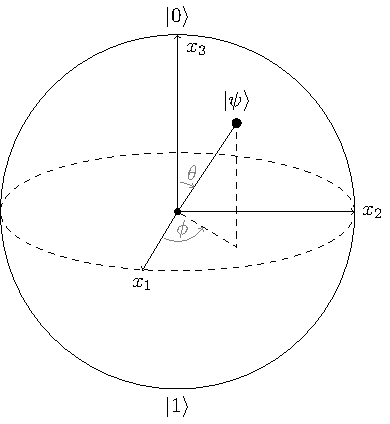
\includegraphics[width=0.7\textwidth]{images/quantum-information/bloch.pdf}
  \caption{Bloch-Kugel (Darstellung angelehnt an \cite{riebesell_scientific_2022})}\label{fig:bloch-sphere}
\end{figure}

Der Zustand des Qubits kann folgendermaßen berechnet werden:

\begin{equation}
  \ket{\psi} = \cos\frac{\theta}{2} \ket{0} + e^{i\phi} \sin\frac{\theta}{2} \ket{1}
\end{equation}

Ein Qubit kann also eine unendliche Anzahl an Zuständen annehmen. Das ließe die Vermutung zu, dass ein Qubit auch unendlich viele Informationen speichern kann. Dies ist jedoch nicht der Fall, weil beim Messen des Zustandes die Superposition zusammenfällt und das Qubit dann entweder den Wert $\ket{0}$ oder $\ket{1}$ hat. (vgl. [5 ff.]\cite{pattanayakQuantumMachineLearning2017}, \cite[15 f.]{nielsen_quantum_2010}

\subsection{Informationscodierung}
Thilo
\subsubsection{Basis Encoding}
Thilo

\subsubsection{QuAM Encoding}
\begin{itemize}
\item Ziel: Sammlung mehrerer Datenwerte und Speicherung im Quantenregister (Sammlung mehrerer Qubits, die gemeinsam einen Zustand beschreiben)
\item Quantenalgorithmus benötigt mehrere Zahlenwerte \( x_1, x_2, \ldots \) als Input
\item Daten in einem gemeinsamen Qubit-Register als Superposition von Basis-encodierten Zuständen speichern
\item Ergebnis: Gleichgewichtete Superposition aller Datenwerte mit Amplituden (hohe Wahrscheinlichkeiten gemessen zu werden)
\item Daten sind binär codiert (z.\,B. \( x_1 = 010, x_2 = 011, x_3 = 110 \))
\item Jeder Datenwert = ein Basiszustand im Quantenregister (z.\,B. \( |010\rangle \))
\item Für \( n \) Werte mit je \( l \) Bit: benötigt werden \( l \) Qubits
\end{itemize}
\cite{Date encoding patterns for quantum computing}
\\


Anwendungsbeispiel
\begin{itemize}
\item Gegeben: Drei Werte \( x_1 = 010 \), \( x_2 = 011 \), \( x_3 = 110 \)
\item Jeder Wert ist 3 Bit lang → 3 Qubits nötig
\item Quantenregister speichert:
  \[
  |\psi\rangle = \frac{1}{\sqrt{3}} (|010\rangle + |011\rangle + |110\rangle)
  \]
\item Nur diese drei Zustände haben Amplituden, alle anderen (z.\,B. \( |000\rangle, |001\rangle \)) = 0
\item Nach Messung: Einer der gespeicherten Werte wird mit Wahrscheinlichkeit \( \frac{1}{3} \) gelesen
\end{itemize}

\subsubsection{Angle Encoding}

\begin{itemize}
\item Jeder Datenpunkt wird durch ein separates Qubit repräsentiert.
\item Ziel: Daten effizient auf einem Quantencomputer kodieren, um möglichst viele Operationen innerhalb der Stabilitätsdauer des Quantenzustands durchzuführen.
\item Jeder Wert \(x_i\) wird auf das Intervall \([0, \frac{\pi}{2}]\) normalisiert.
\item Bereich \([0, \frac{\pi}{2}]\), weil \(\cos(x)\) und \(\sin(x)\) dort positiv sind → keine Vorzeichenprobleme
\item Ein einzelnes Qubit repräsentiert einen Datenwert durch  Rotation um die y-Achse auf der Bloch-Kugel.
\item Die resultierende Quantenzustand ist separabel, d.h. es findet keine Verschränkung der Qubits statt.
\item Der Zustand ergibt sich als Tensorprodukt einzelner Qubit-Zustände: 
\[
|\psi\rangle = \bigotimes_i \begin{bmatrix} \cos x_i \\ \sin x_i \end{bmatrix}
\]
\item Vorteil: Sehr effizient in Bezug auf Operationen – konstante Anzahl paralleler Einzelqubit-Rotationen genügt.
\item Nachteil: Für \(n\) Datenwerte werden \(n\) Qubits benötigt – nicht optimal im Qubit-Bedarf.
\item Anwendungen: Klassifikatoren, Quantum Image Processing (ein Qubit = Farbwert, Register = Position), Quantum Neural Networks (Quron).
\end{itemize}
\cite{encoding patterns for quantum algorithms}
\\


Anwendungsbeispiel:
\begin{itemize}
\item \textbf{Beispiel:} Temperaturen in Städten speichern – Berlin: 15°C, Paris: 25°C, Madrid: 30°C
\item \textbf{Schritt 1:} Normalisieren auf Bereich \([0, \frac{\pi}{2}]\)
  \begin{itemize}
    \item 15°C → 45°, 25°C → 75°, 30°C → 90°
  \end{itemize}
\item \textbf{Schritt 2:} Visualisierung: Jede Temperatur entspricht einem Zeiger (Qubit) auf einer Uhr
\item \textbf{Schritt 3:} Zeiger wird um Winkel gedreht (z.\,B. 45°)
\item \textbf{Schritt 4:} Drehung entspricht Rotation eines Qubits um y-Achse
\item \textbf{Schritt 5:} Jeder Qubit-Zustand speichert seinen Drehwinkel
\item \textbf{Schritt 6:} Kombination aller Qubits = Gesamtzustand des Systems
\end{itemize}


\subsubsection{QRAM Encoding}
Marvin
\subsubsection{Amplituden Encoding}
Marvin

\subsection{Verschränkung von Qubits}
\label{subsec:verschraenkungQubits}

Der eigentliche Nutzen von Qubits zeigt sich dann, wenn mehrere Qubits miteinander kombiniert werden. Während ein einzelnes Qubit sich in einer Überlagerung der Zustände \(0\) und \(1\) befinden kann, erweitert sich der gesamte Zustandsraum beim Hinzufügen weiterer Qubits \emph{exponentiell}.

In klassischen Computern führen \(n\) Bits zu \(2^n\) möglichen Kombinationen von festen Zuständen, wobei sich zu jedem Zeitpunkt aber immer nur \emph{eine} dieser Kombinationen im Arbeitsspeicher befindet. Ein klassisches 3-Bit-System kann zum Beispiel genau einen von acht Zuständen darstellen und gleichzeitig verarbeiten: \(000\), \(001\), ..., \(111\).

Ein Quantensystem aus \(n\) Qubits hingegen befindet sich in einer Superposition all dieser Zustände gleichzeitig. Es existieren also \(2^n\) sogenannte \emph{Basiszustände}, die gleichzeitig in der Beschreibung des Gesamtzustands mit bestimmten Gewichtungen (Wahrscheinlichkeitsamplituden) vorkommen. Der Gesamtzustand eines Qubit-Systems mit \(n\) Qubits kann somit als Superposition aller \(2^n\) möglichen klassischen Kombinationen dargestellt werden.

Jeder dieser Zustände kann gleichzeitig im Gesamtzustand des Systems enthalten sein – mit je einer komplexen Amplitude. Dies bedeutet nicht, dass der Quantencomputer alle Lösungen gleichzeitig kennt, aber dass er während der Berechnung in gewisser Weise mit vielen Möglichkeiten \emph{parallel} arbeiten kann. Dies ist ein einfacher Grund, warum manche Algorithmen auf Quantencomputern eine exponentielle Beschleunigung ermöglichen.

Je mehr Qubits man miteinander verschaltet, desto größer wird also der Zustandsraum. Schon mit wenigen Qubits lassen sich gewaltige Mengen an Zuständen darstellen und zum selben Zeitpunkt verarbeiten: Bei einem Qubit zwei Zustände, bei fünf 32, bei 50 \(\approx 1{,}13 \times 10^{15}\), \dots
An dieser Stelle soll zur Einordnung erwähnt werden, dass der Ende 2023 größte Quantencomputer 433 Qubits hat, das Unternehmen IBM aktuell jedoch einen Quantencomputer mit einer Anzahl von 100 000 Qubits plant.

Das verdeutlicht den fundamentalen Unterschied zwischen Quantencomputern und klassischen Computern in Bezug auf die Informationsverarbeitung. Ein Quantensystem mit $n$ Qubits operiert in einem $2^n$-dimensionalen komplexen Raum, wodurch es theoretisch alle $2^n$ Basiszustände gleichzeitig in einer Superposition verarbeiten kann. Wie eben aufgeführt wären dies für 50 Qubits \(\approx 1{,}13 \times 10^{15}\) (also über eine Billiarde) simultane Berechnungspfade. Bei einem klassischen Computer mit 50 Bits kann nur ein einziger Zustand zu jeder Zeit repräsentiert werden, weshalb diese Anzahl an Berechnungspfaden sequenziell abgearbeitet werden müsste.

Der mathematische Ausdruck für einen allgemeinen $n$-Qubit-Zustand lautet:
\begin{equation}
\ket{\psi} = \sum_{i=0}^{2^n-1} \alpha_i \ket{i}
\label{equ:n_qubit_zustand}
\end{equation}
wobei $\ket{i}$ die Basiszustände und $\alpha_i$ die komplexen Amplituden darstellen. Diese Superposition aller möglichen Basiszustände bildet die Grundlage für die exponentiell gesteigerte Verarbeitungskapazität von Quantencomputern gegenüber klassischen Systemen.

An dieser Stelle soll dargestellt werden, was das für ein 2-Qubit-System mit $n = 2$, also 4 Basiszuständen heißt. Die allgemeine Formel \ref{equ:n_qubit_zustand}
wird zu:
\begin{equation}
\ket{\psi} = \sum_{i=0}^{3} \alpha_i \ket{i} = \alpha_0 \ket{0} + \alpha_1 \ket{1} + \alpha_2 \ket{2} + \alpha_3 \ket{3}
\end{equation}

Die Basiszustände $\ket{0}$, $\ket{1}$, $\ket{2}$, $\ket{3}$ entsprechen den binären Darstellungen $\ket{00}$, $\ket{01}$, $\ket{10}$, $\ket{11}$. Daher lautet die explizite Darstellung:
\begin{equation}
\ket{\psi} = \alpha_0 \ket{00} + \alpha_1 \ket{01} + \alpha_2 \ket{10} + \alpha_3 \ket{11}
\end{equation}

Es ist wichtig zu beachten, dass diese theoretische Parallelität in der praktischen Anwendung durch die Eigenschaften der Quantenmessung und Dekohärenz begrenzt wird, dennoch stellt sie das fundamentale Prinzip dar, das Quantenalgorithmen ihre charakteristische Effizienz verleiht.

Diese enorme Zustandsvielfalt ist nicht einfach direkt auslesbar – bei einer Messung kollabiert das Qubit-System zu genau einem dieser \(2^n\) Basiszustände. Dennoch erlaubt die gleichzeitige Verarbeitung dieser vielen Möglichkeiten innerhalb eines Algorithmus ein grundsätzlich neues Rechenparadigma. Probleme, deren Rechenzeit auf konventionellen Computern exponentiell wächst können deshalb von Quantencomputern in angemessenen Zeiten gelöst werden. 

Es ist sehr wichtig Quantenparallelismus nicht mit dem parallelen Ausführen von Programmen in klassischen Computern gleichzusetzen. Quantenparallelismus nutzt die fundamentalen Eigenschaften der Quantenmechanik, insbesondere die Superposition und die Interferenz von Wahrscheinlichkeitsamplituden. Das heißt, dass es bei Quantenalgorithmen darum geht die Amplituden der Zustände so zu manipulieren, dass sich die Amplituden der Zustände, die korrekte Lösungen repräsentieren, durch konstruktive Interferenz verstärken, während sich die Amplituden der Zustände mit falschen Lösungen durch destruktive Interferenz abschwächen oder vollständig auslöschen. (vgl. \cite[16 f.]{nielsen_quantum_2010})

\section{Quanten-Gatter}\label{sec:quanten_gatter}
Quanten-Gatter sind die fundamentalen Operationen eines Quantencomputers. Sie manipulieren Qubit-Zustände auf kontrollierte Weise und bilden so das quantenmechanische Analogon zu klassischen Logikgattern. Im Gegensatz zu klassischen Gattern, bei dem ein Bit nur zwischen $0$ und $1$ wechselt, wirken Quanten-Gatter auf Superpositionen und können komplexere, zusammenhängende Zustände erzeugen.
\\
\subsection{Ein-Qubit-Gatter}
Ein klassisches \emph{Ein-Bit-Gatter} nimmt einen einzelnen Bitwert als Eingabe und liefert einen Bitwert als Ausgabe. Sein Verhalten lässt sich durch eine Wahrheitstabelle angeben – etwa invertiert das NOT-Gatter Eingaben $0 \rightarrow 1$ und $1 \rightarrow 0$. Abgesehen von der Identität ist NOT das einzige nicht-triviale Ein-Bit-Logikgatter in klassischen Computern. (Vgl. \cite[S.17f.]{nielsen_quantum_2010}) Dagegen transformiert ein \emph{Ein-Qubit-Gatter} den Zustand eines einzelnen Qubits. Strukturell handelt es sich um eine lineare, unitäre Abbildung im zweidimensionalen Zustandsraum. Konkret wird ein Ein-Qubit-Gatter durch eine, in Formel \ref{equq:unitaets} dargestellte, $2\times 2$-Unitärmatrix $U$ beschrieben, die den Zustandsvektor des Qubits auf einen neuen Zustand abbildet. (Vgl. ebd., S. 174)

\begin{equation}\label{equq:unitaets}
U = \begin{pmatrix}
a & b \\
c & d
\end{pmatrix}
\end{equation}
\\
Die Unitarität ($U^{\dagger}U = I$) stellt sicher, dass die Transformation physikalisch zulässig ist und rückgängig gemacht werden kann. Im Gegensatz zum klassischen Fall – mit nur einer nicht-trivialen Ein-Bit-Operation – existiert eine unendliche Vielfalt möglicher Ein-Qubit-Gatter, da jede $2\times 2$-unitäre Matrix ein gültiges Quantengatter repräsentiert. (Vgl. ebd.)\\

%In den folgenden Unterkapiteln \ref{subsec:pauli_gatter}, \ref{subsubsec:hadamard_gatter}, \ref{subsubsec:phase_shift_gatter} werden die in der folgenden Abbildung dargestellten Ein-Qubit-Gatter näher erläutert:


%https://www.tfp.kit.edu/downloads/lehre_2013_ss/aaa_HSS13_Grundlagen.pdf, Folie 13 --> Nur inspiriert, denke, dass kein Zitat notwendig ist


\newcommand{\gatterbox}[1]{%
  \tikz[baseline=-0.5ex]{
    \draw[-] (-1,0) -- (-0.3,0);
    \draw[thick] (-0.3,-0.4) rectangle (0.3,0.4);
    \node at (0,0) {\( #1 \)};
    \draw[-] (0.3,0) -- (1,0);
  }%
}
\[
\begin{array}{c@{\hspace{1cm}}c@{\hspace{1cm}}c}
\textbf{Pauli-X/Y/Z-Gatter} & \textbf{Hadamard-Gatter}\\
\gatterbox{X} & \gatterbox{H} 
\end{array}
\]

%& \textbf{Phase-Shift-Gatter} 
%& \gatterbox{R_\Theta}

\subsubsection{Pauli-Gatter $X$, $Y$, $Z$}\label{subsec:pauli_gatter}

Die Pauli-Matrizen wurden 1927 von dem Physiker Wolfgang Pauli eingeführt, um den neu entdeckten Elektronenspin im Rahmen der Quantenmechanik zu beschreiben. Elektronen besitzen einen intrinsischen Drehimpuls (Spin ½), der keine klassische Entsprechung hat. (Vgl. \cite[S.312]{wekesa_sirengo_mathematical_2024}) Pauli entwickelte drei $2\times 2$-Matrizen (oft $\sigma_x, \sigma_y, \sigma_z$ bezeichnet), um die Spin-$x$-, Spin-$y$- und Spin-$z$-Operatoren des Elektrons darzustellen. Dies geschah im Kontext der Erklärung des anomalen Zeeman-Effekts, bei dem Spektrallinien in Magnetfeldern aufgespalten werden. (Vgl. ebd.)\\
\\
In der üblichen Darstellungsform (der sogenannten $Z$-Basis ${|0\rangle,|1\rangle}$) lauten sie:
\\
\begin{equation}
\label{equ:pauli_matrizen}
  X=\begin{pmatrix}0&1\\ 1&0\end{pmatrix},\qquad
  Y=\begin{pmatrix}0&-i\\ i&0\end{pmatrix},\qquad
  Z=\begin{pmatrix}1&0\\ 0&-1\end{pmatrix}.
\end{equation}
\\
Jede Matrix ist dabei \emph{unitär}: Multipliziert man sie mit ihrer konjugiert-transponierten Version, erhält man wieder die Einheitsmatrix. (Vgl. \cite[S.71]{nielsen_quantum_2010}) Außerdem ist sie \emph{hermitesch}: Die Matrix ist ihr eigenes „Spiegelbild“. (Vgl. ebd., S.78) Beides zusammen bedeutet, dass wenn man ein Pauli-Gatter zweimal anwendet, steht das Qubit wieder da, wo es zuvor war ($U^2=I$). Es ergeben sich dabei ausschließlich die Eigenwerte $+1$ oder $-1$. Damit besitzt jeder Pauli-Operator genau zwei orthogonale Eigenzustände, was ihn zum einfachsten nicht-trivialen Messoperator macht. Weiterhin sind die Pauli-Matrizen spurlos, d.h. ihre Spur (die Summe der Diagonalelemente) ist null. (Vgl. ebd., S.76)\\
\\
Jeder Qubit-Zustand lässt sich, bezogen auf die in Unterkapitel \ref{subsec:blockkugel} eingeführte Block-Kugel, als Punkt auf einer Einheitskugel darstellen. In diesem Bild wirken die Pauli-Gatter wie Halbumdrehungen um die drei Raumachsen: $X$ rotiert den Bloch-Vektor um $180^{\circ}$ um die $x$-Achse, $Y$ um die $y$-Achse und $Z$ um die $z$-Achse. (Vgl. \cite[S.215ff.]{rieffel_quantum_2011}) Die Eigenzustände von $Z$ liegen daher an Nord- und Südpol, während die Eigenzustände von $X$ und $Y$ entlang des Äquators auf den $x$- bzw.\ $y$-Achsen sitzen.\\
\\
Die Wirkung der Ein-Quibit-Gatter Pauli-$X$-, $Y$-, $Z$-Gatter wird folgendermaßen beschrieben:



\begin{itemize}
\item Pauli-$X$ (Bit-Flip-Gatter): Vertauscht die Basiszustände $|0\rangle$ und $|1\rangle$. Es gilt: $X|0\rangle = |1\rangle$ und $X|1\rangle = |0\rangle$. (Vgl. ebd., S.81-82) Dieses Gatter entspricht somit einem quantenmechanischen NOT-Operator – analog zum klassischen Inverter (NOT-Gatter) flipping eines Bits. Aufgrund dieser Wirkung wird $X$ auch als Bitflip-Operator bezeichnet. 

\item Pauli-$Y$ (kombiniertes Gatter): $Y$ lässt sich als $Y = iZ \cdot X$ auffassen. Entsprechend kombiniert es eine Bit-Flip- und eine Phasenflip-Operation. Konkret gilt $Y|0\rangle = \mathrm{i},|1\rangle$ und $Y|1\rangle = -,\mathrm{i},|0\rangle$ (mit $\mathrm{i}=\sqrt{-1}$). Man sieht, dass $Y$ – ähnlich wie $X$ – $|0\rangle$ und $|1\rangle$ vertauscht, jedoch zusätzlich einen komplexen Phasenfaktor ($\pm,\mathrm{i}$) hinzufügt. (Vgl. ebd.) Im Ergebnis ist $Y$ somit ein Bit-Flip mit Phasendrehung und wird manchmal auch als kombiniertes Bit- und Phasenflip-Gatter bezeichnet.

\item Pauli-$Z$ (Phase-Flip-Gatter): Lässt $|0\rangle$ invariant und kehrt die Phase von $|1\rangle$ um. Das heißt, $Z|0\rangle = |0\rangle$, aber $Z|1\rangle = -,|1\rangle$. Für einen allgemeinen Qubit-Zustand $a|0\rangle + b|1\rangle$ bewirkt $Z$ also einen Phasenfaktor $-1$ für den $|1\rangle$-Anteil. (Vgl. ebd.) Durch das Verhalten des Vorzeichenwechsels, ergibt sich ebenfalls die Bezeichnung des Phasenflip-Gatters.

\end{itemize}\\
\\
Die Pauli-Gatter gehören meist zur Grundmenge der verfügbaren elementaren Quantenoperationen auf einem Qubit. Zusammen mit dem Einheitsoperator $I$ bilden sie die sogenannte Pauli-Gruppe auf einem Qubit. Komplexere Ein-Qubit-Gatter lassen sich durch Kombinationen der Pauli-Gatter darstellen. So ist etwa das weit verbreitete und im folgenden Unterkapitel \ref{subsubsec:hadamard_gatter} beschriebenen Hadamard-Gatter eine von den Pauli-Matrizen abgeleitete Transformation. Auch Kontrollgatter wie CNOT können unter Nutzung von Pauli-Operatoren konstruiert werden. (Vgl. \cite[S.312]{wekesa_sirengo_mathematical_2024})
\\
\subsubsection{Hadamard-Gatter}\label{subsubsec:hadamard_gatter}
Das Hadamard-Gatter $H$ ist eines der einfachsten Mittel, um aus einem allgemeinen Qubit-Zustand eine Überlagerung (Superposition) zu erzeugen.  Während ein Bit nur entweder 0 oder 1 sein kann, vermischt $H$ die beiden Basiszustände so, dass das Qubit  „halb 0, halb 1“ wird. (Vgl. \cite[S.19f.]{nielsen_quantum_2010})\\
\\
Formal schreibt man: (Vgl. \cite[S.76]{rieffel_quantum_2011})
\\
\begin{equation}
  H = \frac1{\sqrt2}\!
  \begin{pmatrix} 1 & 1 \\ 1 & -1 \end{pmatrix},
  \qquad
  H|0\rangle=\frac{|0\rangle+|1\rangle}{\sqrt2},
  \quad
  H|1\rangle=\frac{|0\rangle-|1\rangle}{\sqrt2}.
\end{equation}
\\
Die beiden resultierenden Zustände $|+\rangle$ und $|-\rangle$ liegen genau auf der Äquatorebene der Bloch-Kugel; $H$ entspricht dort einer $\pi$-Drehung um die Achse $\tfrac{x+z}{\sqrt2}$ (Vgl. ebd., S.22).\\
\\
Da $H$ involutorisch, also sein eigenes Inverse ($H^2=I$), ist, kehrt eine zweite Hadamard-Operation den Prozess exakt um.  Dies erklärt die Kurzformel $H$ \emph{"[...] beeing like a square-root of NOT [...]"}(\cite[S.19]{nielsen_quantum_2010}): einmal angewendet bewirkt es einen halben Bit-Flip (Superposition), zweimal angewendet ergibt sich der volle Flip zurück zum Ausgangszustand.\\
\\
Die Fähigkeit, Superpositionen mit nur einem Gate herzustellen, macht H unverzichtbar für viele Quantenalgorithmen.  Im Deutsch-Jozsa-Algorithmus (siehe Unterkapitel \ref{subsec_jasza}) oder in Grovers Suche präpariert $H^{\otimes n}$ aus $|00\ldots0\rangle$ eine gleichgewichtige Überlagerung aller $2^{n}$ Eingabewerte und ermöglicht so Quantenparallelismus (Vgl. ebd., S. 250ff.).  Ohne ein solches Gate gäbe es keine Interferenzeffekte und folglich keinen Geschwindigkeitsvorteil gegenüber klassischer Berechnung.

%\subsection{Phase-Shift-Gatter}\label{subsubsec:phase_shift_gatter}


\subsection{Mehr-Qubit-Gatter}
Mehr-Qubit-Gatter operieren auf mehreren Qubits gleichzeitig. Während Mehr-Bit-Gatter wie AND oder XOR nicht umkehrbar sind, können Quantengatter durch ihre unitärität umgekehrt werden. Ein Mehr-Qubit-Gatter wirkt dabei auf einem Tensorprodukt-Raum, also dem zusammengesetzten Zustandsraum mehrerer Qubits. Es erlaubt Operationen, die nicht separabel sind, d.h. sie lassen sich nicht auf die Wirkung einzelner Gatter auf jedes Qubit zurückführen.\\
\\
Zu der Klasse der Mehr-Qubit-Gatter zählt das \emph{SWAP}-Gatter, das zwei Qubit-Zustände vertauscht, das \emph{CNOT-Gatter}, welches ein Steuerbit verwendet um das zweite zu invertieren, das \emph{Toffoli-Gatter}, welches zusätzlich ein zwei Steuerbits verwendet, sowie das \emph{Fredkin-Gatter}, das zwei Zielbits konditional vertauscht. (Vgl. \cite[S.29, 156f.]{nielsen_quantum_2010})\\
\\
In den folgenden Unterkapiteln wird sowohl den CNOT- als auch den SWAP-Gatter ausführlich untersuchen.

\newcommand{\cnotbox}{%
  \tikz[baseline=-0.5ex]{
    \draw[-] (-1,0.5) -- (-0.3,0.5);
    \draw[-] (-1,-0.5) -- (-0.3,-0.5);
    \draw[thick] (-0.3,-0.9) rectangle (0.3,0.9);
    \node[rotate=90] at (0,0) {\(\scriptsize\text{CNOT}\)};
    \draw[-] (0.3,0.5) -- (1,0.5);
    \draw[-] (0.3,-0.5) -- (1,-0.5);
  }%
}

\newcommand{\swapgatter}{%
  \begin{tikzpicture}[baseline=(current bounding box.center)]
    \draw (-1,0.5) -- (1,0.5);
    \draw (-1,-0.5) -- (1,-0.5);
    \node at (0,0.5) {$\times$};
    \node at (0,-0.5) {$\times$};
    \draw (0,0.5) -- (0,-0.5);
  \end{tikzpicture}%
}

\[
\begin{array}{c@{\hspace{1cm}}c}
\textbf{CNOT-Gatter} & \textbf{SWAP-Gatter}\\
\cnotbox & \swapgatter
\end{array}
\]

\subsubsection{CNOT}\label{subsec:cnot_gatter}
Das Controlled-NOT Gatter (CNOT) besitzt ein Kontroll- und ein Zielqubit und bewirkt, dass der Zustand des Zielqubits genau dann mit einem Pauli-X (Bitflipping, dem klassischen NOT) invertiert wird, wenn das Kontrollqubit im Zustand $|1\rangle$ ist. (Vgl. \cite[S.20f., 177f.]{nielsen_quantum_2010}) Der CNOT-Gatter ist unitär und invertierbar und lässt sich in der $4\times 4$-Matrix wie folgt darstellen: (Vgl. ebd.) \\
\begin{equation}
\text{CNOT} = \begin{pmatrix}
1 & 0 & 0 & 0 \\
0 & 1 & 0 & 0 \\
0 & 0 & 0 & 1 \\
0 & 0 & 1 & 0
\end{pmatrix}
\end{equation} \\
In der Standardbasis der zwei Qubits ${|00\rangle, |01\rangle, |10\rangle, |11\rangle}$ transformiert ein CNOT-Gatter die Basiszustände folgendermaßen:
$|00\rangle ;\to; |00\rangle$
$|01\rangle ;\to; |01\rangle$
$|10\rangle ;\to; |11\rangle$
$|11\rangle ;\to; |10\rangle$
Das Kontrollqubit bleibt also unverändert, währenddessen das Zielqubit genau dann seinen Zustand wechselt, wenn dieses $|1\rangle$ war. (Vgl. \cite[S.21]{nielsen_quantum_2010})
\\
\begin{figure}[h]
\centering
\begin{tikzpicture}[line width=0.8pt,
    control/.style={fill=black, draw=black, shape=circle, minimum size=6pt, inner sep=0pt},
    target/.style={draw, shape=circle, minimum size=12pt, inner sep=0pt}
]
% --- Qubit-Leitungen ---
\draw (-0.6,1) -- (1.6,1);  % obere Leitung
\draw (-0.6,0) -- (1.6,0);  % untere Leitung
% --- CNOT: Kontrollpunkt ---
\node[control] (ctrl) at (0.5,1) {};
% --- CNOT: Zielkreis mit Pluszeichen ---
\node[target] (targ) at (0.5,0) {};
\draw (0.5,-0.2) -- (0.5,0.2);   % vertikale Linie im Plus
\draw (0.3,0) -- (0.7,0);        % horizontale Linie im Plus
% --- Verbindungslinie zwischen Control und Target ---
\draw (ctrl) -- (targ);
% --- Untertitel ---
%\node at (0.5,-0.8) {\small Darstellung eines CNOT-Gatters (Controlled-NOT-Gatter)};
\end{tikzpicture}
\caption{Darstellung des CNOT-Gatters (nach \cite[S.178]{nielsen_quantum_2010})}
\end{figure} \\
CNOT-Gatter spielt eine zentrale Rolle in der Quantenlogik, da es im Zusammenspiel mit Ein-Qubit-Gattern eine zweistufige Unitarität bildet und sich daraus jeder beliebige Quantum-Schaltkreis bilden lässt. (Vgl. ebd. S.191) Ein Beispiel, bei dem das CNOT-Gatter zur Verschränkung beiträgt, ist bei der Erzeugung von Bell-Zuständen - dieses Thema wird in Unterkapitel \ref{sec:bell_zustand} erläutert. Darüber hinaus bilden CNOT-Gatter die Grundlage für komplexere Operationen wie bspw. beim Toffoli-Gatter (CCNOT). (Vgl. \cite[S.5f.]{abughanem_toffoli_2025})



\subsubsection{SWAP}
Ein SWAP-Gatter vertauscht den Zustand zweier Qubits. Formal entspricht es der Abbildung $|a,b\rangle \mapsto |b,a\rangle$ mit $a,b \in \{0,1\}$. In der Standardbasis $\{|00\rangle, |01\rangle, |10\rangle, |11\rangle\}$ ergibt sich daraus folgende Matrix:

\begin{equation}
U_{\text{SWAP}} =
\begin{pmatrix}
1 & 0 & 0 & 0 \\
0 & 0 & 1 & 0 \\
0 & 1 & 0 & 0 \\
0 & 0 & 0 & 1
\end{pmatrix}
\end{equation}
\\
Diese Matrix vertauscht $|01\rangle$ und $|10\rangle$, während $|00\rangle$ und $|11\rangle$ unverändert bleiben. (Vgl. \cite[S.79]{rieffel_quantum_2011}) Der Gatter ist unitär, selbstinvers ($U^2 = I$) und hermitesch ($U = U^\dagger$). Damit erfüllt er alle Bedingungen für eine physikalisch zulässige Quantenoperation. (Vgl. \cite[S.2]{gheorghiuStandardFormQudit2011})\\
\\
Eine direkte Realisierung des SWAP-Gatters ist auf vielen Hardwareplattformen nicht vorgesehen. Stattdessen lässt es sich durch eine Folge von drei CNOT-Gattern konstruieren:
\begin{figure}[h]
\centering
\begin{tikzpicture}[line width=0.8pt, scale=1.2,
    control/.style={fill=black, draw=black, shape=circle, minimum size=4pt, inner sep=0pt},
    target/.style={draw, shape=circle, minimum size=10pt, inner sep=0pt},
    cross/.style={line width=0.8pt}
]

% --- Linien links ---
\draw (0,1) -- (3.5,1); % obere Leitung
\draw (0,0) -- (3.5,0); % untere Leitung

% --- CNOT 1 (oben kontrolliert) ---
\node[control] (c1) at (0.5,1) {};
\node[target]  (t1) at (0.5,0) {};
\draw (c1) -- (t1);
\draw (0.5,0) -- ++(-0.15,0);
\draw (0.5,0) -- ++(0.15,0);
\draw (0.5,-0.15) -- (0.5,0.15);

% --- CNOT 2 (unten kontrolliert) ---
\node[control] (c2) at (1.75,0) {};
\node[target]  (t2) at (1.75,1) {};
\draw (c2) -- (t2);
\draw (1.75,1) -- ++(-0.15,0);
\draw (1.75,1) -- ++(0.15,0);
\draw (1.75,0.85) -- (1.75,1.15);

% --- CNOT 3 (oben kontrolliert) ---
\node[control] (c3) at (3,1) {};
\node[target]  (t3) at (3,0) {};
\draw (c3) -- (t3);
\draw (3,0) -- ++(-0.15,0);
\draw (3,0) -- ++(0.15,0);
\draw (3,-0.15) -- (3,0.15);

% --- Gleichheitszeichen ---
\node at (4.1,0.5) {\LARGE $\equiv$};

% --- Linien rechts (SWAP) ---
\draw (5,1) -- (6.2,1);
\draw (5,0) -- (6.2,0);

% --- SWAP Gatter (gekreuzte X) ---
\draw[cross] (5.6,1.15) -- (5.8,0.85);
\draw[cross] (5.6,0.85) -- (5.8,1.15);
\draw[cross] (5.6,-0.15) -- (5.8,0.15);
\draw[cross] (5.6,0.15) -- (5.8,-0.15);
\draw (5.7,1) -- (5.7,0);

\end{tikzpicture}
\caption{Zerlegung des SWAP-Gatters in drei CNOT-Gatter (nach \cite[S.~23]{rieffel_quantum_2011})}
\end{figure}
\\
Ein zentrales Einsatzgebiet ergibt sich in Systemen mit begrenzter Konnektivität. Wenn zwei Qubits, die miteinander interagieren sollen, nicht direkt gekoppelt sind, werden SWAP-Gatter eingesetzt, um Zustände über benachbarte Qubits hinweg zu verschieben. Dieses Vorgehen ist unter dem Begriff \emph{Qubit-Routing} bekannt. (Vgl. \cite[S.2f.]{molaviQubitMappingRouting2022}) Auch in der Quanten-Fourier-Transformation wird das SWAP-Gatter verwendet. Am Ende der Transformation wird die spiegelverkehrte Reihenfolge der Qubits mithilfe von SWAP-Gattern wiederhergestellt, indem jeweils Paare symmetrisch zur Mitte des Registers vertauscht werden. (Vgl. \cite[S.219]{nielsen_quantum_2010})

%(Qubit Mapping and Routing via MaxSAT, S.2f.)


%\subsection{CU-Gatter}
%\subsection{Quantenschaltungen}


\section{Erste Algorithmen}
Algorithmen in der klassischen Informatik basieren alle auf einer linearen, schrittweisen Verarbeitung von Daten. So kann ein Bit, mit dem Wert 1 in einem folgenden Rechenschritt entweder den Wert 0 annehmen oder seinen aktuellen Wert 1 behalten. In einem Quantencomputer hingegen, kann das QBit nach einer Transformation unendlich viele verschiedene Werte annehmen.\\
\\
Mit dem Wissen aus vorherigen Kapitel lassen sich bereits die ersten, einfachen Quantenalgorithmen entwerfen, welche theoretisch schneller auf Quantencomputer ausgeführt werden können oder sogar für klassische Computer unmöglich sind zu lösen. \\
\\
Dazu beleuchten wir die Herkunft moderner Quantencomputer und die ersten Quantenalgorithmen.

\subsection{Algorithmus von Deutsch} 

In einem Paper von 1985 stellt der Physiker David Deutsch die Idee eines universellen Quantencomputers vor. Dabei verbindet er Quantenmechanik mit der theoretischen Informatik und kritisiert die klassische Church-Turing-These, da sie physikalisch nicht vollständig sei. Er schlägt stattdessen die Church–Turing–Deutsch-These vor: Alles, was physikalisch berechenbar ist, kann von einem Quantencomputer simuliert werden.\\
\\
Zentral im Paper ist der Vorschlag eines konkreten Quantenalgorithmus, welcher heute als der Deutsch-Algorithmus bekannt ist. Dieser zeigt, dass Quantencomputer Probleme effizienter lösen können als klassische Rechner.  (Vgl. \cite{deutsch_quantum_1985}) \\
\\
Wir wollen herausfinden ob ein Münze echt oder gefälscht ist. Bei einer echten Münze zeigen beide Seiten unterschiedliche Motive. Ist die Münze eine Fälschung, sind die Seiten gleich. Um eine echte Münze von einer Fälschung unterscheiden zu können, muss zuerst die Vorderseite und danach die Rückseite überprüft werden. In einem Quantencomputer können wir beide Seiten gleichzeitig prüfen. Das Überprüfen der Münze können wir als folgende binäre Funktion darstellen.

$$f:\{0,1\} \rightarrow \{0,1\}$$. 

Der Algorithmus von Deutsch möchte herausfinden, ob $f$ konstant (d.h. $f(0)=f(1)$) oder balanciert (d.h. $f(0)\neq f(1)$) ist. Übertragen wir das auf die Überprüfung der Münze, ist in dem Fall $f(0) = f(1)$ die Münze eine Fälschung und in dem Fall $f(0) \neq f(1)$ die Münze echt. \\
\\
Ein klassischer Computer muss beide Werte $f(0)$ und $f(1)$ abfragen. \\
\\
Deutsch zeigt, dass ein Quantencomputer mit nur einer Abfrage an ein Quanten-Orakel die Antwort liefern kann. Ein Quantenorakel ist dabei eine unbelichtete Funktion, welche $n$-Bits als Eingabe und $m$-Bits als Ausgabe liefert. Man könnte das Orakel auch als "Black Box" bezeichnen, deren Funktionsweise für unser Problem nicht relevant ist. Es ist also egal wie ein Computer die Münze überprüft, solange das Ergebnis der Prüfung einer Seite richtig ist. \\
\\
Um das Problem mit der Münze zu lösen, müssen wir eines der Quantenbits in eine Superposition über beide möglichen Eingaben von $f$ versetzten. Danach wird das Orakel angewendet und wir bekommen ein Superposition über beide Funktionswerte zurück.\\
\\
Damit das Problem für einem Quantencomputer lösbar ist, müssen alle Rechenschritte umkehrbar sein. Da $f$ in dem konstanten Fall nicht reversible ist muss ein zweites Quantenbit für den Algorithmus verwenden werde. Daraus ergibt sich folgender Funktionsaufruf. Die Operation $\oplus$ entspricht dabei einem exklusiven Oder.

$$
U_f: \left|x\right\rangle\left| y\right\rangle \rightarrow  \left|x, y \oplus f(x)\right\rangle
$$\\
\\
Jetzt kann auf das Problem der Algorithmus von Deutsch angewendet werden. Dieser löst das Problem in folgenden 4 Schritten:

\begin{enumerate}
    \item Initialzustand: Zwei QBits im Zustand
$$\left|x\right\rangle\left|y\right\rangle \leftarrow  \left|0\right\rangle \left|1\right\rangle$$
\item Anwenden des Hadamard-Gatters auf beide QBits erzeugt Superposition:
$$
\left|x\right\rangle\left|y\right\rangle \leftarrow  H\left|x\right\rangle H\left|y\right\rangle
$$
\item Anwendung des Orakels $U_f$:
 $$
\left|x\right\rangle\left|y\right\rangle \leftarrow  U_f\left|x\right\rangle\left|y\right\rangle
$$
    Durch die vorbereitete Superposition des Zielregisters wird die Funktion $f(x)$ in die Phase codiert.
\item Nach erneuter Hadamard-Transformation misst man:
 \begin{itemize}
     \item Hat $\left|x\right\rangle\left|y\right\rangle$ den Wert $\left|0\right\rangle\left|1\right\rangle$: Funktion ist konstant oder die Münze ist eine Fälschung
     \item Hat $\left|x\right\rangle\left|y\right\rangle$ den Wert $\left|1\right\rangle\left|1\right\rangle$: Funktion ist balanciert oder die Münze ist echt
 \end{itemize}
\end{enumerate}

\begin{table}[h]
    \centering
    \renewcommand{\arraystretch}{1.5}
    \begin{tabular}{p{3cm} p{8cm}}
        \textbf{Schritt} & \textbf{Beschreibung} \\ \hline
        1. Initialzustand &
        Zwei QBits im Zustand:
        
        \(\left|x\right\rangle\left|y\right\rangle \gets \left|0\right\rangle \left|1\right\rangle\)
        \\

        2. Erzeugen einer Superposition &
        Anwenden des Hadamard-Gatters auf beide QBits erzeugt Superposition:
        
        \(\left|x\right\rangle\left|y\right\rangle \gets H\left|x\right\rangle H\left|y\right\rangle\)
        \\

        3. Anwenden des Quantenorakels \(U_f\) &
        Durch die vorbereitete Superposition des Zielregisters wird die Funktion \(f(x)\) in die Phase codiert:
        
        \(\left|x\right\rangle\left|y\right\rangle \gets U_f\left|x\right\rangle\left|y\right\rangle\)
        \\

        4. Messen &
        Nach erneuter Hadamard-Transformation misst man:
        \begin{itemize}

         \item Hat $\left|x\right\rangle\left|y\right\rangle$ den Wert $\left|0\right\rangle\left|1\right\rangle$: Funktion ist konstant oder die Münze ist eine Fälschung
    
         \item Hat $\left|x\right\rangle\left|y\right\rangle$ den Wert $\left|1\right\rangle\left|1\right\rangle$: Funktion ist balanciert oder die Münze ist echt
    
     \end{itemize}
    \end{tabular}
    \caption{Schritte des Deutsch-Algorithmus}
    \label{tab:deutsch_algorithmus}
\end{table}

Daraus folgt der Schaltkreis in Abbildung \ref{fig:deutsch-schaltkreis}.
\begin{figure}
    \centering
    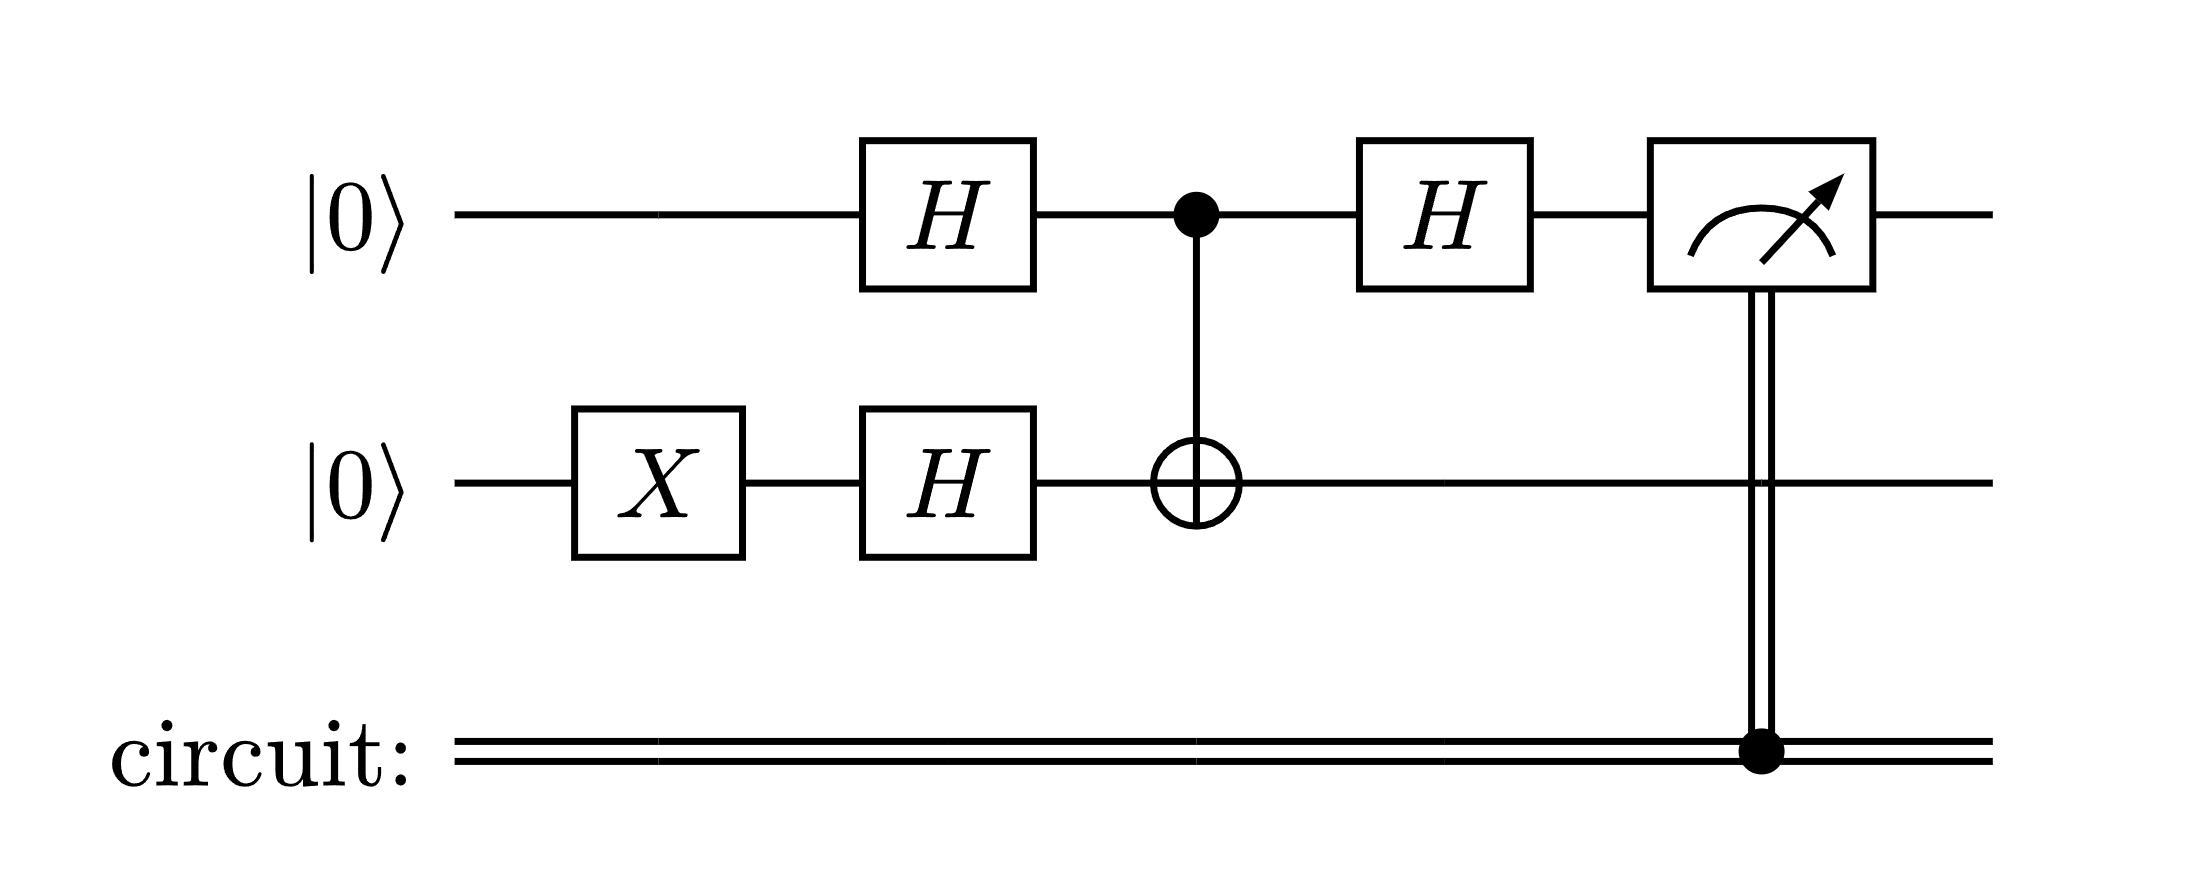
\includegraphics[width=1\linewidth]{images//quantum-information/deutsch schaltkreis.png}
    \caption{Schaltkreis: Deutsch-Algorithmus}
    \label{fig:deutsch-schaltkreis}
\end{figure}

Somit liefert Deutsch den ersten konkreten Algorithmus, welcher Quantenparallelität durch Superpositionen ausnutzt. Der von Deutsch vorgeschlagene Algorithmus ermöglicht es jedoch nur Probleme mit einem einzigen Eingabebit zu verarbeiten. Eine verallgemeinerte Version des Deutsch-Algorithmus lieferte David Deutsch zusammen mit Richard Jozsa ein paar Jahre später in dem Paper "Rapid solution of problems by quantum computation". (Vgl. \cite[S.33-37]{homeister_quantum_2022})

\subsection{Deutsch-Josza Algorithmus}\label{subsec_jasza}
Reale Probleme haben meist deutlich komplexere Strukturen und benötigen mehrere Eingabebits. Dazu entwickelten David Deutsch und Richard Jozsa eine Verallgemeinerung, welche als Deutsch-Jozsa-Algorithmus bekannt ist. Dieser erlaubt es, Funktionen mit beliebig vielen Eingabebits zu untersuchen und demonstriert erstmals einen exponentiellen Vorteil gegenüber klassischen Computern.\\
\\
Genau wie bei dem Deutsch-Algorithmus ist eine Funktion $f:\{0,1\}^n \rightarrow \{0,1\}$ gegeben. Dieses mal aber mit $n$-Bits als Eingabe. $f$ ist entweder konstant oder balanciert. Im balancierten Fall sind genau die Hälfte aller Ausgaben $0$ und die andere Hälfte $1$. (Vgl. \cite{deutsch_rapid_1992})\\
\\
Das Ziel bleibt unverändert. Es soll mit möglichst wenig Abfragen bestimmt werden, welcher der beiden Fälle vorliegt. Klassische Algorithmen benötigen für das Problem im schlimmsten Fall $2^{n-1}+1$ Abfragen, um Gewissheit zu erlangen. \\

Der Algorithmus läuft in folgenden Schritten ab:

\begin{enumerate}
\item Initialzustand:  Ein Register mit $n$ QBits im Zustand $\left|0\right\rangle^{\otimes n}$ und ein Hilfs-QBit im Zustand $\left|1\right\rangle$
\item Hadamard-Transformation auf alle QBits erzeugt eine Superposition:
$$
\left|x\right\rangle\left|y\right\rangle \leftarrow  H^{\otimes n}\left|0\right\rangle^{\otimes n} \otimes H\left|1\right\rangle
$$
\item Anwendung des Orakels $U_f$, das kohärent alle $2^n$ Eingaben verarbeitet:
$$
U_f \left|x\right\rangle\left|y\right\rangle = \left|x\right\rangle\left|y \oplus f(x)\right\rangle
$$
    Wie beim Deutsch-Algorithmus wird $f(x)$ in die Phase des Zustands eingeschrieben.
\item Erneute Hadamard-Transformation auf die ersten $n$ QBits.
\item Messung:
    \begin{itemize}
      \item Ergebnis $\left|0\right\rangle^{\oplus n}$ bedeutet die Funktion ist konstant
      \item Jedes andere Ergebnis bedeutet, die Funktion ist balanciert
    \end{itemize}
\end{enumerate}

\begin{table}[h]
    \centering
    \renewcommand{\arraystretch}{1.5}
    \begin{tabular}{p{3cm} p{8cm}}
        \textbf{Schritt} & \textbf{Beschreibung} \\ \hline

        1. Initialzustand &
        Ein Register mit \(n\) QBits im Zustand \(\left|0\right\rangle^{\otimes n}\) und ein Hilfs-QBit im Zustand \(\left|1\right\rangle\).
        \\

        2. Hadamard-Transformation &
        Anwenden von Hadamard-Gattern auf alle QBits erzeugt eine Superposition:
        
        \(\left|x\right\rangle\left|y\right\rangle \gets H^{\otimes n}\left|0\right\rangle^{\otimes n}\,\otimes\,H\left|1\right\rangle\).
        \\

        3. Anwendung des Orakels \(U_f\) &
        Das Orakel verarbeitet kohärent alle \(2^n\) möglichen Eingaben:
        
        \(
        U_f \left|x\right\rangle\left|y\right\rangle = \left|x\right\rangle\left|y \oplus f(x)\right\rangle.
        \)
        
        Wie beim Deutsch-Algorithmus wird \(f(x)\) in die Phase des Zustands eingeschrieben.
        \\

        4. Erneute Hadamard-Transformation &
        Auf die ersten \(n\) QBits wird erneut eine Hadamard-Transformation angewendet.
        \\

        5. Messung &
        Messung der ersten \(n\) QBits:
        \begin{itemize}
            \item Ergebnis \(\left|0\right\rangle^{\otimes n}\): Funktion ist konstant.
            \item Jedes andere Ergebnis: Funktion ist balanciert.
        \end{itemize}
        \\
    \end{tabular}
    \caption{Schritte des Deutsch-Jozsa-Algorithmus}
    \label{tab:deutsch_jozsa}
\end{table}


Abbildung \ref{fig:deutsch-jozsa-schaltung} zeigt einen entsprechenden Quantenschaltkreis mit 4 QBits. 
\begin{figure}
    \centering
    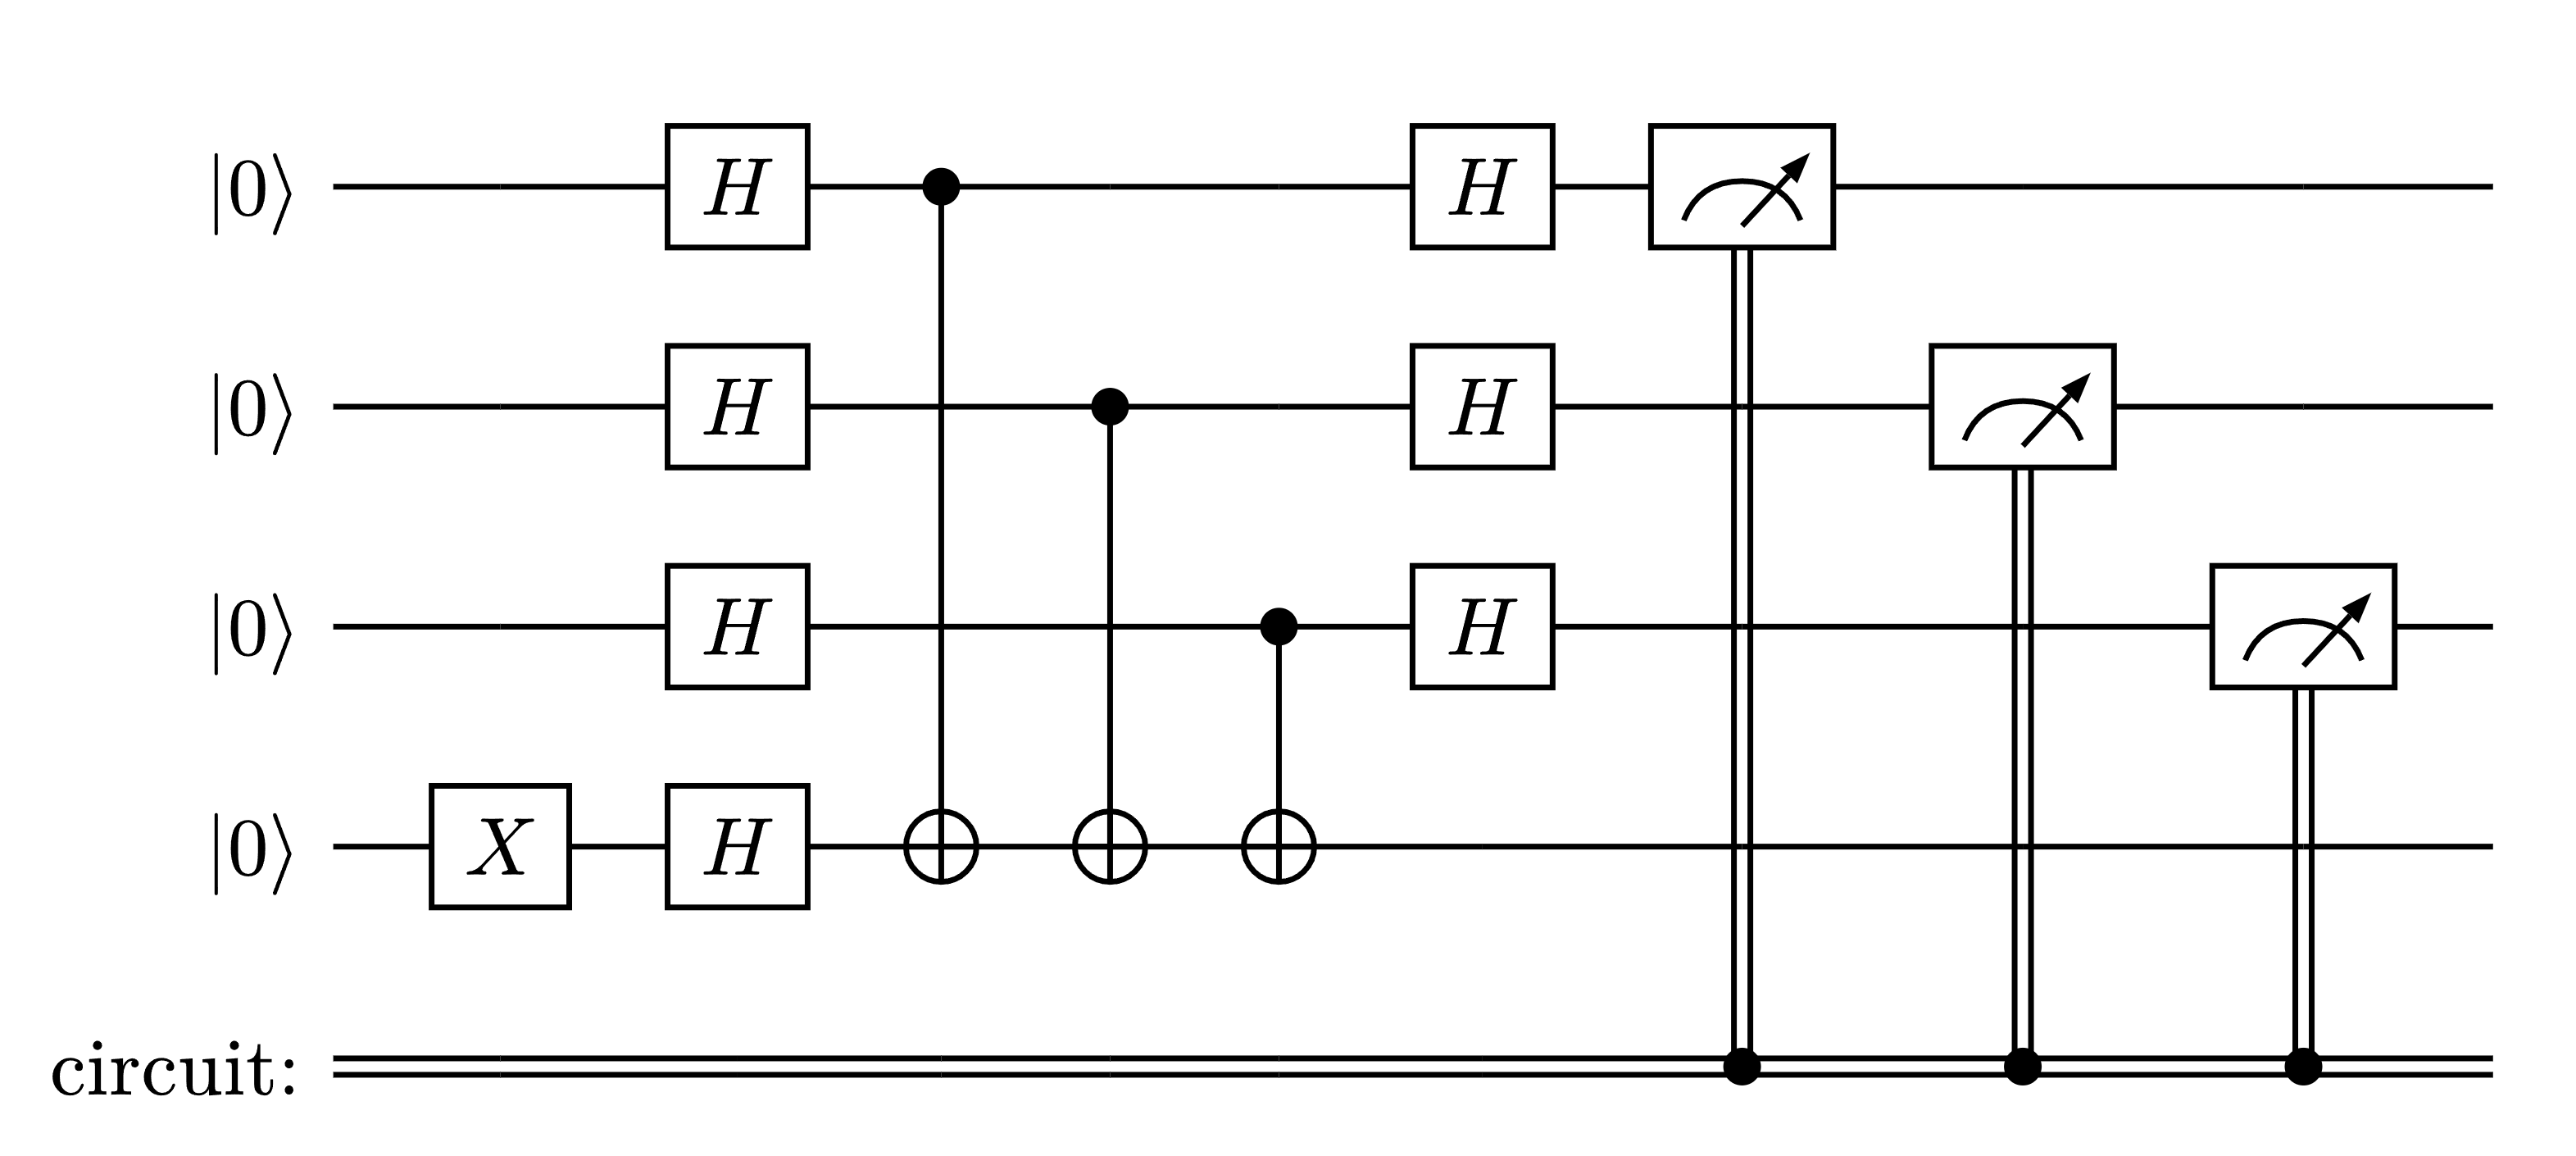
\includegraphics[width=1\linewidth]{images//quantum-information/deutsch-jozsa schaltkreis.png}
    \caption{Schaltkreis: Deutsch-Jozsa Algorithmus}
    \label{fig:deutsch-jozsa-schaltung}
\end{figure}

Das Besondere an dem Algorithmus ist, dass er das Ergebnis deterministisch und ohne Wahrscheinlichkeiten nach nur einer einzigen Orakelabfrage liefert. Durch Interferenz löschen sich bei balancierter Funktion die Amplituden für $\left|0\right\rangle^{\oplus n}$ vollständig aus. Nur im konstanten Fall bleibt sie erhalten. Somit liefert Deutsch und Jozsa den ersten theoretischen Beweis, dass Quantencomputer bei bestimmten Problemen klassischen Computern exponentiell überlegen sein können. (Vgl. \cite[S.62-66]{homeister_quantum_2022})





\section{Quantenverschränkung und Teleportation}

\subsection{Quantenverschränkung}
Quantenverschränkung ist ein Phänomen, bei dem zwei oder mehr Quantenobjekte sich in einem Zustand befinden, in dem sie, egal wie weit voneinander entfernt sie sind, gleich auf externe Reize reagieren. Solche Objekte, bei denen die Quantenverschränkung nachgewiesen werden konnte, sind Atome, Elementarteilchen wie Elektronen und Photonen, bis hin zu Kristallen.\\
\\
An einem Beispiel mit Elektronen lässt sich die Quantenverschränkung wie folgt erklären. Elektronen können sich in einem Zustand befinden, in dem sie keine eindeutige, exakte Position haben, sondern eine Menge an potentiellen Positionen. Diese potentiellen Positionen befinden sich alle im Umfeld der durchschnittlichen Position, dem Massenmittelpunkt des Elektrons, wie eine Wolke. Wenn von diesem Elektron seine Position gemessen wird, antwortet dieses Elektron auf die Messung mit einem zufälligen Wert. Bei den nächsten Messungen wird wiederum mit einem anderen zufälligen Wert geantwortet. Es besteht ein Indeterminismus. In diesem Zustand ist es sogar möglich, dass sich das Elektron, wegen dem Indeterminismus auch an zwei oder mehr Positionen gleichzeitig befindet. Und dieses Elektron, an zwei oder mehr Positionen gleichzeitig, reagiert auf Reize auf die gleiche Weise. Dies wurde im Doppelspaltexperiment von Thomas Young nachgewiesen, bei dem ein Elektron auf einen Reiz an der ersten Position an einem Young‘schen Spalt reagiert, und auf einen Reiz an der zweiten Position an einem anderen Young’schen Spalt reagiert.\\
\\
Obwohl es möglich ist, dass ein Quantenobjekt keine exakte Position hat, und ein weiteres mit dem ersten Quantenobjekt verbundenes, „verschränktes“ Quantenobjekt ebenfalls keine eindeutige Position hat, ist die Distanz zwischen den beiden Quantenobjekten klar bestimmt. Wenn man also die Position der beiden Quantenobjekte misst, erhält man für beide immer einen zufälligen Wert. Aber die Differenz der zufälligen Werte voneinander ist immer genau gleich. Das gilt immer, auch wenn die beiden Quantenobjekte sehr weit voneinander entfernt sind. Die Position eines Quantenobjekts selbst ist nicht wohlbestimmt, die Position im Bezug auf ein verbundenes, verschränktes Quantenobjekt hingegen schon. Dass sich ein Quantenobjekt „hier“ und „einer festen Distanz von hier“ gleichzeitig befindet, wird „Superposition“ genannt. Und dieser superpositionierte Zustand ist ein verschränkter Zustand.\\
\\
Die Verschränkung fixiert nicht nur die Distanz von zwei oder mehr Quantenobjekten voneinander, sondern auch weitere Variablen, z.B. die Geschwindigkeit. Sie haben die gleiche Geschwindigkeit, welche aber selbst nicht fest ist, sondern eine von einer Menge potentieller Geschwindigkeiten.\\
\\
(Vgl. \cite[S.83-88]{gisin_unbegreifliche_2014}) 

\subsection{Quantenteleportation - Übersicht}
Ein Objekt besteht aus Materie und physikalischem Zustand. Bei Quantenobjekten ist die Materie die Masse und permanente Attribute wie z.B. die elektrische Ladung bei Elektronen, bzw. die Energie bei massenlosen Quantenobjekten wie z.B. Photonen. Der physikalische Zustand besteht aus potentiellen, nicht eindeutigen Attributen, wie z.B. die potentiellen Positionen (Man denke die Positionen als Wolke um Massen-/ Energiemittelpunkt), die potentiellen Geschwindigkeiten bei Elektronen bzw. die potentiellen Schwingungsfrequenzen bei Photonen.\\
\\
In der Quantenteleportation wird der Zustand eines Quantenobjekts, der sog. Quantenzustand, ein Qubit, ohne das Durchlaufen einer Zwischenstrecke, also dem physischen Abstand der Quantenobjekte voneinander, von einer Position auf eine andere Position, vorausgesetzt, dass sich in dieser anderen Position ein Quantenobjekt derselben Art befindet, direkt versetzt. Die Masse bzw. Energie kann nicht teleportiert werden, weil dies das Prinzip der Unmöglichkeit von Kommunikation ohne Signalübertragung (Vgl. \cite[S.47-49]{gisin_unbegreifliche_2014})  verletzen würde. Dahingegen hat der Zustand weder eine Masse, noch eine Energie, denn sie ist potentiell – eine Wahrscheinlichkeit.\\
\\
Nach einer solchen Quantenteleportation verliert das Quantenobjekt seinen bisherigen Zustand und der neue Zustand entspricht dem Quantenzustand des zweiten Quantenobjekts vor der Quantenteleportation. Am Beispiel eines Photons kann man dies wie folgt erklären. Es gebe ein Photon mit gut strukturierter Polarisation. Bei solch einem Photon schwingt das elektrische Feld regelmäßig in eine bestimmte Richtung. Nach der Quantenteleportation verliert dieses Photon seine Struktur. Übrig bleibt ein depolarisiertes Photon, ein Photon mit strukturloser Polarisation, dessen elektrisches Feld unregelmäßig in alle Richtungen schwingt.\\
\\
Voraussetzung einer Quantenteleportation ist das Dasein einer Menge verschränkter Quantenobjekte. In der nächsten Subsektion wird hierüber genauer erläutert.\\
\\
(Vgl. \cite[S.124-128]{gisin_unbegreifliche_2014}) 


\subsection{Quantenteleportation - Hauptteil}
In einem theoretischen Szenario gibt ein Quantenobjekt eines Senders mit unbekanntem Quantenzustand bzw. Qubit \(\ket{\Phi}\). Dieser Qubit soll zu einem dritten Quantenobjekt eines Empfängers teleportiert werden. Der Sender ist im Besitz eines zweiten Quantenobjekts mit dem ursprünglichen Zustand \(\ket{\alpha_0}\), „Ancilla“ bzw. „Ancilla-Qubit“ genannt. Im ersten Schritt der Quantenteleportation bringt der Sender das Quantenobjekt mit dem Qubit \(\ket{\Phi}\) und das Quantenobjekt mit dem Ancilla-Qubit dazu, so miteinander zu interagieren, dass das erste Quantenobjekt in einen Standard Zustand \(\ket{\Phi_0}\), und das zweite Quantenobjekt in einen unbekannten Quantenzustand \(\ket{\alpha}\), welches die vollständige Information über \(\ket{\Phi}\) enthält, versetzt wird. Diese Interaktion ist eine gemeinsame Messung der Quantenzustände beider Quantenobjekte des Senders. Allerdings muss erwähnt werden, dass eine solche Messung nur ein positives Ergebnis liefert, wenn der Qubit \(\ket{\Phi}\) einem orthonormalen Set angehört. Dies bedeutet, dass die Qubit-Vektoren in diesem Set orthogonal zueinander sind, und gleichzeitig eine Norm von 1 haben. Im zweiten Schritt der Quantenteleportation wird dann die neue Ancilla, bzw. in anderen Worten das (positive) Ergebnis der Messung im ersten Schritt, an das Quantenobjekt des Empfängers gesendet, wonach der Empfänger die Qubit-Veränderung auslösende Interaktion vom Sender rückgängig machen kann, und somit eine Replikation des originalen Quantenobjekts mit dem Qubit \(\ket{\Phi}\) herstellen kann. Auf dieser Weise können Informationen von Quantenobjekten, also Quanteninformationen, ausgetauscht werden, ohne dass ein Quantenobjekt geklont wird, weil letzteres nach dem "No-Cloning-Theorem" (Vgl. \cite[S.77]{gisin_unbegreifliche_2014}) nicht möglich ist. Diese Methode der Quantenteleportation wird „spin-exchange“ genannt.\\
\\
(Vgl. \cite[S.1-2]{bennett_teleporting_1993})\\
\\
Am anfänglichen Zustand der „spin-exchange“ Methode sind das Quantenobjekt 2 auf der Senderseite und das Quantenobjekt 3 auf der Empfängerseite miteinander verschränkt. Durch die Interaktion auf Senderseite, wobei die Qubits der Quantenobjekte 1 und 2 verändert werden, wird die Verschränkung der Quantenobjekte 2 und 3 aufgehoben, und stattdessen die Quantenobjekte 1 und 2 verschränkt.\\
\\
(Vgl. \cite[S.2-3]{bennett_teleporting_1993})\\
\begin{figure}[h!]
    \centering
    \includegraphics[width=1.0\textwidth]{images/quantum-information/quantenverschränkung.png}
    \caption{Quantenobjekte als Würfel dargestellt}
    \label{fig:meinbild}
\end{figure}
\newpage
\noindent Mathematisch lässt sich der Prozess, wobei die Quantenobjekte in diesem Beispiel spin-\(\frac{1}{2}\) Partikel sind, mit folgenden Formeln darstellen:

\[ \ket{\Psi_{23}^{(-)}} = \sqrt{\frac{1}{2}} (\ket{\uparrow_2}\ket{\downarrow_3} + \ket{{\downarrow_2}\ket{\uparrow_3}}) \]
\\
Das zweite Quantenobjekt vom Sender (2) und das Quantenobjekt vom Empfänger (3) befinden sich in einem verschränkten Zustand. Dies ist die Ausgangssituation.

\[ \ket{\Psi_{12}^{(+)}} = \sqrt{\frac{1}{2}} (\ket{\uparrow_1}\ket{\downarrow_2} + \ket{{\downarrow_1}\ket{\uparrow_2}}) \]
\[ \ket{\Phi_{12}^{(\pm)}} = \sqrt{\frac{1}{2}} (\ket{\uparrow_1}\ket{\uparrow_2} \pm \ket{{\downarrow_1}\ket{\downarrow_2}}) \]
\\
Nun findet die gemeinsame Messung der beiden Quantenobjekte des Senders statt. Die vier sich in den Formeln befindenden Zustände bilden eine orthonormale Basis für die Quantenobjekte 1 und 2. Hiermit ist die Verschränkung der Quantenobjekte 2 und 3 aufgehoben, und stattdessen sind 1 und 2 verschränkt.

\[ \ket{\Phi} = \ket{\Phi_1} = a{\uparrow_1} + b{\downarrow_1} \]
\\
Für einfache Verständlichkeit wird der unbekannte Originalzustand von Quantenobjekt 1, \(\ket{\Phi}\), so geschrieben. Dabei ist \(|a|^2 + |b|^2 = 1\).\\
\\
(Vgl. \cite[S.2]{bennett_teleporting_1993})

\subsection{Quantenkommunikation per Quantenverschränkung}
In der Quantenkommunikation bzw. im Quanteninformationstransfer innerhalb eines Quantennetzwerks werden Qubits bzw. Quantenzustände über Quantenkanäle gesendet. Quantenkanäle verbinden entfernte Knoten in einem solchen Netzwerk. Diese Quantenkanäle haben eine sog. Absorptionslänge. Die Länge der Quantenkanäle, und damit die maximale Distanz zweier miteinander verbundenen Knoten in einem Quantennetzwerk, ist nur auf wenige Vielfache der Absorptionslänge begrenzt. Dies führt zum Problem, dass Quantenkanäle „eng“ und „laut“ (Originaltext „noisy“) sind, und die transportierten Qubits sich miteinander verschränken können, was zu einem Übertragungsfehler führen könnte.\\
\\
Eine Lösung, die Wahrscheinlichkeit solcher Übertrangungsfehler zu reduzieren, mit Hinnahme von einer größeren Menge an benötigten Ressourcen, ist es, einzelne Qubits in einen konkatenierten Quantencode (z.B. einen verschränkten Zustand einer Vielzahl von Qubits) zu kodieren, und Operationen an diesem Code durchzuführen, während es durch den Quantenkanal übertragen wird. Dies wird „Verschränkungsreinigung“ (vom Eng. „entanglement purification“) genannt und ermöglicht möglichst unverfälschten Quanteninformationstransfer und sichere Quantenkryptographie in „engen“ und „lauten“ Quantenkanälen.\\
\\
Und um unverfälschten Quanteninformationstransfer auch über längere Quantenkanäle sicherzustellen, kann ein Schema verwendet werden, wobei sog. „Quantenrepeater“ einen langen Quantenkanal in kürzere Segmente aufteilen, und die Verschränkungen separat bereinigen, bevor diese wieder aneinander gehängt werden. Im Übergang von einem Segment zum nächsten werden Quantenkorrelationen aufgebaut, basieren auf Korrelationen die innerhalb der einzelnen Segmente existieren.\\
\\
(Vgl. \cite[S.1-2]{dur_quantum_1999})

\subsection{Quantenteleportation in Quantencomputern}
Die Informationen in den folgenden Abschnitten befinden sich in der Quelle (Vgl. \cite[S.1-2]{gottesman_quantum_1999}).\\
\\
Die Wissenschaftler Daniel Gottesman und Isaac Chuang stellen eine Technik, eine Verallgemeinerung von Quantenteleportation vor, welche Quantenberechnung in Quantencomputern effizient und ressourcenarm zulässt. Dadurch werden bekannte fehlertolerante Protokolle für Quantenberechnung vereinigt. Mit dieser Technik der Quantenteleportation sollen Quanteninformationen in einen neuen Zustand transformiert werden. Dies ähnelt der Wirkung eines Quantengatters.\\
\\
Zwei Qubits werden durch ein CNOT (controlled NOT) Gatter (gate) teleportiert. Ein CNOT gate ist eine Komponente, die zwei verschränkte Qubits in einem Bell-Zustand (Zustand, in dem zwei Qubits maximal miteinander verschränkt sind; mehr dazu in Subsektion 1.5.1) aufnimmt und den zweiten Qubit, den sog. „target“ Qubit dreht, wenn der erste Qubit, das sog. „control“ Qubit, einen Wert von \(\ket{1}\) hat. Beim Durchgang werden Pauli-Matrix Operationen durchgeführt, welche die Quanteninformationen auf einen dritten Qubit übertragen.\\
\begin{figure}[h!]
    \centering
    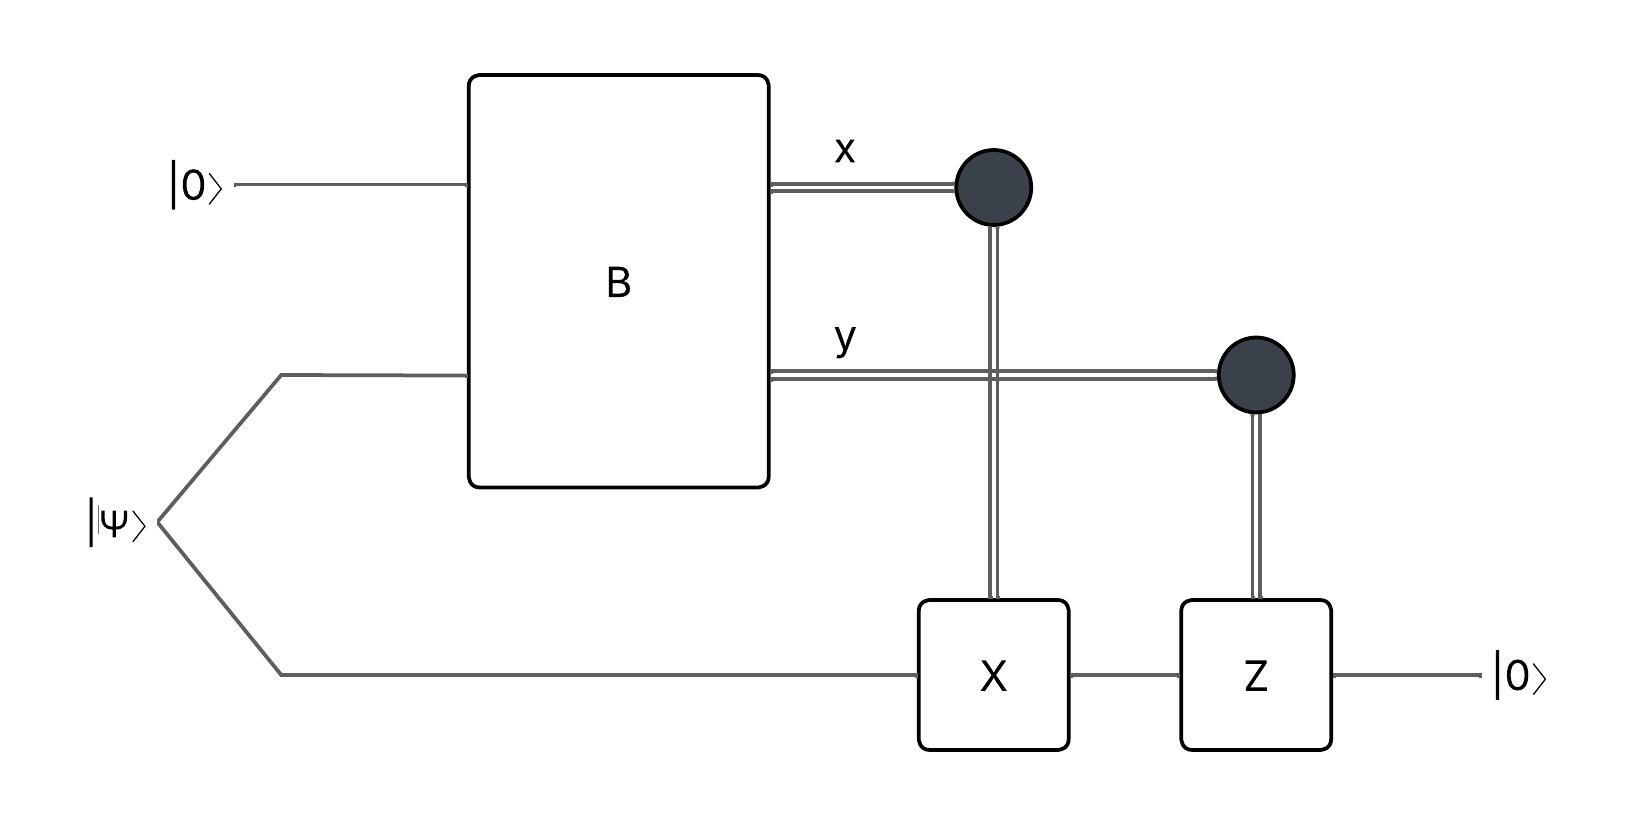
\includegraphics[width=1.0\textwidth]{images/quantum-information/quantenteleportation_cnot_1.jpeg}
    \caption{Zeitstrahl von links nach rechts. B = Bell-Zustand, X Y Z = Pauli Operatoren, \(\ket{0}\) = Zustand des Sender-Qubits, der an den Empfänger-Qubit übertragen werden soll}
    \label{fig:meinbild}
\end{figure}
\newpage
\noindent Dieses Prinzip kann leicht modifiziert werden. Die modifizierte Variante erlaubt es, vier Qubits, wovon jeweils zwei verschränkt sind, durchzulassen und anhand von Pauli-Matrix Operationen zu transformieren. Die zwei Paare von Verschränkungen sind vorerst getrennt. Eines enthält den „target“ Qubit \(\ket{\alpha}\), das andere den „control“ Qubit \(\ket{\beta}\). Der „target“ Qubit wird gedreht, wenn der „control“ Qubit einen Wert von \(\ket{1}\) hat. Es stehen 4 Rechenoperationen (I, X, Y, Z) zur Verfügung. Welche Operationen auf die Qubits der Verschränkungen angewendet werden, ist vom Zufall bestimmt. Zwei Qubits \(\ket{out}\), welche die Quanteninformationen von \(\ket{\alpha}\) und \(\ket{\beta}\) enthalten, wobei \(\ket{out}\) = CNOT\(\ket{\beta}\)\(\ket{\alpha}\), kommen aus den CNOT gate am Ende als Output heraus.\\
\begin{figure}[h!]
    \centering
    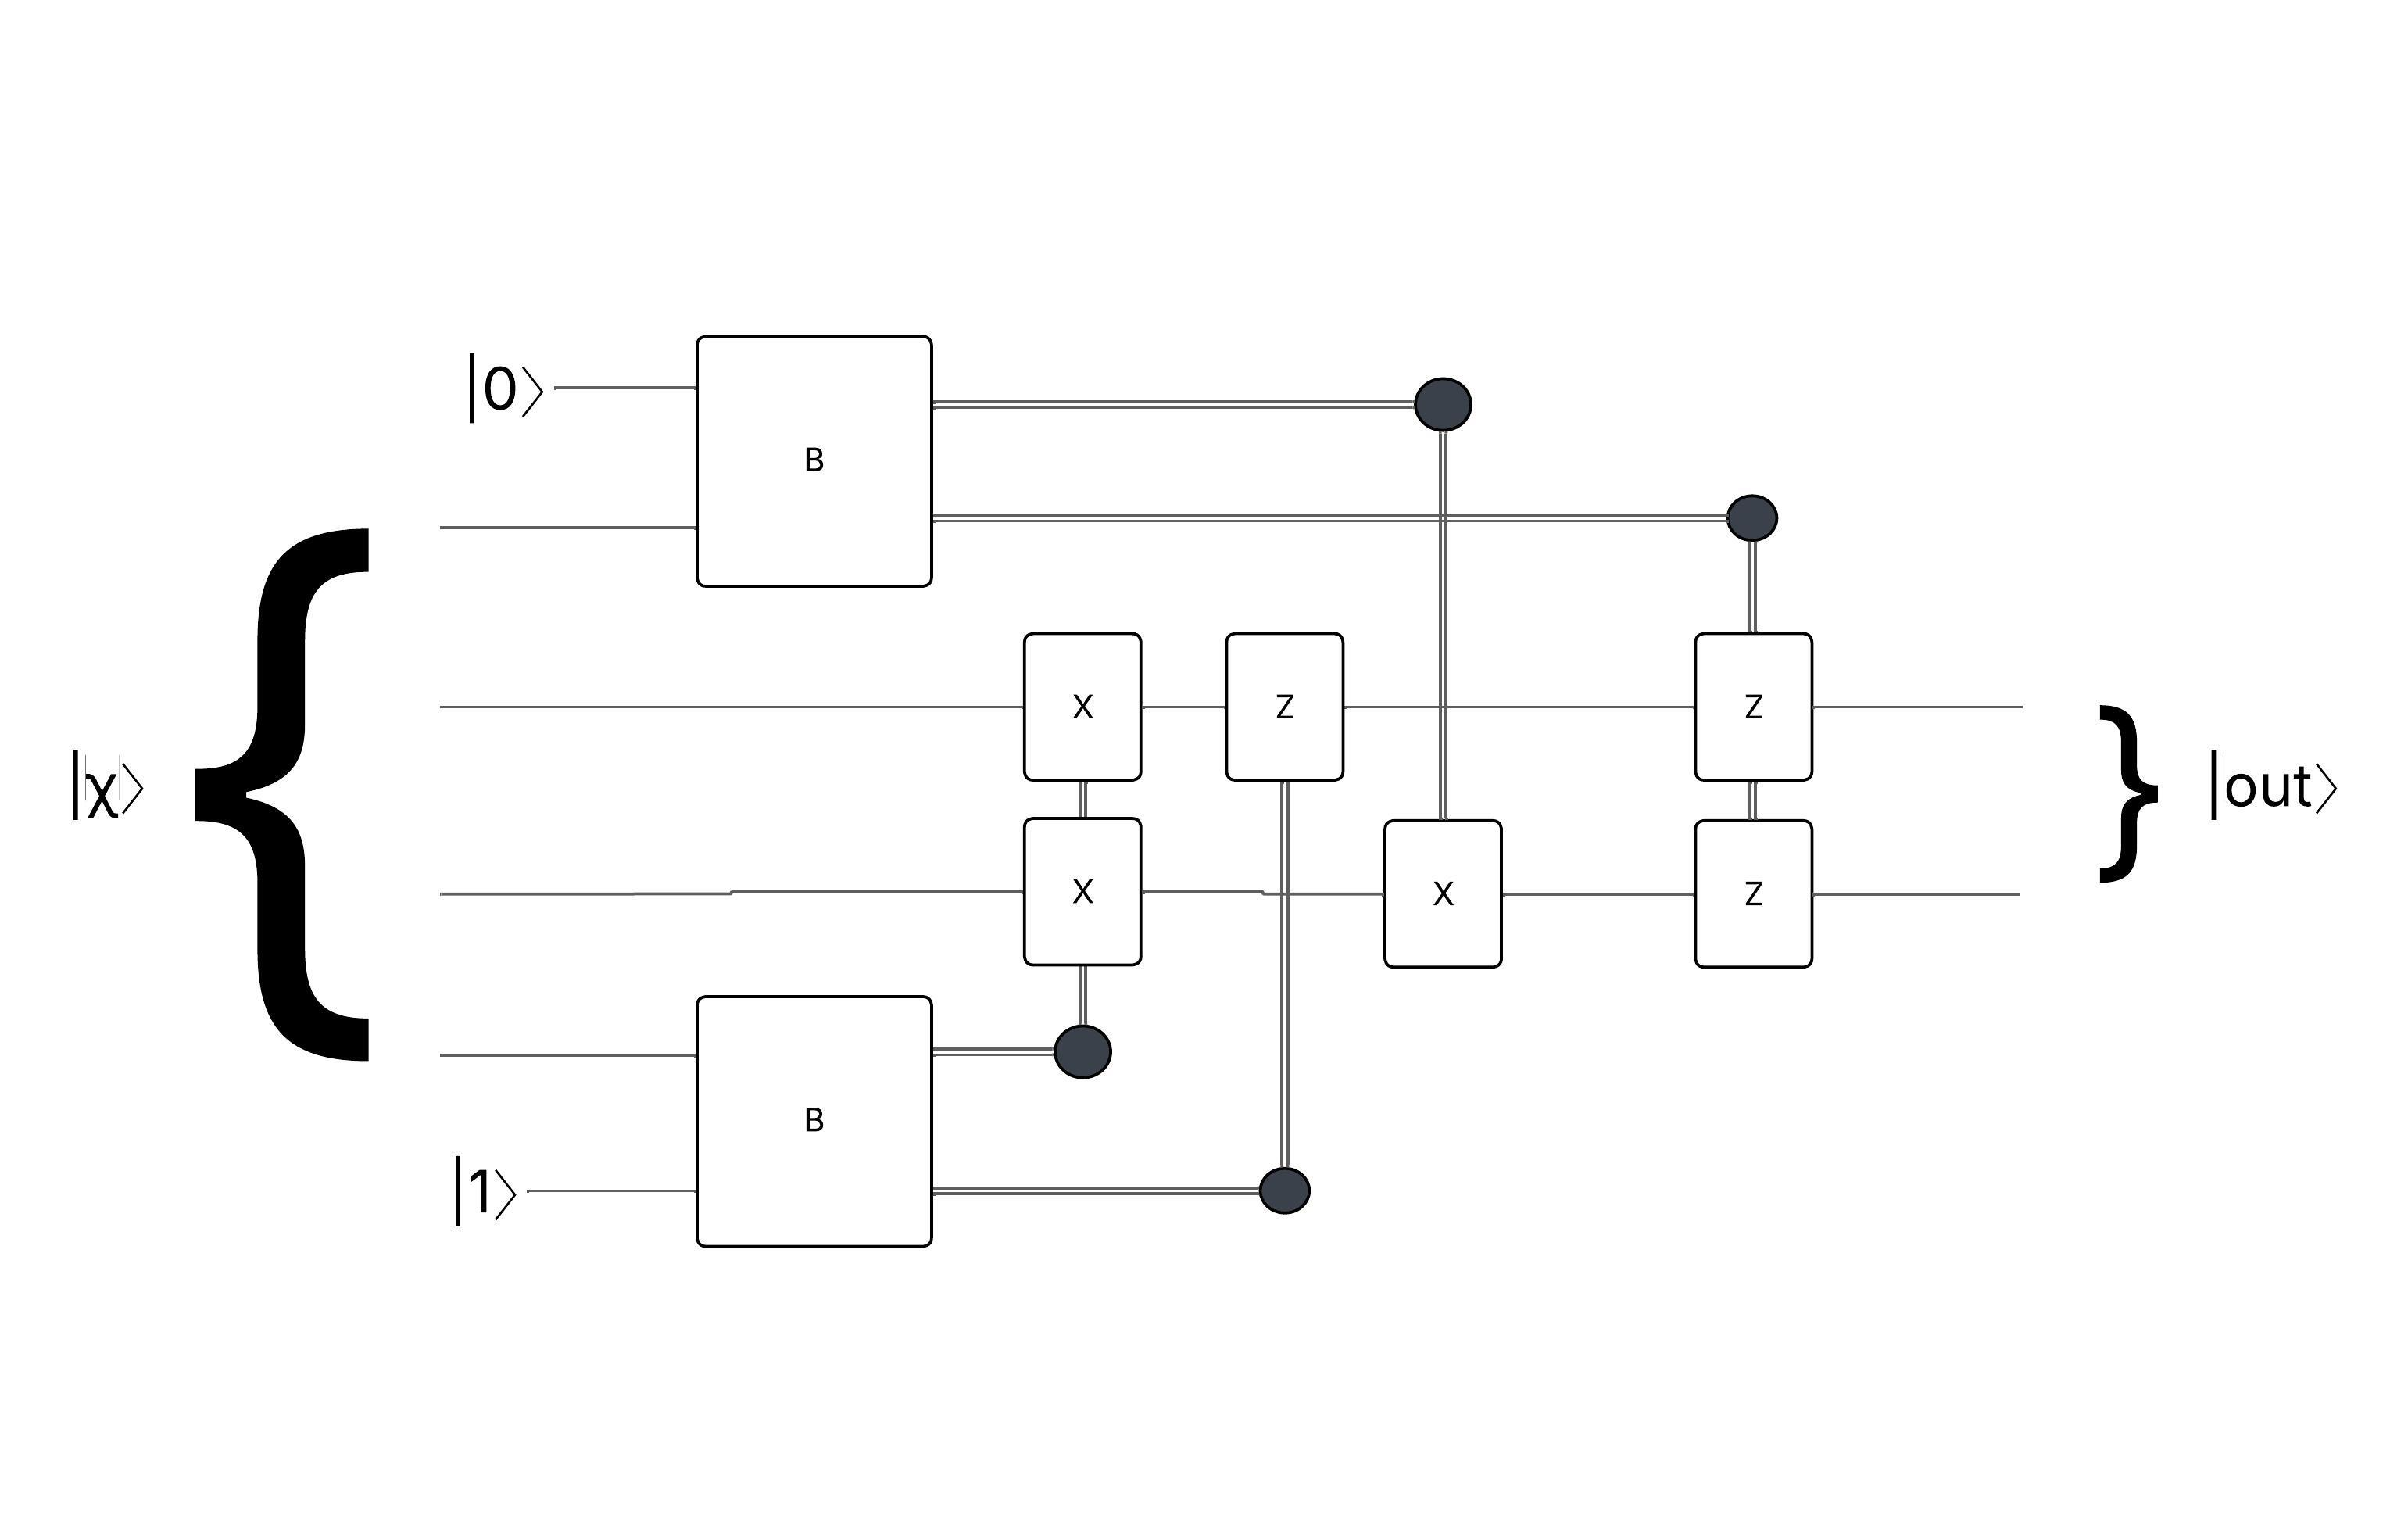
\includegraphics[width=1.0\textwidth]{images/quantum-information/quantenteleportation_cnot_2.jpeg}
    \caption{Zeitstrahl von links nach rechts. B = Bell-Zustand, X Y Z = Pauli Operatoren, \(\ket{\chi}\) = Ausgangszustand für Operation}
    \label{fig:meinbild}
\end{figure}
\newpage
\noindent Eine andere modifizierte Variante ist eine, bei der ein CNOT gate zwischen zwei Qubits von zwei unterschiedlichen verschränkten Qubit Paaren geöffnet wird. Der Output von solch einem Gatter kann verwendet werden, um den Zustand \(\ket{\chi}\) der vorherigen Abbildung zu bilden, von dem in einer Quantenteleportation mit zwei Verschränkungen Gebrauch gemacht wird. \(\ket{\chi}\) kann so erzeugt werden, oder durch eine Quantenteleportation zwischen zwei GHZ (Greenberger Horne Zellinger) Zuständen. Ein GHZ Zustand ist eine Verschränkung von drei Quantenobjekten.\\
\begin{figure}[h!]
    \centering
    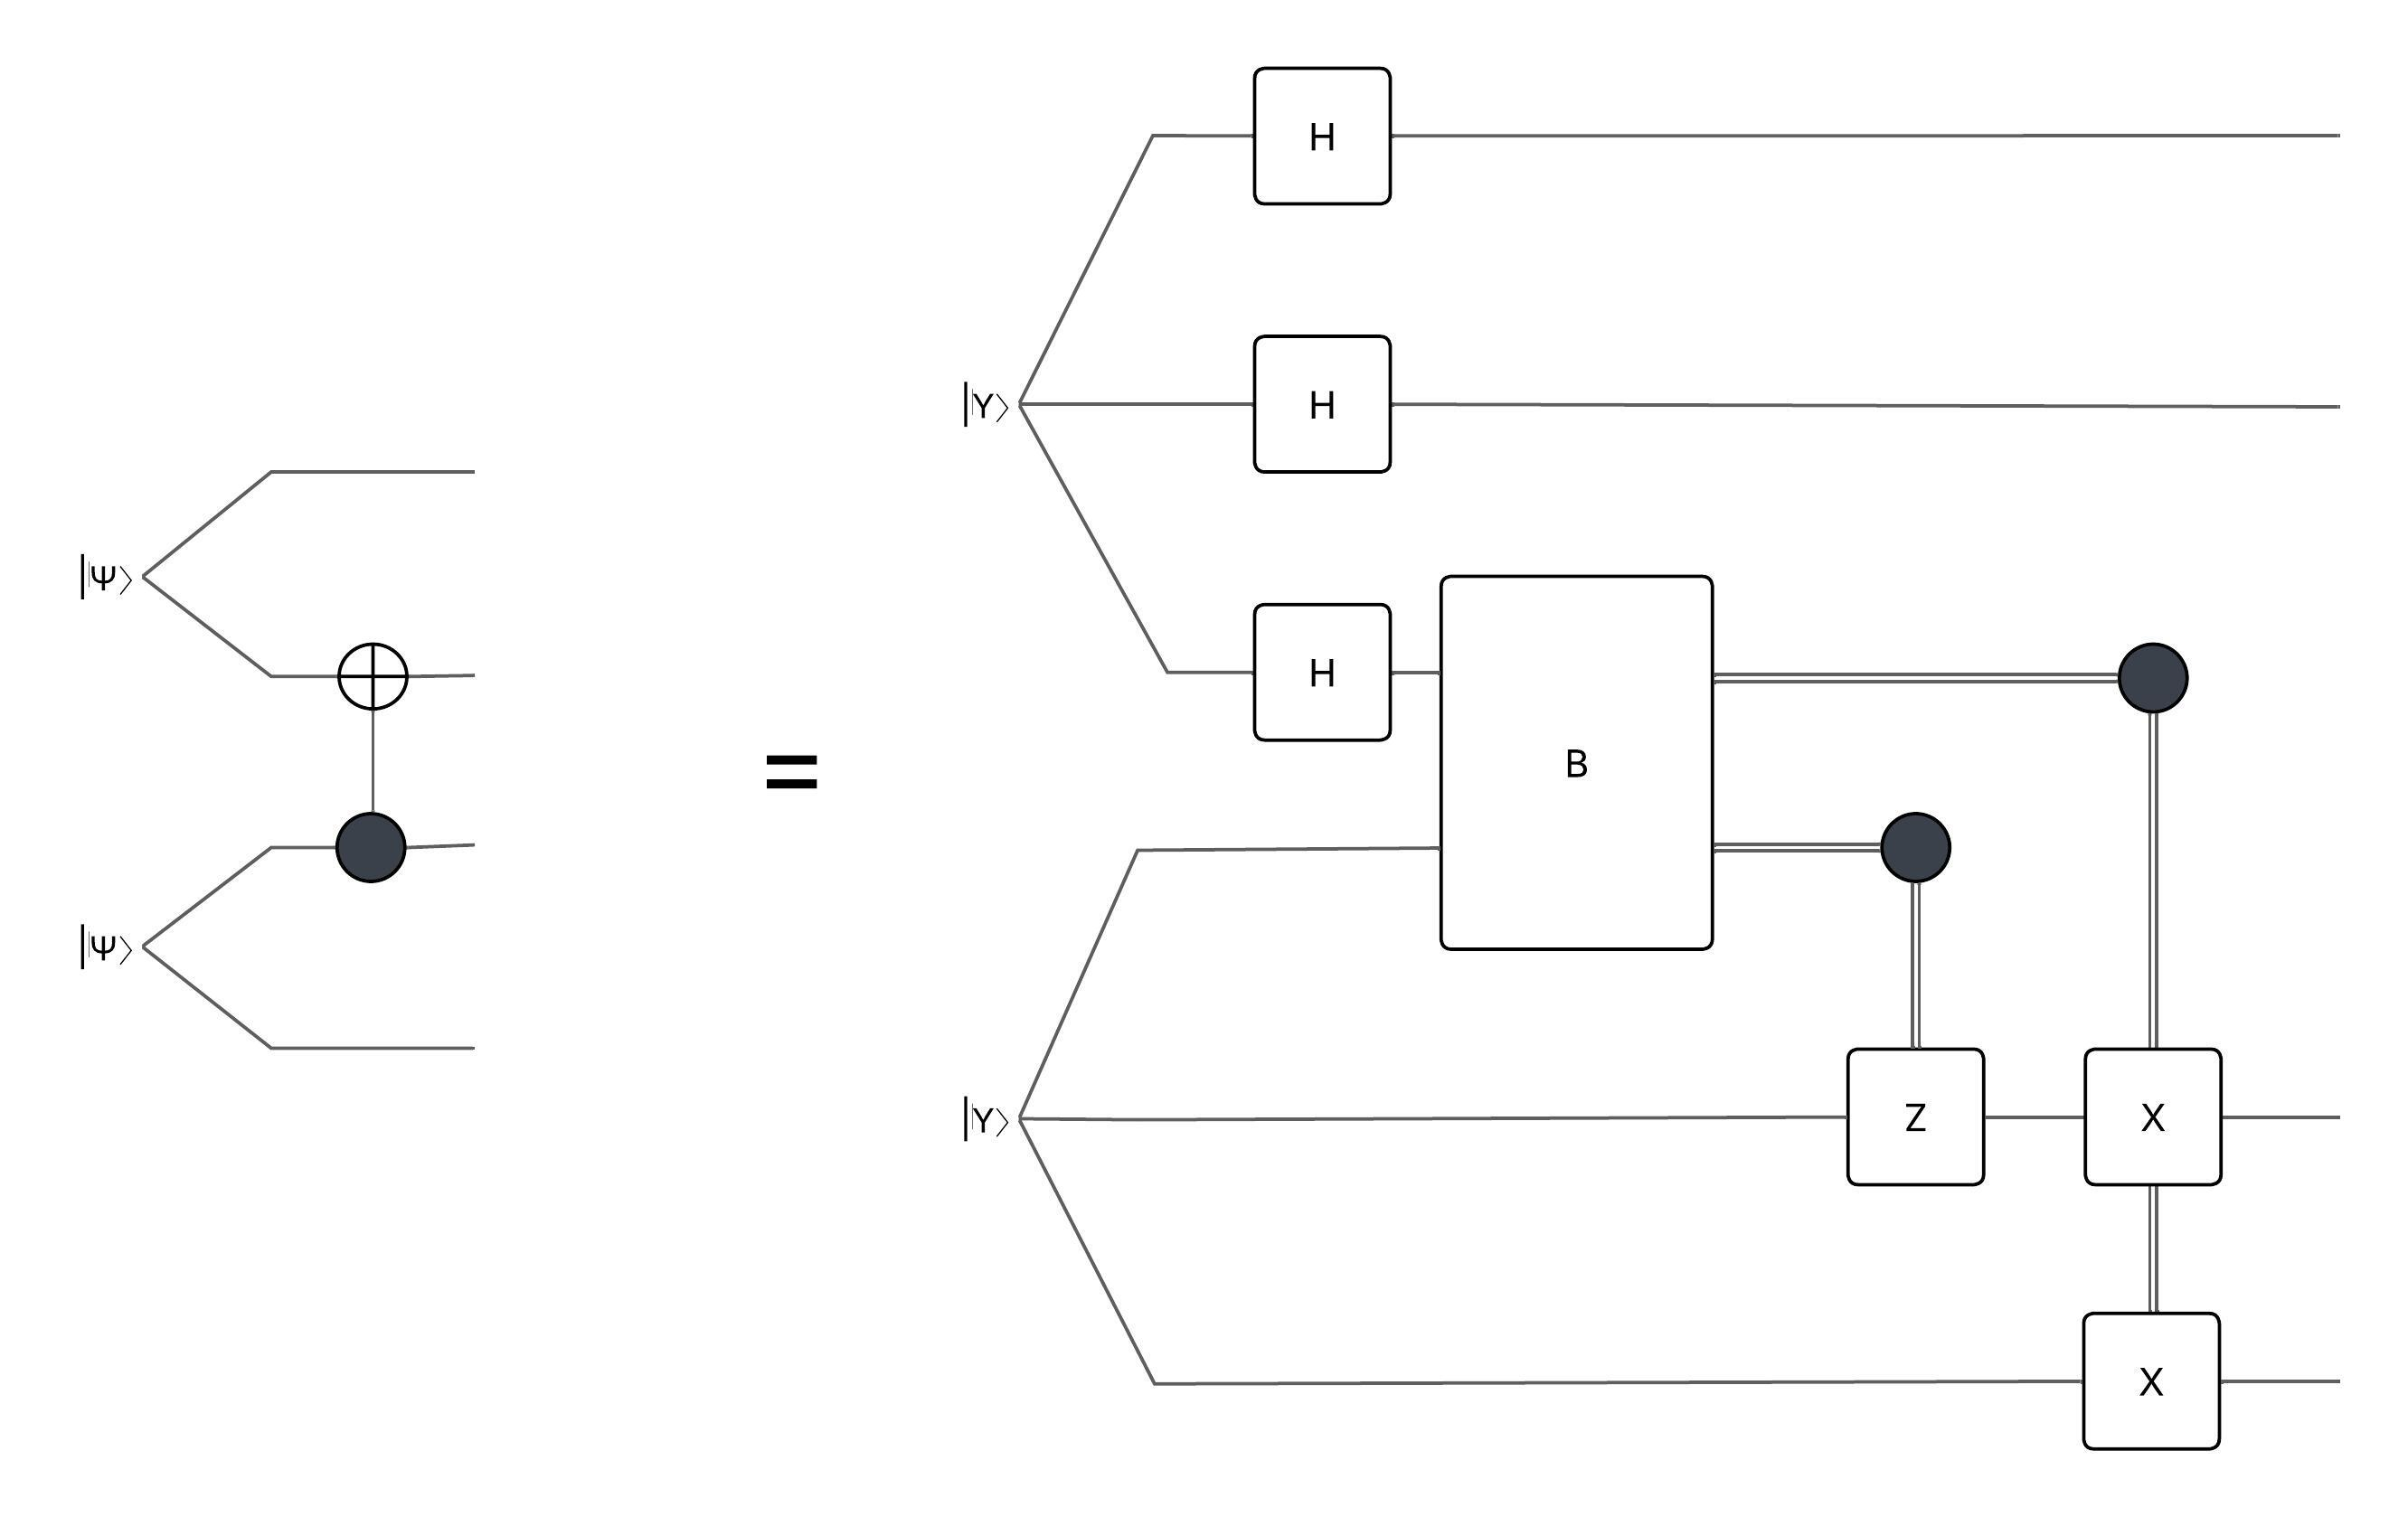
\includegraphics[width=1.0\textwidth]{images/quantum-information/quantenteleportation_cnot_3.jpeg}
    \caption{Zeitstrahl von links nach rechts. \(\ket{\Upsilon}\) = GHZ Zustand, H = Hadamard gate (für Hadamard Transformation), B = Bell-Zustand, X Z = Pauli Operatoren}
    \label{fig:meinbild}
\end{figure}
\newpage

\subsection{Bedeutung für Quantenkommunikation}
Wie Anhand der wissenschaftlichen Artikel von Bennett, Brassard et. al., sowie Gottesmann und Chuang gezeigt wurde, sind Quantenverschränkung und Quantenteleportation die Prinzipien, durch die es zu einem Quanteninformationstransfer kommen kann. Daraus kann man schließen, dass beide Prinzipien eine sehr wichtige Bedeutung für Quantenkommunikation haben.

\section{Fehlerkorrektur}
Qubits sind sehr fehleranfällig (mehr dazu ggf im Kapitel über physikalische Realisierung?). Im Gegensatz zu konventionellen Bits gestaltet sich die Fehlerkorrektur als schwieriger. Während konventionelle Bits kopiert und ausgelesen werden können, ist das bei Qubits nicht möglich, weil deren Superposition kollabieren würde, wenn man sie liest. Deshalb werden spezielle Quantenfehlerkorrekturverfahren entwickelt, die Fehler erkennen und beheben, ohne den Zustand der Qubits direkt zu messen. Diese Verfahren nutzen dabei die Verschränkung mehrerer Qubits, um Fehler zu detektieren und zu korrigieren, was allerdings einen erheblichen Mehraufwand an Qubits und Rechenressourcen erfordert.

In der Fehlerkorrektur sind insbesondere \emph{logische Qubits} wichtig. Ein logisches Qubit ist eine fehlerkorrigierte Version eines Qubits, die durch die Kodierung mehrerer physikalischer Qubits entsteht. Während ein physikalisches Qubit die tatsächliche quantenmechanische Implementierung darstellt, bildet ein logisches Qubit eine abstrakte Einheit, die durch redundante Kodierung vor Fehlern geschützt ist.

Die Funktionsweise basiert auf der Verteilung der Quanteninformation auf mehrere physikalische Qubits. Durch diese Redundanz können Fehler in einzelnen physikalischen Qubits erkannt und korrigiert werden, ohne die im logischen Qubit gespeicherte Information zu zerstören. 

Der Aufwand für die Implementierung logischer Qubits ist erheblich. Je nach verwendetem Fehlerkorrekturverfahren können hunderte oder sogar tausende physikalische Qubits erforderlich sein, um ein einzelnes logisches Qubit zu realisieren. Dieser Mehraufwand führt jedoch zu einer drastischen Verbesserung der Fehlerrate. Aktuelle Forschungsergebnisse zeigen, dass logische Qubits Fehlerarten aufweisen können, die um mehrere Größenordnungen niedriger sind als die ihrer physikalischen Komponenten. (vgl. \cite{divincenzoTopicsQuantumComputers1996}, \cite[426 ff.]{nielsen_quantum_2010}, \cite{ibm_research_team_introduction_nodate}).


\subsection{Beispiel: Bit-Flip}
Ein klassisches Beispiel für einen Fehler ist ein \emph{Bit-Flip}. Ein Bit-Flip liegt vor, wenn sich der Zustand eines Bits durch zum Beispiel kosmische Strahlung ungewollt ändert. Zur Fehlerkorrektur kann im Quantencomputing dann der sogenannte \emph{Bit-Flip-Code} verwendet werden. Dieser demonstriert hier das Grundprinzip logischer Qubits. Hierbei wird ein einzelnes logisches Qubit durch drei physikalische Qubits kodiert. Die Basiszustände werden dabei wie folgt abgebildet:

\begin{align}
\ket{0}_\text{logisch} &\rightarrow \ket{000}, \\
\ket{1}_\text{logisch} &\rightarrow \ket{111}.
\end{align}
Ein allgemeiner Qubit-Zustand
\begin{equation}
\ket{\psi} = \alpha \ket{0} + \beta \ket{1}
\end{equation}
wird somit als logischer Zustand kodiert zu:
\begin{equation}
\ket{\psi}_\text{logisch} = \alpha \ket{000} + \beta \ket{111}.
\end{equation}

Tritt ein Bit-Flip-Fehler auf einem der drei Qubits auf, entstehen fehlerhafte Zustände wie $\ket{001}$, $\ket{010}$ oder $\ket{100}$. Diese können durch eine \emph{Paritätsmessungen} erkannt und anschließend korrigiert werden, ohne die Amplituden $\alpha$ und $\beta$ zu zerstören.

Parität beschreibt in diesem Kontext, ob zwei Qubits denselben Zustand haben (also beide $\ket{0}$ oder beide $\ket{1}$) oder verschieden sind. Formal misst man die Parität zweier Qubits $i$ und $j$ durch den Operator:

\begin{equation}
 Z_i \cdot Z_j   
 \label{equ:parität_qubits}
\end{equation}


wobei $Z$ der Pauli-Z-Operator ist (vgl. Formel \ref{equ:pauli_matrizen}.

In der Praxis verwendet man ein Hilfsqubit (Ancilla), um diese Paritätsinformation indirekt zu messen. Der Ablauf ist wie folgt:

\begin{enumerate}
    \item Initialisiere das Ancilla-Qubit in Zustand $\ket{0}$.
    \item Wende zwei CNOT-Gatter an (vgl. Kapitel \ref{subsec:cnot_gatter}): 
    \begin{itemize}
        \item CNOT von Qubit $i$ auf das Ancilla-Qubit,
        \item CNOT von Qubit $j$ auf dasselbe Ancilla-Qubit.
    \end{itemize}
    \item Messe das Ancilla-Qubit in der Computational-Basis.
\end{enumerate}

Das Messergebnis liefert die Parität:
\begin{itemize}
    \item Ergebnis $\ket{0}$: Qubits $i$ und $j$ haben gleiche Parität ($\ket{00}$ oder $\ket{11}$),
    \item Ergebnis $\ket{1}$: Qubits haben unterschiedliche Parität ($\ket{01}$ oder $\ket{10}$).
\end{itemize}

Durch zwei Paritätsmessungen (z.B. zwischen Qubit 1–2 und 2–3) lässt sich ein einzelner Fehler eindeutig lokalisieren:

\begin{table}[h]
    \centering
\begin{tabular}{|c|c|c|}
\hline
Parität 1–2 & Parität 2–3 & Fehler in Qubit \\
\hline
gleich      & gleich      & keiner \\
ungleich    & gleich      & Qubit 1 \\
gleich      & ungleich    & Qubit 3 \\
ungleich    & ungleich    & Qubit 2 \\
\hline
\end{tabular}
   \label{tab:felherkorrektur}
\caption{Lokalisierung eines Fehlers in einem 3-Qubit-Sytems}
\end{table}


Das folgende Schaltbild zeigt die Paritätsmessung zwischen zwei Qubits mithilfe eines Ancilla-Qubits:

Sobald durch die Paritätsmessungen das fehlerhafte Qubit eindeutig identifiziert wurde (siehe Tabelle), wird der Fehler durch Anwendung eines Pauli-X-Gatters (Bit-Flip) auf das betroffene Qubit korrigiert. Das X-Gatter ist definiert als:

\[
X = \begin{pmatrix}
0 & 1 \\
1 & 0
\end{pmatrix},
\]

und wirkt auf die Basiszustände wie folgt:
\[
X\ket{0} = \ket{1}, \qquad X\ket{1} = \ket{0}.
\]

Beispielsweise:
\begin{itemize}
    \item Wenn Qubit 1 als fehlerhaft erkannt wurde (z.\,B. Zustand $\ket{100}$), wendet man $X$ auf Qubit 1 an:
    \[
    X_1\left( \alpha\ket{100} + \beta\ket{011} \right) = \alpha\ket{000} + \beta\ket{111}.
    \]
    \item Entsprechend für Qubit 2 oder 3.
\end{itemize}

Nach der Korrektur ist der logische Zustand wiederhergestellt:
\[
\ket{\psi}_\text{logisch} = \alpha\ket{000} + \beta\ket{111}.
\]

Die ursprüngliche Quanteninformation bleibt somit erhalten, obwohl ein physikalischer Fehler aufgetreten ist. Der Bit-Flip-Code demonstriert damit, wie Quantenfehler durch Redundanz und geeignete Messprotokolle erkannt und korrigiert werden können – ein grundlegendes Prinzip aller Quantenfehlerkorrekturverfahren. (vgl. \cite[426 ff.]{nielsen_quantum_2010})

\section{Bell-Zustand}\label{sec:bell_zustand}
Um die theoretischen Grundlagen der Quanteninformation greifbarer zu machen, bietet sich der Bell-Zustand als anschauliches Beispiel an. Er veranschaulicht zentrale Konzepte wie Quantenverschränkung und Nichtlokalität und bildet die Grundlage für viele Anwendungen in der Quantenkommunikation und -verarbeitung. Im Folgenden wird der Bell-Zustand näher erläutert, seine mathematische Darstellung vorgestellt und seine Bedeutung anhand konkreter Experimente und Anwendungen verdeutlicht.

\subsection{Was ist ein Bell-Zustand?}
Bell-Zustände sind spezielle Zustände in der Quantenmechanik, in denen zwei Teilchen maximal miteinander verschränkt sind. Das bedeutet: Ihre Zustände hängen so stark zusammen, dass man sie nicht unabhängig voneinander beschreiben kann – selbst, wenn die Teilchen physisch weit voneinander entfernt sind. Benannt ist der Bell-Zustand nach dem Physiker John S. Bell. Dieser zeigte im Jahre 1964 auf, dass die Vorhersagen der Quantenmechanik im Widerspruch zu den Prinzipien des lokalen Realismus stehen – also der Vorstellung, dass Informationen nicht schneller als Licht übertragen werden können und physikalische Größen vor der Messung bereits festgelegt sind. (Vgl. \cite[S.195]{bell_einstein_1964})
\\


Mit der von John S. Bell formulierten Bell-Ungleichung entwickelte Bell ein mathematisches Kriterium, mit dem sich klassische und quantenmechanische Theorien experimentell unterscheiden lassen. Die Quantenmechanik sagt unter bestimmten Bedingungen eine Verletzung der nach John S. Bell benannten Bell-Ungleichung voraus. Belegt wurde dies in zahlreichen Experimenten ab 1972, den sogenannten Bell-Test. Seitdem wurde die Verletzung der Bell-Ungleichung in zahlreichen Experimenten mit verschränkten Teilchenpaaren eindeutig nachgewiesen. In allen Fällen bestätigten die Ergebnisse die Vorhersagen der Quantenmechanik. 
(Vgl. \cite[S.53-59]{homeister_quantum_2022})

\subsection{Die vier Bell-Zustände}
Insgesamt existieren vier verschiedene Bell-Zustände, die eine Situation maximaler Verschränkung zwischen zwei Qubits beschreiben. Das heißt: Wird der Zustand eines Qubits gemessen, ist das Ergebnis des anderen automatisch bestimmt. Unabhängig von der Entfernung der Qubits voneinander. (Vgl. \cite[S.53-55]{homeister_quantum_2022}) 

\[
\begin{aligned}
\ket{\Phi^+} &= \frac{1}{\sqrt{2}} (\ket{00} + \ket{11}), \\
\ket{\Phi^-} &= \frac{1}{\sqrt{2}} (\ket{00} - \ket{11}), \\
\ket{\Psi^+} &= \frac{1}{\sqrt{2}} (\ket{01} + \ket{10}), \\
\ket{\Psi^-} &= \frac{1}{\sqrt{2}} (\ket{01} - \ket{10}).
\end{aligned}
\]

Mathematisch gibt es genau vier dieser Zustände, weil ein System aus zwei Qubits einen vierdimensionalen Zustandsraum besitzt. Die Bell-Zustände bilden darin eine vollständige Basis aller maximal verschränkten Zustände. Das heißt: Jede mögliche maximale Verschränkung zwischen zwei Qubits lässt sich als Kombination dieser vier Zustände ausdrücken.
\\


Die theoretischen Eigenschaften dieser Zustände lassen sich nicht nur mathematisch beschreiben, sondern auch ganz konkret auf Quantencomputern beobachten. In einer Simulation mit der IBM Quantum Learning Platform wurden hierfür zwei Qubits gezielt in einen verschränkten Zustand überführt. Das anschließende Messergebnis zeigt deutlich das charakteristische Verhalten eines Bell-Zustands: Es treten ausschließlich die Zustände \(\ket{00}\) und \(\ket{11}\) auf – jeweils mit 50\,\% Wahrscheinlichkeit. Die Kombinationen \(\ket{01}\) und \(\ket{10}\), bei denen sich die Qubits unterscheiden würden, wurden hingegen nicht beobachtet. Bemerkenswert ist dabei: Diese Quantenkorrelation bleibt bestehen, selbst wenn die Qubits räumlich voneinander getrennt sind. Die Messergebnisse des einen beeinflussen scheinbar sofort das andere – ein Verhalten, das mit klassischer Physik nicht erklärbar ist.

\begin{figure}[ht]
    \centering
    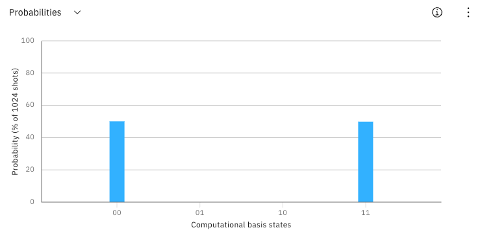
\includegraphics[width=1\textwidth]{images/quantum-information/results_ibm.png}
    \caption{Wahrscheinlichkeitsverteilung - IBM Quantum Learning Platform.}
    \label{fig:meinbild}
\end{figure}


\subsection{Erzeugung eines Bell-Zustands}
Für die Erzeugung eines Bell-Zustands werden zwei grundlegende Quantengatter benötigt: das Hadamard-Gatter und das CNOT-Gatter. Mithilfe dieser beiden Gatter kann eine Quantenschaltung realisiert werden, die jeden einfachen Zwei-Qubit-Eingangszustand (\(\ket{00}, \ket{01}, \ket{10}, \ket{11}\)) in einen Bell-Zustand überführt.

\begin{figure}[h]
  \centering
  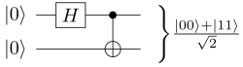
\includegraphics[width=0.4\textwidth]{images/quantum-information/bell_circuit.png}
  \caption{Quantenschaltung zur Erzeugung des Bell-Zustands}
\end{figure}

Die Erzeugung eines Bell-Zustands basiert auf zwei Schritten. Zu Beginn wird eine Superposition erzeugt, anschließend muss die Verschränkung zwischen den Qubits hergestellt werden. Diese Schritte werden nachfolgend erläutert.
\\


\textbf{Schritt 1 – Superposition erzeugen:} \\
Zuerst wird auf das erste Qubit ein Hadamard-Gatter angewendet. Dadurch wird dieses Qubit in eine Superposition überführt:

\[
\frac{1}{\sqrt{2}} (\ket{0} + \ket{1}) \ket{0} = \frac{1}{\sqrt{2}} (\ket{00} + \ket{10})
\]
\\


\textbf{Schritt 2 – Verschränkung herstellen:} \\
Anschließend folgt ein CNOT-Gatter, bei dem das erste Qubit als Kontroll- und das zweite als Zielqubit fungiert. Dieses Gatter invertiert das Zielqubit nur dann, wenn das Kontrollqubit den Zustand \(\ket{1}\) hat. Dadurch entsteht der Zustand:

\[
\frac{1}{\sqrt{2}} (\ket{00} + \ket{11}) = \ket{\Phi^+}
\]


Es resultiert einer der zuvor vorgestellten Bell-Zustände – ein maximal verschränkter Zustand, in dem die Messungen der beiden Qubits perfekt korreliert sind. Wird in einem verschränkten Bell-Zustand das erste Qubit gemessen, so ergibt sich mit gleicher Wahrscheinlichkeit entweder der Zustand \( \ket{0} \) oder \( \ket{1} \). In beiden Fällen legt diese erste Messung sofort auch den Zustand des zweiten Qubits fest: Beobachtet man \( \ket{0} \) am ersten Qubit, ergibt sich insgesamt der Zustand \( \ket{00} \); misst man \( \ket{1} \), resultiert der Zustand \( \ket{11} \). Eine anschließende Messung des zweiten Qubits führt daher zwangsläufig zum gleichen Ergebnis wie beim ersten – entweder beide Qubits liefern 0 oder beide liefern 1. Je nach Eingangs-Zustand und der Reihenfolge der Gatter ergibt sich ein anderer Bell-Zustand. (Vgl. \cite[S.53-54]{homeister_quantum_2022})
\\


Ein anschauliches Beispiel für die Eigenschaften verschränkter Zustände liefert ein Gedankenexperiment mit Alice und Bob. Angenommen die beiden erzeugten gemeinsam entsprechend der vorhergehenden Ausführungen folgenden Bell-Zustand:

\[
\begin{aligned}
\ket{\Phi^+} &= \frac{1}{\sqrt{2}} (\ket{00} + \ket{11}),
\end{aligned}
\]

Alice erhält nun das erste Qubit, Bob das zweite Qubit. Angenommen die beiden bewegen sich, wie nachfolgend abgebildet, anschließend in einem Haus in verschiedene Räume. Solange nun keine Messung erfolgt und die Qubits vor äußeren Einflüssen geschützt sind, bleibt die Verschränkung erhalten. Führen Alice oder Bob eine Messung durch, so ist das Ergebnis: Mit einer Wahrscheinlichkeit von 50\,\% wird $|0\rangle$ gemessen, mit 50\,\% $|1\rangle$. Erst wenn Alice und Bob ihre Ergebnisse miteinander vergleichen, zeigt sich die Besonderheit: Ihre Messergebnisse stimmen stets überein. Es resultiert eine perfekte Korrelation, unabhängig von Raum und Zeit. (Vgl. \cite[S.54]{homeister_quantum_2022})


\begin{figure}[h]
  \centering
  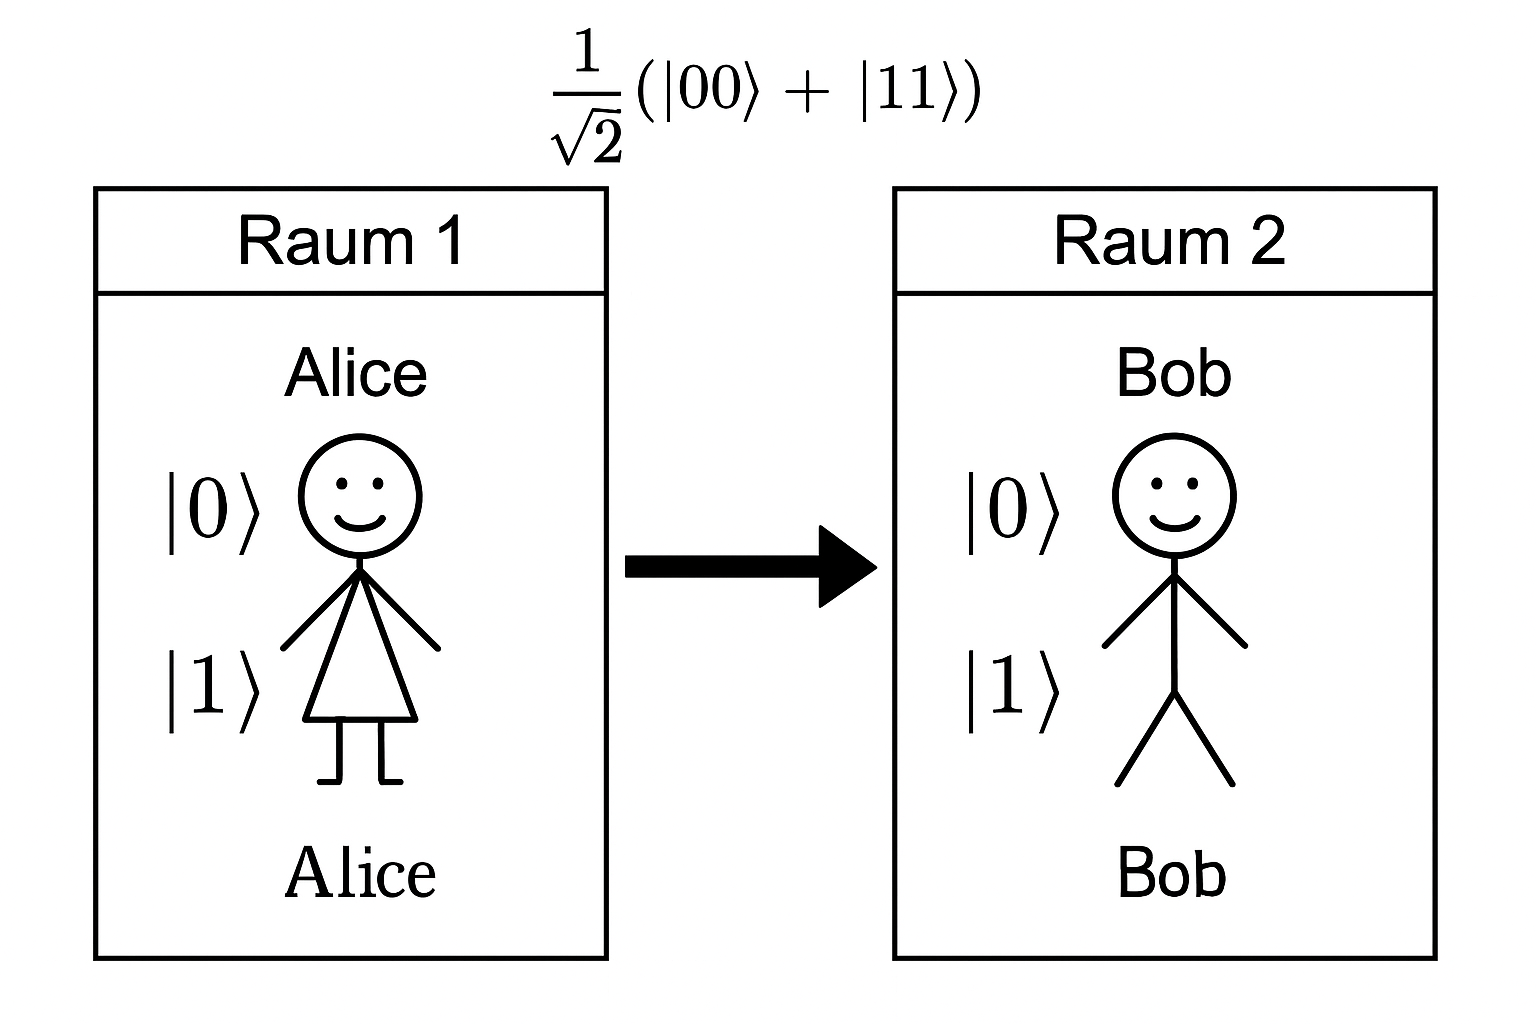
\includegraphics[width=0.5\textwidth]{images/quantum-information/Bell_Alice_Bob.png}
  \caption{Bell-Zustand: Alice und Bob}
\end{figure}



Genau darin zeigt sich der Informationsgehalt eines verschränkten Zustands: Die Information liegt nicht in einem einzelnen Qubit, sondern in ihrer gemeinsamen Beziehung. Diese Simulation macht das abstrakte Konzept der Quantenverschränkung greifbar und bietet einen intuitiven Zugang zu den Grundlagen der Quanteninformation. Es zeigt anschaulich, wie Quantencomputer fundamentale Prinzipien der Quantenmechanik sichtbar und messbar machen. 

\subsection{Bell-Zustand in der Praxis}

Bell-Zustände bilden das Fundament für viele Anwendungsfälle. Ein praktischer Anwendungsfall ist die Quantenkryptographie. Besonders bekannt ist insbesondere das sogenannte E91-Protokoll, welches auf dem Konzept der Quantenverschränkung beruht. Dabei erzeugt eine zentrale Quelle verschränkte Teilchenpaare und schickt je eines an zwei weit entfernte Personen – wie in unserem Beispiel etwa Alice und Bob. Wenn beide ihre Teilchen messen, erhalten sie stets perfekt korrelierte Ergebnisse. Dieser Effekt lässt sich nutzen, um einen gemeinsamen geheimen Schlüssel zu erzeugen. Ein Abhörversuch durch eine dritte Person würde diese Korrelation stören und könnte über einen Bell-Test erkannt werden. So kann mit Hilfe der Quantenmechanik sichergestellt werden, dass keine unbemerkte Informationsweitergabe stattgefunden hat – eine Grundlage für absolut sichere Kommunikation. (Vgl. \cite[S. 3841 f.]{kumar_state---art_2021})
\\


Quantenbasierte Protokolle stehen daher im Zentrum aktueller Forschung zur Quantenkryptographie und wurden bereits in ersten praktischen Experimenten erprobt. Besonders eindrucksvoll ist das Experiment mit dem chinesischen Micius-Satelliten: Er übermittelte verschränkte Photon-Bell-Paare an zwei Bodenstationen, die über eine Entfernung von rund 1200 Kilometern verteilt waren. Die gemessenen Korrelationen verletzten dabei deutlich die Bell-Ungleichung – ein klares Zeichen dafür, dass die beobachteten Effekte nicht durch klassische Physik erklärbar sind, sondern echte Quantenverschränkung vorliegt. Auf dieser Grundlage könnten über Kontinente hinweg geheime Schlüssel erzeugt und die Kommunikation verschlüsselt werden. (Vgl. \cite{ivezic_entanglement_2022})
\\


Ein zweiter praktischer Anwendungsfall des Bell-Zustands findet sich im Quantencomputing, genauer gesagt in der sogenannten Quantenteleportation. Dabei wird der Zustand eines Quantenbits (Qubit) von einem Ort zu einem anderen übertragen, ohne dass das Teilchen selbst physisch bewegt wird. Grundlage hierfür ist ein gemeinsam genutzter Bell-Zustand zwischen Sender (Alice) und Empfänger (Bob), der die nötige Verschränkung bereitstellt. Durch eine spezielle Messung auf Seiten von Alice und die Übermittlung zweier klassischer Bits kann Bob den ursprünglichen Zustand lokal wiederherstellen. (Vgl. \cite{bennett_teleporting_1993})
\\


Im Gegensatz zur Quantenkryptographie, bei der Sicherheit im Vordergrund steht, dient die Quanten-Teleportation der fehlerfreien Übertragung von Quanteninformation. Dies ist eine essenzielle Voraussetzung für die Vernetzung räumlich verteilter Quantencomputer. Sie gilt daher als Schlüsselfunktion zukünftiger Quantencomputer-Netzwerke, etwa im Rahmen eines „Quanteninternets“. (Vgl. \cite{ivezic_entanglement_2022}) Erste praktische Umsetzungen konnten dies bereits demonstrieren: 2017 gelang es ein Qubit über 1.400 km mit dem zuvor bereits erwähnten Satellit Micius erfolgreich zu teleportieren. (Vgl. \cite{ren_ground--satellite_2017})


\section{Zusammenfassung}
In diesem Kapitel wurden zentrale Konzepte der Quanteninformation eingeführt. Ausgangspunkt war das Qubit als quantenmechanisches Pendant zum klassischen Bit. Durch Superposition und komplexe Amplituden besitzt ein Qubit einen kontinuierlichen Zustandsraum, der auf der Bloch-Kugel visualisiert werden kann. In Kombination mit weiteren Qubits eröffnet sich durch Verschränkung ein exponentiell wachsender Zustandsraum, der die Basis für das sogenannte Quantenparallelismus bildet. Mit den Pauli- und Hadamard-Gattern sowie Mehr-Qubit-Gattern wie CNOT und SWAP wurden die grundlegenden Bausteine für Quantenoperationen vorgestellt. Aufbauend darauf wurden die ersten Quantenalgorithmen – insbesondere der Deutsch- und der Deutsch-Josza-Algorithmus – erläutert, die zeigen, wie Quantencomputer bestimmte Probleme effizienter lösen können als klassische Systeme. Darüber hinaus wurde die Bedeutung robuster Fehlerkorrekturmechanismen hervorgehoben, um die hohe Fehleranfälligkeit physikalischer Qubits auszugleichen. Schließlich wurde die Rolle der Quantenverschränkung für Kommunikation und Teleportation aufgezeigt. Anhand der Bell-Zustände wurde demonstriert, wie stark korrelierte Quantenpaare als Grundlage für Quantenkryptographie und verteilte Quantenberechnungen dienen. Insgesamt bietet dieses Kapitel eine Grundlage, um die Funktionsweise und das Potenzial von Quantencomputern zu verstehen und bereitet darauf vor, in den kommenden Kapiteln tiefer in Hardware, Software und konkrete Anwendungen einzutauchen.

\printbibliography


\begin{partbacktext}
\part{Quantencomputing}
%%\noindent Use the template \emph{part.tex} together with the document class SVMono (monograph-type books) or SVMult (edited books) to style your part title page and, if desired, a short introductory text (maximum one page) on its verso page.

\end{partbacktext}

%%%\motto{Use the template \emph{chapter.tex} to style the various elements of your chapter content.}
\chapter{Quantenhardware}
\label{hardware} % Always give a unique label
% use \chaptermark{}
% to alter or adjust the chapter heading in the running head

\chapterauthor{Daniel, Dennis, Jakob, Marc, Tom}

\abstract{some abstract}

\section{Die verschiedenen Quanten Hardwareplattformen}
\subsection{Einleitung und Unterschiede}
\subsection{Unterschied atomare und Festkörper Plattformen}

\section{Supraleitende Qubits}
\subsection{physikalisches Prinzip supraleitende qubits}
\subsection{Gatterimplementierung}
\subsection{Beispiele supraleitende Qubits}
\subsection{Herausforderungen supraleitende Qubits}

\section{Quantencomputer aus Ionenfallen-Qubits}
\subsection{Physikalisches Prinzip}
    - Zwei-Niveau-System
    - Photonen Manipulation (Elektromagnetisches Felder)
\subsection{Gatterimplementierung}
    - Wie funktioniert ein Logischer Gatter bei Ionenfallen-Quantencomputern?
    - Ein-Qubit-Gatter
    - Zwei-Qubit-Gatter
    - Cirac-Zoller-Gatter
    - Mølmer-Sørensen-Gatter
\subsection{Verwendungsbereiche und Merkmale der Ionenfallen-Qubits}
    - Stand der Technologie
    - Ionenfallen in Quantensimulation und Metrologie
    - Ionenfallen in Quantencomputer
    - Wie ist ein Ionenfallen Quantencomputer aufgebaut?
    - Wie und unter welchen Bedingungen wird ein Ionenfallen Quantencomputer benutzt/verwaltet?
\subsection{Herausforderungen und technische Limitationen}
    - Warum gibt es die aktuellen Probleme?
    - Skalierbarkeit
    - Gatterzeit
    - Potenzial
    - Ansätze zur Lösung aktueller Limitationen: z. B. Quantum Networking 

\section{Quantencomputer auf Basis diamantbasierter Qubits (NV-Zentren)}
\subsection{Physikalisches Prinzip}
    - Zwei-Niveau-System: Elektronenspins von Stickstoff-Fehlstellen (NV-Zentren) im Diamantgitter
    - Optische Kontrolle
    - Mikrowellensteuerung
    - Kernspins
\subsection{Gatterimplementierung}
    - Ein-Qubit-Gatter
    - Zwei-Qubit-Gatter
\subsection{Verwendungsbereiche und Merkmale der diamantbasierten Qubits}
    - Stand der Technologie
    - Anwendungen
    - Systemaufbau
    - Betriebsbedingungen
\subsection{Herausforderungen und technische Limitationen}
    - Warum gibt es die aktuellen Probleme?
    - Skalierbarkeit
    - Gatterzeiten:
    - Potenzial und Ansätze:



\section{Titel tbd}
\subsection{Photonische Quantencomputer}
\subsection{Halbleiterbasierte Qubits: Spin qubits}
\subsection{Neutralatom-Quantencomputer}
\subsection{Topologische Qubits}


\section{Quantencomputer-Architekturen und Vernetzung}
\subsection{Aufbau eines Quantenprozessors: Qubit-Array, Kopplungsmechanismen}
\subsection{Skalierungsstrategien: Modulare Systeme}
\subsection{Unterstützende Infrastruktur: Kryo-Elektronik, Hochfrequenzelektronik, Steuerungseinheiten, Filter gegen thermisches Rauschen}
\subsection{Erste Netzwerke: Konzepte des Quanteninternets (Architekturmodell), Quantenrepeater, Quantenrouter, Verschränkungsverteilung}

\section{Praxisbeispiel(e): Im Inneren eines IBM-Quantencomputers}

\subsection{Aufbaus eines kommerziellen Quantencomputers - IBM Q System One}
Beschreibung des Aufbaus eines kommerziellen Quantencomputers - IBM Q System One
Dieser Abschnitt beschreibt die physikalische Struktur eines typischen supraleitenden Quantencomputers. Im Fokus steht der Qubit-Chip, der auf einer stark heruntergekühlten Plattform montiert ist – einer sogenannten Verdünnungskühlstufe mit Temperaturen im Millikelvin-Bereich. Verschachtelte Abschirmungen und Vakuumkammern sorgen für eine minimale Störung durch Wärme, Strahlung oder elektromagnetische Einflüsse von außen.

\subsection{Foto-Illustration}
Foto-Illustration: Kaltes Verdünnungskryostat mit hängender Chip-Ebene (Gold-Coax-Kabel zu Qubits)
Hier wird mithilfe eines Bildes gezeigt, wie ein realer Kryostat aufgebaut ist, in dem der Qubit-Chip „hängt“. Die goldfarbenen Koaxialkabel, die an den Chip führen, dienen der Steuerung und Auslesung der Qubits mit hochfrequenten Mikrowellensignalen. Das Bild veranschaulicht die aufwendige technische Infrastruktur, die notwendig ist, um Quantenoperationen durchzuführen.

\subsection{Erläuterung eines einzelnen supraleitenden Qubits (Transmon)}
Erläuterung eines einzelnen supraleitenden Qubits (Transmon) und wie ein Zwei-Qubit-Gatter durch kapazitive Kopplung realisiert wird
Ein Transmon-Qubit ist ein spezieller supraleitender Schaltkreis, der zur Stabilisierung gegen Ladungsrauschen designt wurde. In diesem Teil wird erklärt, wie durch gezielte Mikrowellenpulse Zustände manipuliert und gelesen werden können. Zusätzlich wird gezeigt, wie zwei Transmon-Qubits über kapazitive Kopplung ein kontrolliertes Quantenlogikgatter bilden – ein zentrales Element zur Realisierung von Quantenalgorithmen.

\printbibliography

%%%\motto{Use the template \emph{chapter.tex} to style the various elements of your chapter content.}
\chapter{Grundlegende Quantenalgorithmen}
\label{basic_algorithms} % Always give a unique label
% use \chaptermark{}
% to alter or adjust the chapter heading in the running head

\chapterauthor{Vladimir Alyoshin, Gian-Luca Eberling}

\abstract*{some abstract}

\abstract{some abstract}

\section{Shor's Algorithmus zur Faktorisierung}

In der Informatik und insbesondere in der Kryptografie spielt die Sicherheit digitaler Kommunikation eine zentrale Rolle. Ein wesentliches Prinzip moderner Verschlüsselungsverfahren — etwa des RSA-Algorithmus — beruht auf der Annahme, dass die Zerlegung großer Zahlen in ihre Primfaktoren auf klassischen Computern mit exponentiellem Aufwand verbunden ist. Für ausreichend große Zahlen ist dieser Aufwand so gewaltig, dass selbst modernste Supercomputer über Jahre hinweg rechnen müssten, um einen privaten Schlüssel zu entschlüsseln.\\

Stellen wir uns vor, wir kennen lediglich eine große zusammengesetzte Zahl $N$, von der wir wissen, dass sie das Produkt zweier unbekannter Primzahlen $p$ und $q$ ist. Die klassische Faktorisierung würde in diesem Fall im schlimmsten Fall exponentiell viele Operationen erfordern. Genau hier setzt der Shor-Algorithmus an, der das Problem aus quantenmechanischer Sicht betrachtet.\\

Peter Shor entwickelte 1994 einen Algorithmus, der das Faktorisierungsproblem mithilfe eines Quantencomputers in polynomieller Zeit lösen kann — genauer gesagt in $\mathcal{O}((\log N)^3)$. Dies stellt eine exponentielle Beschleunigung gegenüber den besten bekannten klassischen Verfahren dar. Die zentrale Idee des Algorithmus liegt in der Reduktion des Faktorisierungsproblems auf das Periodenfindungsproblem, das sich durch Quanten-Phasenschätzung effizient lösen lässt.\\

Mit anderen Worten: Während klassische Computer für große $N$ praktisch keine Chance auf eine schnelle Faktorisierung haben, kann ein ausreichend großer Quantencomputer dieses Problem in überschaubarer Zeit lösen — mit drastischen Konsequenzen für die heute eingesetzten kryptografischen Verfahren.\\

Im Folgenden wird der Ablauf von Shors Algorithmus detailliert dargestellt und anhand eines konkreten Beispiels veranschaulicht. Dabei zeigen wir, wie Quantenregister, Quanten-Fourier-Transformation und die klassische Nachbearbeitung zusammenwirken, um die verborgenen Primfaktoren einer gegebenen Zahl zu enthüllen.\\


\subsection{Grundlagen: Primfaktorzerlegung und RSA}
Der RSA-Algorithmus basiert auf der Schwierigkeit, eine große Zahl \( N = pq \) zu faktorisieren. Shor’s Algorithmus bricht diese Sicherheit, indem er in polynomialer Zeit die Faktoren \( p \) und \( q \) bestimmt. Hat ein Angreifer Zugriff auf einen leistungsfähigen Quantencomputer, kann er aus dem öffentlichen Schlüssel die privaten Schlüsselparameter rekonstruieren. Shor's Algorithmus beschleunigt einen entscheidenen Schritt im klassischen Teil der Primfaktorzerlegung:

\begin{itemize}
  \item[a)] Wähle eine ganze Zahl \(x\) mit \(1 < x < N\).
  
  \item[b)] Berechne den größten gemeinsamen Teiler \(\gcd(x, N)\), z.\,B. mit dem Euklidischen Algorithmus.  
  \begin{itemize}
    \item Ist \(\gcd(x, N) \ne 1\), so gib \(\gcd(x, N)\) als nichttrivialen Teiler von \(N\) zurück und beende das Verfahren.
    \item Ist \(\gcd(x, N) = 1\), fahre mit Schritt c) fort.
  \end{itemize}
  
  \item[c)] Bestimme mit Hilfe des Quantenteils von Shor's Algorithmus die Ordnung \(r\) von \(x\) in der multiplikativen Gruppe \((\mathbb{Z}/N\mathbb{Z})^\times\), also das kleinste \(r \in \mathbb{N}\), sodass
  \[
  x^r \equiv 1 \mod N.
  \]
  
  \item[d)] Beginne erneut bei Schritt a), falls eine der folgenden Bedingungen zutrifft:
  \begin{itemize}
    \item \(r\) ist ungerade, oder
    \item \(x^{r/2} \equiv -1 \mod N\).
  \end{itemize}
  
  \item[e)] Berechne anschließend
  \[
  \gcd(x^{r/2} \pm 1, N)
  \]
  und gib mindestens einen der beiden Werte als nichttrivialen Teiler von \(N\) zurück.\\
  \[
  \]
  \textit{Hinweis:} Die so gefundenen Teiler müssen nicht direkt den gesuchten Primfaktoren \(p\) oder \(q\) entsprechen. Sie teilen jedoch \(N\) und können mit Hilfe des Euklidischen Algorithmus weiterverarbeitet werden, um auf die Primfaktoren zu schließen.
\end{itemize}


Shor's Algorithmus setzt bei Schritt c) ein und beschleunigt diesen massiv. Für einen klassischen Computer dauert es exponentiell lange diesen Schritt zu lösen. Dies zeigt, dass RSA bei hinreichend großen Quantencomputern als unsicher gelten muss.

Ziel ist es also, eine zusammengesetzte Zahl \( N = pq \) effizient zu faktorisieren. Um diese Faktorisierung zu beschleunigen nutzt Shor's Algorithmus die Periodizität der Funktion

\begin{definition}[Modulare Arithmetik] 
\[
f(a) = x^a \bmod N
\]
ist definiert als der Rest bei der Division von \(x^a\) durch \(N\).

\begin{itemize}
    \item \(x \in \mathbb{Z}\) ist eine Basiszahl, die kleiner als \(N\) und teilerfremd zu \(N\) sein sollte (d.h. \(\gcd(x, N) = 1\)).
    \item \(a \in \mathbb{N}_0\) ist der Exponent, eine natürliche Zahl (inkl. 0).
    \item \(N \in \mathbb{N}\) ist die zusammengesetzte Zahl, deren Primfaktorzerlegung wir bestimmen wollen.
    \item \(f(a)\) gibt den Rest an, wenn \(x^a\) durch \(N\) geteilt wird, also den Wert modulo \(N\).
\end{itemize}
\end{definition}
um mithilfe eines quantenmechanischen Verfahrens – konkret der Quanten-Phasenschätzung (QPE) – die Periode \( r \) dieser Funktion effizient zu bestimmen.

Im Algorithmus wird zunächst ein Superpositionszustand über viele Werte \( a \) erzeugt und anschließend durch eine unitäre Operation \( U_f \), die \( |a\rangle \mapsto |f(a)\rangle \) abbildet, mit den Funktionswerten moduliert.\\

Im nächsten Schritt erfolgt eine Quanten-Fouriertransformation (QFT) auf das Register, das die Werte von \( a \) enthält. Durch diese Fouriertransformation wird die Periodizität in der Amplitudenverteilung als charakteristische Spitzen (Peaks) sichtbar gemacht: Interferenzen zwischen den Zuständen führen dazu, dass bestimmte Frequenzanteile, die Vielfache von \( q/r \) (wobei \( q \) die Dimension des Registers ist) entsprechen, verstärkt werden, während andere ausgelöscht werden.\\

Je nach Konvention und Betrachtung kann man die QFT oder auch die inverse QFT (iQFT) verwenden; beide führen zur Hervorhebung der Periodizität im Zustandsraum, nur der genaue Ablauf der Transformation unterscheidet sich.\\

Nach der Fouriertransformation wird eine Messung durchgeführt, die mit hoher Wahrscheinlichkeit einen Wert \( c \) liefert, der näherungsweise in einem rationalen Verhältnis  
\[
\frac{c}{Q} \approx \frac{d}{r}
\]
zu \( r \) steht. Mithilfe der Kettenbruchentwicklung kann daraus die Periode \( r \) bestimmt werden.

Ist \( r \) bekannt und erfüllt sie bestimmte Voraussetzungen (z.B. \( r \) ist gerade und \( x^{r/2} \not\equiv -1 \bmod N \)), so lassen sich mit dem Euklidischen Algorithmus die Primfaktoren von \( N \) berechnen:  
\begin{definition}[Größter gemeinsamer Teiler (gcd)]
Der größte gemeinsame Teiler zweier Zahlen \(m, n \in \mathbb{N}\), bezeichnet als \(\gcd(m,n)\), ist die größte natürliche Zahl, die sowohl \(m\) als auch \(n\) ohne Rest teilt.\\

Im Kontext von Shor's Algorithmus verwenden wir
\[
\gcd\left(x^{r/2} \pm 1, N\right),
\]
wobei
\begin{itemize}
    \item \(x \in \mathbb{Z}\) eine Zahl ist, die teilerfremd zu \(N\) ist,
    \item \(r \in \mathbb{N}\) die Periode der Funktion \(f(a) = x^a \bmod N\) darstellt,
    \item \(N \in \mathbb{N}\) die zu faktorisierende zusammengesetzte Zahl ist,
    \item und \(x^{r/2} \pm 1\) eine Zahl ist, mit der wir durch die Berechnung des \(\gcd\) potenzielle Teiler von \(N\) finden.
\end{itemize}
\end{definition}

So nutzt Shor's Algorithmus die Quanteninterferenz und Fourier-Analyse, um versteckte Periodenstrukturen zu extrahieren und damit die Faktorisierung effizient zu ermöglichen.

\subsection{Aufbau des Shor Algorithmus}

Im folgenden Abschnitt werden wir alle notwendigen Methoden, Definitionen und Schritte beschreiben, die erforderlich sind, um den Shor-Algorithmus auszuführen. Dabei erklären wir Methode für Methode und wenden diese stets auf ein konkretes Beispiel an, um den Algorithmus möglichst präzise und anschaulich zu veranschaulichen. Anstelle einer sehr großen Zahl \( N \), wie sie in der Praxis als Schlüssel verwendet wird, wählen wir hier eine deutlich kleinere Zahl. \\

Der konkrete Fall, den wir betrachten, ist die Primfaktorzerlegung der Zahl \( N = 15 \). Natürlich kennen wir bereits die Primfaktoren \( 3 \) und \( 5 \). Es gilt somit \( N = q \cdot p \) mit \( q, p \in \mathbb{Z} \). \\

Zunächst muss festgelegt werden, wie groß der Hilbertraum \( Q = 2^n \) mit \( n \) Qubits sein muss, also die Gesamtanzahl aller Basiszustände des \( n \)-Qubit-Systems. Dies bestimmt, wie viele mögliche Zustände \( a \) betrachtet werden sollen. Dabei gilt die Bedingung
\[
2^n \geq N^2.
\]

Für unser Beispiel mit \( N = 15 \) ist \( N^2 = 225 \). Somit muss \( Q = 2^n \geq 225 \) gelten. Das entspricht mindestens \( n = 8 \) Qubits, da \( 2^8 = 256 \geq 225 \) ist. \\

Damit ergibt sich für das erste Register eine Größe von \( 8 \) Qubits. Das zweite Register benötigt
\[
m = \lceil \log_2(N) \rceil = \lceil \log_2(15) \rceil = 4
\]
Qubits.\\

Nun sind alle grundlegenden Variablen definiert und anhand eines konkreten Beispiels veranschaulicht. 
Bevor wir das Beispiel vollständig durchrechnen, formulieren wir zunächst die allgemeinen Schritte des Shor‑Algorithmus:

\begin{enumerate}
    \item \textbf{Initialisierung in einen Superpositionszustand:} 
    Die erste Operation besteht darin, zwei Quantenregister entsprechend der berechneten Qubit-Größen als Eingabe und Ausgaberegister zu erzeugen, welche sich alle in den Basiszuständen befinden, also mit der gleichen Wahrscheinlichkeit auftreten:
\[
\ket{\psi_0} = \ket{0}^{\otimes n} \otimes \ket{0}^{\otimes m}
\]
    Die \textit{Gleichverteilung} wird dadurch erreicht, dass die Amplituden aller Zustände gleich sind. Wenn das System anfangs im Zustand $\ket{0}^{\otimes n}$ ist (alle Qubits auf 0), dann erzeugen wir durch Anwendung der Hadamard-Transformation auf jedes Qubit die Superposition - aber nur auf das erste Register:

$$
\ket{\psi_1} = \frac{1}{\sqrt{Q}} \sum_{a=0}^{Q-1} \ket{a}
$$
Dabei ist:
  \begin{itemize}
    \item \( n \): Anzahl der Qubits im ersten Register.
    \item \( Q = 2^n \): Anzahl der möglichen Zustände im ersten Register
    \item \( x \): Laufvariable über alle Basiszustände von \( \ket{0} \) bis \( \ket{Q-1} \).
    \item \( 1 \): Anfangszustand des zweiten Registers, auf das später die modulare Exponentiation angewendet wird.
  \end{itemize}

  Durch die Hadamard-Gates wird das Register in eine Superposition gebracht, in der alle \( Q \) Basiszustände gleichwahrscheinlich sind. Diese Superposition ist notwendig, um später durch die Phaseninterferenz Information über die Periode der Funktion zu extrahieren.\\
 \item \textbf{Unitäre Funktion anwenden} 
\[
U_f \colon |a\rangle|1\rangle \mapsto |a\rangle|x^a \bmod N\rangle
\]
\begin{itemize}
    \item \textbf{\( a \)}: Wert im ersten Register (Index der Superposition), typischerweise \( a \in \{0, 1, \dotsc, Q-1\} \) mit \( Q = 2^n \), wobei \( n \) die Anzahl der Qubits im ersten Register ist.
    \item \textbf{\( x \)}: Eine zufällig gewählte ganze Zahl mit \( 1 < x < N \), die zu \( N \) teilerfremd ist.
    \item \textbf{\( N \)}: Die zusammengesetzte Zahl, deren Primfaktoren bestimmt werden sollen.
    \item \textbf{\( U_f \)}: Eine unitäre Transformation, die auf beiden Registern wirkt. Sie berechnet im zweiten Register die Funktion \( f(a) = x^a \bmod N \), wobei das erste Register \( |a\rangle \) als Steuerregister dient.
\end{itemize}

Nach Anwendung von \( U_f \) ergibt sich der verschränkte Zustand
\[
\ket{\psi_2} = \frac{1}{\sqrt{Q}} \sum_{a=0}^{Q-1} \ket{a} \otimes \ket{x^a \bmod N}
\]
Dieser Zustand ist eine Superposition über alle möglichen Paare \( (a, f(a)) \), wobei \( f(a) = x^a \bmod N \) die periodische Struktur trägt, die später durch die Quanten-Fourier-Transformation im ersten Register erkennbar gemacht wird.\\

\item \textbf{Quanten-Fourier-Transformation (QFT) auf das erste Register anwenden}

\noindent Die Quanten-Fourier-Transformation wird nun auf das erste Register angewendet. Diese transformiert den Zustand \( |a\rangle \) gemäß:

\[
\mathrm{QFT}(|a\rangle) = \frac{1}{\sqrt{Q}} \sum_{c=0}^{Q-1} e^{2\pi i \frac{a c}{Q}} |c\rangle
\]

\begin{itemize}
    \item \( Q = 2^n \): Anzahl der Basiszustände im ersten Register.
    \item \( a \): Index im ersten Register vor der QFT.
    \item \( c \): Index nach der Fouriertransformation – potenzieller Messwert.
\end{itemize}

\noindent Daraus ergibt sich der Gesamtzustand nach Anwendung der QFT:
\[
\ket{\psi_3} = \frac{1}{Q} \sum_{a=0}^{Q-1} \sum_{c=0}^{Q-1} e^{2\pi i \frac{a c}{Q}} \ket{c} \otimes \ket{x^a \bmod N}
\]

\noindent In der Quanten-Fourier-Transformation entsteht in jedem Summand der Ausdruck
\[
e^{2\pi i \frac{a c}{Q}},
\]
der eine komplexe \(Phasenrotation\) beschreibt.

\begin{itemize}
    \item \textbf{\( a \)}: Index des ursprünglichen Zustands im Superpositionsregister.
    \item \textbf{\( c \)}: Index des Zielzustands nach der Fouriertransformation.
    \item \textbf{\( Q \)}: Anzahl möglicher Zustände im Register (meist \( Q = 2^n \)).
\end{itemize}

\noindent Diese Phasenfaktoren lassen sich mit Hilfe der Euler-Formel interpretieren:
\[
e^{2\pi i \frac{a c}{Q}} = \cos\left(2\pi \frac{a c}{Q}\right) + i \cdot \sin\left(2\pi \frac{a c}{Q}\right)
\]

\noindent Es handelt sich also um eine \(Rotation\) \(im\) \(komplexen\) \(Raum\) – die komplexe Zahl liegt auf dem Einheitskreis und rotiert je nach Kombination von \( a \) und \( c \) um einen bestimmten Winkel. Dadurch ergibt sich:

\begin{itemize}
    \item Jeder Zustand \( |a\rangle \) trägt mit einer anderen Phase zur Superposition bei.
    \item Bei periodischer Struktur der Funktion \( f(a) = x^a \bmod N \) interferieren die komplexen Phasen systematisch.
    \item Dies führt dazu, dass bei der Messung des ersten Registers nur bestimmte Werte \( c \) mit hoher Wahrscheinlichkeit auftreten – die sogenannten \(Fourier-Peaks\).
    \item Andere Zustände löschen sich durch destruktive Interferenz aus.
\end{itemize}

\noindent Genau diese Interferenzstruktur erlaubt es, verborgene Perioden zu extrahieren – und damit den entscheidenden quantenmechanischen Vorteil zur Faktorisierung auszunutzen.\\

\item \textbf{Periodenbestimmung durch Kettenbruchentwicklung}

\noindent Nach der Fouriertransformation wird eine Messung durchgeführt, die mit hoher Wahrscheinlichkeit einen Wert \( c \) liefert, der näherungsweise in einem rationalen Verhältnis steht:
\[
\frac{c}{Q} \approx \frac{d}{r}
\]

\begin{itemize}
    \item \( c \): Messwert aus dem ersten Register nach Anwendung der QFT.
    \item \( Q \): Anzahl möglicher Zustände im ersten Register (typischerweise \( Q = 2^n \), mit \( Q > N^2 \)).
    \item \( d \): unbekannter ganzzahliger Zähler.
    \item \( r \): die Periode der Funktion \( f(a) = x^a \bmod N \), die bestimmt werden soll.
\end{itemize}

\noindent Ziel ist es, aus dem gemessenen Bruch \( \frac{c}{Q} \) eine möglichst genaue Näherung \( \frac{d}{r} \) zu finden, wobei \( r \) möglichst klein ist. Dies gelingt über die sogenannte \(Kettenbruchentwicklung\):

\begin{enumerate}
    \item Entwickle den Bruch \( \frac{c}{Q} \) in einen Kettenbruch.
    \item Brich die Entwicklung an mehreren Stellen ab und bilde die entsprechenden Konvergenten \( \frac{d_i}{r_i} \).
    \item Prüfe für jedes \( r_i \), ob \( x^{r_i} \equiv 1 \mod N \) gilt.
    \item Der kleinste passende \( r_i \) ist dann mit hoher Wahrscheinlichkeit die gesuchte Periode \( r \).
\end{enumerate}

\noindent Sobald die Periode \( r \) gefunden wurde, kann man im nächsten Schritt durch Berechnung des größten gemeinsamen Teilers (siehe \texttt{gcd}-Definition) mögliche Faktoren von \( N \) bestimmen:
\[
\gcd(x^{r/2} \pm 1, N)
\]

\noindent Damit ist der zentrale algorithmische Teil von Shor abgeschlossen – die restlichen Schritte sind rein klassisch.\\
\end{enumerate}

\noindent
Alle Operationen lassen sich im wesentlichen wie folgt zusammenfassen: Zunächst erfolgt die Initialisierung von zwei Quantenregistern, wobei das erste in eine Superposition aller möglichen Werte gebracht wird und das zweite den Ausgangszustand \( |1\rangle \) erhält. Durch Anwendung der unitären Funktion \( U_f \) wird eine Kopplung zwischen den Registern hergestellt, die die periodische Struktur der Funktion \( f(a) = x^a \bmod N \) abbildet. Anschließend findet die Quanten-Fourier-Transformation (QFT) auf dem ersten Register statt, wodurch mittels Interferenzinformation über die Periode \( r \) gewonnen wird. Die Messung des ersten Registers liefert eine Näherung an einen Bruch \( d/r \), aus dem mit der Kettenbruchentwicklung die Periode bestimmt wird. Auf Basis dieser Periode können die Teiler von \( N \) berechnet werden. \\

\noindent Die Operationen des Shor's Algorithmus zur Faktorisierung lassen sich wie folgt darstellen:

\begin{algorithm}[H] % <-- [H] erzwingt Platzierung an dieser Stelle
\caption{Shor's Algorithmus zur Faktorisierung einer Zahl \( N \)}
\label{algorithm:shor}
\begin{algorithmic}[1]
\Require Eine zusammengesetzte Zahl \( N \) aus zwei unbekannten Primzahlen \( p \) und \( q \)
\Ensure Ein nicht-trivialer Teiler von \( N \)
\State Wähle zufällig eine ganze Zahl \( x \) mit \( 1 < x < N \)
\If{\( \gcd(x, N) \neq 1 \)}
    \State \Return \( \gcd(x, N) \) \Comment{Zufällig gewähltes \( x \) war schon ein Teiler}
\EndIf
\State Bestimme die Periode \( r \) der Funktion \( f(x) = x^a \bmod N \) mittels Quanten-Phasenschätzung:
\State Initialisiere zwei Register: Eins mit Superposition aller \( x \), eins mit Zustand \( |1\rangle \)
\State Wende die unitäre Operation \( U_f \colon |a\rangle|1\rangle \mapsto |a\rangle|x^a \bmod N\rangle \) an
\State Wende die Quanten-Fourier-Transformation (QFT) auf das erste Register an
\State Miss das erste Register → erhalte Näherung \( d/r \)
\State Berechne \( r \) durch Kettenbruchentwicklung
\If{\( r \) ungerade oder \( x^{r/2} \equiv -1 \bmod N \)}
    \State \Return \textbf{Fehlschlag, wähle anderes \( a \)} und wiederhole
\EndIf
\State Berechne \( \gcd(x^{r/2} \pm 1, N) \)
\State \Return Einer der berechneten Teiler ist eine Primzahl \( p \) oder \( q \)
\end{algorithmic}
\end{algorithm}

\subsection{Rechenbeispiel – Shor's-Algorithmus}

Im folgenden Abschnitt wird das zu Beginn beschriebene Beispiel \( N = 15 \) vollständig durchgerechnet:

Wir wählen \( N = 15 \) und \( x = 2 \). Für den Algorithmus benötigen wir ein erstes Register mit mindestens \( n = 8 \) Qubits, sodass \( Q = 2^n = 256 > N^2 = 225 \) gilt. Das zweite Register benötigt nur \( m = \lceil \log_2 N \rceil = 4 \) Qubits, da es die Werte von \( f(a) = 2^a \bmod 15 \) aufnehmen muss.

\begin{enumerate}
    \item \textbf{Initialisierung in einen Superpositionszustand} \\
    Der Anfangszustand ist:

    \[
    \ket{\psi_0} = \ket{0}^{\otimes 8} \otimes \ket{0}^{\otimes 4}
    \]

    Nach Anwendung von Hadamard-Gattern auf alle 8 Qubits des ersten Registers entsteht die Gleichverteilung (Superposition) über alle \( Q = 256 \) Zustände:

    \[
    \ket{\psi_1} = \frac{1}{\sqrt{256}} \sum_{a=0}^{255} \ket{a} \otimes \ket{0}
    \]

    Diese Superposition ermöglicht es, alle Werte \( a \) gleichzeitig zu verarbeiten.\\

    \item \textbf{Anwendung der unitären Funktion \( U_f \)} \\

    Die Funktion \( f(a) = 2^a \bmod 15 \) wird auf das zweite Register angewandt, ohne das erste Register zu verändern. Die Transformation lautet:

    \[
    U_f: \ket{a} \ket{0} \mapsto \ket{a} \ket{2^a \bmod 15}
    \]

    Der Zustand nach Anwendung von \( U_f \) ist:

    \[
    \ket{\psi_2} = \frac{1}{\sqrt{256}} \sum_{a=0}^{255} \ket{a} \ket{2^a \bmod 15}
    \]

    Um das Verhalten der Funktion \( f(a) = 2^a \bmod 15 \) besser zu verstehen, berechnen wir die ersten Funktionswerte:

    \[
    \begin{array}{c|c}
    a & f(a) = 2^a \bmod 15 \\
    \hline
    0 & 1 \\
    1 & 2 \\
    2 & 4 \\
    3 & 8 \\
    4 & 1 \\
    5 & 2 \\
    6 & 4 \\
    7 & 8 \\
    8 & 1 \\
    \end{array}
    \]

    Wir erkennen: Die Funktionswerte wiederholen sich mit einer Periode \( r = 4 \), also \( 2^4 \bmod 15 = 1 \).
    \begin{figure}[H]
    \centering
    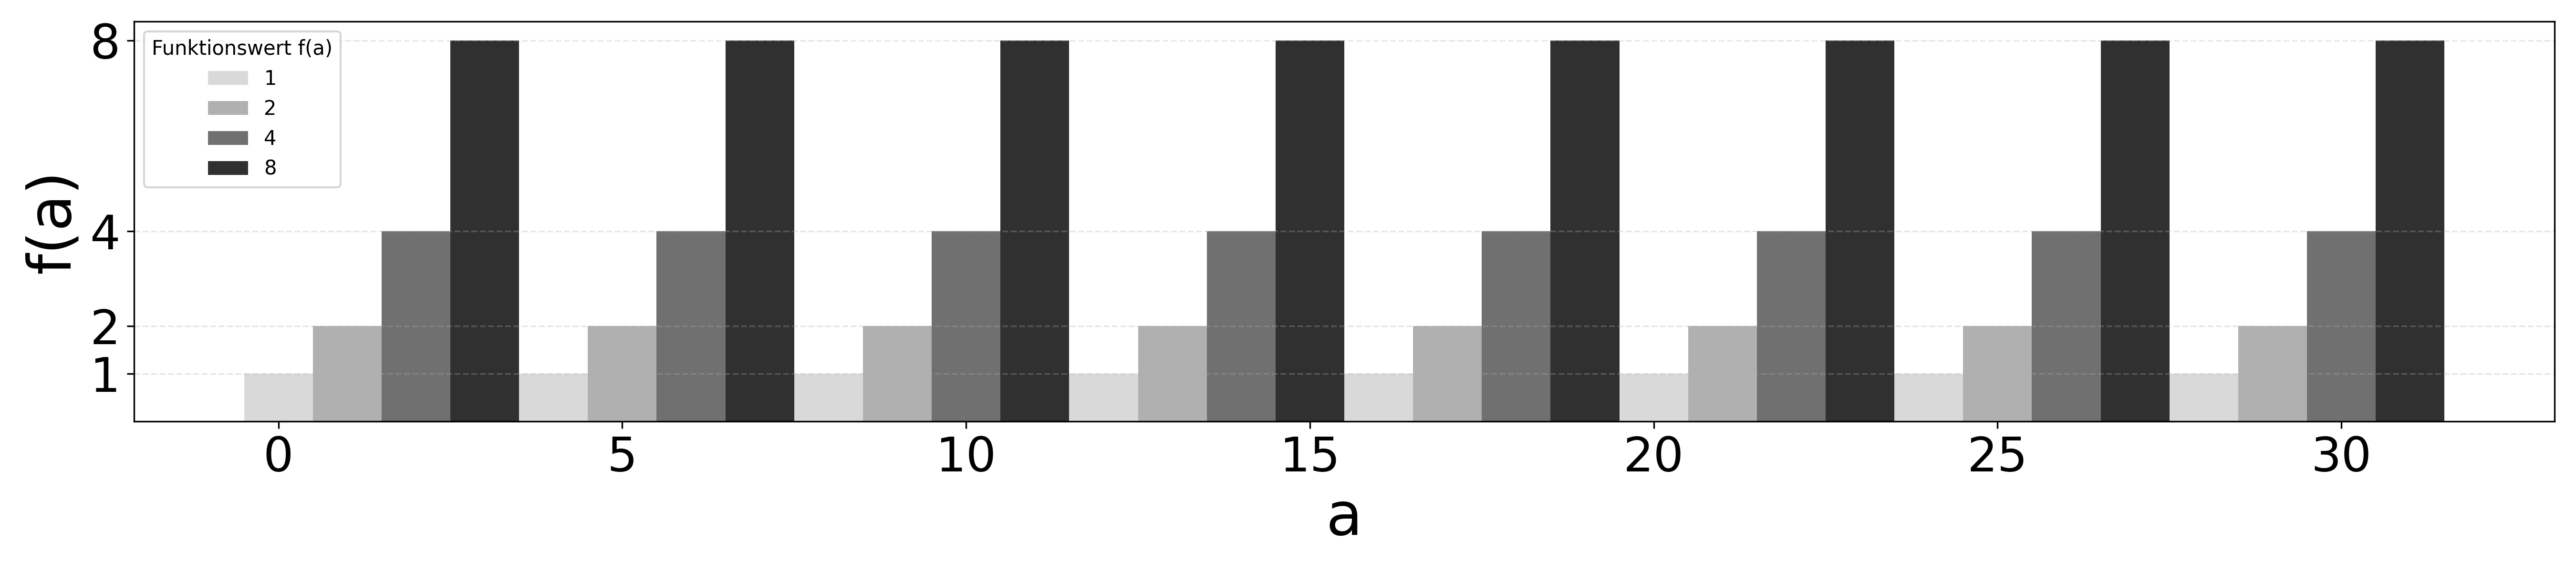
\includegraphics[width=1\textwidth,height=6cm,keepaspectratio]{images/basic-algorithms/shor_mod15_frequenz_graustufen.png}
    \caption{Visualisierung von $f(a) = 2^a \bmod 15$ mit Periode $r$ = 4}
    \label{fig:Visualisierung von $f(a) = 2^a \bmod 15$ mit Periode $r$ = 4}
\end{figure}

    Der verschränkte Zustand besteht also aus Gruppen gleicher Ausgabewerte:

    \[
    \ket{\psi_2} = \frac{1}{\sqrt{256}} \left( \ket{0} \ket{1} + \ket{4} \ket{1} + \ket{8} \ket{1} + \dots + \ket{252} \ket{1} + \dots \right) + \dots
    \]

    Dabei erscheinen alle \( a \)-Werte, die den gleichen Funktionswert liefern, gemeinsam mit dem jeweiligen \( \ket{f(a)} \).\\

    \item \textbf{Quanten-Fourier-Transformation (QFT)} \\

    Jetzt wenden wir auf das erste Register die QFT an. Die QFT transformiert die Basiszustände wie folgt:

    \[
    \mathrm{QFT}(\ket{a}) = \frac{1}{\sqrt{256}} \sum_{c=0}^{255} e^{2\pi i a c / 256} \ket{c}
    \]

    Die QFT wirkt linear auf jeden Summanden, sodass sich der Gesamtzustand ergibt als:

    \[
    \ket{\psi_3} = \frac{1}{256} \sum_{a=0}^{255} \sum_{c=0}^{255} e^{2\pi i a c / 256} \ket{c} \ket{2^a \bmod 15}
    \]

    Die Periode \( r = 4 \) der Funktion \( f(a) = 2^a \bmod 15 \) sorgt dafür, dass bei der Messung des ersten Registers besonders häufig Vielfache von \( \frac{Q}{r} = \frac{256}{4} = 64 \) auftreten. Erwartbare Messwerte sind also \( c \in \{0, 64, 128, 192\} \).\\

    \item \textbf{Messung und Kettenbruchentwicklung} \\

    Nehmen wir an, bei der Messung des ersten Registers erhalten wir \( c = 64 \). Daraus ergibt sich:

    \[
    \frac{c}{Q} = \frac{64}{256} = \frac{1}{4}
    \]

    Dies ist in diesem Beispiel bereits vollständig gekürzt – in der Praxis verläuft dies jedoch nicht immer so glatt. Über die Kettenbruchentwicklung von \( \frac{1}{4} \) folgt sofort \( r = 4 \) als vermutete Periode.\\

    \item \textbf{Faktoren berechnen} \\

    Mit der gefundenen Periode \( r = 4 \) testen wir, ob sich damit die Faktoren von \( N = 15 \) bestimmen lassen. Dafür prüfen wir:

\[
\gcd(x^{r/2} - 1, N) = \gcd(2^2 - 1, 15) = \gcd(3, 15) = 3
\]
\[
\gcd(x^{r/2} + 1, N) = \gcd(2^2 + 1, 15) = \gcd(5, 15) = 5
\]

    Wir erhalten die nicht-trivialen Faktoren 3 und 5 von \( N = 15 \). Die Faktorisierung ist damit erfolgreich abgeschlossen.\\

\textit{Hinweis:} Dass hier direkt beide Primfaktoren von \( N \) ermittelt werden, ist ein Glücksfall dieses kleinen Beispiels. In realistischen Anwendungen des Shor-Algorithmus ist es üblich, dass einer oder beide der berechneten Werte lediglich einen gemeinsamen Teiler mit dem ursprünglichen \( N \) ergeben. Diese Teiler führen aber dennoch – eventuell nach mehreren Wiederholungen von Euklids Algorithmus– zuverlässig zur vollständigen Faktorisierung, da der Algorithmus mit hoher Wahrscheinlichkeit mindestens einen nicht-trivialen Teiler liefert.

\end{enumerate}

Der Shor-Algorithmus zeigt, wie Quantencomputer periodische Strukturen in Funktionen aufdecken können, die klassisch nur mit exponentiellem Aufwand zu finden wären. Die Kombination aus Quanten-Phasenabschätzung, Fourier-Transformation und Kettenbruchentwicklung ermöglicht eine effiziente Faktorisierung großer Zahlen – ein fundamentaler Angriff auf die Sicherheit klassischer Verschlüsselung.\\

Damit stellt der Shor-Algorithmus einen Meilenstein in der Quanteninformatik dar: Er demonstriert das Potenzial quantenmechanischer Algorithmen, bestimmte Probleme deutlich schneller zu lösen als klassische Verfahren. Besonders betroffen ist dabei die auf der Faktorisierung großer Zahlen basierende Kryptographie, wie etwa RSA, deren Sicherheitsversprechen durch die Existenz effizienter Quantenalgorithmen grundlegend in Frage gestellt wird.\\

Obwohl praktische Quantencomputer mit ausreichend vielen stabilen Qubits derzeit noch in der Entwicklung sind, verdeutlicht Shors Algorithmus bereits jetzt die Notwendigkeit, langfristig auf quantensichere Verschlüsselungsverfahren umzusteigen. Die theoretischen Grundlagen, wie sie in diesem Kapitel erarbeitet wurden, schaffen ein tiefes Verständnis für die Funktionsweise und Tragweite dieses Algorithmus und bilden die Basis für weitere Forschung im Bereich der Quantenalgorithmen und der Post-Quanten-Kryptographie.

\section{Grover-Algorithmus: Quantum-Suche}
\label{sec:grover-algorithm}
In der Informatik zählt die Datenverarbeitung zu den gefragtesten Aufgaben. In der heutigen Zeit ist die Möglichkeit, große Datenmengen zu durchsuchen — insbesondere unstrukturierte Daten — ein wesentlicher Aspekt der Datenanalyse. Um dies zu veranschaulichen, betrachten wir folgendes Beispiel:\\ 

Angenommen, wir möchten einen bestimmten Kunden in der Datenbank eines Online-Shops finden (unter der Annahme, dass die Datenbank nicht indexiert ist). Bei Verwendung eines klassischen Computers benötigen wir im schlechtesten Fall $N$ Iterationen, wobei $N$ die Anzahl der Zeilen in der Tabelle darstellt. Im durchschnittlichen Fall sind etwa $N/2$ Operationen erforderlich. Das bedeutet, dass alle Elemente der Tabelle durchlaufen werden müssen, sofern uns die genaue Position des gesuchten Kunden nicht bekannt ist — bis dieser schließlich gefunden wird.\\

Wenn jedoch unsere Datenbank auf Quantenberechnungen basiert, können wir Quanten-Suchalgorithmen wie den Grover-Algorithmus einsetzen. In diesem Fall lässt sich das gesuchte Element mit etwa $\sqrt{N}$ Operationen finden. Zwar führt dieser Algorithmus nicht zu einer exponentiellen Beschleunigung der Suche und muss häufig mehrfach iterativ aufgerufen werden, dennoch stellt die quadratische Laufzeit bereits eine bedeutende Optimierung dar.

\subsection{Grundlagen: Unstrukturiertes Suchproblem}
Bevor wir uns dem Grover-Algorithmus zuwenden, betrachten wir folgendes Beispiel: Stellen wir uns vor, auf dem Tisch liegen vier Spielkarten verdeckt. Eine dieser vier Karten ist die Pik-Dame, und unsere Aufgabe besteht darin, sie zu finden. Wie viele Karten müssen wir im Durchschnitt aufdecken, um die Pik-Dame zu identifizieren? Im besten Fall finden wir die gesuchte Karte bereits beim ersten Versuch. Im schlechtesten Fall müssen wir drei Karten umdrehen — wenn keine von ihnen die Pik-Dame ist, dann bleibt nur noch die vierte, nicht aufgedeckte Karte als einzig mögliche Lösung. Im Durchschnitt müssen wir 2{,}25 Karten aufdecken, um die Pik-Dame zu finden.\\

Formulieren wir nun das Beispiel um: Anstelle von Spielkarten betrachten wir eine binäre Reihenfolge natürlicher Zahlen — nämlich $00$, $01$, $10$ und $11$. Nehmen wir an, die Pik-Dame entspricht dabei der Zahl $11$. Wir definieren eine Funktion $f$, die den Wert $1$ zurückgibt, wenn das Eingabemuster $11$ ist, und $0$ in allen anderen Fällen. Somit lässt sich das Problem wie folgt formal ausdrücken:

\begin{definition}[Unstrukturiertes Suchproblem]
Sei $f\colon \{0, 1\}^n \rightarrow \{0, 1\}$ eine abstrakte Funktion mit $f(x) \in \{0, 1\}$. Gesucht ist ein Wert $x$, sodass $f(x) = 1$, falls ein solcher Wert existiert; andernfalls soll das Ergebnis $0$ sein.(\cite{montanaro_quantum_2016})
\end{definition}

Die Komplexität des unstrukturierten Suchproblems ergibt sich daraus, wie viele Iterationen der Funktion erforderlich sind, um das gesuchte Element zu finden. Wir benötigen im schlechtesten Fall $N - 1$ Funktionsauswertungen, wobei $N = 2^n$ gilt. Auf diese Weise prüfen wir alle möglichen Eingaben. Ähnlich wie im Beispiel mit den Karten entspricht $N$ dem letzten Element, vorausgesetzt, die vorherigen wurden bereits geprüft. Der Grover-Algorithmus kann dieses Problem jedoch deutlich schneller lösen und erreicht dabei eine quadratische Laufzeitverbesserung.\\

Jedoch repliziert der Grover-Algorithmus noch ein Suchproblem. Wie wir im Beispiel mit den Spielkarten gesehen haben, müssen wir Karte für Karte umdrehen, um zu prüfen, ob es die gesuchte Karte ist oder nicht. Dieser Prozess ist iterativ und wird durch das \textit{heuristische Suchproblem} beschrieben (\cite{montanaro_quantum_2016}):

\begin{definition}[Heuristisches Suchproblem]
Gegeben sei die Möglichkeit, einen probabilistischen „Rate“-Algorithmus \( A \) auszuführen, und eine „Prüf“-Funktion \( f \), sodass

\[
\Pr\left[ A \text{ gibt } w \text{ aus, sodass } f(w) = 1 \right] = \varepsilon,
\]
\end{definition}

Eine Möglichkeit, das heuristische Suchproblem klassisch zu lösen, besteht darin, den Algorithmus \( A \) wiederholt auszuführen und jedes Ergebnis mit der Funktion \( f \) zu überprüfen. Dies führt zu durchschnittlich \( O\left(\frac{1}{\varepsilon}\right) \) Auswertungen von \( f \). In der nächsten Sektion werden wir sehen, wie der Grover-Algorithmus dieses Verfahren implementiert.

\subsection{Aufbau des Grover Algorithmus}

Um den Grover-Algorithmus vollständig zu verstehen, ist es wichtig, zunächst die grundlegenden Quantenoperationen zu begreifen. Lov Grover führte die folgende Definition für eine bestimmte Klasse von Operationen ein.\cite[1-2]{zotero-1211}

\begin{definition}[Unitäre Operationen]
Quantenmechanische Operationen, die in kontrollierter Weise ausgeführt werden können, sind \emph{unitäre Operationen}, welche in jedem Schritt auf eine kleine Anzahl von Qubits wirken.
\end{definition}

Der Grover-Algorithmus basiert auf einer Folge solcher unitären Operationen, die auf einen reinen Anfangszustand angewendet werden. Diese Operationen dienen dazu, die Wahrscheinlichkeit des gesuchten Ergebnisses zu verstärken. Am Ende des Algorithmus erfolgt eine Messung des resultierenden Zustands. Diese Messung projiziert das überlagerte Quantensystem auf einen klassischen Zustand, der mit hoher Wahrscheinlichkeit die Lösung des zugrunde liegenden Suchproblems enthält.\\

Lov Grover definierte die folgenden unitären Operationen (\cite{zotero-1211}) als zentrale Bestandteile seines Algorithmus:

\begin{enumerate}
    \item \textbf{Initialisierung in einen Superpositionszustand (\ref{sec: Superposition}):} 
    Die erste Operation besteht darin, ein Quantenregister mit $n$ Qubits (entsprechend $N = 2^{n}$ möglichen Zuständen) in einen Zustand zu überführen, in dem alle Basiszustände mit der gleichen Wahrscheinlichkeit auftreten – also eine \textit{Gleichverteilung}. Die \textit{Gleichverteilung} wird dadurch erreicht, dass die Amplituden aller Zustände gleich sind. Wenn das System anfangs im Zustand $\ket{0}^{\otimes n}$ ist (alle Qubits auf 0), dann erzeugen wir durch Anwendung der Hadamard-Transformation auf jedes Qubit die Superposition:

$$
\ket{\psi_0} = \frac{1}{\sqrt{N}} \sum_{x=0}^{N-1} \ket{x}
$$

Dies ist die gleichmäßige Superposition über alle möglichen Zustände $\ket{x}$ mit $x \in {0, \ldots, N-1}$.\\
    \item \textbf{Walsch-Hadamard Transformation}: Hadamard Transformation ist eine wichtige Quantummechanische Operation, die durch eine Operation $H$ definiert ist.(\ref{subsubsec:hadamard_gatter}) Diese Operation wird auf ein einzelnes Qubit angewendet und wird durch die folgende Matrix dargestellt:
    $$
H = \frac{1}{\sqrt{2}} \begin{pmatrix}
1 & 1 \\
1 & -1 \\
\end{pmatrix}
$$
Ein Qubit im Zustand \( \lvert 0 \rangle \) wird in eine Superposition der beiden Zustände überführt: \( \left( \frac{1}{\sqrt{2}}, \frac{1}{\sqrt{2}} \right) \). Die Wirkung auf die Basiszustände ist:

$$
H\ket{0} = \frac{1}{\sqrt{2}}(\ket{0} + \ket{1}), \quad H\ket{1} = \frac{1}{\sqrt{2}}(\ket{0} - \ket{1})
$$
Wendet man $H$ auf jedes der $n$ Qubits an, so entsteht eine Transformation $H^{\otimes n}$, die eine $2^n \times 2^n$-Matrix darstellt.
Besonders interessant ist, dass das Vorzeichen (also die Phase) des Amplitudenwertes nach der Hadamard-Transformation vom Skalarprodukt der Eingabe- und Ausgabebits abhängt:

$$
\text{Vorzeichen} = (-1)^{x \cdot y}
$$

Dabei ist $x \cdot y$ das bitweise Skalarprodukt der $n$-Bit-Binärzahlen $x$ und $y$.\\

    \item \textbf{Selektive Phasenrotation:} Die dritte elementare Operation ist die selektive Phasenrotation der Amplitude in bestimmten Zuständen.(\cite{zotero-1211}) Die Transformation, die dies für ein Zwei-Zustands-System beschreibt, hat die Form:

    $$
R = \begin{pmatrix}
e^{i\phi_1} & 0 \\
0 & e^{i\phi_2}
\end{pmatrix}
$$

wobei \( \phi \) eine beliebige reelle Zahl ist. Es ist zu beachten, dass – im Gegensatz zur Walsh-Hadamard-Transformation und anderen Zustandsübergangsmatrizen – die Wahrscheinlichkeit in jedem Zustand gleich bleibt, da das Quadrat des Betrags der Amplitude in jedem Zustand unverändert bleibt.
Im Grover-Algorithmus wird die Phasenrotation speziell dafür genutzt, um den gesuchten Zustand $\ket{x\_{\text{target}}}$ zu markieren, indem dessen Amplitude mit $-1$ multipliziert wird, während alle anderen Zustände unverändert bleiben:

$$
\ket{x} \mapsto 
\begin{cases}
- \ket{x}, & \text{wenn } x = x_{\text{target}} \\
\ket{x}, & \text{sonst}
\end{cases}
$$

\end{enumerate}

Zusammenfassend lässt sich einfach sagen: Der Grover-Algorithmus verwendet diese Operationen, um pro Iteration zwei Schritte auszuführen:
\begin{enumerate}
  \item Vorzeichenumkehr der Wahrscheinlichkeitsamplitude des gesuchten Elements.
  \item Verstärkung der Wahrscheinlichkeitsamplitude.
\end{enumerate}

Mit dem Verständnis der oben genannten unitären Operationen lässt sich der Grover-Algorithmus durch die folgenden Schritte beschreiben:

\begin{algorithm}[H]
\label{alg:grover}
\caption{Grover-Suchalgorithmus}
\begin{algorithmic}[1]
\State Erzeuge ein Register aus \( n \) Qubits im Zustand \( \ket{0}^{\otimes n} \).
\State Wende die Hadamard-Operation \( H \) auf jedes Qubit an, um eine Superposition zu erzeugen.
\Repeat
  \State\textbf{Oracle:}
  \Statex \hspace{1em} Sei das System im Zustand \( \ket{x} \).
  \If{ \( f(x) = 1 \) }
    \State Rotiere die Phase von \( \ket{x} \) um \( \pi \) Radiant.
  \Else
    \State Belasse \( \ket{x} \) unverändert.
  \EndIf
  \State Wende die Grover-Diffusionstransformation $D$ an.
  \State Messe das Register zur Bestimmung des gesuchten Index.
\If{das Ergebnis ist keine gültige Lösung}
  \State Gehe zu Schritt 3 zurück.
\EndIf
\Until{eine gültige Lösung mit hoher Wahrscheinlichkeit gefunden wurde}
\end{algorithmic}
\end{algorithm}

Ein entscheidender Schritt in diesem Algorithmus ist die \textit{Grover-Diffusionstransformation}, die wesentliche Änderungen an den Amplituden bewirkt. Nämlich, sie verstärkt gezielt die Amplitude des gesuchten Zustands. Um Diffusionstransformation zu verstehen, erwähnt Grover in seiner Arbeit das Konzept der \textit{lokalen Übergangsmatrizen} ein.

\begin{definition}[Lokale Übergangsmatrizen]
Lokale Übergangsmatrizen sind Matrizen, in denen nur eine konstante Anzahl von Elementen in jeder Spalte ungleich null ist.
\end{definition}

Anschließend führt Grover den Begriff der Diffusionstransformation ein:

\begin{definition}[Grover-Diffusionstransformation]
\( D \) ist keine lokale Übergangsmatrix, da es Übergänge von jedem Zustand zu allen \( N \) Zuständen gibt (\cite{zotero-1211}):
$$
D_{ij} = 
\begin{cases}
\frac{2}{N}, & \text{wenn } i \ne j \\
1 - \frac{2}{N}, & \text{wenn } i = j
\end{cases}
$$
Unter Verwendung der Walsh-Hadamard-Transformationsmatrix kann \( D \) als Produkt von drei lokalen unitären Transformationen implementiert werden:
$$
D = H \cdot R \cdot H
$$
Hierbei sind:
\begin{itemize}
\item $H$: Die \textbf{Hadamard-Transformation} auf allen $n$ Qubits.
\item $R$: Eine \textbf{Phaseninversionsmatrix} (Phasenrotationsmatrix), die nur den Zustand $\ket{0}^{\otimes n}$ (alle Qubits sind 0) mit $-1$ multipliziert, alle anderen Zustände bleiben unverändert.
\end{itemize}
\end{definition}

Alle für den Grover-Algorithmus nötigen Operationen bestehen aus nur zwei fundamentalen Bausteinen - \textbf{Hadamard-Gates} und \textbf{Phaseninversionen}. Dadurch ist der Grover-Algorithmus im Vergleich zu anderen Quantenalgorithmen – z.,B. solchen wie Shor's Algorithmus \ref{algorithm:shor}, die eine Quantum Fourier-Transformation(QFT) benötigen – relativ einfach zu implementieren. In der nächsten Sektion betrachten wir den Grover-Algorithmus Implementierung Schritt für Schritt anhand eines konkreten Beispiels.

\subsection{Beispielanwendung von Grover-Algorithmus}

Um ein Beispiel für die Funktionsweise des Grover-Algorithmus zu betrachten, ohne den Überblick zu verlieren, analysieren wir ein kleineres Beispiel – basierend auf drei Qubits. Das Beispiel basiert sich auf die Materialen von \textit{Microsoft Learn
}.(\cite{microsoft})\\ 

Wir greifen erneut auf das Beispiel mit den Karten zurück: Nehmen wir an, alle vier Karten sind mit Hilfe von zwei Qubits kodiert. Dann erhalten wir die folgenden Daten: 00, 01, 10 und 11. Den dritten Qubit werden wir als Hilfsqubit  verwenden – mit seiner Hilfe können wir die gesuchte Karte durch Multiplikation mit -1 markieren. Anschließend betrachten wir die Anwendung des Grover-Algorithmus auf dieses Beispiel.\\

Das Quantenschaltbild sieht folgendermaßen aus:
\begin{figure}[h!]
    \centering
    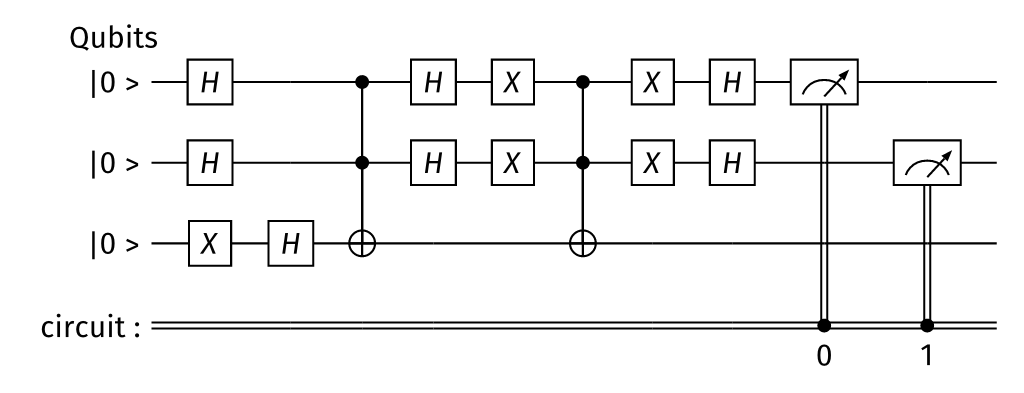
\includegraphics[width=0.9\textwidth]{images/basic-algorithms/3-qubits-grover.png}
    \caption{Grover-Algorithmus für $n=2$ (das gesuchte Element - $11$)}
    \label{fig:grover-three-bits}
\end{figure}

Zu Beginn, noch vor dem Start der Iterationen, müssen alle Qubits – einschließlich des Hilfsqubits – in eine Superposition gebracht werden. Dabei sollen sich zu Anfang alle Qubits im Zustand $0$ befinden, mit Ausnahme des Hilfsqubits, der vor der Hadamard-Operation in den Zustand $1$ gesetzt wird.\\

Nach Anwendung des Hadamard-Gatters befindet sich das Hilfsqubit somit im Zustand $\frac{1}{\sqrt{2}}(|0\rangle - |1\rangle)$, während alle übrigen Qubits den Zustand $\frac{1}{\sqrt{2}}(|0\rangle + |1\rangle)$ annehmen.

Anschließend beginnen die Iterationen. Jede Iteration besteht aus zwei Phasen. Die erste Phase ist die Anwendung der Orakelfunktion. Wie es in Grover-Algorithmus \ref{alg:grover} vorgestellt wurde, handelt es sich um eine Funktion, die effizient bestimmen kann, welcher Index dem gesuchten Element entspricht. Zwar kann diese Funktion den Index nicht direkt mitteilen, jedoch ist sie in der Lage, diesen Zustand mit einem Minuszeichen zu markieren.

Um das Funktionsprinzip des Algorithmus in diesem Beispiel besser zu verstehen, definieren wir eine vereinfachte Orakelfunktion manuell. Dabei ist zu beachten, dass die tatsächliche Orakelfunktion in der Praxis spezifisch an die jeweilige Aufgabe angepasst ist und daher möglicherweise anders implementiert wird. Auf die konkrete technische Realisierung der Orakelfunktion zur Datensuche gehen wir hier nicht ein, da dies den grundlegenden Ablauf von Grovers Algorithmus nicht beeinflusst.

Für das Verständnis des Grover-Algorithmus ist es entscheidend nachzuvollziehen, wie sich die Zustände der Qubits verändern, bis zum Zeitpunkt der Messung, die schließlich den gesuchten Index liefert.In diesem Beispiel haben wir als das gesuchte Index $11$ definiert - so wie es in dem Beispiel von Karten gab. Das bedeutet, dass die Messung am Ende genau dieses Ergebnis liefern soll. Wir modellieren daher ein Orakel, das genau diesen Index markiert. Als solche Orakelfunktion eignet sich das Toffoli-Gatter ($CCNOT$), das bei Ansteuerung beider Kontrollqubits mit dem Wert $1$ ein $X$-Gatter auf das Zielqubit – in diesem Fall das Hilfsqubit – anwendet:

\begin{definition}[Toffoli-Gatter]
\label{def:toffoli}
Das Toffoli-Gatter, auch bekannt als $CCNOT$-Gatter (für „controlled-controlled-not“), ist eine Erweiterung des bekannten $CNOT$-Gatters mit zwei Steuerbits und einem Zielbit. Das bedeutet: Das Zielbit (das dritte Bit) wird genau dann invertiert, wenn sowohl das erste als auch das zweite Steuerbit den Wert $1$ haben.(\cite{toffoli_proceedings_1980})
\end{definition}

Das Toffoli-Gatter sieht folgendermaßen aus:
\begin{figure}[H]
    \centering
    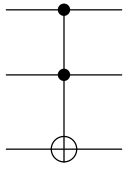
\includegraphics[width=0.2\textwidth]{images/basic-algorithms/toffoli.png}
    \caption{$CCNOT$ - Toffoli-Gatter}
    \label{fig:toffoli-gate}
\end{figure}

 Für die Zustände der oberen Qubits, die die Indizes $00$, $01$ und $10$ codieren, bleibt das Toffoli-Gatter ohne Wirkung – der Hilfsqubit verbleibt in dem Zustand $\frac{1}{\sqrt{2}}(|0\rangle - |1\rangle)$.\\

 Erst beim Index $11$ wird das Gatter aktiv: Es wendet das $X$-Gatter auf den Hilfsqubit an, wodurch dieser den Zustand $\frac{1}{\sqrt{2}}(|1\rangle - |0\rangle)$ annimmt \ref{def:toffoli}. Dieser lässt sich äquivalent als $-\frac{1}{\sqrt{2}}(|0\rangle - |1\rangle)$ schreiben – das Minuszeichen erscheint also vor dem gesamten Zustand.\\

 Dieses Minuszeichen bezieht sich nicht nur auf den Hilfsqubit, sondern auf den gesamten Zustand, der dem Index $11$ entspricht. Daher kann man den Hilfsqubit als unverändert betrachten und das Vorzeichen dem Zustand der oberen Qubits zuordnen. Damit ist der Index $11$ als der gesuchte Zustand mit einem Minus gekennzeichnet. Anders ausgedrückt: Die Orakelfunktion transformiert den Zustand $|11\rangle\,|q_{\text{3}}\rangle$ in $-|11\rangle\,|q_{\text{3}}\rangle$, wobei $|q_{\text{3}}\rangle$ den Zustand des Hilfsqubits bezeichnet.

Den Zustand des Quantensystems nach Anwendung des Orakels können wir folgendermaßen ausdrücken (der Hilfsqubit steht in der rechten Klammer):

$$
|\psi\rangle = \frac{1}{2\sqrt{2}} (|00\rangle + |01\rangle + |10\rangle - |11\rangle)(|0\rangle - |1\rangle)
$$

Damit ist der erste Teil der ersten Iteration abgeschlossen. Der gesuchte Index wurde markiert, aber eine sofortige Messung der Qubits würde keinen Nutzen bringen – das Minuszeichen zeigt sich im Messergebnis nicht. Außerdem würde der Index $11$ mit einer Wahrscheinlichkeit von nur $0{,}25$ erscheinen – genau wie alle anderen Indizes.

Um die weiteren Schritte besser zu verstehen, stellen wir uns die erste Hälfte des Algorithmus grafisch als Zustandsvektor vor. Die horizontale Achse definieren wir als Einheitsvektor, der alle Zustände der Superposition enthält – mit Ausnahme des gesuchten Zustands. Die vertikale Achse steht für den gesuchten Basiszustand.

Der Zustandsvektor $c$, also der Zustand des Systems vor der ersten Iteration, ist eine Linearkombination dieser beiden Basisvektoren entlang der horizontalen und vertikalen Achse.\ref{fig:initial-grover-three-qubits}

\begin{figure}[H]
    \centering
    \begin{tikzpicture}[scale=2]
    % Draw coordinate axes
    \draw[->] (-1.2, 0) -- (1.2, 0); % x-axis
    \draw[->] (0, -1.2) -- (0, 1.2); % y-axis

    % Draw the unit circle
    \draw (0,0) circle(1);

    % Angle theta
    \draw[->, thick] (0,0) -- (0.866,0.5); % hypotenuse (c)
    \node at (0.95,0.35) {$c$};

    % Projection on x-axis (a)
    \draw[->, thick] (0,0) -- (1,0);
    \node at (0.45,-0.08) {$a$};

    % Projection on y-axis (b)
    \draw[->, thick] (0,0) -- (0,1);
    \node at (-0.1,0.75) {$b$};

    % Angle label θ
    \draw (0.25,0) arc[start angle=0,end angle=30,radius=0.25];
    \node at (0.3,0.05) {$\theta$};
\end{tikzpicture}
    \caption{Der initiale Zustand des Systems}
    \label{fig:initial-grover-three-qubits}
\end{figure}

Im Fall dieses Beispiels (ein System aus zwei Qubits mit dem gesuchten Index $11$) lässt sich der Zustandsvektor $c$ durch die Koordinaten $x$ und $y$ wie folgt darstellen:

$$
\frac{1}{2}(|00\rangle + |01\rangle + |10\rangle + |11\rangle) = x \cdot \frac{1}{\sqrt{3}}(|00\rangle + |01\rangle + |10\rangle) + y \cdot |11\rangle
$$

\noindent Aus dieser Gleichung ergibt sich: $x = \frac{\sqrt{3}}{2}$ und $y = \frac{1}{2}$.\\

Anhand dieser Koordinaten erkennt man, dass der Winkel $\theta$ zwischen dem Vektor $c$ und der horizontalen Achse gleich $\frac{\pi}{6}$ ist. Vorausblickend lässt sich sagen: Unser Ziel ist es, diesen Winkel auf $\frac{\pi}{2}$ (oder zumindest in dessen Nähe) zu bringen – also den Zustand nahezu vollständig in Richtung des gesuchten Basiszustands zu drehen, sodass bei der anschließenden Messung mit hoher Wahrscheinlichkeit das gewünschte Ergebnis erscheint.

Die Koordinaten des aktuellen Zustandsvektors lassen sich über den Winkel $\theta$ wie folgt beschreiben:

$$
x = \cos{\theta}
$$
$$
y = \sin{\theta}
$$

Zur Klarstellung: Der Hilfsqubit wird in der Kreisdarstellung nicht berücksichtigt, da er nicht zur Codierung des Index dient, sondern lediglich zur Markierung des gesuchten Zustands verwendet wird.

Nach Anwendung der Orakelfunktion spiegelt sich der Zustandsvektor an der horizontalen Achse. Dies liegt daran, dass seine vertikale Komponente (der Anteil des Vektors $|11\rangle$) negativ wird. Der resultierende Vektor $c_{1b}$ ist somit die Spiegelung des ursprünglichen Vektors $c$ um den Winkel $\theta$ nach unten relativ zur Horizontalen:

\begin{figure}[H]
    \centering
\begin{tikzpicture}[scale=2.5]

    % Draw coordinate axes
    \draw[->] (-1.2, 0) -- (1.2, 0); % x-axis
    \draw[->] (0, -1.2) -- (0, 1.2); % y-axis

    % Draw the unit circle
    \draw (0,0) circle(1);

    % Main vector c (black)
    \draw[->, thick] (0,0) -- (0.866,0.5);
    \node at (0.95,0.35) {$c$};

    % Projection on x-axis (a)
    \draw[->, thick] (0,0) -- (1,0);
    \node at (0.45,-0.08) {$a$};

    % Projection on y-axis (b)
    \draw[->, thick] (0,0) -- (0,1);
    \node at (-0.1,0.75) {$b$};

    % First angle theta
    \draw (0.25,0) arc[start angle=0,end angle=30,radius=0.25];
    \node at (0.3,0.05) {$\theta$};

    % Second angle theta (for red vector)
    \draw[gray, ->] (0.2,0) arc[start angle=0,end angle=-30,radius=0.2];
    \node at (0.3,-0.08) {$\theta$};

    % Red vector c_{1b}
    \draw[->, thick, red] (0,0) -- (0.866,-0.5);
    \node[red] at (1.0,-0.4) {$c_{1b}$};

\end{tikzpicture}
    \caption{Der Zustand des Systems nach der ersten Teil der erste Iteration}
    \label{fig:after-first-part-grover-three-qubits}
\end{figure}

Diese Spiegelung erfolgt in diesem Beispiel durch die Anwendung des $CCNOT$-Gatters. Allgemein jedoch lässt sich dieser Schritt der Orakelfunktion durch folgende Operation beschreiben:

$$
U_{1b} = I - 2|b\rangle \langle b|
$$

Hier steht $U_{1b}$ für die Orakelfunktion. Diese Operation kehrt ausschließlich das Vorzeichen der vertikalen Komponente des Zustandsvektors um, was genau zur beschriebenen Spiegelung führt.

Überprüfen wir nun die Wirkung dieser Formel anhand des Beispiels:

\begin{align*}
U_{1b} |c\rangle &= (I - 2|11\rangle \langle 11|) \cdot \frac{1}{2}(|00\rangle + |01\rangle + |10\rangle + |11\rangle) \\
&= \frac{1}{2} \left( |00\rangle + |01\rangle + |10\rangle + |11\rangle - 2|11\rangle \right) \\
&= \frac{1}{2} (|00\rangle + |01\rangle + |10\rangle - |11\rangle)
\end{align*}

Damit ist der erste Teil der Iteration abgeschlossen.

Nun wenden wir uns dem zweiten Teil der ersten Iteration zu. In diesem Schritt erfolgt eine weitere Spiegelung – jedoch nicht mehr an der horizontalen Achse, sondern am ursprünglichen Zustandsvektor $c$. Es lässt sich leicht erkennen, dass der neue Zustandsvektor danach dem Ausdruck

$$
\cos(3\theta)|a\rangle + \sin(3\theta)|b\rangle
$$

\noindent entspricht. Das bedeutet, der Winkel zwischen dem Vektor und der horizontalen Achse ist nun $3\theta$. Der Zustand wurde also weiter in Richtung des gesuchten Basiszustands $|b\rangle$ gedreht.

\begin{figure}[H]
    \centering
\begin{tikzpicture}[scale=2]

    % Draw coordinate axes
    \draw[->] (-1.2, 0) -- (1.2, 0); % x-axis
    \draw[->] (0, -1.2) -- (0, 1.2); % y-axis

    % Draw the unit circle
    \draw (0,0) circle(1);

    % Main vector c (black)
    \draw[->, thick] (0,0) -- (0.866,0.5);
    \node at (0.95,0.35) {$c$};

    % Projection on x-axis (a)
    \draw[->, thick] (0,0) -- (1,0);
    \node at (0.45,-0.08) {$a$};

    % Projection on y-axis (b)
    \draw[->, thick] (0,0) -- (0,1);
    \node at (-0.1,0.75) {$b$};

    % First angle theta
    \draw (0.25,0) arc[start angle=0,end angle=30,radius=0.25];
    \node at (0.3,0.1) {$\theta$};

    % Second angle theta (for red vector)
    \draw[gray, ->] (0.2,0) arc[start angle=0,end angle=-30,radius=0.2];
    \node at (0.3,-0.08) {$\theta$};

    % Third angle theta (for red vector)
    \draw[gray, ->] (0.2,0.15) arc[start angle=30,end angle=60,radius=0.2];
    \node at (0.3,0.3) {$2\theta$};

    \draw[gray, ->] (0.6,-0.35) arc[start angle=0,end angle=35,radius=1.55];

    % Red vector c_{1b}
    \draw[->, thick, red] (0,0) -- (0.866,-0.5);
    \node[red] at (1.0,-0.4) {$c_{1b}$};

    % Green vector c_{1c}
    \draw[->, thick, green] (0,0) -- (0.5,0.866);
    \node[green] at (0.5,0.6) {$c_{1c}$};

\end{tikzpicture}
    \caption{Der Zustand des Systems nach der zweiten Teil der erste Iteration}
    \label{fig:after-second-part-grover-three-qubits}
\end{figure}
Die Operation zur Erzeugung des reflektierten Vektors $c_{1c}$ sieht wie folgt aus:

$$
U_{1c} = 2|c\rangle \langle c| - I
$$

Berechnen wir den resultierenden Vektor $c_{1c}$ für unser Beispiel:

\begin{align*}
U_{1c} |c_{1b}\rangle &= \left(2|c\rangle \langle c| - I\right) \cdot \frac{1}{2} (|00\rangle + |01\rangle + |10\rangle - |11\rangle) \\
&= |11\rangle
\end{align*}

Es fand eine Spiegelung des Zustandsvektors $|c_{1b}\rangle$ an $|c\rangle$ statt. Wenn man den Vektor $|c_{1b}\rangle$ als Linearkombination $k_1 |c\rangle + k_2 |c_{\perp}\rangle$ schreiben kann, wobei $|c_{\perp}\rangle$ senkrecht auf $|c\rangle$ steht und $k_1$, $k_2$ reelle Koeffizienten sind, dann ergibt sich der gespiegelte Vektor zu:

$$
k_1 |c\rangle - k_2 |c_{\perp}\rangle
$$

Genau dies geschieht hier: Die Komponente entlang $|c\rangle$ bleibt erhalten, während die senkrechte Komponente ihr Vorzeichen ändert. In unserer Quantenschaltung wird dieser zweite Teil der Iteration folgendermaßen implementiert:

\begin{figure}[h!]
    \centering
    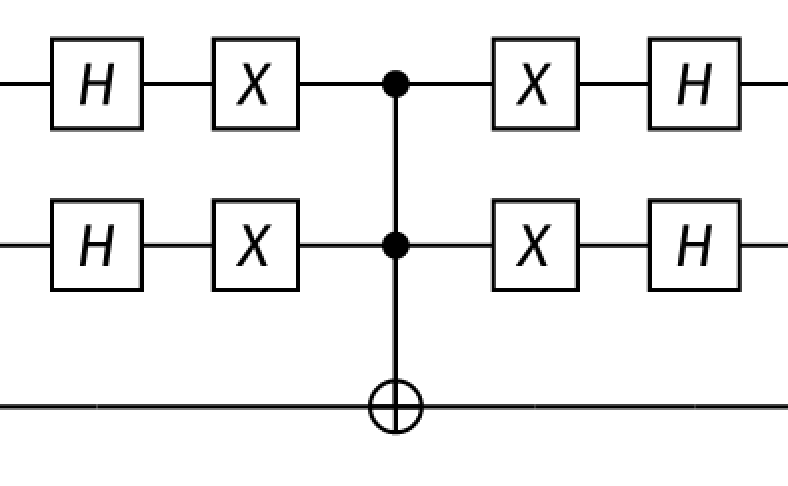
\includegraphics[width=0.4\textwidth]{images/basic-algorithms/grover-2-iteration.png}
    \caption{Zweite Iteration - $U_{1c}$}
    \label{fig:grover-second-iteration}
\end{figure}

Zunächst wird der Hadamard-Operator auf den ersten und zweiten Qubit angewendet. Dies vereinfacht unsere Aufgabe erheblich, da die Reflexion des Zustandsvektors nun nicht mehr relativ zum Superpositionszustand $\frac{1}{2}(|00\rangle + |01\rangle + |10\rangle + |11\rangle)$ erfolgen muss, sondern relativ zum Zustand $|00\rangle$.

Um die Spiegelung durchzuführen, müssten wir eigentlich allen Zuständen außer dem Nullzustand ein negatives Vorzeichen zuweisen. Stattdessen nutzen wir jedoch einen Trick: Wir versehen lediglich den Zustand $|00\rangle$ mit einem Minuszeichen und lassen alle übrigen Superpositionszustände unverändert. Dies erreichen wir durch eine gezielte Abfolge von Gattern: zuerst $X$-Gatter, dann ein $CCNOT$-Gatter, und danach wird die Transformation durch Umkehr der Schritte rückgängig gemacht – also erneut $X$-Gatter und anschließend Hadamard-Gatter.

Aufgrund dieses Tricks (Negation nur des Nullzustands) ergibt sich in unserem Beispiel mit zwei Qubits nicht $|11\rangle$, sondern $-|11\rangle$ als Ergebnis – abgesehen von einer globalen Phase. Dies ist jedoch unproblematisch, da sich die globale Phase beim Messen nicht auswirkt und wir den gesuchten Index trotzdem korrekt erhalten.

Aus der Darstellung auf dem Einheitskreis, die den Zustand des Systems nach der zweiten Hälfte der ersten Iteration veranschaulicht, wird deutlich, dass der Zustandsvektor mit jeder weiteren Iteration der Vertikalen näherkommt. In unserem konkreten Fall beträgt der Winkel zwischen Zustandsvektor und Horizontaler nach Abschluss der ersten Iteration bereits $3\theta$, was genau dem gewünschten Winkel $\frac{\pi}{2}$ entspricht.

Im allgemeinen Fall ergibt sich der Winkel nach $t$ Iterationen zu:

$$
(2t + 1)\theta \approx \frac{\pi}{2}
$$

Daraus lässt sich die erforderliche Anzahl an Iterationen für den Grover-Algorithmus bestimmen. Wenn $t$ groß ist und $K = 1$ (für $K > 1$ ist der Schluss analog), wird der Winkel $\theta$ sehr klein. Daher kann man $\theta$ durch $\sin{\theta}$ ersetzen, und es gilt näherungsweise:

$$
\theta \approx \sin{\theta} = \frac{1}{\sqrt{N}}
$$

Daraus folgt:

$$
(2t + 1) \cdot \frac{1}{\sqrt{N}} \approx \frac{\pi}{2}
$$

Wenn man die Eins im Term $(2t + 1)$ vernachlässigt (für große $t$ zulässig), erhält man:

$$
t \approx \frac{\pi \sqrt{N}}{4}
$$

Wie wir bereits gesehen haben, besteht jede Iteration aus zwei Schritten. Der erste Schritt ist die Reflexion nach unten an der Horizontalen. Der zweite Schritt ist die Reflexion nach oben an der ursprünglichen Richtung, also am Vektor $c$. Dabei wird der Zustandsvektor stets auf einen größeren Winkel nach oben reflektiert als der Winkel der vorherigen Spiegelung nach unten. Genau dadurch nähert sich der Vektor bei jeder Iteration schrittweise der Vertikalen.\\

Wir haben ein Beispiel für die Anwendung des Grover-Algorithmus betrachtet. Im nächsten Kapitel werden wir uns mit der Zeitkomplexität beschäftigen und erläutern, warum dieser Algorithmus trotz der Anzahl an Iterationen dennoch schneller ist als klassische Suchalgorithmen.


\subsection{Komplexitätsanalyse}
Der Grover‐Algorithmus durchsucht eine unstrukturierte Datenbank der Größe \(N\) mithilfe eines Quantenorakels in \(\Theta(N)\) Orakelaufrufen. Anders ausgedrückt: Während die klassische Vollsuche im Mittel \(\Theta(N)\) Prüfungen erfordert, reduziert Grover die Zahl der notwendigen Prüfungen auf etwa $\frac{\pi}{4}\,\sqrt{N}\ $ das heißt auf die Quadratwurzel der Datenbankgröße.

Aus Sicht der Komplexitätstheorie bezeichnet man die Eingangsgröße mit \(n\), so dass $N = 2^n$.
Die Laufzeit des Grover‐Algorithmus lässt sich daher durch  
$O\bigl(2^{n/2}\bigr)$ beschreiben. Obwohl dies gegenüber dem klassischen \(O(2^n)\) einen erheblichen quadratischen Gewinn darstellt, wächst der Algorithmus bei zunehmender Zahl der Suchbits weiterhin exponentiell.

Die untere Schranke aus der Arbeit von Bennett–Bernstein–Brassard–Vazirani (\cite{zotero-1212}) zeigt, dass kein Quantenalgorithmus im Black‐Box‐Modell mit weniger als  
\[
\Omega(\sqrt{N})
\]  
Orakelaufrufen auskommen kann.(\cite{zotero-1211}) Damit ist der Grover‐Algorithmus in diesem Modell asymptotisch optimal: Ohne zusätzliche Struktur in der Datenbank lässt sich kein suprakquadratischer (etwa exponentieller) Vorteil erzielen.  


\section{Klassifikation von Algorithmen nach Zeitkomplexität}

Im Rahmen der theoretischen Informatik werden Entscheidungsprobleme nach der zur Lösung benötigten Zeit in verschiedene Klassen eingeordnet. Dabei interessiert insbesondere, welche Probleme auf einem klassischen bzw. quantenmechanischen Modell in polynomieller Zeit lösbar sind, und wie sich diese Klassen zueinander verhalten.\\

Zunächst versteht man unter der Klasse \(\mathbf{P}\) jene Probleme, für die es deterministische Algorithmen gibt, die auf einem klassischen Computer in polynomieller Zeit laufen. Formal heißt das: Ein Problem liegt in \(\mathbf{P}\), wenn es einen Algorithmus gibt, dessen Laufzeit durch einen Polynomausdruck \(O(n^k)\) für eine feste Konstante \(k\) beschränkt ist, wobei \(n\) die Eingabegröße bezeichnet. Probleme aus \(\mathbf{P}\) gelten als praktisch effizient lösbar, sofern der Exponent \(k\) nicht zu groß wird.\\

Die Klasse \(\mathbf{NP}\) (nondeterministic polynomial time) umfasst diejenigen Entscheidungsprobleme, bei denen eine etwaige Lösung auf einem klassischen Computer in polynomieller Zeit verifizierbar ist, auch wenn ein deterministischer polynomieller Lösungsalgorithmus bislang unbekannt ist. Ein typisches Beispiel ist das Teilmengen-Summen-Problem: Legt man dem Algorithmus als „Zertifikat“ eine vermutete Teilmenge vor, so kann man in \(O(n)\) bzw. \(O(n\log n)\) Zeit nachprüfen, ob die Summe den Zielwert ergibt.\\

Innerhalb von \(\mathbf{NP}\) existieren die \(\mathbf{NP}\)-\emph{vollständigen} Probleme (\(\mathbf{NP}\)\emph{-complete}), die zu den schwierigsten \(\mathbf{NP}\)-Problemen zählen. Ein Problem \(L\) ist genau dann \(\mathbf{NP}\)-vollständig, wenn \(L\in\mathbf{NP}\) und jedes andere Problem aus \(\mathbf{NP}\) in polynomieller Zeit auf \(L\) reduziert werden kann. Die berühmte \textsc{Clique}-Frage oder das \textsc{3-SAT}-Problem sind klassische Vertreter dieser Klasse. Gelingt es, eines dieser Probleme in polynomieller Zeit zu lösen, so hätte man damit einen polynomiellen Algorithmus für alle \(\mathbf{NP}\)-Probleme.\\

Die Klasse der \(\mathbf{NP}\)-\emph{harten} Probleme (\(\mathbf{NP}\)\emph{-hard}) enthält solche Probleme, auf die sich beliebige \(\mathbf{NP}\)-Probleme in polynomieller Zeit reduzieren lassen. Im Gegensatz zu \(\mathbf{NP}\)-vollständigen Problemen müssen \(\mathbf{NP}\)-harte Probleme selbst nicht in \(\mathbf{NP}\) liegen und können etwa gar nicht entscheidbar sein oder nur in exponentieller Zeit verifizierbar sein.\\

Wenn man zusätzlich zur deterministischen Rechenmaschine Zufallsbits zulässt und die Wahrscheinlichkeit, die richtige Entscheidung zu treffen, für positive und negative Instanzen jeweils oberhalb eines festen Schwellwerts (typischerweise \(>1/2\)) liegt, definiert man die Klasse \(\mathbf{BPP}\) (bounded‑error probabilistic polynomial time). Probleme in \(\mathbf{BPP}\) lassen sich mit Monte‑Carlo‑Algorithmen in polynomieller Zeit mit beliebig kleiner Fehlerrate lösen.(\cite{zotero-1212}) \\

Der quantenmechanische Gegenpart zu \(\mathbf{BPP}\) ist die Klasse \(\mathbf{BQP}\) (bounded‑error quantum polynomial time).(\cite{zotero-1212}) Hierbei kann ein Quantenalgorithmus für ein Problem in polynomieller Zeit auf einem Quantencomputer mit hoher Wahrscheinlichkeit das korrekte Ergebnis liefern. Ein bekanntes Beispiel ist die Ganzzahlfaktorzerlegung großer Zahlen mittels Shor’s Algorithmus, der das hierfür klassische \(\mathbf{NP}\)-Problem in polynomieller Zeit auf einem Quantencomputer löst.

\begin{figure}[h]
  \centering
  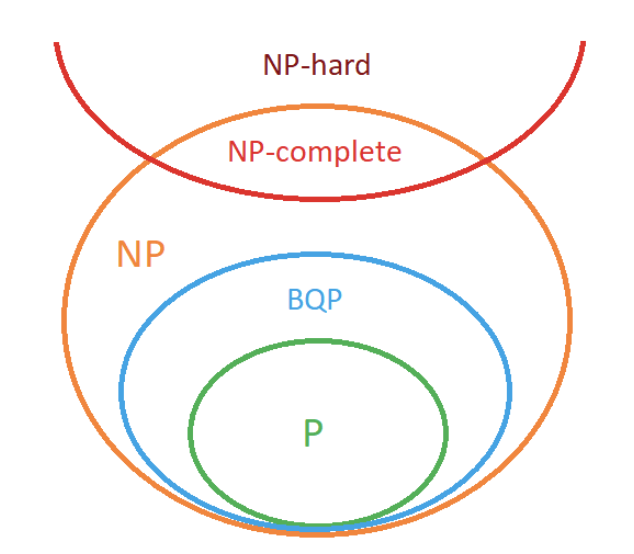
\includegraphics[width=0.7\textwidth]{images/basic-algorithms/problem-classes.png}
  \caption{Übersicht der wichtigsten Zeitkomplexitätsklassen: \(\mathbf{P}\subseteq \mathbf{BQP}\subseteq \mathbf{NP}\subseteq \mathbf{NP}\text{-hard}\) und die Lage von \(\mathbf{NP}\)-complete Problemen innerhalb von \(\mathbf{NP}\).}
  \label{fig:problem_classes}
\end{figure}

Abschließend lässt sich festhalten, dass die Frage, ob \(\mathbf{P}=\mathbf{NP}\) gilt, zu den bedeutendsten offenen Problemen der Informatik zählt. Auch der Vergleich zwischen klassischen und quantenmechanischen Modellen, speziell die Vermutung \(\mathbf{P}\subsetneq \mathbf{BQP}\subseteq \mathbf{NP}\), prägt die Forschung im Bereich effizienter Algorithmen maßgeblich.

\section{Quantum Safe Algorithmen}

\subsection*{Einleitung}

Mit der rasanten Entwicklung von Quantencomputern stehen klassische Verschlüsselungsverfahren vor einer existenziellen Bedrohung. Während heutige Systeme auf der Annahme beruhen, dass bestimmte mathematische Probleme schwer zu lösen sind, können Quantenalgorithmen wie \textit{Shor’s Algorithmus} oder \textit{Grover’s Algorithmus} diese Probleme effizient berechnen – und damit die Sicherheit brechen, auf die heutige digitale Kommunikation angewiesen ist.

Diese Bedrohung macht sogenannte \textbf{Quantum Safe Algorithmen} notwendig – kryptographische Verfahren, die auch gegen Angriffe durch leistungsfähige Quantencomputer resistent sind. Zwei Hauptansätze stehen im Zentrum der Forschung:

\begin{itemize}
  \item \textbf{Quantum Key Distribution (QKD)} – ein Verfahren, das physikalische Gesetze der Quantenmechanik nutzt, um absolut sichere Schlüsselverteilungen zu ermöglichen.
  \item \textbf{Post-Quantum Cryptography (PQC)} – klassische, quantenresistente Algorithmen, die auf heutigen Geräten ausgeführt werden können.
\end{itemize}

In diesem Kapitel werfen wir einen Blick auf beide Ansätze – und erläutern insbesondere die jüngsten Fortschritte durch das NIST (National Institute of Standards and Technology), das 2022 erste standardisierungsreife Algorithmen bekannt gegeben hat.

\subsection{Quantum Key Distribution}

Quantum Key Distribution (QKD) ermöglicht es, kryptografische Schlüssel über unsichere Kanäle zu übertragen – mit einem entscheidenden Vorteil: Jeder Abhörversuch verändert unweigerlich den Zustand der übertragenen Quanteninformation und kann somit erkannt werden.

Ein klassisches Beispiel für ein QKD-Protokoll ist das \textbf{BB84-Protokoll}, das 1984 von Bennett und Brassard entwickelt wurde und später, im Jahr 2000, von Peter W. Shor and John Preskill geprüft wurde. Es nutzt die Polarisation von Photonen, um binäre Informationen zu codieren. Der Ablauf besteht aus drei Phasen:

\begin{itemize}
  \item \textbf{Key Exchange:} Alice sendet zufällig polarisierte Photonen an Bob, der sie in zufällig gewählten Basen misst.
  \item \textbf{Key Sifting:} Über einen klassischen Kanal gleichen beide ihre verwendeten Basen ab und behalten nur die Werte, bei denen die Basen übereinstimmten.
  \item \textbf{Key Distillation:} Durch Stichproben wird geprüft, ob Abhörversuche stattfanden. Die finale Schlüssellänge ergibt sich nach dieser Bereinigung.
\end{itemize}

\noindent Neben BB84 existieren weitere bedeutende Protokolle:

\begin{itemize}
  \item \textbf{B92} (reduzierte Variante mit zwei Zuständen)
  \item \textbf{E91} (nutzte erstmals Quantenverschränkung)
  \item \textbf{BBM92}, \textbf{SARG04}, \textbf{DPS}, \textbf{COW}, \textbf{GG02} (verschiedene Weiterentwicklungen)
\end{itemize}

Für eine detaillierte Übersicht der Protokolle und deren Unterschiede siehe das Paper:
\textit{An Overview of Quantum-Safe Approaches: Quantum Key Distribution and Post-Quantum Cryptography} von Guobin Xu et al.

\subsection{Post-Quantum Cryptographie Algorithmen}

Da QKD mit hohen technischen und infrastrukturellen Anforderungen verbunden ist, setzt sich in der Praxis vor allem die \textbf{Post-Quantum Cryptography (PQC)} durch. Sie nutzt klassische Rechenverfahren, basiert jedoch auf mathematischen Problemen, die auch für Quantencomputer als schwierig gelten.

Das US-amerikanische \textbf{NIST} hat im Rahmen eines mehrjährigen Wettbewerbs Verfahren für zwei Hauptkategorien gesucht:

\begin{itemize}
  \item \textbf{Public-Key Encryption and Key Establishment (KEM)}
  \item \textbf{Digitale Signaturverfahren}
\end{itemize}

\noindent Nach mehreren Runden wählte NIST im Juli 2022 vier Algorithmen aus, die als erste Quantum Safe Standards empfohlen werden.

\noindent Für Verschlüsselung und Schlüsselaustausch nominierte NIST:

\begin{itemize}
  \item \textbf{CRYSTALS-Kyber} – 2017, J. Bos et al.
\end{itemize}

\vspace{0.5em} % optionaler vertikaler Abstand

\noindent Für digitale Signaturen nominierte NIST:

\begin{itemize}
  \item \textbf{CRYSTALS-Dilithium} – 2018, L. Ducas et al.

  \item \textbf{Falcon} – 2018, P.-A. Fouque et al.

  \item \textbf{SPHINCS+} – 2019, D. J. Bernstein et al.
\end{itemize}

\subsubsection*{CRYSTALS-Kyber}

\textbf{CRYSTALS-Kyber} ist ein \textit{lattice-basiertes Key Encapsulation Mechanism (KEM)}. Es basiert auf dem sogenannten \textit{Module Learning with Errors (MLWE)}-Problem, das auch von Quantencomputern bislang nicht effizient gelöst werden kann.

Der Algorithmus nutzt Polynomarithmetik und besteht aus drei Hauptschritten:

\begin{enumerate}
  \item \textbf{Schlüsselerzeugung:} Öffentlicher und privater Schlüssel werden erzeugt.
  \item \textbf{Encapsulation:} Ein gemeinsamer Schlüssel wird erzeugt und verschlüsselt übertragen.
  \item \textbf{Decapsulation:} Der Empfänger entschlüsselt den Schlüssel mit seinem privaten Schlüssel.
\end{enumerate}

\noindent Kyber bietet drei Sicherheitsniveaus, die sich durch unterschiedliche Parametergrößen unterscheiden und an klassische AES-Sicherheitsstufen angelehnt sind:

\begin{itemize}
  \item \textbf{Kyber-512} – Sicherheitsniveau 1 (vergleichbar mit AES-128)
  \item \textbf{Kyber-768} – Sicherheitsniveau 3 (vergleichbar mit AES-192)
  \item \textbf{Kyber-1024} – Sicherheitsniveau 5 (vergleichbar mit AES-256)
\end{itemize}

\subsubsection*{CRYSTALS-Dilithium}

\textbf{CRYSTALS-Dilithium} ist ein digitaler Signaturalgorithmus, ebenfalls basierend auf \textit{MLWE} und \textit{MSIS} (Module Short Integer Solution). Die Signaturerzeugung verwendet die \textit{Fiat-Shamir-Transformation}, die aus einem interaktiven Zero-Knowledge-Protokoll eine nicht-interaktive Signatur macht.

Dilithium bietet drei Sicherheitsniveaus:

\begin{itemize}
  \item \textbf{Dilithium2}
  \item \textbf{Dilithium3}
  \item \textbf{Dilithium5}
\end{itemize}

Die Vorteile liegen in der schnellen Verifikation, der Robustheit gegen Seitenkanalangriffe und der guten Performance. Diese Eigenschaften machen Dilithium zu einem führenden Kandidaten im Bereich der quantensicheren digitalen Signaturen.
\printbibliography
%\motto{Use the template \emph{chapter.tex} to style the various elements of your chapter content.}
\chapter{Fehlerkorrektur}
\label{error_correction} % Always give a unique label
% use \chaptermark{}
% to alter or adjust the chapter heading in the running head

\chapterauthor{Niklas Bodfeld, Tim Boschert, Manuel Meixner, Ann-Kathrin Wenzel}

\abstract{some abstract}

\section{Fehlertypen in Quantenrechnern}\label{chap:QEC1}

\subsection{Die Herausforderung von Fehlern in Quantencomputern}
Die praktische Realisierung der Quantencomputer steht vor einer grundlegenden Hürde. Die Fehler. Diese treten in Quantensystemen häufiger auf als in klassischen Rechnern. Zudem sind sie viel schwerer zu kontrollieren.

Während klassische Systeme mit extrem niedrigen Fehlerraten arbeiten (unter 10⁻¹⁷), liegen diese bei heutigen Quantenprozessoren um Größenordnungen zwischen 10⁻³ und 10⁻¹. Der Grund dafür liegt unteranderem in der hohen Empfindlichkeit von Qubits gegenüber Umwelteinflüssen wie elektromagnetischen Feldern, Temperaturfluktuationen oder Strahlungen. Hinzu kommen Fehler durch ungenaue Hardware, Crosstalk zwischen benachbarten Qubits und unzuverlässige Mess- oder Initialisierungsprozessen.\ref{chap:QEC3}.). \cite[Seite 48-49]{tutschku_quantencomputing_2023}; \ref{chap:QEC3}.)

Die Auswirkungen dieser Fehler sind tiefgreifend. Schon ein einzelner Fehler kann sich durch Verschränkung auf das gesamte System ausbreiten. Besonders kritisch sind Phasenfehler, da sie die Interferenzmuster zerstören können, auf denen viele Quantenalgorithmen beruhen.

Deshalb ist die Entwicklung effektiver Fehlerkorrekturmethoden ein zentrales Thema für die Zukunft des Quantencomputings. Nur wenn bestimmte Mechanismen greifen, kann der theoretische Nutzen in der Praxis ausgeschöpft werden.


\subsection{Physikalische Fehlerursachen in Quantenrechnern}
Quantencomputer arbeiten nicht mit Bits sondern mit Qubits, die sich gleichzeitig in mehreren Zuständen befinden können. Die quantenmechanischen Eigenschaften von Qubits, insbesondere die Superposition, ermöglichen das enorme Potenzial und die Leistungsstärke von Quantencomputern. Gleichzeitig machen sie Quantencomputer allerdings auch extrem empfindlich. Schon geringe äußere Einflüsse können die Zustände stören und zu Fehlern führen. Im Folgenden werden zentrale physikalische Ursachen näher betrachtet.


\textbf{Dekohärenz}

Da sich physikalische Qubits nicht vollständig von ihrer Umgebung isolieren lassen, kommt es durch unvermeidliche Wechselwirkungen zu Dekohärenz, einem zentralen Fehlermechanismus in der Quanteninformatik.
Dekohärenz beschreibt den Prozess, bei dem ein Qubit durch den Kontakt mit seiner Umgebung „gestört“ wird und dabei seine Fähigkeit verliert, sich in einem Überlagerungszustand zu befinden. Stattdessen verhält es sich zunehmend wie ein klassisches Bit. Das bedeutet, dass die Quanteninformation, die zuvor im Zustand des Qubits gespeichert war, verloren geht. Anders als klassische Fehler entsteht Dekohärenz nicht durch eine fehlerhafte Bedienung oder ungenaue Operationen, sondern ist ein grundlegendes physikalisches Phänomen, das automatisch auftritt, sobald ein Quantensystem mit seiner Umgebung interagiert.

Es wird dabei zwischen Phasendekohärenz und Amplitudendekohärenz unterschieden. Bei der Phasendekohärenz bleibt das Qubit formal im selben Zustand, also zum Beispiel in ∣0⟩ oder ∣1⟩, jedoch verändert sich die relative Phase zwischen diesen Zuständen. Diese Phase ist zentral für Quanteninterferenz, einem Grundprinzip, das es Quantencomputern ermöglicht, durch Überlagerung unterschiedliche Rechenwege effizient zu nutzen. Wird die Phase gestört, kann der Quantencomputer falsche oder keine sinnvollen Ergebnisse mehr liefern. 

Amplitudendekohärenz hingegen beschreibt einen echten Energieverlust des Qubits. Wenn es aus einem angeregten Zustand ∣1⟩ in den Grundzustand ∣0⟩ zurückfällt. Solche Prozesse treten unter anderem durch spontane Emission oder Wärmeaustausch mit der Umgebung auf und sind in physischen Systemen wie supraleitenden Qubits oder Ionenfallen besonders häufig zu beobachten.

Die Wirkung solcher Umweltkopplungen lässt sich mathematisch mithilfe der sogenannten Operator-Summen-Zerlegung (Kraus-Zerlegung) beschreiben. Die Zerlegung erlaubt es, die Störung eines Qubits durch die Umgebung als Wahrscheinlichkeitsmischung mehrerer Fehlerprozesse darzustellen. Dies ist entscheidend für die Entwicklung von Quantenfehlerkorrektur und bildet die theoretische Grundlage für den Umgang mit Umwelteinflüssen.

Ein häufig verwendetes Modell zur Beschreibung solcher Fehler ist das lokale und Markov’sche Fehlermodell. Es geht davon aus, dass jedes Qubit nur mit seiner eigenen lokalen Umgebung interagiert (lokal) und dass sich diese Umgebung bei jedem Zeitschritt erneuert bzw. unabhängig vom Zustand in vorherigen Zeitintervallen ist (Markov). Die Gesamtwirkung auf ein Mehr-Qubit-System lässt sich dann als Produkt von Einzeleffekten auf die jeweiligen Qubits darstellen. Dieses Modell ist realistisch und erlaubt es, die meisten heute verwendeten Quantenfehlerkorrekturverfahren zu formulieren. 

Insgesamt zeigt sich, dass Dekohärenz  ein unvermeidlicher, aber mathematisch gut beschreibbarer Effekt ist. Durch geeignete Fehlerkorrektur und die Annahme realistischer Fehlermodelle kann ihre Auswirkung auf Quanteninformationen deutlich reduziert werden. \ref{chap:QEC3}.). \cite[Seite 332-339]{rieffel_eleanor_g_and_wolfgang_h_polak_quantum_2011}


\textbf{Rauschen und Vibration}

Doch Dekohärenz ist nicht die einzige physikalische Fehlerursache in Quantencomputern. Weitere Ursachen liegen in verschiedenen Rauschprozessen. Das sind zufällige oder unkontrollierte Störungen aus der Umgebung. Dazu zählen unter anderem thermisches Rauschen, das durch Temperaturunterschiede entsteht, sowie elektromagnetische Fluktuationen, verursacht durch Stromleitungen, elektronische Geräte oder sogar Mobilfunkstrahlung. Auch mechanische Vibrationen stellen eine Störquelle dar. Diese können beispielsweise durch Pumpen oder Bewegungen im Kühlapparat ausgelöst werden und sich auf die empfindlichen Qubits übertragen. In Systemen wie Ionenfallen können solche Vibrationen die Bewegung der Ionen stören. Dies führt dazu, dass die Quantenobjekte ihre Überlagerungszustände verlieren und sich zunehmend klassisch verhalten. Gleichzeitig wirken zufällige elektrische Feldschwankungen auf die Teilchen, wodurch es zu unkontrollierten Energie- und Positionsänderungen kommen kann. Wird dabei das harmonische Potenzial gestört, verlassen die Ionen ihren quantenmechanischen Grundzustand, was zu Rechenfehlern führt. Besonders problematisch wird dies bei stark gekoppelten Qubits, bei denen viele Operationen wie CNOT-Gatter notwendig sind. Denn jede zusätzliche Operation erhöht die Anfälligkeit für Rauschen und überfordert in vielen Fällen die heutigen Fehlermitigationstechniken. Um diese Fehler zu minimieren, sind hochstabile Betriebsbedingungen sowie gezielte Kühl- und Isolationsmaßnahmen unerlässlich.\ref{chap:QEC3}.). \cite[Seite 39-43]{tutschku_quantencomputing_2023}; \ref{chap:QEC3}.). \cite[Seite 353-356]{nielsen_michael_a_and_isaac_l_chuang_quantum_2010}


\textbf{Unvollständige Isolation}

Ein besonderes Problem ist die unzureichende Isolation der Qubits. Idealerweise sollte ein Qubit vollständig von seiner Umgebung abgeschottet sein. In der Realität ist das fast nicht möglich. Selbst im Vakuum oder bei extrem tiefen Temperaturen gibt es noch mikroskopisch kleine Wechselwirkungen mit anderen Teilchen, Materialien oder Defekten. Manche Materialien enthalten zum Beispiel sogenannte Zwei-Niveau-Systeme, die mit den Qubits interagieren können und als zusätzliche Störquellen wirken. Auch kosmische Strahlung oder Magnetfelder aus der Umgebung können Störungen verursachen (Tutschku et al., 2023).

Aus all diesen Gründen ist es extrem wichtig, die Quantenhardware so gut wie möglich gegen äußere Einflüsse zu schützen. Das geschieht zum Beispiel durch ultratiefe Temperaturen im Millikelvin-Bereich, durch spezielle Abschirmungen gegen elektromagnetische Wellen, durch mechanische Entkopplung der Geräte und durch den Einsatz besonders reiner Materialien ohne Defekte. Trotzdem lässt sich nie ganz vermeiden, dass äußere Einflüsse auf das System wirken. Daher ist es bedeutend, zusätzlich auf softwareseitige Verfahren zur Fehlerkorrektur zu setzen.\ref{chap:QEC3}.). \cite[Seite 24-26]{tutschku_quantencomputing_2023}

Quantenfehler sind ein Zusammenspiel aus unvermeidbaren physikalischen Prozessen, technologischen Grenzen und Umwelteinflüssen. Sie zu verstehen und zu kontrollieren ist eine der größten Herausforderungen beim Bau und Betrieb eines funktionierenden Quantencomputers.

\subsection{Klassifizierung von Quantenfehlern}\label{chap:QEC1.3}
Die Klassifikation von Quantenfehlern stellt eine bedeutsame Grundlage für die Entwicklung stabiler Fehlerkorrekturverfahren im Quantencomputing dar. Aufgrund der Superposition können Fehler nicht nur den Zustand selbst, sondern auch die relative Phase, Amplitude oder die Kohärenzeigenschaften eines Qubits beeinflussen. Die Einteilung unterscheidet zwischen diskreten, kontinuierlichen, zufälligen und systematischen Fehlern.

Die Diskrete Fehlerarten sind die Pauli-Fehler. Die einfachste und zugleich mathematisch fundamentale Klasse von Quantenfehlern basiert auf den sogenannten Pauli-Fehlern, benannt nach den drei Pauli-Matrizen 
X, Y und Z. Diese Operatoren stellen Basisoperationen im zweidimensionalen Qubit-Zustandsraum dar und bilden eine vollständige Fehlerbasis für beliebige Ein-Qubit-Störungen.


\textbf{Bit-Flip-Fehler (X-Fehler)}

Ein Bit-Flip-Fehler ist eine der einfachsten und grundlegendsten Fehlerarten in der Quanteninformatik. Er beschreibt eine Umkehrung des Zustands eines Qubits, also einen Wechsel von ∣0⟩ nach ∣1⟩ oder von ∣1⟩ nach ∣0⟩. Formal wird dieser Fehler durch den X-Operator (auch Pauli-X-Gatter genannt) dargestellt, der wie ein klassisches NOT-Gatter wirkt: X∣0⟩=∣1⟩, X∣1⟩=∣0⟩. Ein solcher Fehler kann in der physikalischen Realität zum Beispiel durch thermische Anregung entstehen. Also wenn ein Qubit spontan aus dem Grundzustand ∣0⟩ in einen angeregten Zustand ∣1⟩ übergeht, weil es mit seiner Umgebung Energie austauscht.

Beim Bit-Flip-Fehler geht es also ausschließlich um die Veränderung der Besetzungszustände eines Qubits, nicht um seine Phase oder Superposition. Er ist die quantenmechanische Entsprechung eines klassischen Bitfehlers, bei dem eine „0“ zu einer „1“ wird oder umgekehrt. \ref{chap:QEC3}.). \cite[Seite 246-251]{rieffel_eleanor_g_and_wolfgang_h_polak_quantum_2011}(Nielsen & Chuang, 2010, S.449).



\textbf{Phase-Flip-Fehler (Z-Fehler)}

Ein Phase-Flip-Fehler (auch Z-Fehler) ist eine fundamentale Art von Fehler in der Quanteninformationstheorie, die nicht den Zustand ∣0⟩ oder ∣1⟩ selbst verändert, sondern die relative Phase zwischen ihnen. Formal wird dieser Fehler durch den Z-Operator (Pauli-Z-Gatter) dargestellt: Z∣0⟩=∣0⟩,Z∣1⟩=−∣1⟩. Obwohl sich der Zustand ∣1⟩ dabei nicht in ∣0⟩ umwandelt, bekommt er ein negatives Vorzeichen. Die sogenannte Phaseninversion. Für Zustände wie ∣0⟩ oder ∣1⟩ alleine ist dieser Effekt nicht direkt sichtbar. Doch sobald der Qubit-Zustand eine Superposition ist, wirkt sich der Fehler messbar aus. Besonders deutlich wird das in diesem Zustand: \[
|+\rangle = \frac{1}{\sqrt{2}}(|0\rangle + |1\rangle)
\]
Wird darauf der Z-Operator angewendet, entsteht:
\[
Z|+\rangle = \frac{1}{\sqrt{2}}(|0\rangle - |1\rangle) = |-\rangle
\]

Damit wird die Phase zwischen den beiden Zustandsanteilen vertauscht. Das hat gravierende Folgen für Quantenalgorithmen, die auf Interferenz und kohärenter Phasenevolution beruhen. Phase-Flip-Fehler stören also genau diese empfindlichen quantenmechanischen Effekte, die Quantencomputer leistungsfähig machen. \ref{chap:QEC3}.). \cite[Seite 251-252]{rieffel_eleanor_g_and_wolfgang_h_polak_quantum_2011}


\textbf{Kombinierte Bit- und Phase-Fehler (Y-Fehler)}

Der Y-Operator kombiniert Bit- und Phase-Flip in einem einzigen Fehler: Y=iXZ. Er wirkt gleichzeitig wie ein X- (Bit-Flip) und ein Z-Operator (Phase-Flip), und ist damit der vollständigste Einzelfehler im Pauli-Basisset. Solche Fehler treten typischerweise bei komplexeren physikalischen Störungen auf. Dazu zählt unteranderem Crosstalk zwischen benachbarten Qubits, Störfelder mit nichtlokaler Auswirkung oder gekoppelte Fluktuationen in Steuerleitungen. In der Fehlerkorrektur werden Y-Fehler daher als gleichzeitiges Auftreten von X- und Z-Fehlern behandelt und können entsprechend über Stabiliser-Messungen erkannt werden (Rieffel & Polak, 2011, S.375).

Diese drei Operatoren bilden eine vollständige Fehlerbasis für Ein-Qubit-Störungen. Jeder beliebige Fehler auf einem Qubit kann mathematisch als Linearkombination von I, X, Y und Z dargestellt werden. Diese Eigenschaft ist von Bedeutung für den Aufbau von Quantenfehlerkorrekturcodes wie dem Shor-Code oder dem Steane-Code, welche gezielt auf Pauli-Fehler reagieren. \ref{chap:QEC3}.). \cite[Seite 252-253]{rieffel_eleanor_g_and_wolfgang_h_polak_quantum_2011}


\textbf{Dämpfung}

Neben diskreten Fehlern gibt es die kontinuierliche Fehlerprozesse, die sich über sogenannte Quantenkanäle modelliert werden. Die zwei wichtigsten Beispiele sind Amplitudendämpfung und die Phasendämpfung. Sie hängen eng mit den physikalischen Prozessen der Phasen- und Amplitudendämpfung zusammen.

Die Amplitudendämpfung beschreibt den Verlust von Energie durch das Qubit, etwa infolge spontaner Emission oder thermischer Relaxation. Der Zustand ∣1⟩ relaxiert dabei mit einer gewissen Wahrscheinlichkeit γ in den Grundzustand ∣0⟩.
 \ref{chap:QEC3}.). \cite[Seite 380-383]{nielsen_michael_a_and_isaac_l_chuang_quantum_2010}
(Nielsen & Chuang, 2010, S.376–377)

Bei der Phasendämpfung (Dephasing) geht keine Energie verloren, aber Kohärenz. Die Off-Diagonal-Elemente der Dichtematrix, also die, die Superpositionen erzeugen, werden gedämpft. Dies geschieht durch Umwelteinflüsse wie Fluktuationen elektromagnetischer Felder. In der Praxis ist Phasendämpfung oft die dominante Dekohärenzquelle. \ref{chap:QEC3}.). \cite[Seite 383-386]{nielsen_michael_a_and_isaac_l_chuang_quantum_2010}(Rieffel & Polak, 2011, S.374–375).


\textbf{Zufällige vs. Systematische Fehler}

Quantenfehler lassen sich nicht nur nach ihrer physikalischen Form, sondern auch nach ihrer Entstehungsart klassifizieren. Hierzu zählen zufällige Fehler und systematische Fehler.

Zufällige Fehler (stochastisch) entstehen unvorhersehbar durch thermisches Rauschen, Photonen-Einfälle, kosmische Strahlung oder spontane Kopplungen an die Umgebung. Sie sind oft kurzzeitig, unkorreliert und lassen sich statistisch modellieren.
Systematische Fehler beruhen auf wiederholbaren, deterministischen Einflüssen, wie falscher Kalibrierung von Pulssequenzen, ungenauen Gatterzeiten oder falsch modellierter Kopplung. Solche Fehler summieren sich über Zeit auf und können ganze Rechenprozesse verfälschen. Sie sind schwerer zu korrigieren, da sie nicht durch Mittelwertbildung „herausrauschen“.\ref{chap:QEC3}.). \cite[Seite 3-5]{Quantum error correction below the surface code threshold_2024}
Die Unterscheidung ist für die Architekturplanung bedeutend, da systematische Fehler oft durch verbesserte Hardware, kontrollierte Steuerungen oder modellgestützte Korrektur vermieden werden können.

Ein wachsendes Problem in größeren Quantenprozessoren ist das Auftreten von korrelierten Fehlern. Solche Fehler beeinflussen mehrere Qubits gleichzeitig und können durch gemeinsame Störquellen oder durch ungewollte Kopplungen entstehen. Anders als unabhängige Fehler breiten sie sich nicht lokal aus, sondern erzeugen komplexe Fehlerbilder, die von klassischen Fehlerkorrekturmodellen oft nicht erfasst werden.


\subsection{Hardwarebedingte Fehler und Systematische Grenzen}
Neben den oben beschriebenen Fehlern spielen auch hardwarebedingte Fehler eine zentrale Rolle in der Fehlertheorie des Quantencomputings. Diese entstehen durch Unzulänglichkeiten in der technischen Umsetzung der Steuerung, der Auslese und der physikalischen Qubit-Architektur. In realen Quantenprozessoren, wie supraleitenden Schaltkreisen, Ionenfallen oder spinbasierten Systemen, sind diese Fehlerquellen ein wesentlicher begrenzender Faktor für die Skalierbarkeit und Zuverlässigkeit der Systeme.


\textbf{Gatteroperationen}

Ein wesentliches Problem sind fehlerhafte Gatteroperationen. Idealerweise sollen Quantenlogikgatter wie das CNOT- oder Hadamard-Gate eine definierte unitäre Transformation auf den Zustand der Qubits ausführen. In der Praxis weichen die implementierten Operationen von diesem Ideal ab. Ursachen dafür sind unter anderem folgende Fehler:

Timing-Fehler: Ungenauigkeiten in der Pulslänge oder -frequenz führen zu nicht vollständig abgeschlossenen Rotationen.
Crosstalk: Eine ungewollte Kopplung zwischen benachbarten Qubits oder Steuerleitungen kann zu Störungen führen, die nicht auf das Zielqubit beschränkt bleiben.
Leakage-Fehler: Besonders bei supraleitenden oder mehrstufigen Systemen kann ein Qubit durch ein Gatter in höhere Energiezustände außerhalb des Rechenraums (z.B. |2⟩) übergehen, was spätere Gates unbrauchbar macht.
Falsche Kalibrierung: Abweichungen in der Kalibrierung der Steuerpulse führen dazu, dass Operationen (z.B. ein X-Gate) nicht exakt das tun, was vorgesehen ist – etwa eine Rotation um 178° statt 180°.

Diese Gatterfehler häufen sich über tiefe Schaltkreise hinweg und führen dazu, dass die logische Fehlerrate mit zunehmender Schaltungstiefe exponentiell ansteigt. Selbst bei modernen Quantenprozessoren liegt die mittlere Gatterfidelität, also die Wahrscheinlichkeit, mit der ein Gatter korrekt ausgeführt wird, typischerweise nur bei 99–99,9%. \ref{chap:QEC3}.). \cite[Seite 2-5]{Quantum error correction below the surface code threshold_2024}; \ref{chap:QEC3}.). \cite[Seite 5-13]{Time–adaptive single–shot crosstalk detector on superconducting quantum computer_2025}


\textbf{Messfehler}

Ein weiterer kritischer Aspekt sind Messfehler. Die Auslese eines Qubits erfolgt in der Regel über die Verstärkung und Analyse eines quantenmechanischen Signals. Dabei können verschiedene Fehlerquellen auftreten. Zum Beispiel elektronisches Rauschen in der Verstärkerschaltung, Überlappung der Signalverteilungen für die Zustände ∣0⟩ und ∣1⟩ oder Verzögerungen und Sättigungseffekte in der Ausleseelektronik. Solche Störungen können dazu führen, dass der tatsächliche Zustand des Qubits falsch interpretiert wird. Dies beeinträchtigt nicht nur die Genauigkeit von Quantenalgorithmen, sondern besonders auch die Fehlerkorrektur, die auf das zuverlässige Auslesen von Syndromen angewiesen ist.
 \ref{chap:QEC3}.). \cite[Seite 49-51]{tutschku_quantencomputing_2023}; \cite[Seite 5-7]{Time–adaptive single–shot crosstalk detector on superconducting quantum computer_2025}


\textbf{Qubitinitalisierung}

Die Initialisierung von Qubits ist ein grundlegender Schritt zu Beginn jeder Quantenberechnung. Ziel ist es, sämtliche Qubits zuverlässig in den Grundzustand ∣0⟩ zu bringen. In der Praxis gelingt dies jedoch nicht immer mit perfekter Genauigkeit. Mögliche Ursachen sind zum Beispiel thermische Anregungen bei unzureichender Kühlung, unvollständige Relaxation aus angeregten Zuständen oder Restkopplungen an Resonatoren oder benachbarte Qubits. Fehlerhafte Initialisierungen beeinflussen unmittelbar die Ausführung der ersten Gatteroperationen und können sich über den gesamten Quantenschaltkreis hinweg auswirken. \ref{chap:QEC3}.). \cite[Seite 3-5]{Quantum error correction below the surface code threshold_2024}


\textbf{Konnektivität}

In skalierbaren Architekturen, vor allem in zweidimensionalen Gittern supraleitender Qubits, sind nicht alle Qubits direkt miteinander verbunden. Diese eingeschränkte Konnektivität führt dazu, dass logische Operationen, die Qubits an weit entfernten Positionen betreffen, durch zusätzliche SWAP-Gatter oder Relaisoperationen realisiert werden müssen. Diese zusätzlichen Schritte erhöhen nicht nur die Rechenzeit, sondern fügen dem System zusätzliche Fehlerquellen hinzu. Besonders kritisch ist dies in tiefen Schaltkreisen oder bei komplexen Algorithmen. \ref{chap:QEC3}.). \cite[Seite 49-51]{tutschku_quantencomputing_2023}


\textbf{Kalibrierfehler}

Alle oben genannten Fehlerarten werden zusätzlich durch Kalibrierfehler verstärkt. Diese entstehen, wenn die physikalischen Parameter des Systems, wie Frequenzen, Kopplungsstärken, Pulsamplituden oder Dämpfungsraten nicht exakt bekannt oder nicht stabil sind. Selbst kleine Abweichungen in der Kalibrierung können über viele Rechenzyklen hinweg zu signifikanten Abweichungen im Endergebnis führen. Studien zeigen, dass Kalibrierfehler insbesondere bei nicht regelmäßig durchgeführten Rekalibrierungszyklen zu systematischer Fehlentwicklung der Qubit-Zustände führen. \ref{chap:QEC3}.). \cite[Seite 5-7]{Quantum error correction below the surface code threshold_2024}

\subsection{Quantifizierung und Modellierung von Quantenfehlern}
Die präzise Modellierung und Quantifizierung von Fehlern in Quantencomputern ist wichtig, um deren Auswirkungen auf die Informationsverarbeitung zu verstehen und wirksame Fehlerkorrekturstrategien zu entwickeln. Aufgrund der Besonderheiten quantenmechanischer Systeme, insbesondere Superposition, Nichtklassikalität und Unitarität, ist eine Beschreibung von Fehlerprozessen nur durch formalisierte mathematische Modelle möglich, die über klassische Störmodelle weit hinausgehen. In der Theorie offener Quantensysteme werden solche Fehler durch Quantenkanäle beschrieben, deren Wirkung über sogenannte Krausoperatoren modelliert wird.


\textbf{Fehlerkanäle und Krausoperatoren}

Ein Quantenkanal beschreibt die Wirkung eines Umgebungseinflusses auf ein Quantensystem, das sich dadurch in einen neuen Zustand überführt. Formal wird ein Quantenkanal (E) durch eine completely positive, trace-preserving (CPTP) Abbildung auf dem Raum der Dichtematrizen definiert. Die Wirkung eines solchen Kanals auf einen Zustand ρ wird durch die Kraus-Zerlegung beschrieben:

E(\rho) = \sum_k E_k \rho E_k^\dagger, \quad \text{mit} \quad \sum_k E_k^\dagger E_k = I.

Hierbei sind  E_k die Krausoperatoren, die jeweils eine mögliche Fehlerwirkung modellieren. Diese Darstellung ist besonders mächtig, da sie sowohl diskrete als auch kontinuierliche Fehlermechanismen integriert. Je nach Art des Rauschprozesses ergeben sich unterschiedliche konkrete Kanalformen:
Amplitudendämpfungskanal: Modelliert Energieverluste wie spontane Emission. Dabei relaxiert das Qubit mit Wahrscheinlichkeit 
γ vom angeregten Zustand ∣1⟩ in den Grundzustand ∣0⟩. Die zugehörigen Krausoperatoren lauten:

E_0 = \begin{pmatrix} 1 & 0 \\ 0 & \sqrt{1-\gamma} \end{pmatrix},E_1 = \begin{pmatrix} 0 & 0 \\ \sqrt{\gamma} & 0 \end{pmatrix}


Depolarisationskanal: Beschreibt symmetrisches Rauschen, bei dem mit Wahrscheinlichkeit p ein zufälliger Pauli-Fehler (X, Y, Z) auftritt:

E(\rho) = (1-p)\rho + \frac{p}{3}(X\rho X + Y\rho Y + Z\rho Z)


Diese Modelle bilden die Grundlage für theoretische Fehleranalysen und sind integraler Bestandteil moderner Simulationen von Quantenalgorithmen.\ref{chap:QEC3}.). \cite[Seite 379-397]{nielsen_michael_a_and_isaac_l_chuang_quantum_2010}


\textbf{Fehlerraten}

Fehlerraten spielen eine zentrale Rolle bei der Quantifizierung und Modellierung von Quantenfehlern, insbesondere im Kontext der derzeit verfügbaren NISQ-Quantencomputer („Noisy Intermediate-Scale Quantum“). Diese Systeme sind durch verschiedene Störfaktoren stark limitiert. Dazu zählen kurze Kohärenzzeiten (T1 und T2), begrenzte Qubit-Konnektivität, Crosstalk und insbesondere die Fehlerraten bei Quantengattern und Messungen. Die Gate-Fidelity, also die Wahrscheinlichkeit, mit der ein Quantengatter korrekt ausgeführt wird, liegt derzeit bei etwa 0,1% Fehler für 1-Qubit-Gatter und etwa 1% Fehler für 2-Qubit-Gatter. Auch bei der Initialisierung und Auslesung treten mit etwa 1% signifikante Fehler auf. Diese Fehlerraten sind um Größenordnungen höher als bei klassischen Computern und schränken die maximale Schaltungstiefe sowie die Verlässlichkeit von Quantenalgorithmen massiv ein. Um diese Fehler systematisch zu erfassen und vergleichbar zu machen, wurden Metriken wie das „Quantenvolumen“ entwickelt. Es kombiniert Aspekte wie Qubit-Anzahl, Gate-Fidelity und Schaltungstiefe zu einer einzigen Kenngröße. Allerdings ist diese Metrik nicht unumstritten, da die Aussagekraft stark vom konkreten Anwendungsfall abhängt. In jedem Fall ist eine präzise Quantifizierung und Modellierung der Fehlerraten unerlässlich, um die Einsatzfähigkeit von Quantencomputern realistisch bewerten zu können und eine effektive Fehlerkorrektur zu ermöglichen. \ref{chap:QEC3}.). \cite[Seite 379-397]{https://www.quantencomputer-info.de/quantencomputer/welche-quantencomputer-gibt-es-jetzt-schon/}


\textbf{Fehlergrenzen und Fehlertolernaz}

Ein zentrales Konzept in der Quantenfehlertoleranz ist die sogenannte Fehlergrenze (Threshold). Diese beschreibt den maximal tolerierbaren physikalischen Fehler \( p \) der Qubits, unterhalb dessen ein Fehlerkorrekturcode in der Lage ist, die logische Fehlerwahrscheinlichkeit 
\( p_{L} \) 
durch Vergrößerung des Codes zu unterdrücken. Ist der physikalische Fehler kleiner als der Schwellenwert \( p_{L} \) , kann die logische Fehlerquote beliebig klein gemacht werden. Der Code wirkt also stabilisierend. Liegt der physikalische Fehler jedoch über diesem Schwellenwert, wird die Fehlerkorrektur kontraproduktiv und verschlechtert den Zustand. Für den in der Praxis besonders relevanten Surface Code liegt der theoretische Schwellenwert bei etwa 10,9•% (bei separater Behandlung von X- und Z-Fehlern). Mit realistischen Decodierungsalgorithmen liegt der praktische Schwellenwert bei etwa 10,3•%.

Ein weiterer kritischer Aspekt ist die Fehlertoleranz (Fault Tolerance) von Quantenfehlerkorrekturverfahren. Dabei geht es nicht nur darum, Fehler im Qubit-Zustand selbst zu erkennen und zu beheben, sondern auch Fehler, die während des Korrekturprozesses auftreten, beispielsweise bei Zwei-Qubit-Gates oder bei der Syndrommessung, korrekt zu behandeln. Eine fehlertolerante Fehlerkorrektur muss gewährleisten, dass sich solche Fehler nicht unkontrolliert ausbreiten. Dies wird beispielsweise durch spezielle Schaltungen, redundante Hilfsqubits (Ancillas) oder wiederholte Messungen über mehrere Zyklen erreicht. Diese zusätzlichen Anforderungen erhöhen jedoch den Ressourcenbedarf erheblich. In realistischen Szenarien, insbesondere bei Surface Codes mit fehlerhaften Syndrommessungen, reduziert sich der Schwellenwert dadurch auf etwa 1 %. Dennoch ist dieser Wert für moderne Quantenhardware erreichbar, da aktuelle Systeme bereits Fehlerquoten unterhalb dieser Grenze aufweisen.\ref{chap:QEC3}.). \cite[Seite 13-15]{roffe_Quantum_error_correction_2019} 

\subsection{Auswirkungen von Fehlern auf Quantenalgorithmen und Systemarchitektur}
Fehler haben tiefgreifende Auswirkungen auf die Funktionsweise von Quantenalgorithmen und die Gestaltung von Quantencomputer-Architekturen. Bereits kleinste Abweichungen durch Umwelteinflüsse oder ungenaue Operationen können den empfindlichen Quantenzustand stören. Solche Störungen zeichnen sich in Form von Dekohärenz, Gate-Fehlern und Messfehlern ab. Besonders kritisch ist die Dekohärenz, also der Verlust von Quantenkohärenz, die essenziell für Superpositions- und Verschränkungszustände ist. Algorithmen wie Shor’s oder Grover’s, die stark auf Interferenzeffekten beruhen, werden dadurch extrem fehleranfällig. Ein einzelner Fehler kann das gesamte Interferenzmuster zerstören und damit das korrekte Ergebnis verhindern. \ref{chap:QEC3}.). \cite[Seite 381-385]{nielsen_michael_a_and_isaac_l_chuang_quantum_2010} 

Diese hohe Fehleranfälligkeit wirkt sich direkt auf die algorithmische Struktur aus. Je größer die Schaltungstiefe, also die Anzahl nacheinander geschalteter Operationen, desto wahrscheinlicher treten Fehler auf. Aktuelle Hardware beschränkt die maximale Tiefe daher erheblich. Entwickler müssen daher bereits beim Entwurf von Quantenalgorithmen Strategien zur Fehlertoleranz berücksichtigen. Ein zentrales Konzept in diesem Zusammenhang ist der sogenannte Fehlerschwellenwert (Threshold), der angibt, bis zu welchem Maß an physikalischen Fehlern eine zuverlässige Fehlerkorrektur überhaupt möglich ist \ref{chap:QEC3}.). \cite[Seite 293-308]{rieffel_eleanor_g_and_wolfgang_h_polak_quantum_2011}.

Auch auf der Systemarchitektur wirkt sich die Fehleranfälligkeit massiv aus. Um fehlerhafte physikalische Qubits nutzbar zu machen, werden sie in logische Qubits zusammengefasst, die durch Fehlerkorrekturcodes geschützt sind, wie durch den Steane- oder Shor-Code . Dieser Schritt ist jedoch teuer. Die Anzahl der tatsächlich benötigten physikalischen Qubits steigt exponentiell mit dem Anspruch an Fehlertoleranz. Beispielsweise kann ein logisches Qubit je nach Code und Fehlerrate mehrere Hundert oder Tausend physikalische Qubits benötigen \ref{chap:QEC3}.). \cite[Seite 435–437]{nielsen_michael_a_and_isaac_l_chuang_quantum_2010};\ref{chap:QEC3}.). \cite[Seite 246-253]{rieffel_eleanor_g_and_wolfgang_h_polak_quantum_2011}.

Liegt die effektive Fehlerrate pro Gatteroperation oder Qubit unterhalb dieser Fehlerschwelle, so kann durch wiederholte Korrekturzyklen ein logisch fehlerfreier Zustand aufrechterhalten werden. Wird sie überschritten, kann auch ein noch so ausgeklügelter Fehlerkorrekturcode das System nicht mehr retten.

Die Gestaltung der Quantenhardware und -architektur muss daher darauf ausgerichtet sein, mit einer begrenzten Anzahl physikalischer Qubits möglichst effektive Fehlerresistenz zu gewährleisten. Dazu gehören unteanderm Fehlertolerante Layouts, z.B. zweidimensionale Qubit-Gitter mit lokaler Nachbarschaftsstruktur, die einfache Syndrome-Messung und Korrektur ermöglichen.
Die konkrete Umsetzung solcher Codes, wie etwa des 9-Qubit Shor-Codes, zeigt, dass verschiedene Arten von Fehlern, wie der Bit-Flip, Phase-Flip und kombinierte Fehler, durch geeignete Verschränkung und Syndrommessung identifiziert und korrigiert werden können. Dies setzt jedoch eine Systemarchitektur voraus, die gezielte Paarung und Interaktion zwischen Qubits erlaubt, was hohe Anforderungen an die Qubit-Konnektivität und Kohärenz stellt.

Fehler wirken sich aber nicht nur auf die Hardware, sondern auch auf die Softwareebene aus. Quantenalgorithmen müssen so entworfen sein, dass sie entweder robust gegenüber Fehlern sind oder mit reduzierten Ressourcen für Fehlerkorrektur arbeiten. Dafür werden auch softwarebasierte Fehlermitigationstechniken verwendet, etwa die statistische Nachbearbeitung von Messergebnissen oder hybride Strategien, bei denen klassische Optimierung zur Steuerung kurzer Quantenzyklen genutzt wird \ref{chap:QEC3}.). \cite[Seite 305-306]{rieffel_eleanor_g_and_wolfgang_h_polak_quantum_2011}.

Zusammenfassend lässt sich sagen, dass die Fehleranfälligkeit in Quantencomputern kein nachträgliches Problem darstellt, sondern ein grundlegendes Designkriterium auf allen Ebenen. Von der Wahl der Algorithmen über die Anzahl und Anordnung der Qubits bis hin zur Steuerungselektronik. Nur wenn es gelingt, Fehler systematisch zu modellieren, zu korrigieren oder zu umgehen, können Quantencomputer ihr volles Potenzial entfalten.


\section{Grundprinzipien in Quantenfehlerkorrektur}\label{chap:QEC2}
\subsection{Fehlererkennung ohne Zustandsmessung}
Eines der zentralen Konzepte der Quanten-Fehlerkorrektur ist, dass man Fehler erkennen kann, ohne die kodierte Quanteninformation zu messen und somit zu zerstören. In klassischen Systemen könnten wir etwa redundante Bitmuster verwenden, um Fehler aufgrund direkter Messung zu erkennen und zu korrigieren. In einem quantenmechanischen System ist es jedoch nicht so einfach möglich, eine Messung durchzuführen, da ein solcher Schritt den Superpositionszustand des Qubits kollabieren ließe und damit die gespeicherte Information unter Umständen irreversibel zerstören könnte. \cite{nielsen_michael_a_and_isaac_l_chuang_quantum_2010}

Um das zu umgehen, führt man im Bereich der Quanten-Fehlerkorrektur sogenannte Syndrommessungen durch. Dabei handelt es sich um Messungen, bei denen nicht der Zustand des Qubits direkt gemessen wird, sondern nur Information über das Eintreten von Fehlern. Man misst dabei den sogenannten Stabilisator-Operator, der zu einem speziellen Quanten-Fehlerkorrekturcode gehört. Diese Operatoren definieren eine Menge erlaubter Zustände – sogenannte +1-Eigenzustände der Stabilizer-Gruppe. Tritt ein Fehler auf, so verändert sich die Eigenwertstruktur des Stabilisators. Ein Wechsel zwischen \(+1\) und \(-1\) ist zum Beispiel ein  Zeichen dafür, dass ein bestimmter Fehler passiert. \cite[Seite 444-446]{nielsen_michael_a_and_isaac_l_chuang_quantum_2010}

Die Syndrommessung erfolgt in der Praxis meist so, dass man Hilfsqubits (Ancillae) einführt, auf denen man den Stabilisator wirken lässt und so Informationen darüber erhält, was der Stabilizer auf den gekodeten Zustand angewendet hätte, ohne hierbei den gekodeten Zustand zu verändern. So lassen sich ernsthaft Fehler zum Beispiel durch die sogenannten kontrollierten Operatoren auch zu dem Hilfs-Qubit "weiterleiten" und damit dort auslesen. Dabei bleibt die gekodete Quanteninformation erhalten. Man nutzt dies dazu, das sogenannte Fehlersyndrom zu bestimmen um dann gezielt unitäre Korrektur-Operatoren durchzuführen (siehe Kapitel \ref{chap:QEC3}.). \cite[Seite 444-446]{nielsen_michael_a_and_isaac_l_chuang_quantum_2010}

Ein Schlüsselelement des fehlertoleranten Quantencomputings ist die Möglichkeit, einen Quantenzustand messen zu können, ohne dass er in seinen Ursprungszustand zu zwei Drittelwahrscheinlichkeit kollabiert. Dank dieser Fähigkeit können Codes konstruiert werden, welche die Integrität von Quanteninformation auch dann noch lange Zeit sicherstellen, wenn wiederkehrende Fehler laufend erkannt und ausgebessert werden.

\subsection{Redundanz durch Kodierung}
Quanten-Fehlerkorrektur beruht auf zentraler Idee, Quantenzustände vor Fehlern zu schützen, indem Redundanz eingefügt wird. Das bedeutet, ein einzelnes logisches Qubit wird nicht durch ein einziges physikalisches Qubit dargestellt, sondern auf mehrere physikalische Qubits verteilt. Genau durch diese zusätzliche Kodierungskapazität können Fehler eintreten, ohne dass dabei die logische Quanteninformation verloren geht.

Im Unterschied zur klassischen Fehlerkorrektur, bei der Redundanz verwendet wird (z.B. dreifache Paritätsbits), muss in der Quantenwelt solch ein Ansatz jedoch mit Bedacht gewählt werden. Denn das No-Cloning-Theorem verhindert, dass man auch einfach unbekannte Quantenzustände duplizieren kann. \cite{nielsen_michael_a_and_isaac_l_chuang_quantum_2010} Stattdessen wird die Kodierung mithilfe einer kohärenten Verschränkung mehrerer Qubits erreicht, sodass die Quanteninformation nicht in einem einzelnen Qubit, sondern in einem höherdimensionalen Unterraum des Gesamtsystems gespeichert wird.

Ein bekanntes Beispiel ist der Shor-Code, bei dem ein logisches Qubit auf neun physikalische Qubits abgebildet wird. Dieser Code schützt sowohl vor Bit-Flip- als auch vor Phase-Flip-Fehlern, indem er erst eine dreifache Kopie erstellt, um Bit-Flips zu entdecken, dann jede dieser Kopien nochmals mit einer Phase-Flip-Korrektur kodiert. \cite{shor_scheme_1995}
Ebenso gut ist der Steane-Code, der sieben Qubits zum Darstellen eines logischen Qubits verwendet und den klassischen (7, 4, 3)-Hamming-Code verwendet. \cite{Steane}

Mit Hilfe einer solchen Kodierung kann Quanteninformation in einem sogenannten Code-Raum abgelegt werden, der durch eine Gruppe von Stabilisator-Operatoren definiert ist. Tritt ein Fehler auf, so wird der Zustand in einen orthogonalen Unterraum verschoben, der außerhalb des Code-Raums liegt. Dieses Umschichten lässt sich über die Syndrommessung identifizieren – und zwar ohne, dass der ursprüngliche Zustand vermessen wird. Wesentlich ist, dass die Redundanz dabei hilft, Fehler zu lokalisieren und Korrekturoperationen durchzuführen, ohne die Quantenkohärenz zu stören.

Die Redundanz durch Kodierung ist somit die Voraussetzung für alle Quanten-Fehlerkorrekturverfahren: Denn nur indem man Information auf viele Qubits verteilt, kann man dem System Fehler \(\)verzeihen, ohne dass es aus funktionalem Zerfallen lässt.

\subsection{Fehlerzustände müssen unterscheidbar sein}
Ein entscheidendes Konzept in der Quantenfehlerkorrektur ist, dass Fehler auf einfache Weise voneinander unterscheidbar sein müssen. Nur wenn Fehler Zustände auf unterschiedliche Weise beschädigen, hat man eine Chance, festzustellen welcher der Fehler aufgetreten ist, mit dem Ziel diesen gezielt zu korrigieren ohne die Quanteninformation zu verlieren.

In der Sprache der Quanteninformatik bedeutet dies, dass die durch Fehler erstellten Zustände orthogonal zueinander sein müssen, beziehungsweise so aufgebaut, dass man durch Messung eines fehlerhaften Zustands auf den Code-Raum schließen kann. Andernfalls besteht die Gefahr, dass Fehler, die zu gleichem Messausgang führen, nicht unterschieden werden können und die Messung zu einer falschen Korrektur und dem Verlust von Information führt. \cite[Seite 449–451]{nielsen_michael_a_and_isaac_l_chuang_quantum_2010}

Dieses Konzept wird durch das sogenannte Fehlerkorrekturkriterium mathematisch präzisiert. Für eine Menge von Fehlern \(\left\{E_{i}\right\}\) , die von einem Quantencode korrigiert werden sollen, gilt:
\begin{equation}
    \left\langle\psi_{a}\right| E_{i}^{\dagger} E_{j}\left|\psi_{b}\right\rangle=C_{i j} \delta_{a b}
\end{equation}
für alle Zustände \(
    \left|\psi_{a}\right\rangle,\left|\psi_{b}\right\rangle
\)  im Code-Raum. Hierbei hängt die Konstante \(
    C_{i j}
\) vom Fehler,  nicht jedoch vom kodierten Zustand ab. Dieses Kriterium ist notwendig um sicherzustellen, dass die Wirkung eines Fehlers unabhängig von der gespeicherten Information eindeutig bestimmbar ist.

Aber aufgepasst: Wenn zwei unterschiedliche Fehler denselben Effekt auf den Code haben – also nicht unterscheidbar sind –, kann keine gezielte Korrektur erfolgen. Die Fähigkeit zur Unterscheidung solcher Fehlerzustände ist also die Voraussetzung für \textit{irgendeine} syndrombasierte Fehlerkorrektur. Nur dadurch können beispielsweise Look-Up-Tabellen oder automatische Fehlerkorrekturmechanismen sicher die \textit{einzig mögliche} Korrektur wählen.

Das Prinzip hat übrigens eine Parallele zur Konstruktion von Stabilizer-Codes, bei denen unterschiedliche Fehler unterschiedliche Syndrommuster hinterlassen. Durch geschickte Wahl der Stabilisatorgruppe kann man erreichen, dass in einem Stabilizer-Code alle Fehler innerhalb der Toleranzgrenze eindeutige Syndrome haben. \cite{gottesmann Stabilizer Codes}

\subsection{Reversibilität}
Ein entscheidendes Prinzip der Quanten-Fehlerkorrektur ist es, dass sämtliche eingesetzten Operationen im Fehlerkorrekturprozess umkehrbar sein müssen. In der Quantenmechanik entsprechen sämtliche möglichen zeitlichen Entwicklungen von isolierten Systemen unitären Transformationen – also Operationen, die völlig umkehrbar sind und keine Information vernichten. Diese Forderung gilt es auch für die Fehlerkorrektur durchzusetzen, da eine unwiderrufliche Fehlerkorrektur notwendigerweise den kodierten Quantenzustand zerstören und die Kohärenz der Quanteninformation verlieren würde. \cite[Seite 450-451]{nielsen_michael_a_and_isaac_l_chuang_quantum_2010}

Anders ausgedrückt: Wenn bei einer Kette von Ereignissen ein Fehler durch das Syndrom erkannt wurde, erfolgt ihre Korrektur durch eine bestimmte, unitäre Operation, welche uns den Fehlerzustand wieder ins Urteil des Codes zurückführt. Ist dieser Zustand erreicht, ist unser Fehler nicht nur korrigiert, sondern auch so, dass wir ihn\textbf{ kohärent rekonstruieren} können – und dies ist für weiteres Quantenrechnen und für fehlerresistente Quantenrechner notwendig.

Dieses Erfordernis der Rückkehr zur Ausgangslage besitzt auch eine sehr klare und bequeme theoretische Beschreibung: Das sogenannte Nicht-Trivialitätskriterium für Fehlerkorrektur sagt uns, dass für jede nichttriviale Fehlerwirkung \(E_i\) eine zugehörige Korrekturoperation \(R_i\) existiert, so dass 
\begin{equation}
    R_{i} E_{i}|\psi\rangle=|\psi\rangle \quad \text { für alle }|\psi\rangle \in \mathcal{C}
\end{equation}
Die Fehlererkennung und -korrektur insgesamt bildet somit einen Prozess, bei dem der Quanteninformationsträger lediglich entlang eines Umwegs durch Code-Hilfsraum entlanggeführt wird und die Logikqubit-Effektivität erhalten bleibt, um in der Lage zu sein, auch weitere Quantengatter auf diese anzuwenden.

Darum unterscheidet sich die Quanten-Fehlerkorrektur deutlich z.B. von klassischen Korrekturverfahren, welche nicht unbedingt reversibel sein müssen. In der Quanteninformatik wiederum ist Reversibilität jedoch ein \textbf{fundamentales physikalisches Prinzip}, das sowohl theoretisch als auch bei der Praxis der Implementierung beachtet werden muss.

\subsection{Fehlerlokalisierung}
Ein weiteres wichtiges Konzept, das hinter der Quanten-Fehlerkorrektur steckt, ist das der Fehlerlokalisierung. Damit ist gemeint, dass ein aufgetretener Fehler am besten so gefunden und behandelt werden kann, dass er sowohl räumlich als auch logisch eng eingegrenzt ist, und dass seine Folgen sich nicht unkontrolliert über das gesamte System ausbreiten. Nur wenn ein Fehler örtlich identifiziert und korrigiert werden kann, ist eine skalierbare und robuste Fehlerkorrektur möglich. \cite[Seite 451-452]{nielsen_michael_a_and_isaac_l_chuang_quantum_2010}

Fehler können in einem Quantencomputer verschiedene Ursprünge haben – z. B. Dekohärenz, Wechselwirkung mit der Umwelt oder Fehler bei Gates. Nach dem Prinzip der Fehlerlokalisierung sollte jeder dieser Fehler anfänglich lediglich eine begrenzte Anzahl physikalischer Qubits beeinflussen. Diese Voraussetzung soll es ermöglichen, mittels sogenannter Syndrommessungen zu erkennen, wo ein Fehler aufgetreten ist, ohne dabei den globalen Quantenzustand zu zerstören.

Dieses Konzept ist eng mit der Verwendung sogenannter lokaler Fehlerkorrektur-Codes wie z. B. topologischen Codes wie dem Surface Code verbunden. Bei diesen Codes sind die Qubits in einer regelmäßigen, zweidimensionalen Gitteranordnung angeordnet, bei der jeder Stabilizer-Operator nur Qubits betrachtet, die benachbart sind. Ein auftretender Fehler produziert ein lokales Syndrom, das sich aus den Nachbarn des fehlerhaften Qubits ergibt. Dadurch kann der Fehler nicht nur gefunden, sondern auch eingegrenzt und so gezielt korrigiert werden. \cite{Fowler et al}

Insbesondere für große, skalierbare Quantenrechner ist die Fähigkeit zur Fehlerlokalisierung essentiell: Denn ohne diese müssten sämtliche Qubits miteinander verschränkt und abgefragt werden, was einen exponentiellen Kontroll- und Ressourcenaufwand bedeuten würde. Bei lokalisierbaren Fehlern hingegen können lineare oder sogar konstante Skalierungsstrategien verfolgt werden – wodurch fehlertolerante Quantencomputer in greifbare Nähe rücken.

Zusammengefasst: Fehlerlokalisierung sorgt dafür, dass weder einzelne Fehler den gesamten Code-Raum beeinträchtigen, noch langfristige Korrekturprozesse destabilisieren. Sie ist damit eine notwendige Voraussetzung für praktische, modulare und skalierbare Quanten-Architekturen.

\subsection{Fehlerschwelle (Threshhold Theorem)}
Ein fundamentaler Mechanismus, um fehlertolerante Quantencomputer auch technisch umsetzen zu können, ist das Fehlerschwellenprinzip. Dieses besagt, dass sich Quanten-Fehlerkorrektur auf lange Sicht nur dann lohnt, wenn bei den einzelnen Qubits und Operationen die Wahrscheinlichkeit eines physikalischen Fehlers unter einem bestimmten Schwellenwert liegt, der als Fehlerschwelle bezeichnet wird. Wird die Schwelle unterschritten, so können beliebig exakte Rechnungen dadurch durchgeführt werden, dass man die Fehlerkorrektur immer wieder einsetzt – selbst wenn fortwährend physikalische Fehler passieren. \cite[Seite 454-456]{nielsen_michael_a_and_isaac_l_chuang_quantum_2010}

Dieses Prinzip wurde im Rahmen des Threshold Theorems auch rigoros bewiesen \cite{Aharonov und Ben-Or}. Das Theorem besagt, dass bei einer hinreichend kleinen Fehlerrate jedes Quanten-Computing mit beliebiger Genauigkeit durchgeführt werden kann – vorausgesetzt, es gibt genügend Redundanz und Korrekturschritte. Oder anders ausgedrückt: wenn Fehler selten genug und die Möglichkeit zur Fehlerkorrektur groß genug sind, dann können Fehler „überlebt“ werden.

Der genaue Wert der Fehlerschwelle hängt vom gewählten Code, der Architektur und der Art der Fehler ab. Er beträgt typischerweise  Wert zwischen \(
    10^{-4}
\)  und \(
    10^{-2}
\) und zählt derzeit Surface Codes zu den robustesten Verfahren. Deren experimentelle Fehlerschwelle liegt bei etwa \(1 \%\) für 
ein Gatemodell. \cite{Fowler et al.}

Von zentraler Bedeutung ist das Fehlerschwellenprinzip für die Entwicklung von Quantenhardware und -architektur, da es ermöglicht Fehler unterhalb einer beherrschbaren Schwelle und nicht als absolutes Hindernis aufzufassen. Es ist damit im Grunde eine theoretische Grundlage für das fehlertolerante Quantencomputing: Man kann Rechner auch mit unzuverlässigen Bauteilen aufbauen, solange die Wahrscheinlichkeit von Fehlern unterhalb der Fehlerschwelle liegt.

\section{Praktische Realisierung der Fehlerkorrektur}\label{chap:QEC3}

Dieses Kapitel konzentriert sich auf die praktische Umsetzung der Fehlerkorrektur.
Zuerst betrachten wir einige grundlegende Code-Beispiele, die auf den in Kapitel \ref{chap:QEC2} erläuterten Prinzipien aufbauen (Abschnitt \ref{chap:QEC3.1}). Anschließend wird der Fehlerkorrekturzyklus detailliert am Beispiel der vielversprechenden Oberflächencodes dargestellt (Abschnitt \ref{chap:QEC3.2}). Abschließend werden aktuelle Schwierigkeiten auf dem Weg zu fehlertoleranten Quantencomputern diskutiert und ein Ausblick auf zukünftige Entwicklungen gegeben (Abschnitt \ref{chap:QEC3.3}). Der Fokus liegt dabei auf Aspekten der praktischen Umsetzung sowie den damit verbundenen Problemen und Lösungen.


\subsection{Anwendung von QEC-Prinzipien: Erste Code-Beispiele}\label{chap:QEC3.1}

Wie in Abschnitt \ref{chap:QEC1} ausführlich dargestellt wurde, sind Qubits anfällig für diverse
Fehler, und wie in Abschnitt \ref{chap:QEC2} erläutert, erfordern die grundlegenden Prinzipien der
Quantenmechanik (wie das No-Cloning-Theorem und das Messproblem) spezielle
Strategien zur Fehlerkorrektur. Anstatt diese Prinzipien hier erneut zu vertiefen,
konzentrieren wir uns darauf, wie sie in ersten, einfachen Fehlerkorrekturcodes
praktisch angewendet werden. Diese Codes verdeutlichen die grundlegende Idee,
logische Information durch Kodierung über mehrere physikalische Qubits und durch
Syndrommessungen zu schützen.
Erste historische Codes demonstrieren diese Prinzipien exemplarisch. Insbesondere betrachten wir den Shor-Code (9-Qubit-Code) und den Steane-Code (7-Qubit-Code) als frühe Beispiele, sowie den einfachen 3-Qubit-Code, um die Funktionsweise und mathematischen Grundlagen der QEC zu verdeutlichen.
\cite[Seite 427-430]{nielsen_quantum_2010}\\

\paragraph{3-Qubit-Wiederholungscode (Bit-Flip Code):}
Als einfachstes Beispiel dient der 3-Qubit-Wiederholungscode, der gegen Bit-Flips schützt. Hier wird ein logisches Qubit auf drei physische Qubits verteilt, z.\,B.
\[
\lvert 0_L \rangle = \lvert 000 \rangle, \quad \lvert 1_L \rangle = \lvert 111 \rangle.
\]
Durch diese Redundanz kann ein einzelner Bitfehler erkannt werden, ohne den Logikzustand direkt zu messen. Man misst dazu sogenannte Paritätsoperatoren (Stabilisatoren), die nur verraten, ob unter den drei Qubits ein Ungleichgewicht vorliegt, aber nicht, was das logische Bit ist. Konkret prüft man, ob alle drei Qubits gleich sind (\(\lvert 000 \rangle\) oder \(\lvert 111 \rangle\)) oder ob eines abweicht. Diese Syndrommessungen liefern einen Fehlerindikator (z.\,B. welches Qubit anders ist), ohne die Superposition zu zerstören. Anschließend kann durch eine entsprechende Pauli-\(X\)-Operation der Fehler rückgängig gemacht werden.

Der 3-Qubit-Code illustriert somit die Prinzipien der Fehlererkennung und -korrektur: Die Fehler sind durch orthogonale Syndrome unterscheidbar, und die Korrekturoperation (Bit-Flip auf dem identifizierten fehlerhaften Qubit) stellt den ursprünglichen Zustand wieder her (Reversibilität). Allerdings kann dieser einfache Code nur einen Bit-Flip-Fehler korrigieren und versagt, falls zwei oder mehr Qubits gleichzeitig flippen.
\cite[Seite 430-431]{nielsen_quantum_2010}\\

\paragraph{3-Qubit-Wiederholungscode (Phasenflip-Code):}\label{chap:QEC1.4}

Wie in Abschnitt~\ref{chap:QEC1.3} beschrieben, wirkt ein Phasenfehler durch Anwendung des Pauli-\(Z\)-Operators auf einen Qubit-Zustand. Dabei bleibt \(|0\rangle\) unverändert, während \(|1\rangle\) in \(-|1\rangle\) übergeht:
\[
Z(a|0\rangle + b|1\rangle) = a|0\rangle - b|1\rangle
\]
Ein solcher Vorzeichenwechsel ist in der Standardbasis \(\{|0\rangle, |1\rangle\}\) nicht direkt messbar. Betrachtet man jedoch den Zustand in der sogenannten \emph{Hadamard-Basis}, also in der Basis \(\{|+\rangle, |-\rangle\}\) mit
\[
|+\rangle = \frac{1}{\sqrt{2}}(|0\rangle + |1\rangle), \quad |-\rangle = \frac{1}{\sqrt{2}}(|0\rangle - |1\rangle),
\]
so wirkt der Phasenfehler wie ein klassischer Bitflip:
\[
Z|+\rangle = |-\rangle, \quad Z|-\rangle = |+\rangle
\]
Diesen Zusammenhang macht man sich zunutze, indem man einen Bitflip-Code in der Hadamard-Basis anwendet (vgl.\ Nielsen und Chuang, 2010, S.~430–431; Devitt et al., 2013, S.~4). Die logischen Zustände des Phasenflip-Codes lauten:
\[
|0_L\rangle = |+++\rangle, \quad |1_L\rangle = |---\rangle
\]
Ein einzelner Phasenfehler auf einem der drei Qubits kehrt den lokalen Zustand von \(|+\rangle\) zu \(|-\rangle\) um (oder umgekehrt), wodurch mithilfe von Paritätsmessungen (Syndromen) analog zum klassischen Wiederholungscode erkannt werden kann, welches Qubit betroffen ist. Eine anschließende \(Z\)-Operation korrigiert den Fehler, ohne die Superposition zu zerstören.\\

\paragraph{Shor-Code (9-Qubit-Code):}

Peter Shor entwickelte 1995 den ersten Quantenfehlerkorrekturcode, der beliebige Ein-Qubit-Fehler – Bit-Flip (\(X\)), Phasen-Flip (\(Z\)) oder eine Kombination daraus (\(Y = iXZ\)) – korrigieren kann. Der Code kombiniert zwei einfache Schutzmechanismen: einen gegen Bitflips und einen gegen Phasenflips.

Ein logisches Qubit wird dabei auf neun physikalische Qubits verteilt, indem zwei Schutzmechanismen nacheinander kombiniert werden:  
Zunächst wird der Zustand mithilfe eines Bit-Flip-Codes dreifach wiederholt – das schützt gegen Bitfehler. Anschließend wird diese Dreifachstruktur nochmals kodiert, sodass auch Phasenfehler erkennbar werden. Dadurch ergibt sich ein kodierter Zustand, der sich als verschränkte Superposition folgender 9-Qubit-Zustände schreiben lässt:
\[
\begin{aligned}
|0_L\rangle &= \frac{1}{2\sqrt{2}} \left( |000\rangle + |111\rangle \right) \otimes \left( |000\rangle + |111\rangle \right) \otimes \left( |000\rangle + |111\rangle \right) \\
|1_L\rangle &= \frac{1}{2\sqrt{2}} \left( |000\rangle - |111\rangle \right) \otimes \left( |000\rangle - |111\rangle \right) \otimes \left( |000\rangle - |111\rangle \right)
\end{aligned}
\]
(vgl.\ Devitt et al., 2013, S.~9)\\\\
Die logischen Zustände \(|0_L\rangle\) und \(|1_L\rangle\) bestehen somit jeweils aus drei Blöcken, in denen sich das Muster \(|000\rangle \pm |111\rangle\) wiederholt. Die Addition bzw. Subtraktion erzeugt eine Superposition, die sowohl Bitflips als auch Phasenflips innerhalb eines Blocks sichtbar macht.

Um Fehler zu erkennen, misst man sogenannte Stabilizer – spezielle Operatoren, die anzeigen, ob und wo ein Fehler aufgetreten ist, ohne den gespeicherten Zustand direkt zu zerstören. So kann z.\,B. ein einzelner Phasenfehler (siehe Abschnitt \ref{chap:QEC1.3}) durch einen Wechsel des Vorzeichens in einem Block wie \(|000\rangle + |111\rangle \mapsto |000\rangle - |111\rangle\) erkannt werden. Durch geeignete Syndrommessungen kann man anschließend den betroffenen Qubit identifizieren und den Fehler durch Anwendung eines Pauli-Operators (\(X\) oder \(Z\)) rückgängig machen.

Da ein \(Y\)-Fehler einer Kombination von \(X\) und \(Z\) entspricht, genügt es, beide Einzelfehlerarten korrigieren zu können. Der Shor-Code erfüllt dies und hat die Parameter \([[9,1,3]]\): Er speichert ein logisches Qubit in neun physischen und erkennt bis zu zwei Fehler, wobei ein einzelner immer korrekt korrigiert werden kann.

Auch wenn der Code in der Praxis aufwendig ist, war er ein Meilenstein: Er zeigte erstmals, dass sich Quanteninformation durch geschickte Kodierung und Messung zuverlässig schützen lässt. \cite[Seite 432–434]{nielsen_quantum_2010}\\

\paragraph{Steane-Code (7-Qubit-Code):}

Der 1996 von Andrew Steane entwickelte 7-Qubit-Code ist einer der bekanntesten Quantenfehlerkorrekturcodes. Er basiert auf einem klassischen Hamming-Code und gehört zur Familie der sogenannten CSS-Codes (Calderbank-Shor-Steane). Ziel ist es, Ein-Qubit-Fehler aller Art (Bitflips \(X\), Phasenflips \(Z\) und Kombinationen daraus) mit möglichst wenigen Qubits zu erkennen und zu korrigieren.

Der Steane-Code nutzt eine clevere Strategie: Er wählt bestimmte Bitmuster aus dem klassischen \([7,4,3]\)-Hamming-Code, die sich so stark voneinander unterscheiden, dass ein einzelner Fehler sie nicht ineinander überführen kann. Diese klassischen Wörter werden anschließend in eine Superposition überführt – so entsteht echte Quantenredundanz.

Die beiden logischen Zustände \(|0_L\rangle\) und \(|1_L\rangle\) bestehen jeweils aus einer Superposition von acht solchen 7-Bit-Wörtern. Alle ausgewählten Bitmuster erfüllen spezielle Paritätsbedingungen, die es erlauben, auftretende Fehler mit sogenannten Stabilizer-Messungen zu identifizieren und zu korrigieren:
\[
\begin{aligned}
|0_L\rangle &= \frac{1}{\sqrt{8}} \big( 
|0000000\rangle + |1010101\rangle + |0110011\rangle + |1100110\rangle + {} \\
&\quad |0001111\rangle + |1011010\rangle + |0111100\rangle + |1101001\rangle \big) \\
|1_L\rangle &= \frac{1}{\sqrt{8}} \big( 
|1111111\rangle + |0101010\rangle + |1001100\rangle + |0011001\rangle + {} \\
&\quad |1110000\rangle + |0100101\rangle + |1000011\rangle + |0010110\rangle \big)
\end{aligned}
\]

Durch diese Struktur lässt sich mit nur sieben Qubits ein vollständiger Schutz gegen Ein-Qubit-Fehler erreichen – genau wie beim Shor-Code, aber effizienter.\\

Die Zustände \(|0_L\rangle\) und \(|1_L\rangle\) bestehen aus Superpositionen scheinbar willkürlicher Bitmuster wie \(|1010101\rangle\) oder \(|1100110\rangle\). Tatsächlich sind diese Muster jedoch gezielt gewählt:

\begin{itemize}
  \item Sie stammen aus dem klassischen \([7,4,3]\)-Hamming-Code, der bekannte Fehlerkorrektureigenschaften hat.
  \item Die Bitfolgen erfüllen bestimmte Paritätsbedingungen und sind so konstruiert, dass man bei einem einzelnen Bitflip noch erkennen kann, welches Bit betroffen ist.
  \item Durch die Überlagerung mehrerer solcher gültiger Codewörter (Superposition) entsteht ein Quantenfehlerkorrekturcode, der sowohl Bit- als auch Phasenfehler erkennen kann.
\end{itemize}

\noindent
Diese scheinbar komplizierten Muster sind also notwendig, um mit nur sieben Qubits vollständige Ein-Qubit-Fehlerkorrektur zu ermöglichen.
\cite[Seite 12]{devitt_qec_2013}\\

\paragraph{Ausblick auf fortgeschrittene Codes:}

Die bisher vorgestellten Codes – wie der Drei-Qubit-Code, der Shor-Code und der Steane-Code – zeigen, wie sich einzelne Bit- oder Phasenfehler gezielt erkennen und korrigieren lassen. Während sie bereits vollständige Quantenfehlerkorrektur auf einem logischen Qubit ermöglichen, stoßen sie bei wachsender Qubit-Anzahl und praktischer Realisierung an ihre Grenzen.

Für den Aufbau skalierbarer Quantencomputer werden daher weiterentwickelte Codefamilien benötigt, die neben der Korrektur beliebiger Fehler auch architektonische Vorteile bieten – etwa durch lokale Wechselwirkungen und effiziente Layouts. Ein prominentes Beispiel dafür sind die Oberflächencodes, die im folgenden Abschnitt behandelt werden. Sie beruhen auf denselben Grundprinzipien, setzen jedoch auf topologische Strukturen und fehlertolerante Operationen im Gitter.


\subsection{Der Fehlerkorrekturzyklus am Beispiel von Oberflächencodes}\label{chap:QEC3.2}

Der Oberflächencode basiert auf einem zweidimensionalen Gitter aus physikalischen Qubits, typischerweise in Form eines rechteckigen Flächenstücks (\emph{Patch}). Dabei unterscheidet man zwei Arten von Qubits: \emph{Daten-Qubits}, welche die eigentliche logische Quanteninformation tragen, und \emph{Mess-Qubits} (auch \emph{Ancilla-Qubits} genannt), die zur Fehlererkennung verwendet werden.

Man kann sich die Struktur wie ein Schachbrett vorstellen: Die Daten-Qubits liegen auf Kanten des Gitters, während die Mess-Qubits zwischen ihnen positioniert sind. Diese Mess-Qubits überwachen jeweils vier benachbarte Daten-Qubits. Dabei gibt es zwei Typen von Stabilizer-Operatoren:
\begin{itemize}
  \item \textbf{\(Z\)-Stabilizer} (auch \emph{Plaquette-Operatoren}\footnote{Plaquettes bezeichnen kleine quadratische Flächen im Gitter. Ein \(Z\)-Stabilizer wirkt auf die vier Daten-Qubits an den Ecken einer solchen Plaquette und erkennt Bitfehler.}) überprüfen die Parität in Bezug auf Bit-Flip-Fehler.
  \item \textbf{\(X\)-Stabilizer} (auch \emph{Stern-Operatoren}\footnote{Stern-Operatoren wirken auf die vier Daten-Qubits, die an einem Gitterpunkt zusammenlaufen, und erkennen Phasenfehler.}) erkennen Phasenfehler.
\end{itemize}

\paragraph{Syndrommessung und Fehlererkennung:}

Die Fehlerkorrektur erfolgt zyklisch. In jedem Zyklus werden alle \(X\)- und \(Z\)-Stabilizer gemessen. Dazu wird jedes Mess-Qubit mit den vier zugehörigen Daten-Qubits durch eine Reihe kontrollierter Gatter verschränkt, z.\,B. mit CNOT-Operationen. Nach dieser Verschaltung enthält das Mess-Qubit die Paritätsinformation: Bei \(Z\)-Stabilizern etwa, ob eine gerade oder ungerade Anzahl von \( |1\rangle \)-Zuständen in der Gruppe vorliegt. Anschließend wird das Mess-Qubit gemessen – in der \(Z\)-Basis für \(Z\)-Stabilizer und in der \(X\)-Basis für \(X\)-Stabilizer.

Das Ergebnis der Messung – 0 (Eigenwert \(+1\)) oder 1 (Eigenwert \(-1\)) – wird als \emph{Syndrom-Bit} bezeichnet. Es zeigt an, ob sich seit der letzten Messung ein Fehler ereignet hat. Wichtig ist: Diese Messungen beeinflussen den logischen Zustand nicht. Sie liefern nur Informationen über potenzielle Fehler, ohne die kodierte Quanteninformation direkt zu zerstören.

\paragraph{Decodierung und Fehlerlokalisierung:}

Die Menge aller Syndrom-Bits ergibt ein \emph{Syndrommuster}, aus dem auf die wahrscheinlichsten Fehler geschlossen werden kann. Ein einzelner Bitfehler an einem Daten-Qubit führt typischerweise dazu, dass zwei benachbarte \(Z\)-Stabilizer von 0 auf 1 wechseln. Analog dazu führt ein Phasenfehler zu Abweichungen bei zwei benachbarten \(X\)-Stabilizern.

Diese lokalen Muster bilden die Grundlage für die sogenannte \emph{Decodierung}: Ein Algorithmus analysiert die Verteilung der Fehlerhinweise und rekonstruiert den wahrscheinlichsten Fehlerpfad. Häufig wird dazu ein Graph aufgebaut, in dem Syndromabweichungen als Knoten erscheinen. Der Decoder sucht dann eine möglichst kurze Verbindung dieser Knoten – z.\,B. mithilfe eines Minimum-Weight-Perfect-Matching-Algorithmus. Auch modernere Verfahren wie Union-Find oder maschinelles Lernen kommen zum Einsatz.

Da auch Messungen fehlerhaft sein können, betrachtet man oft mehrere Zyklen hintereinander und baut einen 3D-Graphen mit der Zeitachse als dritter Dimension. Inkonstistente Syndrome über die Zeit hinweg deuten dann auf Messfehler hin.

\paragraph{Korrekturoperation:}

Nach der Decodierung steht eine Hypothese über die Art und Position der Fehler zur Verfügung. Man könnte nun direkt eine Pauli-Korrekturoperation auf das betroffene Qubit anwenden – etwa ein weiteres \(X\), um einen Bitflip rückgängig zu machen.

In der Praxis verwendet man häufig stattdessen ein sogenanntes \emph{Pauli-Frame}\footnote{Ein Pauli-Frame ist ein rein klassisches Register, in dem alle erkannten Fehler notiert werden. Die tatsächliche physische Korrektur wird dadurch vermieden und stattdessen bei der Interpretation der Messdaten berücksichtigt. So spart man potenziell fehleranfällige Operationen.}. Dabei wird die Fehlerinformation nicht physisch korrigiert, sondern nur logisch „mitgeführt“ und am Ende beim Auslesen berücksichtigt. Das spart Ressourcen und reduziert zusätzliche Fehlerquellen.

Nach Abschluss eines Fehlerkorrekturzyklus beginnt sofort der nächste – denn in einem realen Quantencomputer können ständig neue Fehler auftreten. Die kontinuierliche Wiederholung des Zyklus ermöglicht daher langfristig stabile und fehlertolerante Quanteninformation.\\

\paragraph{Einfacher Überblick: So funktioniert ein Fehlerkorrekturzyklus im Oberflächencode}Damit ein Quantencomputer trotz fehleranfälliger Qubits zuverlässig funktioniert, wird in kurzen Abständen automatisch überprüft, ob Fehler aufgetreten sind. Der Ablauf sieht dabei so aus:

\begin{enumerate}
  \item \textbf{Start:}  
  Alle Qubits werden in bekannte Anfangszustände gebracht. Die sogenannten Mess-Qubits sind bereit, nach Fehlern zu suchen.

  \item \textbf{Fehlersuche:}  
  Die Mess-Qubits „fragen“ ihre Nachbarn (die Daten-Qubits), ob alles in Ordnung ist. Aus ihren Antworten entsteht ein Muster aus Nullen und Einsen – das sogenannte \emph{Syndrom}.

  \item \textbf{Auswertung:}  
  Ein klassischer Computer schaut sich das Syndrom an und erkennt daraus, wo wahrscheinlich ein Fehler passiert ist.

  \item \textbf{Reaktion:}  
  Der Computer entscheidet, ob und wie ein Fehler korrigiert werden muss. Oft merkt man sich den Fehler einfach und berücksichtigt ihn später automatisch.

  \item \textbf{Neustart:}  
  Der nächste Zyklus beginnt sofort. So werden ständig neue Fehler früh erkannt – auch während der Quantencomputer rechnet.
\end{enumerate}

\subsection{Aktuelle H\"urden und was die Zukunft bringt}\label{chap:QEC3.3}

Trotz erster erfolgreicher Implementierungen steht die Quantenfehlerkorrektur (QEC) noch am Anfang ihrer praktischen Nutzbarkeit. Der Weg zu einem fehlertoleranten Quantencomputer ist gepflastert mit technischen und konzeptionellen Herausforderungen. In diesem Abschnitt beleuchten wir die zentralen H\"urden und geben einen Ausblick auf vielversprechende Entwicklungen.\\

\paragraph{Qubit-Qualit\"at und Fehlerschwellen} 
Ein zentrales Problem ist die Qualit\"at der physikalischen Qubits selbst. Quantenfehlerkorrektur wirkt nur, wenn die zugrunde liegenden Fehlerraten hinreichend niedrig sind. Theoretisch existiert eine Fehlerschwelle, unterhalb derer Redundanz die Zuverl\"assigkeit erh\"oht\footnote{Siehe das Threshold-Theorem in Abschnitt~\ref{chap:QEC2}}. Praktisch liegt diese Schwelle typischerweise bei Fehlerraten $\lesssim 10^{-3}$. Viele Architekturen, wie supraleitende Qubits oder Ionenfallen, erreichen in Labordemonstrationen bereits zweiqubit-Gates mit Fehlerraten im niedrigen Promillebereich, was vielversprechend ist. Doch um lange Quantenalgorithmen (z.B. Faktorisierung mit Shor bei $n=2048$) fehlerfrei auszuf\"uhren, m\"ussen logische Qubits \emph{stundenlang} koh\"arent bleiben -- ein Ziel, das nur mit sehr stabilen physikalischen Qubits erreichbar ist. Korrelierte Fehler, Leakage und seltene St\"orereignisse (z.B. kosmische Teilchen) stellen dabei zus\"atzliche Risiken dar.

\paragraph{Massiver Qubit-Overhead}
Fehlerkorrektur ist teuer: Selbst einfache Codes wie der Oberfl\"achencode ben\"otigen $O(d^2)$ physikalische Qubits f\"ur ein logisches Qubit mit Distanz $d$. Realistische Anwendungen erfordern daher \emph{Millionen} physikalischer Qubits. Derzeitige Systeme bewegen sich im Bereich von wenigen Hundert bis Tausend Qubits -- die Skalenl\"ucke ist also noch immens. Jeder weitere Qubit bringt nicht nur Nutzen, sondern auch neue Herausforderungen: Verkabelung, Kalibrierung und thermische Isolation m\"ussen f\"ur jedes Qubit mitgedacht werden.

\paragraph{Technische Limitierungen bei Kryogenik und Auslese}
Besonders supraleitende Systeme m\"ussen bei 10--20\,mK betrieben werden. Hier stoßen Forscher schnell an Grenzen: Die K\"uhlung gro\ss er Quantenprozessoren erfordert aufw\"andige Verd\"unnungsk\"uhler, und die Zahl der nach innen f\"uhrenden Kabel wird schnell zum Flaschenhals. Auch die Kontrolle \"uber klassische Elektronik ist herausfordernd: Steuereinheiten befinden sich oft au\ss erhalb des K\"uhlsystems und m\"ussen mit tausenden Kan\"alen kommunizieren -- ein thermisches und technisches Problem. Ans\"atze wie Cryo-CMOS (Steuerelektronik bei tiefen Temperaturen) werden intensiv erforscht.

\paragraph{Dekodierung: Komplex und latenzkritisch}
Selbst wenn alle Syndromdaten vorliegen, ist die Decodierung (Fehlerdiagnose und Korrekturvorschlag) ein nichttriviales Problem. Bei QEC-Zyklen im Mikrosekundenbereich und Millionen von Qubits entstehen Datenraten im Bereich hunderter Terabyte pro Sekunde. Diese m\"ussen in Echtzeit verarbeitet werden, idealerweise mit Latenzen $<1\,\mu$s. Daher ben\"otigt man spezialisierte Hardware-Decoder\footnote{Siehe z.B. Riverlane's Decodierchips oder FPGA-basierte Systeme.} und ausgekl\"ugelte Algorithmen wie Minimum Weight Matching oder Machine-Learning-gest\"utzte Ans\"atze.

\paragraph{Nicht-ideale Fehler und Modellabweichungen}
Die meisten QEC-Codes beruhen auf idealisierten Fehlermodellen (z.B. unkorrelierte, Pauli-artige Fehler). In realen Systemen treten jedoch korrelierte Fehler, Kaskadeneffekte und Leakage auf, die nicht leicht mit bestehenden Codes zu behandeln sind. Solche Abweichungen senken die effektive Fehlerschwelle und machen eine robuste Fehlerkorrektur schwieriger.\\

\paragraph{Ausblick und neue Ans\"atze}
Die Forschung reagiert mit vielf\"altigen Strategien:
\begin{itemize}
    \item \textbf{Hardwareverbesserung:} Längere Kohärenzzeiten, stabilere Qubits und besseres Materialdesign sind zentrale Entwicklungsziele.
    \item \textbf{Topologische Qubits:} Systeme wie Majorana-Moden versprechen inhärente Fehlerresistenz, sind aber noch experimentell.
    \item \textbf{Modulare Architekturen:} Mehrere kleine Qubit-Module könnten vernetzt werden, um skalierbare Systeme aufzubauen.
    \item \textbf{Neue Codes:} Quantum-LDPC-Codes, Floquet-Codes oder Color Codes bieten bessere Raten und Flexibilität, sind aber schwerer umzusetzen.
    \item \textbf{Ko-Design:} Eine enge Verzahnung von Hardware, Software und Fehlermodellen ist notwendig, um das Gesamtsystem zu optimieren.
\end{itemize}

\paragraph{Fazit} 
Die Quantenfehlerkorrektur hat sich in den letzten Jahren von einem theoretischen Konzept zu einem praktischen Forschungsfeld mit greifbaren Fortschritten entwickelt. Dennoch sind viele zentrale Herausforderungen ungel\"ost. Die kommenden Jahre werden entscheidend sein, um aus den heutigen Demonstratoren robuste, fehlertolerante Quantencomputer zu formen. Dabei ist klar: Ohne QEC ist skalierbares Quantencomputing unm\"oglich -- mit ihr aber wird es eines Tages m\"oglich sein, Probleme zu l\"osen, die klassisch unzug\"anglich bleiben.


\section{Praxisbeispiel: Ein einfacher Quantenfehlerkorrekturcode}
\begin{itemize}
    \item Mit Qiskit Library und qiskit.providers.aer Rauschen simulieren und die Notwendigkeit von Fehlerkorrektur anhand eines Vergleichs aufzeigen
    \item Verschiedene Algorithmen zur Fehlerminimierung verwenden
    \item Verschiedene Rauschen und Ansätze vergleichen und kontrastisieren
    \item Qiskit Visualization Library erlaubt Darstellung von Zusammenhängen
\end{itemize}



\printbibliography

%%%\motto{Use the template \emph{chapter.tex} to style the various elements of your chapter content.}
\chapter{Quantensoftware und Programmierung}
\label{programming} % Always give a unique label
% use \chaptermark{}
% to alter or adjust the chapter heading in the running head

\chapterauthor{Konrad Maywald, Daniel Purtov, Dennis Schweigert, Tom Williard}

\abstract{some abstract}

\section{Programmiermodelle in der Quanteninformatik}

\subsection{Gate-basiertes Paradigma (Quantum Circuit Model)}
Das Gate basierte Paradigma oder auch Quantenschaltkreis Modell (engl. Quantum Circuit Model) genannt, ist das Standardmodell für die Programmierung von Quantenprogrammen. Daher wird es auch häufig als das am weitesten verbreitete Paradigma in der Quanteninformatik zur Beschreibung und Realisierung von Quantenalgorithmen bezeichnet. In diesem Modell werden die Quantenprogramme als Schaltkreise (engl. Quantum circuits) dargestellt. Diese bestehen aus einer Sequenz von unitären Quanten Gattern, welche auf Qubits angewendet werden. 

Strukturell orientiert sich das Quantenschaltkreismodell an klassischen digitalen Schaltungen. Klassische Schaltkreise bestehen aus Leitungen, Gattern und klassischen Bits mit den Zuständen 0 und 1. Ganz analog dazu bestehen Quantenschaltkreise aus Qubit-Leitungen und Gattern und Quantenbits (Qubits). Jede Leitung repräsentiert dabei ein Qubit und jedes Gatter eine unitäre Transformation auf eines oder mehrere Qubits. Die Struktur des Quantenschaltkreis wird genauso wie bei digitalen Schaltungen meist visuell dargestellt, um die Reihenfolge der angewendeten Operationen und die daran beteiligten Qubits zu verdeutlichen. 

Folgende Abbildung zeigt typische elementare Gates, welche für die Konstruktion von Quantenschaltkreisen verwendet, werden: 
\begin{figure}
    \centering
    \includegraphics[width=0.5\linewidth]{Bildschirmfoto 2025-07-03 um 14.18.32.png}
    \caption{Qubit Gates}
    \label{fig:enter-label}
\end{figure}

\begin{itemize}
    \item Das Hadamard-Gate (H) bringt Qubits aus Ihren Basiszuständen in eine Superposition 
    \item Das CNOT-Gate (Controlled-Not), ist ein zwei Qubit Gate, welches als zentraler Bestandteil der Quantenverschränkung funktiert, es verschränkt sozusagen zwei Qubits miteinander 
    \item Neben diesen beiden sehr wichtigen Gates gibt es auch noch die Pauli-X, -Y. und -Z Gates, sowie Phasengatter, T-Gate  und weitere 
\end{itemize}
Werden mehrerer dieser Gatter nacheinander auf ein Qubit Register angewendet, bildet sich daraus ein Quanten-Schaltkries, welcher als gesamter Algorithmus verstanden werden kann.
\subsection*{Bekannte Quantenalgorithmen basierend auf dem Quantenschaltkreismodell}
Das Quantenschaltkreismodell dient als Grundlage für mehrere bekannte Quantenalgorithmen dazu zählen folgende: (siehe auch (\autoref{basic_algorithms}))
\subsubsection*{1) Shor's Algorithmus}
Der Shor Algorithmus führt eine effiziente Primfaktorzerlegung großer Zahlen durch, was klassische Verschlüsselungsverfahren wie RSA bedroht. Der Algorithmus verwendet die Quantum Fourier Transformation (QFT) und periodenfindende Subroutinen innerhalb des Circuit-Models. (siehe auch (\autoref{first:shor-algorithm})
\subsubsection*{2) Grover´s Algorithmus}
Der Grover Algorithmus dient zur Suche eines Eintrags in einer unstrukturierten Datenbank mit einer quadratischen Beschleunigung gegenüber klassischen Verfahren.
Der Algorithmus basiert auf Rotation in einem zweidimensionalen Unterraum, dargestellt als wiederholte Anwendung von sogenannten Grover-Iterationen, realisiert durch Gates im Circuit-Modell. (ausführliche Erklärung: (\autoref{sec:grover-algorithm})) 

\subsubsection*{3) Regev}
Regevs Arbeiten zum LWE-Problem beinhalten eine theoretische Quantenreduktion, die sich vollständig im gate-basierten Modell realisieren lässt. Die dafür erforderlichen Operationen – wie das Erzeugen von Superpositionen, die Anwendung der Quanten-Fouriertransformation sowie die Verarbeitung von Messresultaten – sind mit klassischen Quanten-Gattern (z.B. Hadamard-, CNOT- und Phasengattern) darstellbar. Auch wenn Regevs Reduktion primär theoretischer Natur ist und keine praktischen Implementierungen wie Shor oder Grover hat, zeigen die verwendeten Techniken eine klare Kompatibilität mit dem Quantum Circuit Model.
(vgl. \citeauthor{regev_lattices_2024}, \citeyear{regev_lattices_2024})
\textbf{Hier muss ne Leerzeile rein geht aber nicht}
Das gate-basierte Paradigma ist nicht nur ein theoretisches Modell, das man in der Quanteninformatik zur Beschreibung von Algorithmen verwendet – es spielt auch in der Praxis eine zentrale Rolle. So setzt zum Beispiel das Open-Source-Framework Qiskit von IBM genau auf dieses Modell: Quantenprogramme werden dort direkt als sogenannte „Quantum Circuits“ aufgebaut. Diese bestehen aus einer festen Anzahl von Qubits und einer Folge von Operationen, also Gattern, Messungen und Resets – genau wie es im Schaltkreis-Modell vorgesehen ist.
Dass Theorie und Praxis hier so eng zusammenhängen, zeigt, wie wichtig das gate-basierte Modell nicht nur für die Entwicklung von Algorithmen ist, sondern auch für den praktischen Einsatz auf echten Quantencomputern, wie denen von IBM oder Google.

\subsection{Messungsbasiertes Paradigma}
Das messungsbasierte Paradigma, auch bekannt als Measurement-Based Quantum Computing (MBQC) oder one-way quantum computation, stellt eine alternative Architektur zur Implementierung von Quantenalgorithmen dar. Im Gegensatz zum weit verbreiteten Schaltkreis-Modell, bei dem Quanteninformationen durch sequenzielle Anwendung unitärer Gatter verarbeitet werden, basiert MBQC auf einer anderen Grundidee: Der eigentliche Rechenprozess erfolgt nicht durch Gatter, sondern ausschließlich durch gezielte Einzelqubit-Messungen an einem vorbereiteten, verschränkten Vielteilchenzustand – dem sogenannten Cluster-State.
Diese Struktur eröffnet neue Perspektiven auf die Organisation und Steuerung von Quanteninformation. Die gesamte logische Verarbeitung geschieht dabei einseitig – also „one-way“ – da jede Messung irreversibel ist und den gemessenen Qubit-Zustand zerstört. Die Fähigkeit zur universellen Quantenberechnung wird dabei vollständig durch die Verschränkungseigenschaften des vorbereiteten Zustands sowie die geschickte Wahl und Abfolge der Messungen realisiert (vgl. \citeauthor{h_j_briegel_measurement-based_2009}, \citeyear{h_j_briegel_measurement-based_2009}, S.2-4.)
\subsection*{Struktur und Erzeugung von Cluster-States}
Zentrale Ressource des MBQC ist der Cluster-State, ein hochgradig verschränkter Quantenzustand mehrerer Qubits. Formal gehört der Cluster-State zur Klasse der Graphenzustände. Diese Zustände lassen sich durch mathematische Graphen beschreiben, in denen Knoten einzelnen Qubits entsprechen und Kanten die Verschränkungen zwischen ihnen darstellen.

Die Erzeugung eines solchen Zustands erfolgt in zwei Schritten:
\begin{enumerate}
    \item 	Zunächst werden alle Qubits in den Zustand $|+\rangle = \frac{1}{\sqrt{2}}(|0\rangle + |1\rangle)$ gebracht.
    \item 2.	Anschließend wird auf jedes benachbarte Qubitpaar (gemäß der Graphstruktur) ein kontrolliertes Phasengatter $U_{PG}=diag(1,1,1,-1)$ angewendet.
\end{enumerate}
Der so erzeugte Zustand $|G\rangle$, wobei G der zugrundeliegende Graph ist, besitzt die gewünschten Verschränkungseigenschaften, um ihn als Rechenressource im MBQC zu verwenden. Besonders der zweidimensionale (2D) Cluster-State hat sich hierbei als universell erwiesen, d.h. als hinreichend mächtig für die Implementierung beliebiger Quantenalgorithmen (vgl. ebenda \citeyear{h_j_briegel_measurement-based_2009}, S. 2-3).
\subsection*{Rechenmodell und Algorithmus Implementierung}
Eine MBQC-Berechnung lässt sich in einem schematischen Ablauf darstellen, der vier grundlegende Schritte umfasst:
\begin{enumerate}
    \item \textbf{Initialisierung:} Vorbereitung eines ausreichend großen 2D-Cluster-States, der unabhängig vom konkreten Algorithmus erzeugt wird.
    \item \textbf{Kodierung des Algorithmus durch Messmuster:} Die Berechnung wird durch eine Sequenz von Einzelqubit-Messungen in ausgewählten Basen realisiert. Dabei bestimmt das Muster der Messungen (also deren Reihenfolge und jeweilige Basis) die Art der durchgeführten logischen Operationen.
    \item \textbf{Adaptive Steuerung:} Die Wahl der Messbasis für spätere Schritte kann von den Ergebnissen vorheriger Messungen abhängen. Diese Feedforward-Kontrolle wird durch eine klassische Recheneinheit übernommen.
    \item \textbf{Ausgabezustand:} Das Endresultat der Quantenberechnung ist entweder in den verbleibenden nicht gemessenen Qubits codiert oder ergibt sich aus den Messergebnissen selbst. Die resultierenden Zustände unterscheiden sich höchstens durch lokale Pauli-Operationen.
\end{enumerate}
Ein bemerkenswertes Merkmal dieses Modells ist, dass trotz der inhärenten Zufälligkeit der einzelnen Messergebnisse (aufgrund des quantenmechanischen Messprozesses) der gesamte Rechenvorgang deterministisch kontrolliert und wiederholbar bleibt – vorausgesetzt, das Feedforward wird korrekt berücksichtigt (vgl. ebenda \citeyear{h_j_briegel_measurement-based_2009}, S. 3-4).
\subsection*{Exemplarische Anwendungen}
Das Potential des MBQC lässt sich gut an ausgewählten Beispielen verdeutlichen. Eines der grundlegendsten Konzepte ist das Teleportationsprotokoll, das im Kontext des MBQC zeigt, wie Quanteninformation durch Messungen effektiv von einem Teil des Clusters zum anderen übertragen werden kann. Dieses Prinzip bildet die Basis für viele weiterführende Techniken, darunter auch die Realisierung effektiver logischer Gatter allein durch Messungen.
Darüber hinaus lassen sich bekannte Algorithmen wie der Shor-Algorithmus zur Faktorisierung großer Zahlen oder der Grover-Algorithmus zur Datenbanksuche in messungsbasierten Varianten formulieren. Diese benötigen lediglich eine geeignete Struktur des zugrunde liegenden Cluster-States sowie eine korrekt gewählte Messstrategie, um dieselbe Funktionalität wie im Schaltkreis-Modell zu erreichen. Damit zeigt sich die formale Äquivalenz der beiden Paradigmen – bei grundlegend unterschiedlicher Umsetzung (vgl. ebenda \citeyear{h_j_briegel_measurement-based_2009}, S. 2)

\subsection{Adiabatisches Paradigma (Quantum Annealing)}
Ein weiteres Modell zur Realisierung von Quantenalgorithmen ist das adiabatische Paradigma, welches auch als Quantum Annealing bezeichnet wird. Das Adiabatischen Modell basiert auf der Idee, ein Quantensystem durch eine langsame, kontinuierliche Änderung eines Hamiltonians gezielt in seinen Grundzustand zu führen. Die gesuchte Lösung des Modells ist in diesem Grundzustand markiert. Genau in dieser Art unterscheidet sich das Quantum Annealing auch vom Gate oder messungsbasierten Modell. 
Das Grundprinzip des Modells besteht darin, dass man das Quantensystem zunächst in einem leicht vorbereiteten Anfangszustand hält. Dieser entspricht dem Grundzustand eines sogenannten Treibenden Hamiltonians $H_D$. Dieser Hamiltonian kann z.B. ein transversales Feld enthalten, das alle Qubits gleichmäßig beeinflusst. Im Laufe des Algorithmus wird dann schrittweise der Problem-Hamiltonian $H_P$ zugeschaltet, dieser enthält die Struktur des zu lösenden Problems. Die Gesamtentwicklung erfolgt über einen zeitabgängigen Hamiltonian, der folgenden Form:
$$
H(t) = A(t) \cdot H_D + B(t) \cdot H_P
$$

Die beiden Funktionen A(t) und B(t) steuern, wie stark der jeweilige Hamiltonian zu einem bestimmten Zeitpunkt t wirkt. Am Anfang dominiert hierbei HD und am Ende HP. Das System bleibt nach dem adiabatischen Theorem während des gesamten Prozesses im jeweiligen Grundzustand, wenn die Änderungen langsam genug erfolgen. Am Ende wird die gesuchte Lösung, also der Grundzustand von $H_P$ erreicht.
 
Die Hamiltonian dürfen mit einer Geschwindigkeit geändert werden, die stark vom sogenannten Energieabstand (Gap) zwischen dem Grundzustand und dem ersten angeregten Zustand abhängt. Je kleiner dieser Abstand ist, desto langsamer muss die Änderung erfolgen, um unerwünschte Übergänge in angeregte Zustände zu vermeiden. 
Das Quantum Annealing eignet sich besonders gut für kombinatorische Optimierungsprobleme, da viele davon auf sogenannte Ising-Modelle abgebildet werden können. Ein Beispiel für ein Problem-Hamiltonian ist folgendes:
$$
H_P = \sum_{i,j} J_{ij}\sigma_i^z\sigma_j^z + \sum_i h_i\sigma_i^z
$$
Die Kopplungsterme $J_{ij}$ und die lokalen Felder $h_i$ kodieren hierbei die jeweilige Problemstruktur.
Es gibt verschiedene Problemklassen, welche durch Quantum Annealing gelöst werden können, zu den typischen gehören unter anderem Folgende Beispiele: 
\begin{itemize}
    \item \textbf{Max-Cut: }Bei Max-Cut wird ein Graph aufgeteilt in zwei Teilmengen, sodass die Kantensumme zwischen den beiden Mengen maximal wird 
    \item 	\textbf{k-Clique:} Bei der k-Clique-Suche geht es darum, vollständige Teilgraphen mit genau k Knoten zu finden, also Untergruppen, in denen jeder Knoten mit jedem anderen verbunden ist 
    \item \textbf{Graph Coloring: }Beim Graph Coloring sollen Knoten eines Graphen mit möglichst wenigen Farben so eingefärbt werden, dass benachbarte Knoten unterschiedliche Farben erhalten 
    \item \textbf{Ising-Modell-Minimierung:} Hier wird der Ising-Hamiltonian direkt minimiert. Da sich viele kombinatorische Probleme darauf abbilden lassen, bildet diese Minimierung die Grundlage für zahlreiche Optimierungsaufgaben 
\end{itemize}
Quantum Annealing (QA) verwendet im Gegensatz zum klassischen Simulated Annealing (SA), bei der thermische Fluktuationen benutzt werden, Quantenfluktuationen, insbesondere Quanten-Tunnel, um Energiebarrieren zu überwinden. Das ist vor allem dann ein Vorteil, wenn die Energiebarrieren hoch, aber schmal sind. In genau diesen Fällen kann das Quantum Annealing schneller zu einer optimalen Lösung finden als sein klassischen Gegenstück Simulated Annealing. 
Das adiabatische Paradigma wurde in der Praxis unter anderem durch die Firma D-Wave Systems in Hardware umgesetzt. Die Systeme von D-Wave Systems sind darauf spezialisiert Optimierungsprobleme durch Quantum Annealing zu lösen, also das adiabatische Paradigma technisch zu realisieren. 
(vgl. \citeauthor{rajak_quantum_nodate}, \citeyear{rajak_quantum_nodate}, S. 2-4; vgl. \citeauthor{albash_adiabatic_2018}, \citeyear{albash_adiabatic_2018},S. 4-5, S. 42-43)
\subsection{Hybrid-Paradigma}
Das Hybrid-Paradigma stellt neben dem Gate basierten und adiabatischen Modell einen weiteren wichtigen Ansatz zur Realisierung von Quantenalgorithmen dar. Es ist aus dem Grund besonders interessant, da es sowohl klassische als auch quantenmechanische Bestandteile kombiniert. Konkret bedeutet das, dass die aufwendigen und hardwareintensiven Berechnungen, wie etwa die Manipulation und Messung von Quantenzuständen auf dem Quantencomputer laufen, während Aufgaben wie das Anpassen von Parametern oder das Auswerten von Messergebnissen klassisch bearbeitet werden. Aufgrund dieser Aufgabenteilung lassen sich viele Probleme bereits heutzutage auf existierender Hardware lösen. Das liegt vor allem daran, dass das Hybrid-Paradigma mit relativ kurzen Quantenschaltungen auskommt und keine langen kohärenten Entwicklungen benötigt.
(vgl. \citeauthor{cerezo_variational_nodate}, \citeyear{cerezo_variational_nodate}, S. 1-2)
Das Grundprinzip im Hybrid-Paradigma ist immer gleich. Man startet zunächst mit einem Anfangszustand, der mithilfe einer parametrierten Quantenschaltung erzeugt wird. Anschließend wird ein Zielwert gemessen, das kann z.B. eine Energie sein und gibt dann diesen Messwert an den klassischen Computer zurück. Auf diesem wird dann ein Optimierungsalgorithmus ausgeführt, der neue Parameter vorschlägt, mit denen die Quantenschaltung beim nächsten Durchlauf verändert wird. Dieser Prozess wird so lange wiederholt, bis ein gewünschtes Ergebnis erreicht ist. Das erklärte Prinzip kommt in mehreren hybriden Algorithmen zum Einsatz. Im Folgenden werden nun drei bekannte hybride Algorithmen genauer vorgestellt. 
\subsubsection*{1) Variationaler Quanten Eigenlöser (VQE)}
Der variationale Quanten Eigenlöser (engl, variational quantum eigensolver), kurz VQE, ist ein hybrider Algorithmus der Berechnung von Eigenwerten, genauer gesagt zur Bestimmung des Grundzustands eines Hamiltonians verwendet wird. In der Quantenchemie ist das extrem wichtig, da sich damit die Energie eines Moleküls berechnen lässt. Die Idee hinter dem VQE-Algorithmus ist es einen Quantenzustand $|\psi(\theta)\rangle$ vorzubereiten, der von bestimmten Parametern $\theta$ abhängt. Für diesen Zustand wird dann der Erwartungswert einer Energie gemessen, was sich mathematisch durch folgende Formel ausdrücken lässt:
$$
\langle\psi(\theta)|H|\psi(\theta)\rangle
$$
Dieser Ausdruck wird als sogenannte Kostenfunktion verwendet. Das Ziel ist es die Parameter θ so zu verändern, dass die gemessene Energie möglichst klein wird und somit dem Grundzustand des Systems entspricht. Dieser Schritt passiert auf einem klassischen Rechner, der z.B. den Nelder-Mead-Algorithmus oder einen anderen Optimierer nutzt, nicht auf dem Quantencomputer selbst. 
Ein großer Vorteil von VQE ist, dass die benötigten Quantenschaltungen relativ flach bleiben, sie kommen mit wenigen Gattern und kurzen Operationen aus. Diese Tatsache ist besonders für NISQ-Hardware praktisch, da bei dieser jede zusätzliche Operation das Risiko für Fehler erhöht. 
2014 wurde der VQU bereits durch Peruzzo et al, erfolgreich auf einem photonischen Quantenprozessor umgesetzt. Dabei wurde die Bildungskurve des Moleküls He–H⁺ berechnet. Die Energie wurde dabei über ein klassisch-quantisches Zusammenspiel optimiert und das Ergebnis lag innerhalb der chemischen Genauigkeit. Das war bereits ein starker Beweis dafür, dass hybride Algorithmen schon vor über 10 Jahren auf damaliger Hardware praktikabel waren. 
(vgl. \citeauthor{cerezo_variational_nodate}, \citeyear{cerezo_variational_nodate}, vgl. \citeauthor{peruzzo_variational_nodate}, \citeyear{peruzzo_variational_nodate})
\subsubsection*{2) Quantum Approximate Optimization Algorithm (QAOA)}
Der sogenannte Quantum Approximate Optimization Algorithm (QAOA) ist ein weiterer Algorithmus des Hybrid-Paradigmas und wurde dazu entwickelt, um kombinatorische Optimierungsprobleme zu lösen. Typische Beispiele hierfür sind Max-Cut, k-Clique oder andere Graph Probleme (siehe Kapitel…). Auch QAOA besteht aus einem parametrisierten Quantenschaltkreis und einer klassischen Optimierung, funktioniert jedoch deutlich anders als VQE.
Das Verfahren nutzt zwei Hamiltonians. Einmal einen Probleme-Hamiltonian $H_C$, welcher das zu lösende Problem abbildet (z.B. ein Ising-Modell) und einmal einen sogenannten Mixer-Hamiltonian $H_B$, der typischerweise eine Summe von X-Gattern ist. Ausgehend vom Anfangszustand werden nun abwechselt die Hamiltonian $H_C$ und $H_B$ auf das System angewendet. Daraus ergibt sich dann für eine Schaltungstiefe p folgender QAOA-Zustand: 
$$
|\psi_p(\vec{\gamma}, \vec{\beta})\rangle = e^{-i\beta_p H_B}e^{-i\gamma_p H_C} \dots e^{-i\beta_1 H_B}e^{-i\gamma_1 H_C} |+\rangle^{\otimes N}
$$
Die Parameter $\gamma$ und $\beta$ werden dabei von einem klassischen Optimierer so angepasst, dass die gemessene Erwartung des Zieloperators optimiert wird. Das System bleibt hierbei anders als beim adiabatischen Paradigma nicht unbedingt im Grundzustand, sondern nutzt gezielt nicht-adiabatische Übergänge, um effizient zu besseren Lösungen zu kommen. Damit eignet sich der Algorithmus gut für NISQ-Geräte und kann mit relativ flachen Quantenschaltungen implementiert werden. 

\subsubsection*{3) Quantum Machine Learning}
Das letzte der drei genannten typischen Gebiete in dem hybride Quantenalgorithmen eine wichtige Rolle spielen, ist das sogenannte Quantum Machine Learning. Hierbei kommt es wie der Name schon vermuten lässt zur Verbindung von Quantencomputing und maschinellem Lernen. Auch in diesem Gebiet ist das Hybrid-Paradigma der Standard, weil klassische Daten verarbeitet und mit quantenmechanischen Methoden analysiert werden. 
Hierbei läuft das typische Vorgehen wie folgt ab. Zunächst werden die Eingangsdaten, also z.B. Bilder oder numerische Werte, durch sogenannte Feature Maps in einen Quantenzustand umgewandelt. Anschließend wird dieser Zustand durch eine parametrisierte Quantenschaltung geschickt die als Klassifikator dient. Abschließend wird das Ergebnis auf einem klassischen Computer ausgewertet und der Fehler wird klassisch minimiert. 
Ein Beispiel für Quantum Machine Learning ist der Variational Quantum Classifier (VQC), bei dem die Quantenschaltung so trainiert wird, dass sie zum Beispiel zwischen verschiedenen Klassen unterscheiden kann, wie z.B. zwischen verschiedenen Ziffern in einem Bild. Auch hier wird eine Kostenfunktion (z.B. der Klassifikationsfehler) iterativ durch einen klassischen Optimierer minimiert. 
Ein großer Vorteil und damit eine Stärke des hybrides Ansatzes von Quantum Machine Learning liegt darin, dass man quantenmechanische Effekte wie die Superposition und Verschränkung nutzen kann, um komplexe Strukturen in Daten zu erkennen und dabei aufgrund des Machine Learning nicht auf eine vollständige Quantenhardware angewiesen ist.

(vgl. \citeauthor{alchieri_introduction_2021}, \citeyear{alchieri_introduction_2021}, S.2-4)
\textbf{hier leerzeile}
Das Hybrid-Paradigma ist ein zentraler Baustein moderner Quantenalgorithmen. Es ist besonders gut für aktuelle NISQ-Geräte geeignet und ermöglicht die Zusammenarbeit zwischen klassischem Rechner und Quantenprozessor. Hybride Verfahren zeigen bereits heute, egal ob in der Quantenchemie, bei Optimierungsproblemen oder in maschinellem Lernen, was auf echter Hardware möglich ist. Sie gelten als vielversprechender Weg in Richtung praktischer Quantenanwendungen. 

\subsection{Funktionelles Paradigma}

\setlength{\parindent}{0pt} % Keine Einrückung am Absatzanfang
\setlength{\parskip}{1em}   % Fügt einen vertikalen Abstand von 1em zwischen Absätzen ein

Das funktionelle Paradigma im Quantencomputing verfolgt den Ansatz, Quantenprogramme als Funktionen zu modellieren, vergleichbar mit klassischen funktionalen Programmiersprachen. Es ermöglicht eine deklarative, abstrahierte und zugleich formal fundierte Beschreibung quantenmechanischer Prozesse und hebt sich damit deutlich von den herkömmlichen, zumeist schaltkreisorientierten Programmiersprachen ab. Ein zentrales Beispiel ist die Sprache QML (Quantum Meta Language), in der Programme als Ausdrücke formuliert werden, deren Bedeutung sich durch morphische Abbildungen innerhalb der Kategorie endlicher Quantenberechnungen (FQC) erschließt. Diese formale Semantik erlaubt es, sowohl reversible als auch irreversible Quantenoperationen in einer gemeinsamen Sprache zu erfassen.

Ein wesentliches Anliegen dieses Paradigmas ist die gezielte Kontrolle von Dekohärenz -- einem der kritischsten Probleme in der praktischen Umsetzung von Quantenalgorithmen. QML begegnet dieser Herausforderung mit einem strikt linearen Typ-System, das sicherstellt, dass jede Variable, insbesondere jeder Qubit, genau einmal verwendet wird. Dadurch wird die Einhaltung quantenmechanischer Prinzipien wie des No-Cloning-Theorems gewährleistet. Operationen, die eine Messung des Zustands erzwingen, wie etwa \texttt{if}, werden dabei syntaktisch von solchen unterschieden, die ohne Dekohärenz auskommen, wie \texttt{if\textsubscript{$\circ$}}. Letztere dürfen nur unter orthogonalitätsbasierten Bedingungen verwendet werden, was eine formale Absicherung gegen unbeabsichtigte Messprozesse bietet. Auf diese Weise lassen sich Superpositionen und Verschränkungen programmatisch erhalten und präzise steuern.

Die Ausdrucksstärke des funktionellen Paradigmas zeigt sich besonders in der formalen Darstellung bekannter Quantenalgorithmen und -protokolle. Grundlegende Operationen wie das Hadamard-Gatter oder Variationen von Deutsch's Algorithmus lassen sich in QML nicht nur elegant formulieren, sondern auch direkt in Quanten-Schaltkreise überführen. Die Algorithmen von Shor und Grover, auf die in den Abschnitten \ref{sec:Shor-Algorithmus} und \ref{sec:grover-algorithm} eingegangen wird, können ebenfalls in diesem Rahmen abgebildet werden. Darüber hinaus eignet sich QML hervorragend zur Beschreibung komplexer Quantenprotokolle wie etwa Superdense Coding. Die Sprache erlaubt es, parallele Auswertungen mehrerer Qubits strukturell auszudrücken, was die zugrunde liegenden Prinzipien des Quantenparallelismus nicht nur sichtbar macht, sondern auch formal überprüfbar werden lässt.

Eine der größten Stärken des funktionellen Paradigmas liegt schließlich in der Transparenz des Ressourcenmanagements. Da Weakenings -- also das bewusste Ignorieren oder Nicht-Nutzen von Variablen -- explizit gekennzeichnet werden müssen, lassen sich die Stellen im Programm eindeutig identifizieren, an denen Dekohärenz eintritt. Dies eröffnet die Möglichkeit einer gezielten Optimierung hinsichtlich der Informationssicherheit und der quantenmechanischen Integrität eines Programms.

Insgesamt stellt das funktionelle Paradigma eine leistungsfähige und theoretisch fundierte Grundlage für die Entwicklung und Verifikation von Quantenprogrammen dar. Es verbindet formale Strenge mit praktischer Anwendbarkeit und erlaubt es, sowohl algorithmische als auch protokollbasierte Quantenoperationen in einem klar typisierten, kontrollierten und analysierbaren Rahmen zu formulieren (vgl. \citeauthor{thorsten_altenkirch_functional_2005}, \citeyear{thorsten_altenkirch_functional_2005}).


\section{Quanten-Programmiersprachen und -Frameworks}
\label{sec:programming-languages}

Die Entwicklung von Quantencomputern hat zur Entstehung spezialisierter Programmiersprachen und Frameworks geführt, die die besonderen Eigenschaften des Quantencomputings berücksichtigen. Diese Sprachen und Frameworks ermöglichen es Entwicklern, Quantenalgorithmen zu implementieren und zu testen, ohne sich mit den komplexen physikalischen Details der Quantenhardware auseinandersetzen zu müssen.

Im Gegensatz zu klassischen Programmiersprachen müssen Quanten-Programmiersprachen spezielle Konzepte wie Superposition, Verschränkung und Messung unterstützen. Sie müssen auch die Interaktion zwischen klassischen und Quantenberechnungen ermöglichen, da die meisten Quantenalgorithmen sowohl klassische als auch Quantenkomponenten enthalten.

Dieses Kapitel gibt einen Überblick über die verschiedenen Arten von Quanten-Programmiersprachen und ordnet sie den vorangegangenen Programmierparadigmen zu. Anschließend werden drei wichtige Frameworks - Qiskit von IBM, Cirq von Google und Q\# von Microsoft - detailliert betrachtet.

\subsection{Übersicht über Sprachen und Frameworks}
Quanten-Programmiersprachen lassen sich nach unterschiedlichen Dimensionen systematisch klassifizieren. Diese betreffen die Abstraktionsebene, das Programmierparadigma, die Hardwarebindung sowie das zugrundeliegende Quantenmodell. Eine klare Trennung dieser Dimensionen erleichtert die Einordnung und den Vergleich der verschiedenen Ansätze. 

\paragraph{Abstraktionsebenen} 
Die Abstraktionsebene einer Quantenprogrammiersprache oder eines entsprechenden Frameworks definiert den Grad der Nähe des Codes zur physikalischen Quantenhardware beziehungsweise die Höhe der konzeptionellen Abstraktionsebene, auf der die Programmierung erfolgt.
Man unterscheidet zwischen High-Level- und Low-Level-Sprachen. 

Low-Level-Sprachen ermöglichen die Kontrolle über einzelne Qubits und Quantengatter. Sie orientieren sich stärker an konkreten Schaltkreisen und hardware-nahen Operationen. Ein Beispiel hierfür ist OpenQASM, das als Assemblersprache für Quantencomputer dient. Es ermöglicht eine präzise Steuerung der Quantenschaltkreise, erfordert jedoch auch ein tiefes Verständnis der Quantenmechanik und Hardware-Architektur. (Open Quantum Assembly Language)

High-Level-Sprachen hingegen bieten eine größere Abstraktion, die es Entwicklern ermöglicht, sich auf die Logik des Quantenalgorithmus zu konzentrieren und Algorithmen unabhängig von konkreten Schaltkreisen zu beschreiben. Sie ähneln klassischen Programmiersprachen und sind intuitiver zu bedienen, indem sie die Komplexität von Quantenoperationen abstrahieren. Beispiele hierfür sind Q\#, Qiskit oder Cirq, die im späteren Verlauf dieses Kapitels genauer betrachtet werden. (Quellen der 3 Paper)

\paragraph{Programmierparadigmen} 
Das Programmierparadigma beschreibt den stilistischen und konzeptionellen Ansatz der Formulierung und Organisation von Programmen.

Imperative Programmiersprachen, auch prozedurale Sprachen genannt, sind von klassischen imperativen Sprachen wie C oder Java inspiriert und verwenden das QRAM-Modell.(Quantum Programming Language: A Systematic Review of Research Topic and Top Cited Languages) Sie basieren auf Anweisungen, die den globalen Zustand eines Programms ändern. Das Quanten-Schaltkreismodell gilt als treibende Kraft der Quantenprogrammierung. Um dieses in eine Sprache einzubauen, wurde ein Pseudocode für die Quantenprogrammierung vorgeschlagen, der in der Sprache QCL mündete. Als erste imperative Quantum-Programmiersprache wurde sie im Jahr 1998 an der technischen Universität in Wien veröffentlicht. QCL verwendet hierbei eine von C abgeleitete Syntax und bietet einen vollständigen Quantensimulator für die Codeentwicklung auf einem klassischen Computer (A Survey of Quantum Programming Languages: History, Methods, and Tools). 
Quantum Guarded Command Language (qGCL) basiert auf Dijkstras Semantik der Programmiersprache und hat verschiedene Konzepte wie das Quantenregister in Form eines Vektors eingeführt. LanQ ist eine high-level, imperative Quantenprogrammiersprache, deren Syntax ebenfalls der Sprache C ähnelt. Sie führt Quantenberechnungen unter Verwendung der klassischen Steuerung auf Quantendaten durch. LanQ wurde entwickelt, da QCL und qGCL keine Interprozesskommunikation und Mehrparteienprotokolle unterstützen. Bei LanQ gehört jede Quantenressource höchstens einem Prozess an, während der Kanal von Sender- und Empfängerprozess gemeinsam genutzt werden kann. Darüber hinaus bietet LanQ Werkzeuge für die parallele Ausführung von Programmen. (Quantum Programming Language: A Systematic Review of Research Topic and Top Cited Languages)

In funktionalen, deklarativen Sprachen werden Berechnungen mit Hilfe mathematischer Funktionen durchgeführt, die auf Konzepten wie dem Lambda-Kalkül und der linearen Logik zurückgreifen. Lambda-Kalküle sind Konstruktionen aus der mathematischen Logik und können als die kleinsten universellen Programmiersprachen betrachtet werden. Sie bestehen aus einer einzigen Transformationsregel (Variablensubstitution) und einem einzigen Funktionsschema. Jede berechenbare Funktion kann mit diesem Formaulismus ausgedrückt werden.
Quantum ML (QML) ist eine funktionale Quantensprache aus dem Jahr 2006. QML Programme sind frei von Dekohärenz(Solche Begriffe erklären oder voraussetzen?) und gewährleisten Quantenparallelität durch Superposition und Verschränkung. (Quantum Programming Language: A Systematic Review of Research Topic and Top Cited Languages) Quipper ist eine weitere high-level, skalierbare und funktionale Quantenprogrammiersprache. Sie wurde zur Programmierung einer Reihe von nicht-trivialen Quantenalgorithmen verwendet und kann Darstellungen mit Billionen von Gattern erzeugen. Quipper ist auf ein Berechnungsmodell ausgerichtet, das einen klassischen Computer zur Steuerung eines Quantengeräts verwendet und ist dabei nicht von einer bestimmten Quantenhardware abhängig. (Quipper: A Scalable Quantum Programming Language) Eine vergleichbare klassische Programmiersprache ist Haskell.

Hybride, multi-Paradigmen Sprachen und Frameworks kombinieren imperative Programmierung und deklarative Schaltungen. Sie integrieren sowohl klassische als auch Quantenprogrammierkonzepte, um komplexe Interaktionen zwischen verschiedenen Algorithmen zu ermöglichen und beide Berechnungsarten zu kombinieren. Dies ist in der heutigen NISQ-Ära von hoher Relevanz. Diese Ära beschreibt den aktuellen technologischen Übergangszeitraum der Quanteninformatik, in der erste Quantenalgorithmen zwar auf realen Geräten ausführbar, aber noch fehlerhaft, klein und begrenzt sind. (muss in vorherigen Kapiteln noch genauer beschrieben sein, wenn zuvor erwähnt hier nochmal genau definieren und zitieren???) Eine hybride, domänenspezifische Quantenprogrammiersprache ist Q\# als Teil des Microsoft Quantum Development Kits. Sie besteht aus einem kleinen Satz von primitiven Datentypen, Arrays und Tupeln zur Erstellung neuer strukturierter Datentypen und unterstützt if-then Anweisungen und Schleifen. Weitere Merkmale umfassen die Interoperabilität mit der Python-Programmierung sowie die Unterstützung des Verschränkungs- und Überlagerungskonzepts. 
(Quantum Programming Language: A Systematic Review of Research Topic and Top Cited Languages)

In Abbildung \ref{fig:quantum-landscape} ist eine Übersicht über diverse Programmiersprachen nach Abstraktionsebene und Programmierparadigmen (Type of language) zu sehen. Die Abbildung zeigt aber auch, dass es bislang keine einheitlich standardisierte Klassifikation von Quantenprogrammiersprachen gibt und diese je nach Quellen variiert. Während (Quantum Programming Language: A Systematic Review of Research Topic and Top Cited Languages) Q\# als eine hybride Programmiersprache hervorgehoben haben, ordnet (Quelle Quantum Software Components and Platforms: Overview and Quality Assessment) sie dem imperativen Paradigma zu. Unterschiedliche Autoren setzen dabei teils unterschiedliche Schwerpunkte, was zu divergierenden Einordnungen führen kann. Angesichts der uneinheitlichen Einordnungen in der Literatur erscheint die Erarbeitung eines standardisierten Klassifikationsschemas als eine relevante Aufgabe für zukünftige Forschungsarbeiten.

\begin{figure}[H]
    \centering
    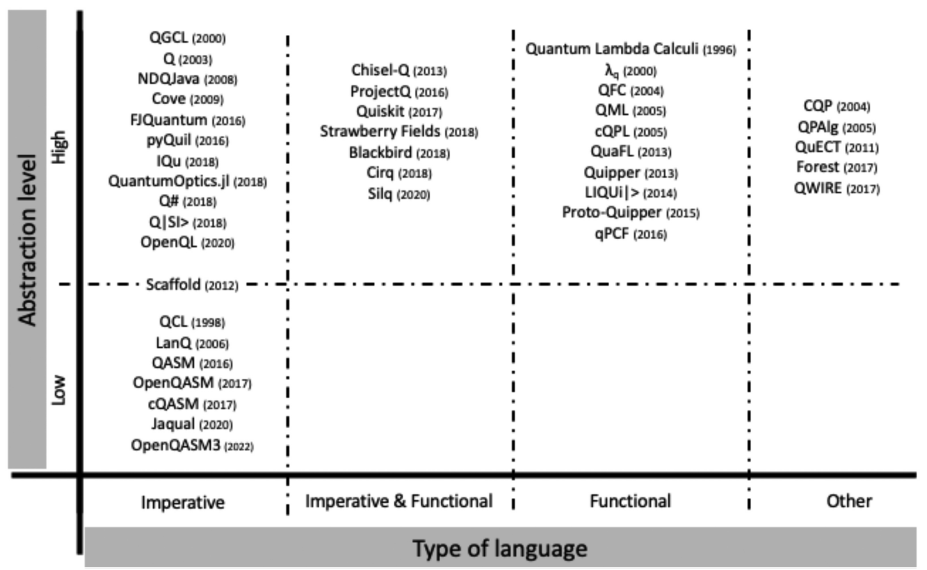
\includegraphics[width=1\linewidth]{images/quantum-programming/Quantum-Programming-Landscape.png}
    \caption{Übersicht über Quanten-Programmiersprachen nach Abstraktionsebenen und Programmierparadigmen. (Quantum Software Components and Platforms: Overview and Quality Assessment)}
    \label{fig:quantum-landscape}
\end{figure}

\paragraph{Hardwarebindung}
Die Hardwarebindung einer Quanten-Programmiersprache oder eines Frameworks beschreibt, inwieweit sie an eine bestimmte Quantenhardware-Plattform gebunden ist. Man unterscheidet zwischen Hardware-spezifisch und Hardware-unabhängig.

Hardware-Spezifische Frameworks sind für die Optimierung und Ausführung auf einer bestimmten Architektur konzipiert und optimiert. Sie nutzen die spezifischen Eigenschaften und Einschränkungen der Hardware zur Maximierung der Leistung. Beispiele hierfür sind Cirq, optimiert für Google Sycamore Hardware (https://quantumai.google/cirq) oder PyQuil, optimiert für Rigetti´s Quantum Cloud Service. (https://www.rigetti.com/what-we-build).

Hardware-unabhängige Sprachen und Frameworks sind so konzipiert, dass sie auf einer Vielzahl von Hardware-Plattformen ausgeführt werden können, oft durch die Verwendung von Zwischenrepräsentationen wie OpenQASM. Sie bieten eine große Flexibilität und Portabilität. Zu ihnen gehören unter anderem Qiskit von IBM sowie Q\# von Microsoft.

\paragraph{Quantenmodell} 
Eine weitere wesentliche Klassifikationsdimension ergibt sich aus dem zugrunde liegenden Quantenmodell. Quantencomputer können auf verschiedenen physikalischen Prinzipien und Berechnungsmodellen basieren, die sich auch in den Programmiersprachen widerspiegeln. Hierfür werden Programmiersprachen den Modellen aus \ref{programming-models} zugeordnet.

Das Gate-basierte Modell ist das dominanteste und am weitesten verbreitete Modell, bei dem Quantenalgorithmen durch Schaltkreise aus Quantengattern auf Qubits dargestellt werden. Ein Großteil der aktuellen Quantencomputer und Frameworks basieren auf diesem Modell. Beispiele für Sprachen und Frameworks sind die bereits erwähnten Qiskit, Cirq oder OpenQASM. 

Das messungsbasierte Paradigma (MBQC) führt Berechnungen durch eine Sequenz von Einzel-Qubit-Messungen auf einem vorbereiteten hochgradig verschränkten Anfangs-Cluster-Zustand durch. Die Wahl der Messbasis für jedes Qubit hängt hierbei von den Ergebnissen früherer Messungen ab. Bisher gibt es wenige produktive Frameworks, ein prominentes Beispiel ist jedoch der One-Way Quantum Computer. One-way (Einweg) ergibt sich daraus, dass jede Messung den Zustand eines Qubits zerstört und die Ressource verbraucht. Raussendorf et al. bewiesen, dass mithilfe eines zweidimensionalen Cluster-Zustands beliebige Quantenalgorithmen realisiert werden können, wodurch dieses Modell formal als äquivalent zum Schaltkreis-Modell zu sehen ist. (Measurement-based quantum computation)

Das adiabatische Paradigma nutzt Annealing zur Lösung komplexer Optimierungs- und Sampling-Probleme. Das bekannteste Beispiel hierfür ist das D-Wave Ocean SDK, das speziell für adiabatische Quantencomputer entwickelt wurde. Annealing übertrifft das Gate-Modell bei Optimierungsproblemen, da es den erheblichen Vorverarbeitungsaufwand vermeidet, der mit Gate-basierten Ansätzen verbunden ist. Darüber hinaus ist es deutlich toleranter gegenüber Fehlern und Rauschen und auf die Größe von Unternehmensproblemen skalierbar. (Optimization Performance of QA and QAOA D-Wave)

\paragraph{Zusammenfassung} 
In dieser Arbeit wurden bisher unter dem Begriff „Quanten-Programmiersprachen und -Frameworks“ sowohl formale, eigenständige Programmiersprachen als auch softwareseitige Entwicklungsumgebungen und Bibliotheken zusammengefasst, die die Programmierung, Ausführung und Analyse von Quantenalgorithmen ermöglichen.

Obwohl sich diese Systeme in Aufbau und Fokus teilweise unterscheiden, verfolgen sie das gemeinsame Ziel der Bildung einer Schnittstelle zwischen Quantenalgorithmen und deren Ausführung auf Quantenhardware oder Simulationen. Um eine systematische Vergleichbarkeit zu gewährleisten, wurden sie gemeinsam betrachtet und entsprechend ihrer funktionalen Eigenschaften klassifiziert. (Sollte ich den Teil lieber an den Anfang schreiben???)

Die folgende Tabelle fasst die Klassifizierungen verschiedener beispielhafter Quanten-Programmiersprachen und Frameworks zusammen. Die Einordnung beruht hierbei auf verschiedenen Arbeiten von (Quellen: A Survey on Available Tools and Technologies Enabling Quantum Computing | An exploratory study on the usage of quantum programming | Quantum Programming Language: A Systematic Review of Research Topic and Top Cited Languages | Quantum Software Components and Platforms: Overview and Quality Assessment)

\begin{table}[H]
\centering
\footnotesize
\begin{tabular}{|p{1cm}|p{3cm}|p{2cm}|l|l|p{2cm}|p{2cm}|}
\hline
\textbf{Jahr} & 
\textbf{Quantum-Programmiersprache / Framework} & 
\textbf{Abstraktions-level} & 
\textbf{Paradigma} & 
\textbf{Hardwarebindung} & 
\textbf{Quantenmodell} & 
\textbf{Hostsprache} \\
\hline
2017 & Qiskit & High-Level & Hybrid & IBM Q & Gate-basiert & Python \\
\hline
2018 & Cirq & High-Level & Hybrid & Google Sycamore & Gate-basiert & Python \\
\hline
2018 & Q\# & High-Level & Hybrid & ... & ...& C\# \\
\hline
1998 & QCL & Low-Level & Imperativ & ... & ... & C \\
\hline
2000 & qGCL & High-Level & Imperativ & ... & ... & Pascal \\
\hline
2003 & Q & High-Level & Imperativ & ... & ... & C++ \\
\hline
2006 & LanQ & Low-Level & Imperativ & ... & ... & C \\
\hline
2012 & Scaffold & Low-Level & Imperativ & ... & ... & C / C++ \\
\hline
2017 & OpenQASM & Low-Level & Imperativ & ... & ... & Assembly Lanaguage \\
\hline
2016 & pyQuil & High-Level & Imperativ & ... & ... & Python \\
\hline
2018 & Strawberry Fields & High-Level & Hybrid & ... & ... & Python \\
\hline
2020 & Silq & High-Level & Hybrid & ... & ... & Python \\
\hline
2020 & OpenQL & High-Level & Imperativ & ... & ... & Python, C++ \\
\hline
2022 & OpenQASM3 & Low-Level & Imperativ & ... & ... & Assembly Lanaguage \\
\hline
1996 & Quantum Lambda Calculi & High-Level & Funktional & ... & ... & Lambda Calculus \\
\hline
2005 & QML & High-Level & Funktional & ... & ... & Haskell \\
\hline
2013 & Quipper & High-Level & Funktional & ... & ... & Haskell \\
\hline
2020 & Braket SDK & High-Level & Hybrid & Amazon & ... & Python \\




\hline
\end{tabular}
\caption{Erweiterter Vergleich von Quantum-Programmiersprachen und Frameworks}
\label{tab:quantum_languages_full}
\end{table}
tbd

\subsection{Vertiefung ausgewählter Frameworks / QISKIT}

\textbf{Wie ausführlich soll ich diesen Teil machen? Alle drei Sprachen/Frameworks oder nur eins davon (Qiskit als Grundlage für nachfolgenden Teil und am weitesten verbreitete)? Wie detailliert?}
\begin{itemize}
    \item \textbf{Qiskit SDK:} Umfangreiche Bibliotheken, Simulator, Backendsteuerung
    \item \textbf{Cirq:} Framework von Google für Schaltungsdesign und Simulation
    \item \textbf{Q\#:} Domänenspezifische Sprache von Microsoft
\end{itemize}

\subsubsection{Qiskit}
\begin{itemize}
            \item Open-Source-SDK für Quanteninformatik
            \item Python-basiert
            \item Unterstützt IBM Quantum Experience Hardware
            \item Umfangreiches Ökosystem von Tools und Plugins
            
        \end{itemize}
Architktur
\begin{itemize}
    \item \textbf{Mehrschichtige Architektur}
    \begin{itemize}
        \item \textbf{Terra}: Grundlegende Funktionalität für das Arbeiten mit Quantenschaltkreisen
        \begin{itemize}
            \item Schaltkreisdarstellung und -manipulation
            \item Transpiler für Optimierung und Übersetzung
            \item Backend-Schnittstellen für Simulation und Hardware-Ausführung
        \end{itemize}
        
        \item \textbf{Aer}: Hochleistungs-Simulatoren
        \begin{itemize}
            \item Unterstützt verschiedene Simulationstypen: Zustandsvektor, Dichtematrix, Stabilisator
            \item Ermöglicht Rauschsimulation
        \end{itemize}
        
        \item \textbf{Ignis}: Werkzeuge für Charakterisierung und Fehlerminderung
        \begin{itemize}
            \item Fehlercharakterisierung und -kalibrierung
            \item Fehlerminderungstechniken
        \end{itemize}
        
        \item \textbf{Aqua}: Algorithmen für verschiedene Anwendungsbereiche
        \begin{itemize}
            \item Chemie, Finanzen, Maschinelles Lernen, Optimierung
        \end{itemize}
    \end{itemize}
    
    \item \textbf{Abstrakte und konkrete Schaltkreise}
    \begin{itemize}
        \item Abstrakte Schaltkreise: Repräsentation von Quantenalgorithmen auf hoher Abstraktionsebene
        \item Konkrete Schaltkreise: Implementierung mit Standardbibliothek von Gates
        \item OpenQASM als Zwischensprache für Quantenschaltkreise
    \end{itemize}
    
    \item \textbf{Transpiler}
    \begin{itemize}
        \item Übersetzt und optimiert Schaltkreise für die Ziel-Hardware
        \item Arbeitet in mehreren Durchläufen mit verschiedenen Passes
        \item Wichtige Passes:
        \begin{itemize}
            \item Layout-Selektion: Mapping von logischen zu physischen Qubits
            \item Routing: Einfügen von SWAP-Gates für nicht direkt verbundene Qubits
            \item Optimierung: Zusammenfassen von Gates, Entfernen unnötiger Gates
            \item Dekomposition: Zerlegung komplexer Gates in elementare Gates
        \end{itemize}
    \end{itemize}
    
    \item \textbf{Primitives}
    \begin{itemize}
        \item Grundlegende Bausteine für Quantenberechnungen
        \item \texttt{Sampler}: Stichproben aus Quantenschaltkreisen ziehen
        \item \texttt{Estimator}: Erwartungswerte von Observablen schätzen
    \end{itemize}
\end{itemize}

Besonderheiten und Anwendung

\begin{itemize}
    \item \textbf{Dynamische Schaltkreise}
    \begin{itemize}
        \item Ermöglichen klassisch kontrollierte Quantenoperationen
        \item Unterstützen Mid-Circuit-Messungen und bedingte Operationen
        \item Wichtig für adaptive Algorithmen und Fehlerkorrektur
    \end{itemize}
    
    \item \textbf{Fehlerminderung}
    \begin{itemize}
        \item Verschiedene Techniken zur Reduzierung von Hardwarefehlern
        \item Zero-Noise Extrapolation
        \item Probabilistic Error Cancellation
        \item Dynamical Decoupling
    \end{itemize}
    
    \item \textbf{Anwendungsgebiete}
    \begin{itemize}
        \item Quantenchemie und Materialwissenschaft
        \item Optimierungsprobleme
        \item Maschinelles Lernen
        \item Finanzmathematik
    \end{itemize}
    
    \item \textbf{Ökosystem und Community}
    \begin{itemize}
        \item Über 6 Millionen Installationen, 300.000 pro Monat
        \item 500+ Mitwirkende, die meisten nicht von IBM
        \item 300+ Pakete im Python Package Index (PyPI) hängen von Qiskit ab
        \item Über 2.000 wissenschaftliche Arbeiten haben Qiskit verwendet
    \end{itemize}
\end{itemize}



\section{Entwicklung von Quantenalgorithmen}

\subsection{Überblick über den Entwicklungsprozess}
\begin{itemize}
    \item Ziel: Praktische Umsetzung eines Quantenalgorithmus (End-to-End)
    \item Typische Phasen:
    \begin{itemize}
        \item Problemformulierung (z.\,B. Suche, Optimierung, Simulation)
        \item Auswahl eines geeigneten Paradigmas
        \item Abbildung auf ein Quantenmodell
        \item Wahl geeigneter Sprache / Frameworks (z.\,B. Qiskit)
        \item Implementierung, Testing, Ausführung (lokal und cloudbasiert)
    \end{itemize}
\end{itemize}

\subsection{Quantum Software Stack}

Das Quantencomputing basiert auf einem mehrschichtigen Software-Stack, mit dem abstrakte Quantenalgorithmen auf Quantenhardware übertragen und ausgeführt werden können. Eine mögliche Strukturierung eines solchen Software-Stacks ist in \autoref{fig:quantum-software-stack} abgebildet und setzt sich aus den drei Ebenen \emph{Nutzer (User Layer)}, \emph{Plattform (Platform Layer)} und \emph{Hardware (Hardware Layer)} zusammen. Jede dieser Schichten übernimmt spezifische Aufgaben innerhalb des Gesamtsystems und abstrahiert die Komplexität der darunterliegenden Ebenen.
\\
\paragraph{Nutzer}  
In der obersten Schicht werden Problemstellungen mittels Quantenalgorithmen (\autoref{basic_algorithms}) in konkreten Anwendungscode übertragen. Sie umfasst Werkzeuge und Bibliotheken, mit denen Entwickler Quantenalgorithmen und -anwendungen implementieren und für die Ausführung auf Quantenhardware vorbereiten können. Dazu gehören vor allem die in \autoref{sec:programming-languages} näher erläuterten Programmiersprachen und Entwicklungswerkzeuge (SDKs und Frameworks) wie Qiskit, Cirq oder Q\#.
\\
\paragraph{Plattform}  
Die Plattformschicht ist für die Kompilierung und Optimierung von Quantenprogrammen zuständig. Dazu gehören Compiler wie TKET oder der Qiskit Transpiler, die den Programmcode in Quantenhardware-kompatible Befehle übersetzen. Dazu zählen z.B. Gate-Dekomposition, Qubit-Zuordnung und Optimierung hinsichtlich Laufzeit und Fehlerresistenz. Auch dedizierte Software zur Fehlerkorrektur wie Riverlane kann dieser Schicht zugeordnet werden. Darüber hinaus enthält die Plattformschicht Simulatoren und Emulatoren wie Qiskit Aer oder Intel Quantum Simulator. Dabei handelt es sich um Software, die echte Quantenhardware nachbildet und so ein einfacheres Testen, Debuggen und Optimieren von Quantenanwendungen ermöglicht.
\\
\paragraph{Hardware}  
Am unteren Ende des Software-Stacks befindet sich die eigentliche Quantenhardware (Quantum Processing Unit) sowie Software für deren Verwaltung und Überwachung. Kontrollsysteme wie Quantum Machines OPX+ ermöglichen beispielsweise die Kalibrierung, Pulsgenerierung und qubitgenaue Steuerung der Hardware. Außerdem umfasst die Hardwareschicht weitere Fehlerkorrekturmechanismen.
\\
\\
Jede Schicht im Software-Stack abstrahiert technische Details der darunterliegenden Ebene und trägt zur strukturierten Entwicklung, Optimierung und Ausführung von Quantenprogrammen bei. \autocite{shehata_building_2025} \autocite{ryan_understanding_2024}

\begin{figure}[ht!]
\centering
\begin{tikzpicture}[
  layerbox/.style={
    draw,
    minimum width=6cm,
    minimum height=0.8cm,
    text centered
  }
]

\node[layerbox] (l1) at (0,  0) {Programmiersprachen};
\node[layerbox] (l2) at (0, -1) {SDKs und Frameworks};
\node[layerbox] (l3) at (0, -2) {Quantenalgorithmen};
\node[layerbox] (l4) at (0, -3) {Quantenanwendungen};

\node[layerbox] (l5) at (0, -4.5) {Simulation};
\node[layerbox] (l6) at (0, -5.5) {Kompilierung};
\node[layerbox] (l7) at (0, -6.5) {Fehlerkorrektur};

\node[layerbox] (l8) at (0, -8) {Kontrollsysteme};
\node[layerbox] (l9) at (0, -9) {Quantum Processing Unit (QPU)};

\draw[decorate, decoration={brace, amplitude=6pt, mirror}, very thick]
  ($(l1.north west) + (-0.2,0.1)$) -- ($(l4.south west) + (-0.2,-0.1)$)
  node[midway, xshift=-0.4cm, anchor=east, font=\normalsize\bfseries] {Nutzer};

\draw[decorate, decoration={brace, amplitude=6pt, mirror}, very thick]
  ($(l5.north west) + (-0.2,0.1)$) -- ($(l7.south west) + (-0.2,-0.1)$)
  node[midway, xshift=-0.4cm, anchor=east, font=\normalsize\bfseries] {\textbf{Plattform}};

\draw[decorate, decoration={brace, amplitude=6pt, mirror}, very thick]
  ($(l8.north west) + (-0.2,0.1)$) -- ($(l9.south west) + (-0.2,-0.1)$)
  node[midway, xshift=-0.4cm, anchor=east, font=\normalsize\bfseries] {\textbf{Hardware}};

\end{tikzpicture}
\caption{Struktur eines Quantum Software-Stacks \autocite{ryan_understanding_2024}}
\label{fig:quantum-software-stack}
\end{figure}

\textbf{Näher eingehen auf Compiler und Simulator?}

\subsection{Quantum Cloud Computing}

Die in der untersten Schicht des Quantum Software-Stacks befindliche Quantenhardware ist teuer in der Anschaffung und komplex zu betreiben. Das Konzept des Quantum Cloud Computing (QCC) zielt darauf ab, Endnutzern den Zugang zu Quantenhardware über Cloud-Plattformen zu erleichtern. Diese bieten Zugang zu Ressourcen, Jobmanagement und Fehlermitigation mittels abstrahierter Schnittstellen in einer skalierbaren Umgebung.

Ein zentraler Vorteil Cloud-basierter Quantenplattformen liegt in ihrer Flexibilität: Nutzer können ihre Rechenkapazitäten bedarfsgerecht skalieren, was die Bearbeitung unterschiedlich komplexer Probleme effizienter gestaltet. Außerdem ermöglichen sie das einfache Entwickeln und Testen von Quantenalgorithmen in simulierten Umgebungen, bevor diese auf echter Hardware ausgeführt werden. Dies reduziert die Einstiegshürden, da keine spezialisierte Infrastruktur oder tiefgreifende Hardwarekenntnisse notwendig sind. Da alle Nutzer auf dieselbe Plattform zugreifen, werden darüber hinaus globale Kollaboration und standardisierte Entwicklungsumgebungen begünstigt.

Zu den wichtigsten Anbietern von Quantum Cloud Plattformen zählen aktuell IBM, Amazon und Google. Ihre Plattformen IBM Quantum\footnote{IBM Quantum \url{https://quantum.ibm.com/}}, Amazon Braket\footnote{Amazon Braket \url{https://aws.amazon.com/braket/}} und Google Quantum AI\footnote{Google Quantum AI \url{https://quantumai.google/cirq/google/concepts}} sind in \autoref{tab:quantum-cloud-platforms} gegenübergestellt \autocite{trends+challenges-TODO-sync}.

\begin{table}[ht!]
\centering
\begin{tabular}{|p{2.5cm}|p{4.8cm}|p{4cm}|}
\hline
\textbf{Plattform} & \textbf{Hardware} & \textbf{Unterstützte Sprachen / SDKs} \\
\hline
IBM Quantum & Falcon, Eagle (Supraleitende Qubits) & Qiskit \\
\hline
Amazon Braket & IonQ (Ionenfallen), Rigetti (supraleitend), OQC (Photonik) & Braket SDK, PennyLane, Qiskit \\
\hline
Google Quantum AI & Sycamore (supraleitend) & Cirq \\
\hline
\end{tabular}
\caption{Vergleich führender Quantum Cloud Plattformen}
\label{tab:quantum-cloud-platforms}
\end{table}

Alle drei Plattformen bieten Cloud-basierten Zugang zu Quantenprozessoren im Pay-as-you-go-Modell, wodurch Nutzer ohne hohe Einstiegskosten reale Quantenhardware nutzen können. Dabei unterstützen alle Anbieter hybride Workflows, bei denen klassische und quantenbasierte Berechnungen kombiniert werden. Angesichts der Fehleranfälligkeit heutiger Quantenhardware integrieren alle Plattformen Mechanismen zur Fehlermitigation. Zudem sind alle Plattformen gut in ihre jeweiligen Cloud-Ökosysteme integriert (IBM Cloud, AWS, Google Cloud), um Nutzern eine nahtlose Entwicklung und Verwaltung quantenbasierter Anwendungen zu ermöglichen.

Die drei Plattformen unterscheiden sich vor allem in der Hardwareverfügbarkeit, Softwarearchitektur und ihrem Ausführungsmodell. IBM Quantum bietet exklusiv Zugang zu eigenen supraleitenden Quantenprozessoren, darunter fortschrittliche Geräte wie den 127-Qubit-Eagle. Amazon Braket hingegen fungiert als Meta-Plattform und stellt über eine einheitliche Schnittstelle Zugang zu verschiedenartigen QPUs bereit – z.B. Ionenfallen (IonQ) und supraleitende Systeme (Rigetti, OQC). Google Quantum AI verwendet ausschließlich eigene supraleitende Chips (z.B. Sycamore), die jedoch nur ausgewählten Partnern zugänglich sind. Damit bieten IBM und AWS aktuell breiteren öffentlichen Hardwarezugang, während Google auf forschungsorientierte Hardwareentwicklung mit begrenztem Zugriff setzt.

Auch auf Softwareebene gibt es Unterschiede: IBM unterstützt mit Qiskit ein umfassendes Open-Source SDK. Braket erlaubt mehr Flexibilität, indem es neben dem eigenen SDK auch Drittanbieter-Frameworks wie PennyLane unterstützt. Google verwendet Cirq – ein eher Low-Level-orientiertes SDK, das präzise Kontrolle über qubit-spezifische Details ermöglicht, insbesondere im Kontext von Machine Learning mit TensorFlow Quantum. Bei den Ausführungsmodellen bietet IBM mit Qiskit Runtime ein latenzarmes Session-Modell inklusive dynamischer Schaltungen, während Braket hybride Jobs in AWS-Containern orchestriert. Google hingegen ermöglicht primär Batch-Ausführungen über das Quantum Engine API – ohne öffentliche Hybrid-Job-Funktionalität.

Darüber hinaus gibt es weitere Plattformen wie etwa \textit{Strangeworks}, \textit{Xanadu}, \textit{Quantinuum}, \textit{IonQ} (auch über Azure Quantum) und \textit{Microsoft Azure Quantum}. Diese bieten entweder eigene Hardwaretechnologien (wie photonische QPUs bei Xanadu oder trapped-ion Systeme bei Quantinuum) oder bündeln übergreifende Multi-Backend-Zugänge mit einheitlicher API. Microsoft ermöglicht zudem tiefe Integration in klassische Azure-Dienste, während Strangeworks auf eine benutzerfreundliche Multi-Vendor-Umgebung setzt.

\subsection{Tooling und Automatisierung}
\begin{itemize}
    \item Transpiler: Anpassung an spezifisches Backend
    \item Middleware: Warteschlange, Priorisierung, Job-IDs
    \item Backend-Optimierung: z.\,B. minimale Tiefe, minimale Fehlerwahrscheinlichkeit
    \item Möglichkeit automatisierter Testausführung mit Simulator
\end{itemize}

\subsection{Praxisbeispiel: Grover-Suche mit Qiskit} 
Dieses Beispiel veranschaulicht die praktische Umsetzung des Grover-Algorithmus zur Lösung eines unstrukturierten Suchproblems. Der Algorithmus zielt darauf ab, in einem Zustandsraum mit $2^n$ Einträgen einen bestimmten, zuvor markierten Zustand mit signifikant weniger Abfragen zu identifizieren, als dies klassisch möglich wäre. Die Implementierung erfolgt auf Grundlage eines gate-basierten Quantenmodells, wobei zunächst einfache Systeme mit zwei und drei Qubits betrachtet werden.

Ausgangspunkt ist jeweils ein Qubit-Register, das durch die Anwendung von Hadamard-Gattern in eine gleichmäßige Superposition aller möglichen Zustände überführt wird. Diese Phase der Initialisierung erzeugt einen quantenmechanischen Zustand, in dem jeder mögliche Eintrag des Suchraums mit gleicher Amplitude repräsentiert ist. Der nächste Schritt besteht in der Anwendung des sogenannten Orakels, das den gesuchten Zustand durch eine Phaseninversion markiert. In der hier realisierten Version wird im Fall von zwei Qubits der Zustand $|11\rangle$ als Zielzustand definiert und durch ein einfaches CZ-Gatter identifiziert. Für die Erweiterung auf drei Qubits wird entsprechend ein mehrfach kontrolliertes Z-Gatter eingesetzt, das gezielt den Zustand $|111\rangle$ anspricht.

Im Anschluss an das Oracle kommt der sogenannte Diffusionsoperator zur Anwendung, der eine Spiegelung aller Amplituden um ihren Mittelwert bewirkt. Ziel dieses Schritts ist es, die Wahrscheinlichkeit des markierten Zustands zu verstärken, während die übrigen Zustände unterdrückt werden. Die Umsetzung erfolgt durch eine festgelegte Folge elementarer Gatter, darunter Hadamard-, X- und kontrollierte NOT-Gatter. Schon nach einer einzigen Iteration dieses Verfahrens – bei kleinen Registern in der Regel ausreichend – ist der Zielzustand in der quantenmechanischen Wahrscheinlichkeitsverteilung deutlich hervorgehoben.

Die finale Messung der Qubits erfolgt am Ende des Algorithmus. Dabei zeigt sich, dass der zuvor markierte Zustand mit hoher Wahrscheinlichkeit detektiert wird. Die experimentelle Auswertung bestätigt die theoretische Erwartung: Der Grover-Algorithmus führt zu einer gezielten Verstärkung des gewünschten Ergebnisses. Dies wird insbesondere durch die grafische Darstellung der Messhäufigkeiten deutlich, bei der der Zielzustand als klar dominanter Messwert erscheint.

Insgesamt zeigt dieses Beispiel, wie sich ein komplexer quantenmechanischer Algorithmus mit relativ einfachen Mitteln umsetzen lässt. Die Verbindung von Theorie und Praxis wird damit greifbar: Während im Kapitel Quantenalgorithmen die mathematische Grundlage gelegt wurde, bietet die hier vorgestellte Implementierung eine konkrete Anwendung und liefert gleichzeitig einen Einstieg in den praktischen Umgang mit modernen Quantenentwicklungstools.

\subsection{Implementierung und Testing mit Qiskit}
\subsubsection{Projektstruktur und Setup (Python-Umgebung, Qiskit-Installation)}

\setlength{\parindent}{0pt} % Keine Einrückung am Absatzanfang
\setlength{\parskip}{1em}   % Fügt einen vertikalen Abstand von 1em zwischen Absätzen ein

\subsubsection*{Systemanforderungen}
Die Systemanforderungen für die Implementierung und das Testing mit Qiskit sind wie folgt:
\begin{itemize}
    \item \textbf{Betriebssystem}: Windows 10 oder 11 (64-Bit)
    \item \textbf{Python-Version}: Python 3.8 bis 3.11
    \item \textbf{Arbeitsspeicher}: Mindestens 4 GB RAM (empfohlen: 8 GB oder mehr)
    \item \textbf{Festplattenspeicher}: Ca. 1--2 GB freier Speicherplatz
    \item \textbf{Internetverbindung}: Für Installation, Updates und IBM-Zugriff
\end{itemize}

\subsubsection*{Virtuelle Umgebung und Qiskit installieren}

\begin{enumerate}
    \item \textbf{Virtuelle Umgebung einrichten} 
    
Virtuelle Umgebungen helfen dabei, Abhängigkeiten eines Projekts zu isolieren und Konflikte mit anderen Projekten zu vermeiden.
    \begin{verbatim}
python -m venv C:\Users\deinBenutzername\Documents\quantum-env
    \end{verbatim}
\textit{Dieser Befehl erstellt eine neue virtuelle Python-Umgebung im angegebenen Verzeichnis, wodurch alle Projektabhängigkeiten lokal isoliert gespeichert werden. }
   

 \item \textbf{Virtuelle Umgebung aktivieren}
    \begin{verbatim}
cd C:\Users\deinBenutzername\Documents\quantum-env
.\Scripts\activate
    \end{verbatim}
\textit{Diese Befehle wechseln in das Verzeichnis der virtuellen Umgebung und aktivieren sie.  Der Prompt zeigt danach den Namen der aktiven Umgebung an, was ein Zeichen dafür ist, dass alle weiteren Befehle lokal ausgeführt werden. }
  

    \item \textbf{pip-Version prüfen}
    \begin{verbatim}
pip --version
    \end{verbatim}
\textit{Dieser Befehl überprüft, ob der Python-Paketmanager \texttt{pip} korrekt installiert und aktiviert ist.  \texttt{pip} wird im nächsten Schritt zur Installation der Pakete verwendet. }
    
\end{enumerate}

\subsubsection*{Installation der benötigten Pakete}

\begin{enumerate}
    \setcounter{enumi}{3} % Zähler für fortlaufende Liste
    \item \textbf{Qiskit installieren}
    \begin{verbatim}
pip install qiskit
    \end{verbatim}
\textit{Dieser Befehl installiert das Hauptpaket \texttt{qiskit}, das alle grundlegenden Funktionen zur Programmierung und Simulation von Quantencomputern enthält. }

    \item \textbf{Visualisierungsfunktionen hinzufügen (optional, empfohlen)}
    \begin{verbatim}
pip install qiskit[visualization]
    \end{verbatim}
\textit{Dieser Befehl installiert zusätzliche Bibliotheken zur grafischen Darstellung von Quanten-Schaltkreisen und Simulationsergebnissen, z.B. mit Matplotlib.  Dies ist notwendig bei Nutzung von Jupyter Notebook. }

    \item \textbf{IBM Runtime installieren (optional)}
    \begin{verbatim}
pip install qiskit-ibm-runtime
    \end{verbatim}
\textit{Dieser Befehl ermöglicht die Anbindung an echte Quantenhardware über IBMs Cloud-Umgebung.  Dies ist optional, aber hilfreich für fortgeschrittene Experimente. }
\end{enumerate}

\subsubsection*{Jupyter Notebook nutzen}

\begin{enumerate}
    \setcounter{enumi}{6} % Zähler für fortlaufende Liste
    \item \textbf{Jupyter installieren}
    \begin{verbatim}
pip install jupyter
    \end{verbatim}
\textit{Dieser Befehl installiert Jupyter Notebook -- eine interaktive Umgebung, in der Python-Code, Visualisierungen und Textelemente kombiniert werden können. }


    \item \textbf{Notebook starten}
    \begin{verbatim}
jupyter notebook
    \end{verbatim}
\textit{Dieser Befehl startet den Jupyter Notebook-Server und öffnet die Benutzeroberfläche im Webbrowser.  Hier können direkt interaktive Codebeispiele mit Qiskit ausgeführt werden. }

\end{enumerate}

\subsubsection{Konstruktion des Grover Circuits:}


Um den Grover Algorithmus praktisch auf eine Quantencomputer umzusetzen, wird eine konkrete Konstruktion der Schaltung benötigt. Der Algorithmus setzt sich dabei aus 4 wesentlichen Komponenten zusammen: 
\begin{enumerate}
    \item  Initialisierung: Hierbei werden die Qubits in eine gleichmäßige Superposition gebracht
    \item Oracle: Im Oracle wird der gesuchte Zustand, welcher der Grover Algorithmus identifizieren soll, ausgewählt
    \item Diffusionsoperator: Der Diffusionsoperator verstärkt den Zustand des Oracle
    \item   Messung: Abgeschlossen wird der Algorithmus mit der Messung, um das Ergebnis zu erhalten. 
\end{enumerate}

Diese 4 Schritte können beliebig für eine beliebige Anzahl an Qubits angewendet werden. Im Folgenden werden die 4 Komponenten nochmals ausführlicher beschrieben. Das Ganze erfolgt jeweils mathematisch, konzeptionell und zusätzlich noch praktisch. Für den praktischen Teil wurde ein Grover Algorithmus mit Qiskit in Jupyter Notebooks implementiert und Codeausschnitte zeigen Schritt für Schritt die praktische Umsetzung.

\subsection*{Initialisierung}
Der Startzustand aller Qubits ist $\ket{0}$. Um eine gleichverteilte Superposition über alle Basiszustände der Qubits zu erzeugen, muss für jedes der Qubits ein Hadamard-Gate ($H$) angewendet werden. Für die Anzahl $n$ Qubits ergibt sich daraus folgender Zusammenhang:
$$
|\psi_0\rangle = H^{\otimes n}|0\rangle^{\otimes n} = \frac{1}{\sqrt{2^n}} \sum_{x=0}^{2^n-1} |x\rangle
$$
Der beschriebene Zustand bildet die Grundlage für die Amplitudenverstärkung von Grovers Algorithmus. Jede Lösung hat damit zunächst dieselbe Wahrscheinlichkeit. (vgl. \citeauthor{nielsen_quantum_2010}, \citeyear{nielsen_quantum_2010}, S.257)

Mit Qiskit in Jupyter Notebooks wird zunächst die `QuantumCircuit`-Bibliothek benötigt. Anschließend kann die Initialisierung, also der Ausgangspunkt für jeden Grover-Algorithmus, wie folgt in Qiskit umgesetzt werden:
\subsection*{Beispiel für 2 Qubits:}
\begin{verbatim}
from qiskit import QuantumCircuit

# Quantenschaltung mit 2 Qubits und 2 klassischen Bits erstellen
qc = QuantumCircuit(2, 2)

# Hadamard-Gate auf jedes Qubit anwenden
qc.h([0, 1])


\end{verbatim}


Das gewählte Beispiel ist für 2 Qubits, kann jedoch, wie bereits erwähnt, für die Anzahl $n$ Qubits beliebig erweitert werden.

\subsection*{Oracle}
Der nächste Schritt in der Implementierung des Grover-Algorithmus nennt sich Oracle. Bei Oracle handelt es sich um eine unitäre Operation $U_f$, welche den gesuchten Zustand $\ket{T}$ durch eine Phaseninversion der Qubits kenntlich macht. Das bedeutet, dass in diesem Schritt immer der gesuchte Zielzustand markiert wird. Dies erlaubt im Beispiel von 2 Qubits vier verschiedene Zielzustände: "00", "01", "10" und "11".

Dieser Zusammenhang wird wie folgt beschrieben:
$$
U_f \ket{x} = (-1)^{f(x)} \ket{x}
$$
Ein ideales Oracle wird formal wie folgt beschrieben:
$$
U_f \ket{x} = \begin{cases} -\ket{x} & \text{wenn } x \text{ der gesuchte Zustand ist} \\ \ket{x} & \text{sonst} \end{cases}
$$
Für die Standardversion des Grover-Algorithmus wird der Parameter $f(x)$ in der genannten Formel gesetzt, was zu folgender Formel führt:
$$
U_f \ket{x} = (-1)^{\delta_{x,T}} \ket{x}
$$
Die daraus entstehende Inversion lässt sich als eine Reflexion des Zustandsvektors im sogenannten Hilbertraum interpretieren. (Roy et al 2022, Grover 1996)

Zum besseren Verständnis, wie das Genannte mit Qiskit in Jupyter Notebooks umgesetzt wird, hier die Fortsetzung des Beispiels für 2 Qubits. Als Beispiel wird im Folgenden nun der Zielzustand $\ket{01}$ markiert.

Standardmäßig wirkt das CZ-Gate (Controlled-Z Gate) in Qiskit auf den Zustand $\ket{11}$. Wenn man nun einen der anderen genannten Zustände markieren möchte, muss man mit NOT-Gates (X-Gates) arbeiten, welche die Qubits so transformieren, dass der gewünschte Zielzustand vor dem CZ-Gate zum Zustand $\ket{11}$ wird und nach dem CZ-Gate wieder zurücktransformiert wird.

\subsection*{Zielzustand $\ket{01}$ markieren (Beispiel):}
Um den Zustand $\ket{01}$ zu markieren, invertieren wir das erste Qubit (Index 0) mit einem X-Gate, sodass aus $\ket{0}$ ein $\ket{1}$ wird. Das zweite Qubit (Index 1) bleibt $\ket{1}$. Somit wird aus $\ket{01}$ ein $\ket{11}$. Anschließend wenden wir das CZ-Gate an und invertieren das erste Qubit wieder zurück, um den Zustand wiederherzustellen.

\begin{verbatim}
# Oracle für den Zielzustand |01> erstellen
# Qubit 0 (links) ist 0, Qubit 1 (rechts) ist 1
# Um aus |01> ein |11> zu machen, muss Qubit 0 invertiert werden (X-Gate)

# X-Gate auf Qubit 0 anwenden (0 -> 1)
qc.x(0)
# CZ-Gate anwenden (wirkt auf |11>)
qc.cz(0, 1)
# X-Gate auf Qubit 0 zurückanwenden (1 -> 0)
qc.x(0)

# Schaltung zeichnen (optional)
# qc.draw('mpl')
\end{verbatim}
Mit dieser Vorgehensweise können beliebige Zielzustände auf einfache Weise realisiert werden, und das Ganze ohne zusätzliche Hilfs-Qubits. Das funktioniert auch für die Anzahl $n$ Qubits. 
(vgl. \citeauthor{roy_deterministic_2022}, \citeyear{roy_deterministic_2022})



\subsection*{Diffusionsoperator}
Der Diffusionsoperator, welcher auch häufig „Inversion about the mean“ genannt wird, verstärkt den im Oracle markierten Zielzustand, indem er alle Amplituden am Mittelwert reflektiert. Die Definition des Diffusionsoperators ist folgende:
$$
D = 2|\psi\rangle\langle\psi| - I
$$
Dabei steht der Parameter $|\psi\rangle$ für den gleichverteilten Zustand. Das entspricht aus geometrischer Sicht einer Spiegelung im Hilbertraum. Genau diese Operation ist für die Verstärkung des im Oracle markierten Zielzustands verantwortlich. Nach jeder Grover-Iteration bewirkt sie eine Rotation des Zustandsvektors um einen festen Winkel im Unterraum von markierten und unmarkierten Zuständen. (vgl. Grover 1996, Montanaro 2016).

In unserem gewählten Beispiel mit 2 Qubits kann der Diffusionsoperator in Qiskit wie folgt umgesetzt werden:
\begin{verbatim}
grover_circuit.h([0,1])   # Rücktransformation in H-Basis
grover_circuit.z([0,1])   # Phaseninversion aller Zustände
grover_circuit.cz([0,1])  # Inversion von |00> in H-Basis
grover_circuit.h([0,1])   # Zurück in ursrüngliche Basis
\end{verbatim}

Optional kann das auch mit dem `GroverOperator` aus der Qiskit-Bibliothek gelöst werden. Dieser kapselt Oracle und Diffusion und wird wie folgt umgesetzt:
\begin{verbatim}
from qiskit.circuit.library import GroverOperator
grover_op = GroverOperator (oracle=oracle)
\end{verbatim}

\subsection*{Messung}
Der abschließende Schritt im Grover Algorithmus ist die Messung. Diese folgt nach mehreren Iterationen von Oracle und Diffusion (typischerweise $\approx \frac{\pi}{4} \sqrt{2^n}$)
\begin{verbatim}
grover_circuit.measure_all()
\end{verbatim}
Diese überführt den quantenmechanischen Zustand in einen klassischen Bitstring. 
Die Wahrscheinlichkeit, bei der Messung den markierten Zustand zu erhalten ist nun maximal. Bei Benutzung der Simulation erfolgt diese Messung häufig mehrfach in sogenannten „shots“, um eine Wahrscheinlichkeitsverteilung zu erhalten. So lässt sich die Dominanz des gesuchten Zustands gegenüber der anderen Zustände statistisch nachweisen.

Die Konstruktion des Grover-Circuits ist modular und besteht wie beschrieben aus den genannten vier klar definierten Schritten. Mithilfe von Qiskit lassen sich diese Schritte präzise implementieren, debuggen und simulieren. Das kann sowohl für die theoretische Analyse als auch für praktische Experimente auf realen Quantencomputern verwendet werden.

(vgl. \citeauthor{ibm_quantum_nodate}, \citeyear{ibm_quantum_nodate}; vgl. \citeauthor{noauthor_grovers_nodate}, \citeyear{noauthor_grovers_nodate})
\subsubsection{Ausführung auf Simulator (Qiskit Aer)}
\subsubsection{Visualisierung von Schaltkreis und Ergebnissen}

\setlength{\parindent}{0pt} % Keine Einrückung am Absatzanfang
\setlength{\parskip}{1em}   % Fügt einen vertikalen Abstand von 1em zwischen Absätzen ein

Ein zentrales Anliegen beim Verständnis und bei der Vermittlung von Quantenalgorithmen ist die Möglichkeit, deren Funktionsweise nicht nur abstrakt-mathematisch, sondern auch visuell nachvollziehen zu können. Das folgende Kapitel widmet sich der Visualisierung des Grover-Algorithmus anhand zweier Implementierungen – einmal mit zwei, einmal mit drei Qubits – unter Verwendung des Qiskit-Frameworks. Sowohl der Aufbau des Quanten-Schaltkreises als auch die Messergebnisse werden grafisch dargestellt und interpretiert.

\paragraph*{Visualisierung des Quantenschaltkreises}
\mbox{}

Für beide Varianten des Grover-Algorithmus wird der jeweilige Quanten-Schaltkreis mit der Methode QuantumCircuit.draw() visualisiert. Diese Darstellung erlaubt einen direkten Einblick in den logischen Aufbau des Algorithmus, insbesondere in die Abfolge und Wirkung der verschiedenen quantenmechanischen Operationen. Die Schaltkreise bestehen jeweils aus mehreren charakteristischen Abschnitten:
\begin{itemize}
    \item \textbf{Initialisierung:} Alle Qubits werden im Zustand $\ket{0}$    vorbereitet.
    \item \textbf{Superposition:} Durch Anwendung von Hadamard-Gattern wird eine gleichmäßige Überlagerung aller möglichen Basiszustände erzeugt.
    \item \textbf{Oracle:} Eine gezielte Phaseninversion kennzeichnet den gesuchten Zustand. Dieser Schritt implementiert die sogenannte „Markierung“ des Zielzustands.
    \item \textbf{Diffusion (Grover-Operator):} In einem weiteren Schritt wird der markierte Zustand durch Interferenz verstärkt. Dies geschieht durch Spiegelung an der Mittelwertachse aller Amplituden.
    \item \textbf{Messung:} Zum Abschluss des Algorithmus erfolgt eine Messung aller Qubits.
\end{itemize}
\noindent
Die nachstehenden Codeausschnitte zeigen, wie die Schaltkreise für beide
Varianten im Notebook erzeugt und angezeigt werden:

\begin{verbatim}
circuit.draw()
\end{verbatim}

  \begin{figure}
      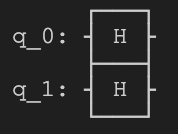
\includegraphics[width=0.25\linewidth]{circuit_superposition.png}
      \caption{Visualisierung des Schaltkreises (Superposition)}
      \label{fig:enter-label}
\end{figure}

\paragraph*{Visualisierung der Messergebnisse}
\mbox{}

Nach Ausführung des Algorithmus auf einem Quantensimulator – konkret dem QASM-Simulator von Qiskit – erfolgt die Analyse der Ergebnisse durch grafische Darstellung der Messausgänge.  Dabei wird die Methode \texttt{plot\_histogram()} verwendet, die ein Histogramm der gemessenen Zustände erzeugt.  Die Höhe der jeweiligen Balken repräsentiert die Häufigkeit (bzw. Wahrscheinlichkeit) eines bestimmten Bitmusters, das bei der Messung beobachtet wurde. 

Im Idealfall – das heißt, bei korrekter Funktionsweise des Orakels und des Grover-Operators – zeigt das Histogramm einen klar dominanten Peak beim Zielzustand.  Die Wahrscheinlichkeiten für alle anderen Zustände bleiben deutlich geringer.  Der gesuchte Zustand hebt sich somit durch quantenmechanische Verstärkung deutlich ab.  Der entsprechende Code zur Ergebnisvisualisierung lautet: 
\begin{verbatim}
plot_histogram(counts)
plt.show()
plot_histogram(counts)
plt.show()
\end{verbatim}

\begin{figure}
    \centering
    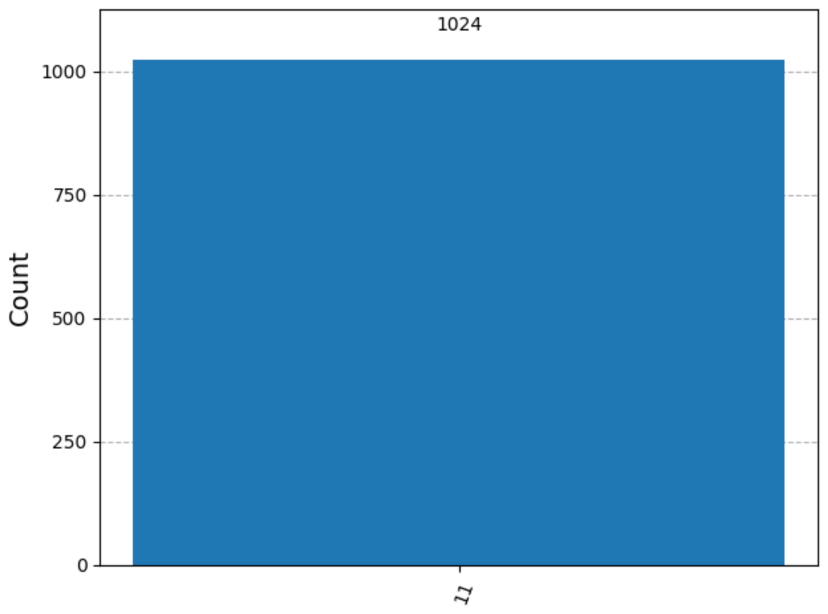
\includegraphics[width=0.75\linewidth]{Visualisierung der Messergebnisse.png}
    \caption{Visualisierung der Messergebnisse}
    \label{fig:enter-label}
\end{figure}

Die Kombination aus Schaltkreisvisualisierung und Ergebnisdarstellung bietet einen idealen Zugang zum Verständnis von Grovers Algorithmus.  Sie macht die Wirkung der einzelnen quantenlogischen Schritte nachvollziehbar und veranschaulicht das Prinzip der amplitudenbasierten Suche auf anschauliche Weise.  Solche Visualisierungen sind nicht nur didaktisch wertvoll, sondern auch essenziell für die Entwicklung und Analyse komplexerer Quantenalgorithmen in der Praxis. 

\clearpage % Fügt einen Seitenumbruch ein, um den nächsten Abschnitt auf einer neuen Seite zu beginnen

\subsubsection{Tests und Debugging-Hilfsmittel (z.\,B. Histogramme, Counts)}


\paragraph*{Tests und Debugging-Hilfsmittel}
\mbox{}

Bei der Entwicklung von Quantenalgorithmen spielt die systematische Überprüfung des Codes eine entscheidende Rolle, insbesondere im experimentellen Rahmen mit Frameworks wie Qiskit. Quantenprogramme sind nicht nur aufgrund ihrer Komplexität fehleranfällig, sondern verhalten sich auch häufig nicht intuitiv, da viele Zustände nicht direkt beobachtbar sind. Deshalb ist es essenziell, gezielt mit Tests, Zwischenergebnissen und Visualisierungen zu arbeiten, um Fehler zu erkennen und zu beheben.

\paragraph*{Schrittweise Entwicklung und Visualisierung}
\mbox{}

Im vorliegenden Notebook wurde der Grover-Algorithmus schrittweise aufgebaut, was eine erste Form des \enquote{Testens durch Design} darstellt. So wurden zunächst einzelne Operatoren und Zustände erzeugt, bevor sie in die Gesamtschaltung integriert wurden. Ein typisches Beispiel findet sich im Abschnitt zur 2-Qubit-Version:
\begin{verbatim}
def diffusion(circuit):
    circuit.h([0, 1])
    circuit.x([0, 1])
    circuit.h(1)
    circuit.cx(0, 1)
    circuit.h(1)
    circuit.x([0, 1])
    circuit.h([0, 1])
# Grover Circuit
grover_circ = QuantumCircuit(2)
grover_circ.h([0, 1])         # Superposition
oracle(grover_circ)           # Oracle anwenden
diffusion(grover_circ)        # Verstärkung
grover_circ.measure_all()
def diffusion(circuit):
    circuit.h([0, 1])
    circuit.x([0, 1])
    circuit.h(1)
    circuit.cx(0, 1)
    circuit.h(1)
    circuit.x([0, 1])
    circuit.h([0, 1])
# Grover Circuit
grover_circ = QuantumCircuit(2)
grover_circ.h([0, 1])         # Superposition
oracle(grover_circ)           # Oracle anwenden
diffusion(grover_circ)        # Verstärkung
grover_circ.measure_all()
\end{verbatim}
Durch das schrittweise Ergänzen der Gates kann bereits in frühen Phasen kontrolliert werden, ob jede Transformation wie gewünscht wirkt. Dies entspricht einem iterativen Debugging-Verfahren.

\paragraph*{Visualisierung als Debugging-Werkzeug}
\mbox{}

Wie im vorherigen Kapitel gezeigt, wird mit \texttt{draw()} der Schaltkreis visualisiert. Dies erfüllt nicht nur dokumentarische, sondern auch diagnostische Zwecke. Es kann dadurch überprüft werden, ob etwa das Oracle korrekt umgesetzt oder die Anzahl der Grover-Iterationen richtig gewählt wurde.
\subparagraph*{Beispiel:}
\begin{verbatim}
circuit.draw()
circuit.draw()
\end{verbatim}
Fehlende oder falsch platzierte Gates werden so unmittelbar sichtbar. Besonders hilfreich ist dies bei komplexeren Operatorfolgen wie in der 3-Qubit-Version.

\paragraph*{Ergebnisanalyse durch Histogramme}
\mbox{}

Ein sehr effektives Mittel zur Fehlererkennung ist die statistische Analyse der Ausgaben. Die mit \texttt{plot\_histogram()} erzeugten Verteilungen lassen Rückschlüsse auf das Verhalten des Algorithmus zu:
\begin{verbatim}
plot_histogram(result.get_counts())
plot_histogram(result.get_counts())
\end{verbatim}
Tritt der erwartete Peak beim Zielzustand nicht auf, kann dies auf einen Fehler im Oracle, in der Grover-Iteration oder in der Initialisierung hinweisen. Wurde beispielsweise ein falsches CZ-Gatter verwendet oder versehentlich eine falsche Qubit-Reihenfolge angesprochen, so verteilt sich die Wahrscheinlichkeitsmasse ungleichmäßig oder falsch.

\paragraph*{Fazit}
\mbox{}

Die Arbeit mit Quantenalgorithmen erfordert sowohl eine sorgfältige Teststrategie, klassische Softwareentwicklung aber auch eine strukturiertere Herangehensweise. Im Notebook werden bereits einfache Mittel wie Visualisierung, gezielte Zwischenschritte und Histogrammanalyse genutzt und sind eine große Hilfe beim Debugging. Für komplexere Algorithmen empfiehlt sich darüber hinaus der gezielte Einsatz von Statevector-Simulationen, Barrieren zur Strukturierung und die Ausgabe von Zwischenzuständen.

\subsection{Fazit und Ausblick}
\begin{itemize}
    \item Zusammenfassung der Entwicklungsschritte
    \item Stärken und Schwächen aktueller Toolchains
    \item Ausblick: Hybrid-Ansätze, komplexere Anwendungsfälle, Integration in klassische Softwarelandschaften
\end{itemize}

\printbibliography


\begin{partbacktext}
\part{Anwendungen, Trends \\und Ethische Aspekte}
%%\noindent Use the template \emph{part.tex} together with the document class SVMono (monograph-type books) or SVMult (edited books) to style your part title page and, if desired, a short introductory text (maximum one page) on its verso page.

\end{partbacktext}

%%%\motto{Use the template \emph{chapter.tex} to style the various elements of your chapter content.}
\chapter{Grundlegende Anwendungsgebiete}
\label{trends} % Always give a unique label
% use \chaptermark{}
% to alter or adjust the chapter heading in the running head

\chapterauthor{Isabel Fritz, Felix Goos, Martin Maier, David Richard, Sabine Weigand,
Lola Bankai, Mareike Rennebaum, Siri Wandel, Hüma Yilmaz}

\abstract{some abstract}

\section{Kryptographie}
\subsection{Einleitung}
Kryptographische Verfahren sind integraler Bestandteil moderner digitaler Infrastrukturen. Insbesondere asymmetrische Kryptosysteme wie RSA, Diffie-Hellman und elliptische Kurvenkryptographie basieren auf der angenommenen Schwierigkeit mathematischer Probleme wie der ganzzahligen Faktorisierung oder der Berechnung diskreter Logarithmen. Diese Probleme gelten im klassischen Rechenmodell als nur mit exponentiellem Aufwand lösbar, wodurch die genannten Verfahren als sicher eingestuft werden. Symmetrische Kryptographie, beispielsweise AES, bietet hingegen Sicherheitsgarantien auf Basis der Schlüsselraumgröße und ist gegenwärtig gegenüber klassischen Angriffen hinreichend resistent.

Diese Sicherheitsannahmen werden jedoch durch die Entwicklung leistungsfähiger Quantencomputer substanziell infrage gestellt. Mit Shors Algorithmus (Shor 1994) wurde erstmals ein quantenmechanisches Verfahren vorgestellt, das die Faktorisierung großer Zahlen sowie die Berechnung diskreter Logarithmen in polynomialer Zeit ermöglicht und somit die Grundlage nahezu aller etablierten asymmetrischen Verfahren kompromittiert. Ergänzend dazu führt Grovers Algorithmus zu einer quadratischen Beschleunigung von Suchproblemen, was insbesondere symmetrische Verfahren betrifft, bei denen dadurch eine effektive Halbierung der Schlüssellänge notwendig wird, um das ursprüngliche Sicherheitsniveau zu erhalten (Grover 1996; vgl. auch Shor u Grover, Überblick in [63]).

Diese Algorithmen stellen keine abstrakten theoretischen Bedrohungen dar, sondern begründen bereits heute reale Risiken, insbesondere im Kontext sogenannter Harvest-now-decrypt-later-Angriffe. In diesem Szenario werden verschlüsselte Kommunikationsinhalte langfristig gespeichert, um sie bei Verfügbarkeit eines hinreichend leistungsfähigen Quantencomputers retrospektiv zu entschlüsseln (Mosca 2018). Die praktische Relevanz ergibt sich dabei aus der Latenz zwischen dem heutigen Einsatz kryptographischer Verfahren und der potentiellen Verfügbarkeit skalierbarer Quantencomputer. Michele Mosca beschreibt diese Problematik entlang dreier Größen: der angestrebten Geheimhaltungsdauer (x), der Migrationszeit zu quantenresistenten Verfahren (y) und der geschätzten Zeit bis zum Bruch aktueller Verfahren (z). Ist x + y > z, besteht akuter Handlungsbedarf, da zukünftige Angreifer auf heute übertragene Daten zugreifen können, ohne dass dies zum Zeitpunkt der Kommunikation verhindert werden kann (Mosca S. 38f.).

Diese Bedrohungslage hat eine breite wissenschaftliche, industrielle und regulatorische Reaktion ausgelöst. Insbesondere die vom U.S. National Institute of Standards and Technology (NIST) koordinierte Standardisierung postquantenkryptographischer Verfahren zielt darauf ab, praktikable Alternativen zu heute verbreiteten Algorithmen zu identifizieren, zu evaluieren und langfristig zu etablieren. Im Rahmen der vierten Wettbewerbsrunde wurden Verfahren wie CRYSTALS-Kyber, CRYSTALS-Dilithium und SPHINCS+ als zukünftige Standards ausgewählt \cite{alagic_status_2025}.

Das vorliegende Kapitel analysiert diese Entwicklung aus kryptographischer Perspektive. Es beginnt mit der detaillierten Darstellung der durch Quantenalgorithmen verursachten Bedrohung für symmetrische und asymmetrische Kryptosysteme und ordnet das Harvest-now-decrypt-later-Szenario systematisch ein. Daran anschließend werden aktuelle technische, normative und strategische Reaktionen untersucht. Ziel ist es, die Implikationen für die Gestaltung zukunftsfähiger Sicherheitssysteme darzustellen und die Notwendigkeit einer rechtzeitigen und koordinierten Umstellung auf quantenresistente Verfahren herauszuarbeiten.

\subsection{Technologische Grundlagen}
\subsubsection{Post-Quantum-Cryptography}


\subsubsection{Quantum-Key-Distribution}
\subsubsection{Quantum-Random-Number-Generator}

\subsection{Aktuelle Anwendungsprojekte}
\subsubsection{Post-Quantum-Cryptography}
\cite{}
Im Rahmen der Post-Quantum-Kryptographie-Standardisierung verfolgt das NIST das Ziel, kryptographische Algorithmen zu identifizieren, die auch gegenüber zukünftigen Quantenangriffen resistent sind. Die vierte Runde des PQC-Prozesses hat zur Auswahl von Verfahren für Public-Key-Verschlüsselung sowie digitale Signaturen geführt. Im Fokus stehen insbesondere die Verfahren CRYSTALS-Kyber, CRYSTALS-Dilithium, and SPHINCS+, welche bereits breite Beachtung in industriellen Pilotprojekten und Implementierungsstudien gefunden haben.

CRYSTALS-Kyber ist ein auf dem Module-Learning-with-Errors (Module-LWE)-Problem basierendes Verfahren zur sicheren Schlüsselaushandlung. Das Design legt besonderen Wert auf eine effiziente Implementierbarkeit über verschiedene Plattformen hinweg, darunter auch ressourcenbeschränkte Systeme wie eingebettete Geräte. Ein wesentliches Merkmal ist die Resistenz gegen Seitenkanalangriffe, insbesondere durch eine auf konstante Laufzeit ausgelegte Referenzimplementierung (vgl. NIST IR 8545, S. 4; kyber blog). Kyber wurde frühzeitig in praktische Anwendungen integriert. So testete Google gemeinsam mit Cloudflare den Algorithmus im Rahmen einer hybriden TLS-1.3-Implementierung, um dessen Praxistauglichkeit im Internetverkehr zu evaluieren. Auch Amazon Web Services (AWS) integrierte Kyber im Key Management Service als experimentellen Post-Quantum-Kandidaten \cite{sullivan_securing_2020, weibel_round_2020}.

Für digitale Signaturen wurde mit CRYSTALS-Dilithium ein weiteres Verfahren aus der CRYSTALS-Familie standardisiert. Dilithium basiert auf der kombinatorischen Härte des Short Integer Solution (SIS)- und des Module-LWE-Problems und verwendet das Fiat-Shamir with Aborts-Paradigma. Ein wesentliches Designziel ist die einfache und sichere Implementierbarkeit, insbesondere durch Verzicht auf zustandsbehaftete Operationen und durch Nutzung gleichmäßig verteilter Zufallswerte anstelle diskreter Gauss-Verteilungen, die als anfällig gegenüber Seitenkanalangriffen gelten (dilithium paper S. 3–5). Die Signaturen werden entweder deterministisch oder randomisiert erzeugt; Letzteres erhöht die Sicherheit in adversen Umgebungen, in denen Seitenkanalangriffe drohen. Zur Performanceoptimierung sind Implementierungen mit AVX2- und AES-Unterstützung verfügbar, die deutliche Geschwindigkeitsvorteile gegenüber Referenzimplementierungen zeigen (dilithium paper S. 8–9). Die Sicherheitsnachweise erfolgen sowohl im klassischen Random-Oracle-Modell (ROM) als auch im Quantum-ROM (QROM) unter Annahme der Härte der Module-LWE- und SIS-Probleme \cite[S. 6-7]{schwabe_dilithium_nodate}.

Das Verfahren SPHINCS+ verfolgt im Gegensatz zu Kyber und Dilithium einen hashbasierten Ansatz und setzt ausschließlich auf die Sicherheit kryptographischer Hashfunktionen. Dies ermöglicht ein besonders konservatives Sicherheitsmodell, das selbst unter Annahme fortgeschrittener algebraischer Quantenalgorithmen tragfähig bleibt \cite[s. 1-2]{schwabe_sphincs_2025}. Ein Alleinstellungsmerkmal von SPHINCS+ ist das stateless Design, welches im Gegensatz zu klassischen, zustandsbehafteten Hash-basierten Verfahren die Gefahr von Schlüsselverlusten durch fehlerhafte Zustandsverwaltung eliminiert. Die Signaturerzeugung basiert auf der Kombination mehrerer kryptographischer Bausteine, darunter Winternitz-One-Time-Signatures, Merkle-Bäume und HORST (eine Few-Time-Signature-Variante). Die daraus resultierenden Signaturen sind mit etwa 41 KB vergleichsweise groß, jedoch bieten sie hohe Sicherheit und Resistenz gegen eine breite Klasse von Angriffen, inklusive solcher unter Einbeziehung von Quantenrechnern \cite[S. 4-5]{schwabe_sphincs_2025}. Aufgrund dieser Eigenschaften empfiehlt sich SPHINCS+ insbesondere für Anwendungen mit langfristiger Vertrauenswürdigkeit, wie etwa Firmware-Signaturen oder die Verifikation kritischer Softwarekomponenten.

Die Auswahl und Standardisierung dieser Verfahren wurde von NIST sowohl unter Berücksichtigung mathematischer Sicherheitsannahmen als auch praktischer Implementierbarkeit und Performance getroffen. Insbesondere wurde ein Augenmerk auf Diversität der zugrundeliegenden Problemklassen gelegt, um im Sinne der Kryptoagilität eine robuste Sicherheitsarchitektur gegenüber zukünftigen algorithmischen Durchbrüchen zu gewährleisten \cite[S. 4, 9]{alagic_status_2025}. CRYSTALS-Kyber und CRYSTALS-Dilithium basieren auf Gitterproblemen, während SPHINCS+ auf die Sicherheit von Hashfunktionen setzt.

Die ausgewählten Algorithmen sind mittlerweile Bestandteil offizieller NIST-Standards: CRYSTALS-Kyber als ML-KEM in FIPS 203, CRYSTALS-Dilithium als ML-DSA in FIPS 204 und SPHINCS+ als SLH-DSA in FIPS 205. Erste industrielle Anwendungen und Pilotprojekte zeigen eine zunehmende Integration in sicherheitskritische Kommunikationsprotokolle und Cloud-Infrastrukturen \cite{alagic_status_2025, sullivan_securing_2020, weibel_round_2020}. Insgesamt stellt die NIST-Standardisierung eines der zentralen Anwendungsprojekte im Bereich PQK dar und liefert eine belastbare Grundlage für die künftige Migration kryptographischer Systeme in das Post-Quantum-Zeitalter.

\subsubsection{Quantum-Key-Distribution}

Die Quantum Key Distribution (QKD) stellt eine der derzeit technologisch am weitesten entwickelten Anwendungen der Quantenkommunikation dar. Ihr Ziel ist die abhörsichere Verteilung kryptographischer Schlüssel basierend auf quantenmechanischen Prinzipien. Aufgrund fundamentaler physikalischer Eigenschaften erlaubt QKD die Erkennung von Abhörversuchen und bietet damit in bestimmten Szenarien informationstheoretische Sicherheit. Dennoch bestehen Herausforderungen hinsichtlich Reichweite, Infrastrukturkosten und Interoperabilität mit bestehenden Kommunikationssystemen. Zwei bedeutende internationale Anwendungsprojekte verdeutlichen die verschiedenen strategischen Ansätze im Umgang mit diesen Herausforderungen: das chinesische Satellitenprogramm um den Micius-Satelliten sowie die europäische EuroQCI-Initiative.

Im Jahr 2016 startete China mit dem Satelliten \cite{courtland_chinas_2016} das erste operative Weltraumexperiment zur quantenmechanischen Schlüsselverteilung \cite{courtland_chinas_2016}. Der in einer Umlaufbahn von ca. 500~km operierende LEO-Satellit demonstrierte die Realisierbarkeit satellitengestützter QKD zwischen weit entfernten Bodenstationen und legte damit den Grundstein für eine globale Quantenkommunikationsarchitektur \cite{wang_modeling_2021}. Im Vergleich zu optischen Glasfaserverbindungen, deren Reichweite durch Dämpfung und Fehlerraten physikalisch limitiert ist, ermöglicht die freie Ausbreitung im Vakuum des Alls verlustärmere Verbindungen über mehrere tausend Kilometer.

Parallel zur Satellitenentwicklung wurde ein nationales QKD-Netz realisiert, das sich von Beijing bis Shanghai über ca. 2000~km erstreckt und 32 terrestrische Knoten umfasst, die als trusted nodes operieren \cite{wang_modeling_2021}. Diese Architektur wirft jedoch grundlegende Fragen hinsichtlich Vertrauen und Skalierbarkeit auf, da kompromittierte Knoten die Gesamtsicherheit untergraben können. Obwohl sie aus technologischer Sicht einfacher zu realisieren sind als quantenmechanische Repeater, bleibt ihre Eignung für hochsichere Anwendungen begrenzt. Aus diesem Grund rückt in China zunehmend die Entwicklung von Satellitenkonstellationen mit Inter-Satellite-Links (ISLs) in den Fokus, die eine redundante und dynamisch steuerbare Verteilung von Schlüsseln ermöglichen sollen \cite{wang_modeling_2021}.

Die Europäische Union verfolgt mit der EuroQCI den Aufbau einer sicheren paneuropäischen Quantenkommunikationsarchitektur. Ziel ist ein hybrides Netz, das terrestrische QKD-Übertragungen über Glasfaser mit satellitengestützten Komponenten kombiniert \cite{noauthor_european_2020}. Die Initiative umfasst dabei sowohl nationale Quanten-Backbones als auch grenzüberschreitende Knoten und wird in enger Kooperation mit der European Space Agency (ESA) umgesetzt.

Ein zentrales Teilprojekt ist der Satellit \cite{noauthor_eagle-1_2025}, der ab 2024 getestet werden soll. Das Vorhaben zielt auf die Demonstration von QKD via Satellit im Kontext europäischer Sicherheitsinfrastrukturen und wurde speziell auf regulatorische und industrielle Bedarfe innerhalb der EU abgestimmt (eagle1). Im Gegensatz zum chinesischen Micius-Satelliten handelt es sich bei Eagle-1 explizit um ein technologievalidierendes Pilotprojekt, das vor allem Schnittstellen und Interoperabilität mit terrestrischen Netzen erprobt.

Erste Systemdesignstudien wurden unter anderem vom Institut de Ciències Fotòniques (ICFO) in Spanien koordiniert und adressieren die technischen Herausforderungen von Synchronisation, Detektion und Netzwerkmanagement im Kontext von Low Earth Orbit Systemen \cite{van_deventer_towards_2022}. Ein interessantes Detail ist die geplante Modularität des EuroQCI-Systems, das eine sukzessive Erweiterung über Mitgliedsstaaten hinweg vorsieht, statt eine zentralistische Netzarchitektur zu forcieren.

Im direkten Vergleich zeigt sich, dass China auf Demonstrationen mit operationellem Charakter und nationaler Souveränität fokussiert, während die europäischen Aktivitäten stärker kooperativ, regulativ eingebettet und netzarchitektonisch offen angelegt sind. Beide Strategien erscheinen unter ihren jeweiligen geopolitischen und technologischen Rahmenbedingungen plausibel. Eine kritische Reflexion muss jedoch auch die langfristige Wartbarkeit, Standardisierung und Kostenstruktur berücksichtigen. Gerade hier wird sich zeigen, ob der europäische Ansatz mit seiner Betonung auf Interoperabilität und systemischer Integration über den Prototypenstatus hinaus skaliert werden kann.

\subsubsection{Quantum-Random-Number-Generator}

Während großskalige Quantenkommunikationssysteme wie QKD-Netzwerke in der Regel erhebliche infrastrukturelle Investitionen und spezifische physikalische Rahmenbedingungen erfordern, lassen sich Komponenten wie Quantum Random Number Generators (QRNG) bereits heute in einer Vielzahl bestehender Systeme integrieren. QRNG fungiert dabei als grundlegende Bausteintechnologie in kryptographischen Anwendungen, indem es echte, nicht-deterministische Zufallszahlen auf Basis quantenmechanischer Prozesse erzeugt. Die Kommerzialisierung dieser Technologie erfolgt primär in Form eigenständiger Hardware-Module oder integrierbarer Chips, die sich durch geprüfte Entropiequellen, regulatorische Konformität und standardisierte Schnittstellen auszeichnen. Im Folgenden werden vier aktuelle Anwendungsprojekte vorgestellt, die unterschiedliche Implementierungsstrategien, Zielmärkte und technologischen Reifegrade illustrieren.

ID Quantique entwickelt seit mehreren Jahren miniaturisierte QRNG-Chips, die sich insbesondere für eingebettete Systeme, mobile Endgeräte und IoT-Infrastrukturen eignen. Die Quantis-QRNG-Chips basieren auf der quantenmechanischen Messung von Schussrauschen eines lichtempfindlichen Elements. Konkret wird dabei ein Verstärkerschaltkreis zur Erfassung der Quantenfluktuationen eines Photodetektors verwendet, aus denen durch nachgeschaltete Entropieextraktion bitweise Zufallsdaten generiert werden \cite{noauthor_quantis_2025}. Die verwendeten Verfahren stellen sicher, dass die erzeugten Bits nicht durch klassische Prozesse vorherbestimmt oder rekonstruierbar sind. Ziel ist eine kontinuierliche, rückführbare und stromsparende Generierung echter Zufallszahlen in Anwendungen, bei denen weder hohe Datenraten noch externe optische Komponenten verfügbar sind – etwa in Secure Elements oder als Entropiequelle in Embedded Devices. Die Chips sind für industrielle Zertifizierungsprozesse vorbereitet und werden mittlerweile in verschiedenen Mobilplattformen evaluiert, beispielsweise in vernetzten Fahrzeugkomponenten und sicherheitskritischen Sensornetzwerken.

Ein zentraler Treiber für die Akzeptanz und Skalierbarkeit von QRNG ist die Standardisierung der zugrundeliegenden Technologien. Im Rahmen des ETSI Industry Specification Group QKD arbeitet ein Konsortium unter Beteiligung von ID Quantique an der Formulierung technischer Spezifikationen für QRNG-Systeme. Die aktuelle Spezifikation GS QKD 014 legt Kriterien zur Charakterisierung von QRNG-Komponenten fest, insbesondere hinsichtlich Modellierung der quantenmechanischen Entropiequelle, Entropieextraktion, Testbarkeit und Systemarchitektur \cite{curran_idq_2023}. Zusätzlich wird zwischen „strong quantum“, „quantum-origin“, und „pseudo-random“ unterschieden, je nachdem, ob die Zufallsquelle rein quantenbasiert, hybrid oder deterministisch ist \cite{van_deventer_towards_2022}. Diese Kategorisierung dient nicht nur der Interoperabilität, sondern adressiert auch die Zertifizierbarkeit und Sicherheitsklassifikation in kritischen Infrastrukturen. Die ETSI-Initiative schlägt darüber hinaus vor, QRNGs künftig als definierte Komponenten in Public Key Infrastructures (PKI) zu integrieren, etwa zur Schlüsselinitialisierung oder als Seed für deterministische Algorithmen in hybriden Kryptosystemen.

Die von Toshiba entwickelte USB-QRNG-Serie richtet sich an Anwendungen in professionellen Desktop- und Rechenzentrumsumgebungen. Die Geräte nutzen eine optische Methode, bei der einzelne Photonen auf einen Strahlteiler gelenkt und anschließend detektiert werden. Die Entscheidung, ob ein Photon auf Detektor A oder B trifft, basiert auf fundamentaler Quantenunsicherheit, wodurch Bitfolgen mit maximaler Entropie erzeugt werden \cite{toshiba_europe_cambridge_research_laboratory_quantum_2025}. Der Vorteil dieser Architektur liegt in der unmittelbaren physikalischen Rückführbarkeit der Zufälligkeit sowie in der einfachen Integration über eine standardisierte USB-Schnittstelle. Die Bitraten liegen im Bereich einiger Mbit/s und eignen sich damit sowohl zur Initialisierung kryptographischer Prozesse (z.B. RSA-Schlüsselerzeugung, TLS-Handshakes) als auch als Entropiequelle für Betriebssysteme oder Sicherheitsmodule. Toshiba hebt besonders die Resistenz gegenüber externen Einflussgrößen hervor, da die Detektion in einem abgeschirmten optischen System erfolgt. Die Geräte wurden unter anderem in der britischen Post-Quantum-Initiative evaluiert und werden derzeit auch in Kombination mit PQC-Algorithmen getestet.

Ein umfassender Überblick über aktuelle und potenzielle QRNG-Anwendungen findet sich im Bericht „QRNG Report 2021“ von evolutionQ. Dort wird deutlich, dass sich die Einsatzfelder weit über klassische Kryptographie hinaus erstrecken. QRNG wird beispielsweise in der Tokenisierung von Finanztransaktionen, bei der Erzeugung von Seeds für Blockchain-Schlüsselpaare oder in der Protokollinitialisierung sicherer Multi-Party-Computing-Systeme eingesetzt \cite{??????} <- Piani et al. Besonders hervorgehoben wird die Rolle von QRNG in virtualisierten und containerisierten Cloud-Infrastrukturen, bei denen klassische Entropiequellen wie /dev/random nicht hinreichend isoliert oder manipulationssicher sind. QRNG kann hier als dedizierter Hardware-Entropieprovider über PCIe, USB oder Netzwerkprotokolle eingebunden werden. Ein weiteres Anwendungsfeld ist die Verwendung in sicherheitskritischer Hardware wie Hardware Security Modules (HSMs), wo QRNG zur Generierung nicht reproduzierbarer Einmalschlüssel beiträgt. Laut evolutionQ liegt der entscheidende Vorteil in der messbaren Entropieherkunft, die sowohl regulatorischen Anforderungen (z.B. eIDAS, FIPS) als auch zukünftigen Anforderungen an Post-Quantum-Resilienz gerecht wird.

Die vorgestellten Anwendungsprojekte zeigen, dass QRNG nicht mehr als isolierte Labortechnologie zu betrachten ist, sondern sich zunehmend als integraler Bestandteil moderner Sicherheitsarchitekturen etabliert. Während sich einzelne Implementierungen – etwa in Form von USB-Geräten oder Chips – technisch stark unterscheiden, eint sie das Ziel, vertrauenswürdige und physikalisch nachvollziehbare Zufallsquellen für kryptographische Kernfunktionen bereitzustellen. In der Gesamtschau ergibt sich ein technologieoffenes, aber klar sicherheitsgetriebenes Innovationsfeld: QRNG schließt eine zentrale Lücke in der Kette quantensicherer Systeme, indem es nicht nur den algorithmischen Teil, sondern auch die zugrunde liegende Entropiequelle absichert. Damit kommt dieser Technologie eine Schlüsselrolle im Übergang von klassischen zu postquantenresilienten Sicherheitsinfrastrukturen zu – und zwar nicht nur auf konzeptioneller, sondern bereits auf operativer Ebene.

\subsection{Fazit}
%Zusammenfassung:

%Bewertung des Standes:

%Zukunftsausblick:

%Fazit/Abschluss:

\printbibliography

%%%\motto{Use the template \emph{chapter.tex} to style the various elements of your chapter content.}
\chapter{Medizinische Anwendungsgebiete}
\label{trends} % Always give a unique label
% use \chaptermark{}
% to alter or adjust the chapter heading in the running head

\chapterauthor{Martin Maier, Siri Wandel}

\abstract{some abstract}

\section{Relevanz \& Problemstellung}
Die Medizin und Pharmaindustrie stehen vor großen Herausforderungen, die Innovation erfordern, um die Entwicklung neuer Medikamente zu beschleunigen und Behandlungsmethoden zu verbessern. Gleichzeitig steigen die Anforderungen an personalisierte Medizin, die präzisere Diagnostik und die schnellere Reaktion auf neue Krankheitsausbrüche, wie COVID-19. Trotz fortschrittlicher Rechenmodelle und Big Data Ansätzen, welche Kostenreduktionen in der Medikamentenentwicklung versprechen, stoßen klassische Computer an physikalische und mathematische Grenzen, hier eröffnet Quanteninformatik neue Horizonte. (Vgl. \cite{blunt_perspective_2022}; \cite{shweta_quantum_2024}) Dies könnte einen Paradigmenwechsel in der Art und Weise, wie wir medizinische Forschung betreiben, ermöglichen.\\
\\
Die Entwicklung neuer Medikamente nimmt einen Zeitraum zwischen 5 und 20 Jahren oft mehr als ein Jahrzehnt in Anspruch, verursacht Kosten in Milliardenhöhe und ist mit einer hohen Misserfolgsquote verbunden. Dieser Prozess könnte mithilfe von Quantum Computing beispielsweise durch die Simulation von Molekülstrukturen beschleunigt und ermöglicht werden. Somit könnten Wechselwirkungen zwischen Medikamenten und Proteinen genauer vorhergesagt und optimiert werden. Das könnte eine Reduktion der Entwicklungszeit, sowie der damit verbundenen Kosten zur Folge haben. (Vgl. \cite{brown_clinical_2022}; \cite{schlander_how_2021}; \cite{shweta_quantum_2024})\\
\\
Weitere Probleme in der Medizin- und Pharmaindustrie liegen unter anderem in der Erstellung von personalisierten Therapie- und Behandlungsplänen, der Sicherung von Patientendaten, innerhalb der medizinischen Bildgebung oder auch der Entschlüsselung des menschlichen Genoms. (Vgl. \cite{shweta_quantum_2024}) Grundsätzlich besteht ein großes Potenzial in Bezug auf die Nutzung von Quantum Computing in der Medizin- und Pharmaindustrie. Trotz des großen Potenzials gibt es jedoch noch erhebliche Herausforderungen zu bewältigen. Begrenztes Fachwissen und begrenzte Hard- und Softwarelösungen zählen dabei zu den Hauptherausforderungen.


\section{Top 3 Anwendungsfelder (Praxis \& Theorie)}
\label{med:applicationFields}
Die potenziellen Einsatzmöglichkeiten von Quantencomputern im Gesundheitswesen sind vielfältig, wie Abbildung \ref{fig:use-cases-medicine} verdeutlicht. Sie reichen von molekularer Simulation über Krebsbehandlung bis hin zu Bildanalyseverfahren. In diesem Abschnitt liegt der Fokus auf den drei Anwendungsfeldern, die aktuell sowohl in der Forschung als auch in der industriellen Entwicklung eine herausragende Rolle spielen: Wirkstoffentwicklung, Proteinstrukturvorhersage und Personalisierte Medizin.\\
\\
\begin{figure}[ht]
    \centering
    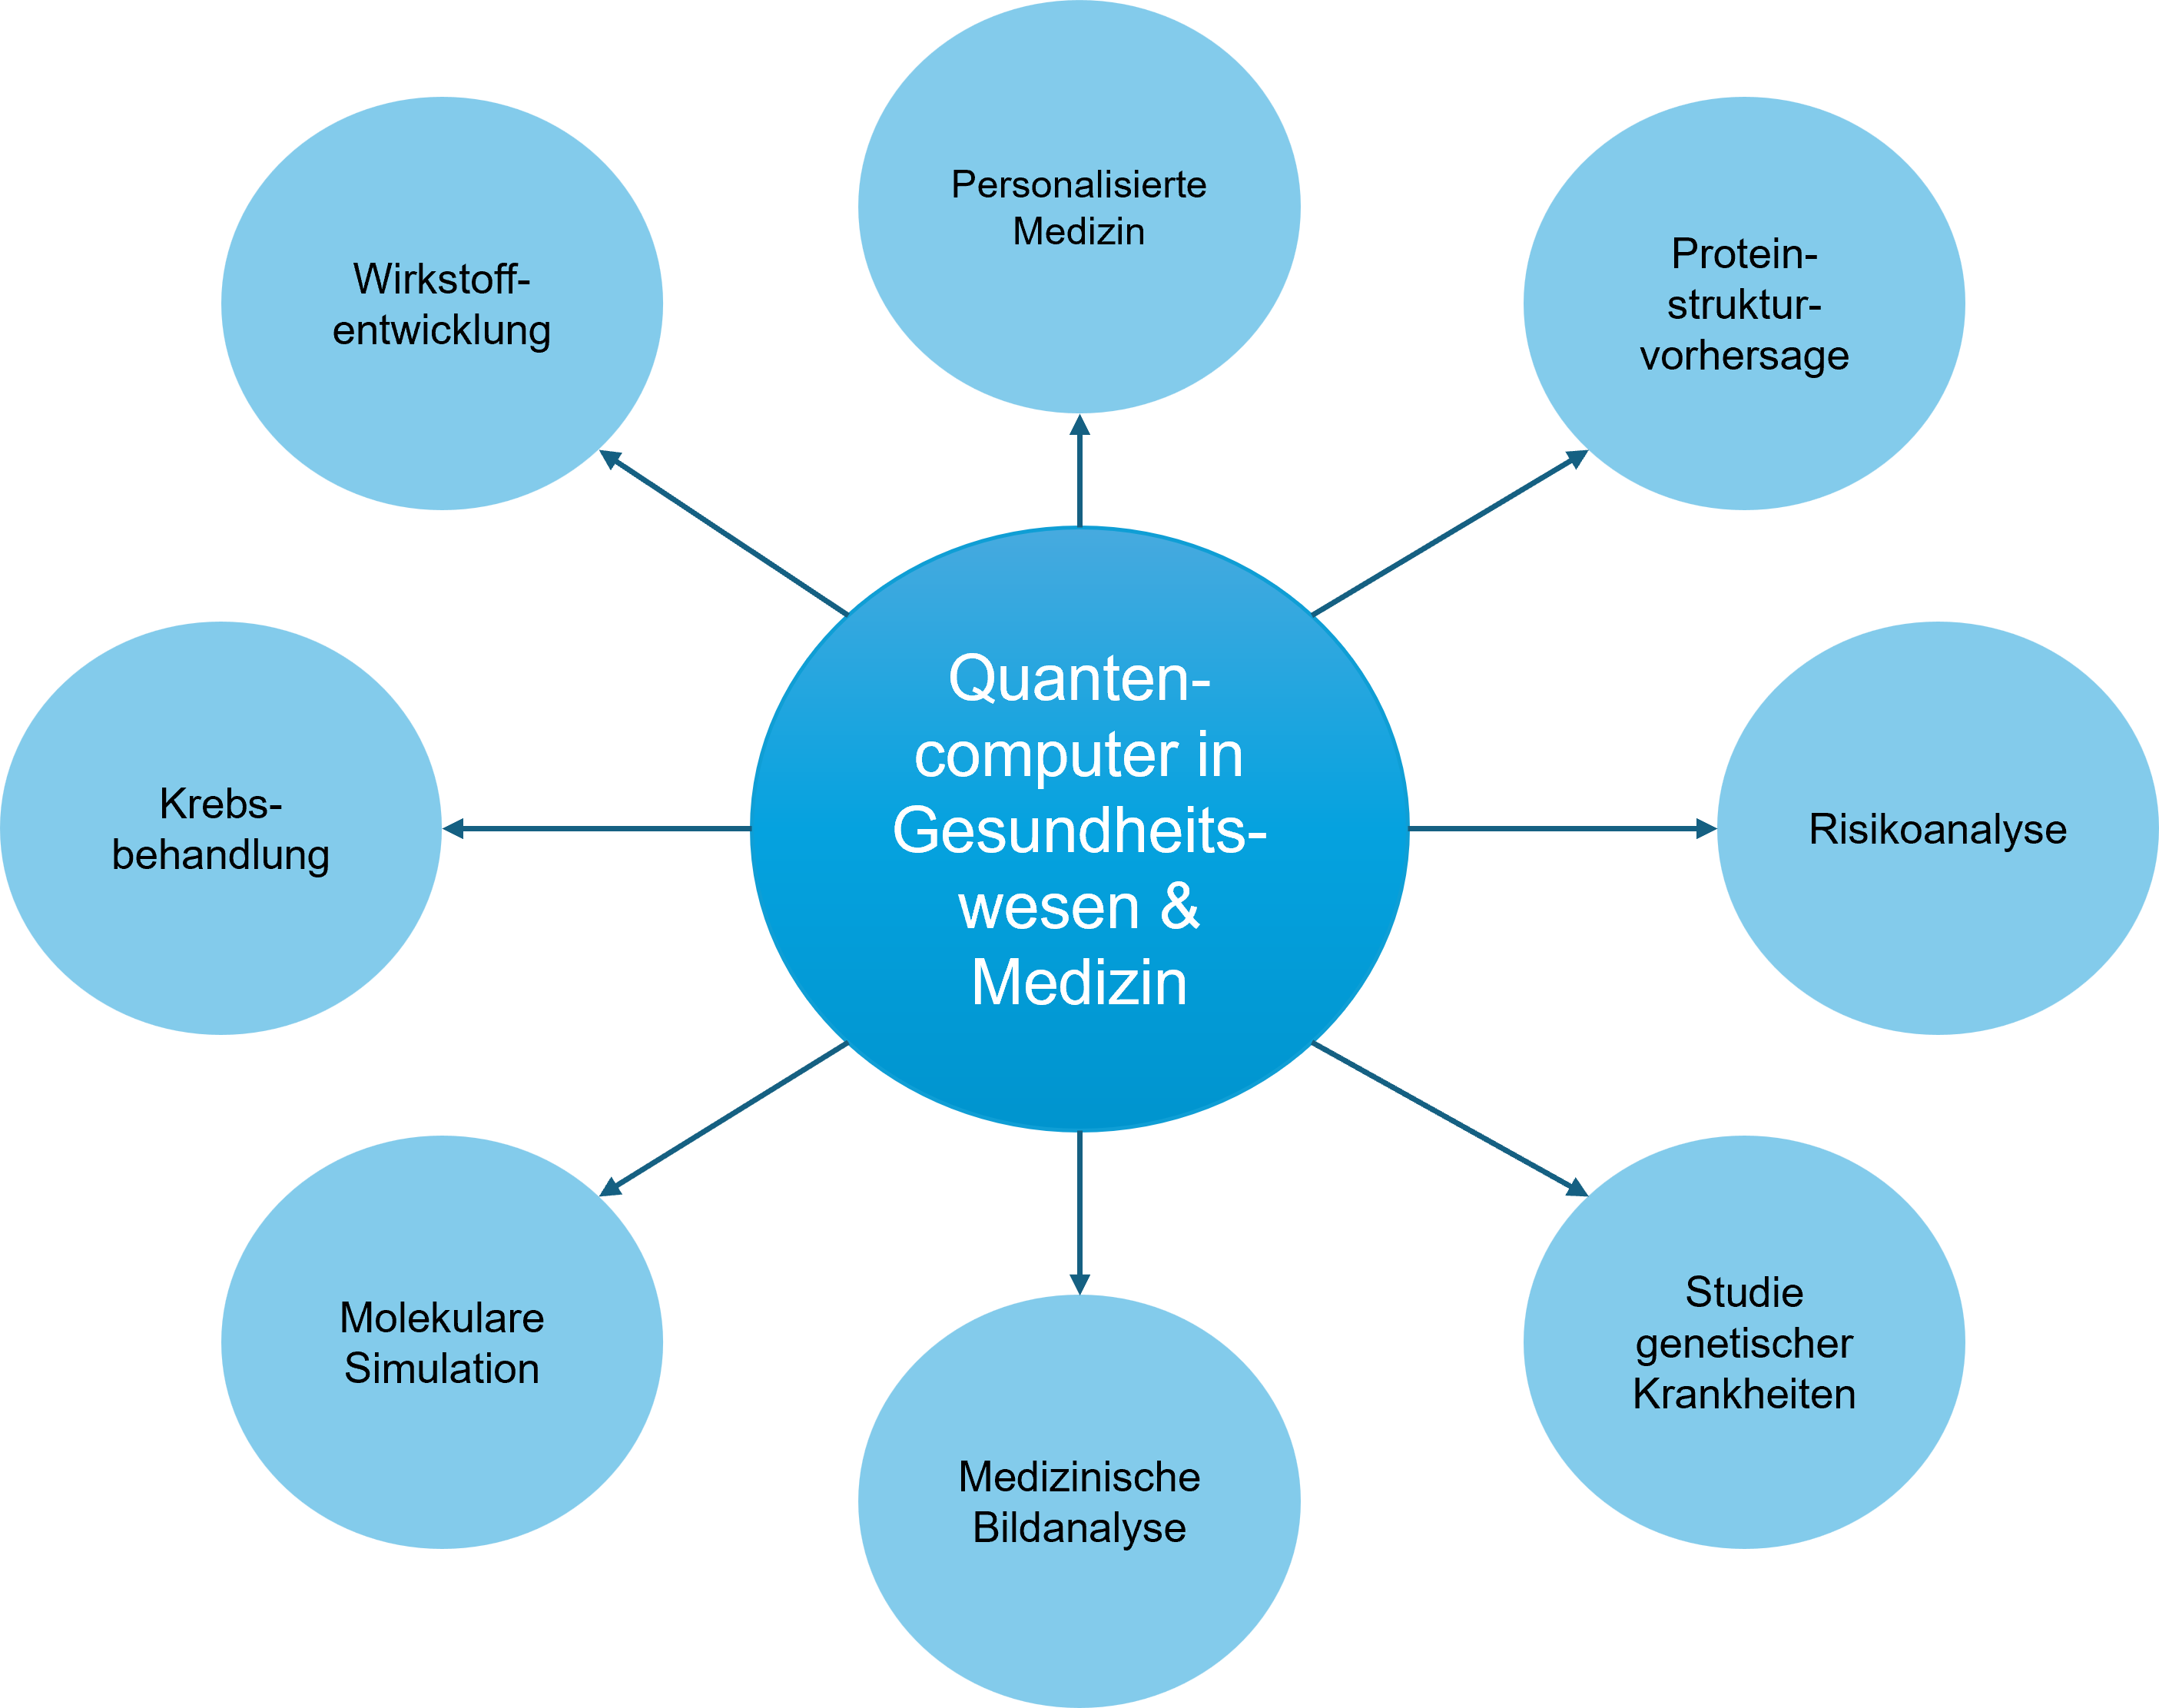
\includegraphics[width=.8\textwidth]{images/medicine/AnwendungsfelderMedizin.png}
    \caption{Übersicht möglicher Einsatzfelder von Quantencomputern in der Medizin. (Eigene Darstellung nach \cite{dhande_quantum_2023}.)}
    \label{fig:use-cases-medicine}
\end{figure}
\\
Diese Auswahl basiert auf drei qualitativen Kriterien: Erstens adressieren diese Bereiche relevante medizinische Herausforderungen. Zweitens zeichnen sie sich durch eine besonders hohe rechnerische Komplexität aus, die den Einsatz von Quantencomputern sinnvoll erscheinen lässt. Drittens bestehen bereits erste praxisnahe Anwendungen und Pilotprojekte, die eine Brücke zwischen theoretischem Potenzial und konkreter Nutzung bilden. Die Auswahl orientiert sich somit nicht nur an theoretischem Potenzial, sondern auch an praktischer Umsetzbarkeit und gesellschaftlicher Relevanz.

\subsection{Wirkstoffentwicklung}
Die Entwicklung neuer Wirkstoffe ist grundlegend mit hohen Kosten verbunden. Das liegt besonders an langen Entwicklungszyklen und einer geringen Erfolgsquote. Der Einsatz von Computern, besonders im Rahmen des Computer"=Aided Drug Design (CADD), ist in der pharmazeutischen Forschung etabliert. Dies stößt jedoch bei der Modellierung komplexer molekularer Systeme an seine Grenzen (Vgl. \cite{bertl_quantum_2025}).\\
\\
Ein wichtiger Einsatzbereich von Quantencomputern in der Wirkstoffentwicklung ist die präzise Berechnung molekularer Eigenschaften. Besonders relevant sind hier der Variational Quantum Eigensolver (VQE) und die Quantum Phase Estimation (QPE). Diese Algorithmen werden genutzt, um die Schrödinger-Gleichung für Moleküle zu lösen. Damit lassen sich elektronische Strukturen, Energiezustände oder Bindungseigenschaften genauer bestimmen. Das ist zentral, um zu verstehen, wie ein Wirkstoff mit seinem Ziel im Körper interagiert. Ergänzend dazu kommen weitere Methoden zum Einsatz. Quantum Machine Learning (QML) kann molekulare Eigenschaften auf Basis quantenmechanischer Daten vorhersagen oder helfen, Wirkstoffkandidaten gezielt zu verbessern. Quantum Annealing eignet sich gut für Optimierungsprobleme, zum Beispiel um stabile Molekülkonfigurationen mit starker Zielbindung zu finden. Auch Prozesse wie die Aufnahme, Verteilung und Wirkung eines Medikaments im Körper, also Pharmakokinetik und Pharmakodynamik, lassen sich mit Quantenmodellen realistischer simulieren. So kann Quantencomputing an verschiedenen Stellen der Wirkstoffentwicklung unterstützen. (Vgl. \cite{bertl_quantum_2025})

\subsubsection*{Compound Screening \& Lead"=Optimierung}
Quantencomputer versprechen, diese Prozesse durch genauere und schnellere Simulationen von Molekülen und deren Wechselwirkungen erheblich zu verbessern. Dabei konzentrieren sich aktuelle Quantencomputing"=Anwendungen in der pharmazeutischen Forschung besonders auf zwei frühe Phasen der Wirkstoffentwicklung: das \textit{Compound Screening} und die \textit{Lead"=Optimierung}. Beim Compound Screening werden sehr viele verschiedene chemische Verbindungen daraufhin untersucht, ob sie grundsätzlich an ein Zielmolekül (z.B. ein krankheitsrelevantes Protein) binden können. In der Lead"=Optimierung werden dann vielversprechende Kandidaten gezielt verbessert, um deren Wirksamkeit und Verträglichkeit zu steigern. Quantencomputer können in diesen Phasen helfen, indem sie Wechselwirkungen zwischen Molekülen genauer simulieren und energetisch günstige Strukturen besser vorhersagen (Vgl. \cite{zinner_quantum_2021}).

\subsubsection*{Quantenchemische Simulation}
Auf theoretischer Ebene gilt die quantenchemische Berechnung von Molekül"=Energien als eines der vielversprechendsten Anwendungsfelder des Quantencomputings. Sie ist essenziell für die Ermittlung von Bindungsaffinitäten, Reaktionspfaden und energetisch bevorzugten Konformationen, welche zentrale Größen in der computergestützten Wirkstoffentwicklung sind. Wie \cite{cao_quantum_2019} betonen: Das klassische Problem, dessen Lösung vom Quantencomputing erwartet wird, ist die Berechnung von Grundzustands- und angeregten Zustandsenergien kleiner Moleküle. Solche Berechnungen dienen als Ausgangspunkt für die Bestimmung vieler nützlicher Größen, wie etwa Reaktionspfaden, Bindungsenergien und Reaktionsgeschwindigkeiten chemischer Prozesse. (eigene Übersetzung nach \cite{cao_quantum_2019}.) Zentral ist demnach die Berechnung von Molekülenergien, da sie viele wichtige chemische Eigenschaften bestimmt.

\subsubsection*{Virtuelles Screening und datengetriebene Modellierung}
Beim \textit{virtuellen Screening} handelt es sich um einen frühen Schritt im Prozess der Wirkstoffentwicklung. Dabei werden mit Hilfe von Computern große Datenbanken nach Molekülen durchsucht, die an ein bestimmtes krankheitsrelevantes Ziel binden könnten. So lassen sich vielversprechende Wirkstoffkandidaten schneller finden und unnötige Labortests vermeiden. Klassische Methoden stoßen dabei aber oft an Grenzen: Die Modelle sind manchmal ungenau, liefern viele falsche Treffer und brauchen viel Rechenleistung. Neue Ansätze wie Quantum Machine Learning können hier helfen. Mit Quantencomputern lassen sich Molekülwechselwirkungen genauer simulieren und komplexe Daten effizienter verarbeiten. Techniken wie Quanten"=Neuronale Netzwerke, Quanten"=Kernel oder spezielle Quanten"=Suchalgorithmen ermöglichen ein gezielteres und schnelleres Screening. (Vgl. \cite{kumar_recent_2024})


\subsection{Proteinstrukturvorhersage}
\label{med:protein}
Die bisher etablierten Methoden zur Proteinstrukturvorhersage haben bereits beeindruckende Fortschritte erzielt. Mit experimentellen Ansätzen sowie durch KI"=basierte Modelle wie AlphaFold, RoseTTaFold und verwandte Systeme lassen sich für viele Proteine dreidimensionale Strukturen bereits mit hoher Genauigkeit vorhersagen. (Vgl. \cite{jumperHighlyAccurateProtein2021}; \cite{baekAccuratePredictionProtein2021})\\
\\
Besonders relevant ist dabei der VQE, der in hybriden Verfahren genutzt wird, um energiearme Faltungskonfigurationen zu berechnen. Auch quantumbasierte Optimierungsansätze auf Gittermodellen spielen eine Rolle, da sie es erlauben, Faltungsprozesse vereinfacht, aber physikalisch fundiert zu simulieren. Diese Algorithmen bieten eine Alternative zu klassischen Methoden, die bei komplexen oder künstlichen Proteinsequenzen oft an ihre Grenzen stoßen. (Vgl. \cite{doga_perspective_2024}; \cite{robert_resource-efficient_2021})

\subsubsection*{Grenzen klassischer Methoden}
Diese klassischen Methoden basieren meist auf Mustern aus bekannten Proteinstrukturen und liefern häufig nur ein begrenztes Verständnis der physikalischen Prozesse, die der Proteinfaltung zugrunde liegen. Das erschwert insbesondere die Vorhersage bei synthetischen oder stark abweichenden Aminosäuresequenzen. Studien zeigen, dass Modelle wie AlphaFold2 bei solchen Sequenzen außerhalb ihres Trainingsdatensatzes unzuverlässige Ergebnisse liefern können (Vgl. \cite{outeiralCurrentStructurePredictors2022}). Physikbasierte Verfahren wie die Molekulardynamik bieten zwar grundsätzlich eine höhere Genauigkeit, sind jedoch für größere Proteine extrem rechenintensiv und in der Praxis kaum skalierbar (Vgl. \cite{doga_perspective_2024}). Diese Einschränkungen verdeutlichen den Bedarf an alternativen Modellierungsansätzen.

\subsubsection*{Quantenbasierte Faltungsmodelle}
Quantencomputer könnten eine vielversprechende Alternative bieten, da sie durch Quantenparallelismus potenziell viele Faltungszustände gleichzeitig analysieren können (Vgl. \cite{doga_perspective_2024}). Aktuelle Forschungsarbeiten formulieren die Proteinfaltung dabei als Optimierungsproblem und setzen auf Quantenalgorithmen sowie vereinfachte physikalische Modelle. Zwei Ansätze haben sich dabei als besonders vielversprechend erwiesen: Hybridverfahren mit VQE und quantenbasierte Gittermodelle.\\
\\
Im Ansatz von \citeauthor{doga_perspective_2024} wurde ein hybrider Algorithmus eingesetzt, der klassische Optimierung mit einem VQE kombiniert. Ziel war die Vorhersage der Struktur eines kurzen Abschnitts mit sieben Aminosäuren aus dem Helikaseprotein des Zika"=Virus. Solche Abschnitte werden als Loops bezeichnet. Sie verbinden regelmäßige Strukturelemente wie Alpha"=Helices und Beta"=Faltblätter und sind häufig entscheidend für die Funktion eines Proteins. Die räumliche Anordnung der Atome in diesem Abschnitt, also die sogenannte Konformation, wurde anschließend mit bekannten Referenzdaten verglichen. Die mittels Quantencomputer berechnete Struktur wich deutlich weniger vom experimentell bestimmten Referenzmodell ab als die Vorhersage von AlphaFold2. Der mittlere Abstand der Atome (RMSD) betrug etwa 1,88 Å bei der Quantenmethode und 3,53 Å bei AlphaFold2. Das zeigt, dass quantenbasierte Verfahren bereits heute genauere Ergebnisse liefern können als etablierte KI"=Modelle. Zumindest für kleinere, aber strukturell anspruchsvolle Proteinbereiche. (Vgl. \cite{doga_perspective_2024})\\
\\
Ein weiterer Ansatz basiert auf Gittermodellen. \citeauthor{robert_resource-efficient_2021} verwendeten ein solches Modell zur Faltung kurzer Peptide mit IBM-Quantenhardware. Ein 10"=Aminosäure"=Peptid (Angiotensin) wurde auf 22 Qubits, ein 7-Aminosäure-Peptid auf 9 Qubits kodiert. Die Ergebnisse zeigen, dass selbst kleine Quantencomputer bereits in der Lage sind, realistische Faltungskonfigurationen effizient zu berechnen. (Vgl. \cite{robert_resource-efficient_2021})


\subsection{Personalisierte Medizin}
Die personalisierte Medizin verfolgt das Ziel, medizinische Entscheidungen stärker an den individuellen Eigenschaften eines Patienten auszurichten, etwa an genetischen Merkmalen, Krankheitsverläufen oder Therapieansprechen. Das bedeutet, dass aus komplexen, oft hochdimensionalen Daten wie Genomsequenzen, Laborwerten oder Bilddaten präzise Vorhersagen abzuleiten sind. Klassische Methoden stoßen hierbei zunehmend an ihre Grenzen, insbesondere bei kleinen Datensätzen, hoher Variabilität oder stark nichtlinearen Zusammenhängen. Auch maschinelles Lernen stoßt bei individuellen oder seltenen Fällen oft an seine Grenzen. Bei wenigen Trainingsdaten führen sie zu unsicheren Diagnosen und Therapieentscheidungen. (Vgl. \cite{gupta_systematic_2025}).\\
\\
Einige Algorithmen spielen in der personalisierten Medizin eine besonders wichtige Rolle. QML und QNN eignen sich, um individuelle Krankheitsverläufe und Therapieantworten vorherzusagen. Erste Studien zeigen, dass sich damit zum Beispiel Tumordynamiken modellieren oder Therapieergebnisse besser abschätzen lassen. Ergänzend werden QAOA und VQA eingesetzt, etwa zur Planung klinischer Studien oder zur Auswahl geeigneter Patientengruppen. Auch generative Modelle wie Quantum Boltzmann Machines finden Anwendung, etwa zur Erzeugung synthetischer Patientendaten. Diese Methoden erweitern die Möglichkeiten klassischer Verfahren, ohne sie vollständig zu ersetzen. (Vgl. \cite{bertl_quantum_2025})

\subsubsection*{P5"=Medizin}
In der aktuellen Forschung wird personalisierte Medizin zunehmend als sogenanntes P5"=Modell verstanden. Dieses erweitert das bisherige P4"=Modell um eine fünfte Dimension: \textit{psychokognitiv}. Die fünf Elemente lauten: vorhersagend (predictive), vorbeugend (preventive), personalisiert, beteiligend (participatory) und psychokognitiv. Letztere betont psychologische und kognitive Faktoren wie Werte, Lebensqualität und Gesundheitskompetenz. Diese beeinflussen, wie Patienten mit Erkrankungen umgehen und wie sie auf Therapien reagieren. (Vgl. \cite{gorini_p5_2011})\\
\\
Quantencomputing kann in diesem Kontext neue Wege eröffnen. Durch seine Fähigkeit, viele Datenmuster gleichzeitig zu analysieren, lassen sich verhaltensbezogene Einflussfaktoren stärker in personalisierte Modelle integrieren. Besonders vielversprechend ist hier der Einsatz von Quantum Machine Learning, also von Modellen, die klassische Lernverfahren mit quantenmechanischen Elementen kombinieren (Vgl. \cite{bertl_quantum_2025}.)

\subsubsection*{Frühe Anwendungen von Quantum Machine Learning}
Eine aktuelle Übersichtsarbeit zeigt, dass sich erste klinisch relevante QML-Anwendungen zum Beispiel in der EKG"=Analyse, Genomik oder Bildgebung bereits auf echter Quantenhardware testen lassen, wenn auch bisher in begrenztem Umfang (Vgl. \cite{gupta_systematic_2025}). Besonders Genomik und Bildgebung ermöglichen eine präzisere Diagnostik und auf individuelle genetische Profile abgestimmte Therapieansätze. Ein konkretes Beispiel liefert eine Studie zur Vorhersage von Arzneimittelwirkungen bei Krebspatienten. In dieser erzielt ein hybrides QNN eine bis zu 15 Prozent höhere Genauigkeit als klassische Modelle, bei signifikant kürzerer Trainingszeit (Vgl. \cite{sagingalieva_hybrid_2023}).\\
\\
\begin{table}[ht]
\centering
\renewcommand{\arraystretch}{1.3}
\resizebox{\textwidth}{!}{
\begin{tabular}{|p{2.3cm}|p{4.5cm}|p{2.5cm}|p{4.5cm}|}
\hline
\textbf{Anwendungsfeld} & \textbf{Rechnerische Herausforderung} & \textbf{Quantenansatz / Algorithmus} & \textbf{Warum QC relevant?} \\
\hline
Drug Discovery & Molekül-Energieberechnung, Bindungsaffinitäten & VQE, QPE & Klassische Methoden zu ungenau oder zu langsam \\
\hline
Proteinstruktur & Kombinatorische Explosion möglicher Faltungen & QAOA, Hybridalgorithmen & QC kann Zustände simultan analysieren \\
\hline
Personalisierte Medizin & Mustererkennung in hochdimensionalen Daten & QML, QNN & Klassische Modelle überfordert bei komplexer Nichtlinearität \\
\hline
\end{tabular}
}
\caption{Anwendungsfelder des Quantencomputings in der Medizin und Pharmazie}
\label{tab:qc_medizin}
\end{table}
\\


\section{Top Technologien \& Algorithmen}

\subsection{Variational Quantum Eigensolver (VQE)}
Der Variational Quantum Eigensolver (VQE) ist ein Algorithmus zur Lösung quantenchemischer Probleme und findet zunehmend Anwendung im medizinischen Kontext. In der quantenchemischen Simulation kann VQE genutzt werden, um Molekülenergien, Bindungsaffinitäten und Reaktionspfade zu berechnen. Diese Größen sind entscheidend für die Beurteilung chemischer Stabilität und Reaktivität und spielen eine wichtige Rolle bei der frühen Identifikation potenzieller Wirkstoffe (Vgl. \cite{palFuturePotentialQuantum2024}; \cite{cao_quantum_2019}). Darüber hinaus wird VQE auch in der Strukturbiologie erforscht. Er kann eingesetzt werden, um die Energie von Proteinbausteinen oder Ligand-Protein-Komplexen abzuschätzen, was dazu beiträgt, molekulare Wechselwirkungen besser zu verstehen (\cite{marchettiQuantumComputingAlgorithms2022}). Studien deuten zudem darauf hin, dass VQE künftig auch für die Simulation individueller Stoffwechselprozesse genutzt werden könnte. Dies betrifft beispielsweise Anwendungen in der personalisierten Medizin, etwa zur Vorhersage individueller Therapieerfolge oder bei der Entwicklung neuer Kontrastmittel für bildgebende Verfahren (\cite{palFuturePotentialQuantum2024}).

\subsection{Quantum Phase Estimation (QPE)}
Der Quantum Phase Estimation (QPE) Algorithmus gilt als zentrale Methode zur präzisen Bestimmung von Grundzustandsenergien von Molekülen und ist damit von besonderem Interesse für die Wirkstoffentwicklung, etwa bei pharmazeutisch relevanten Substanzen wie Ibrutinib. Im Vergleich zu klassischen Verfahren bietet QPE das Potenzial für eine exponentielle Beschleunigung solcher Berechnungen. Die herkömmliche Lehrbuchvariante von QPE ist jedoch sehr ressourcenintensiv und anfällig für Fehler, da sie zahlreiche Hilfs-Qubits und tiefe Schaltkreise erfordert. Um diese Limitierungen zu überwinden, wurden speziell für frühe fehlertolerante Quantencomputer (EFTQCs) optimierte Protokolle wie Iterative Phase Estimation (IPE), Robust Phase Estimation (RPE), Quantum Complex Exponential Least Squares (QCELS) und Multi"=Modal Multi"=Level QCELS (MMQCELS) entwickelt. Diese reduzieren sowohl die Zahl der benötigten Ancilla"=Qubits als auch die Schaltungstiefe und verbessern die Robustheit gegenüber Fehlern deutlich. Studien zeigen, dass das Berechnungsvolumen im Vergleich zur klassischen QPE um ein Vielfaches gesenkt werden kann. Teilweise um das bis zu 300-Fache. Ergänzend leisten Fortschritte in der Optimierung der Simulationstechniken und der Fehlerminderung einen Beitrag zur praktischen Umsetzbarkeit dieser Methoden. (Vgl. \cite{nelson_assessment_2024}; \cite{blunt_perspective_2022}; \cite{blunt_statistical_2023})

\subsection{Quantum Approximate Optimization Algorithm (QAOA)}
QAOA ist ein variationaler Quantenalgorithmus zur näherungsweisen Lösung kombinatorischer Optimierungsprobleme, der im medizinischen Bereich insbesondere in der Proteinfaltung und im molekularen Docking Anwendung findet. Für das Proteinfaltungsproblem wurde QAOA in vereinfachten Gittermodellen getestet, wobei es energiearme Konformationen mit höherer Wahrscheinlichkeit erzeugen konnte als rein zufälliges Sampling. Allerdings erfordern realistischere Modelle deutlich tiefere Quantenschaltkreise, was eine Anwendung auf atomarer Ebene derzeit noch erschwert. Größeres Potenzial zeigt QAOA im Bereich des molekularen Dockings, das für die Entwicklung neuer Medikamente zentral ist. Durch die Formulierung des Problems als maximal gewichtete Clique lassen sich mit dem verbesserten DC"=QAOA"=Ansatz biologisch relevante Bindungsstellen effizienter identifizieren. Fallstudien mit relevanten Zielproteinen wie SARS"=CoV"=2 Mpro, DPP-4 und HIV-1 gp120 belegen eine hohe Übereinstimmung mit bekannten Strukturen. Gleichzeitig zeigt DC"=QAOA Vorteile bei der Ressourcennutzung, da es weniger Gatter und Iterationen benötigt als klassische Varianten. Herausforderungen bestehen weiterhin in der Stabilität der Optimierung, insbesondere bei komplexeren molekularen Systemen. (Vgl. \cite{ding_molecular_2024}; \cite{boulebnane_peptide_2023})

\subsection{Hybride Quantenklassische Algorithmen}
Hybride quantenklassische Algorithmen kombinieren klassische Rechenmethoden mit quantenmechanischen Komponenten und gelten als vielversprechender Ansatz für medizinische Anwendungen im Zeitalter begrenzter Quantenhardware. Besonders in der personalisierten Medizin und Wirkstoffentwicklung zeigen sich erste sinnvolle Einsatzmöglichkeiten. So lassen sich etwa Biomarker für bestimmte Krebsarten wie das klarzellige Nierenzellkarzinom genauer klassifizieren, was die Diagnose verbessern und Therapien gezielter ermöglichen kann. Auch in der computergestützten Entwicklung neuer Medikamente bieten hybride Verfahren Vorteile, zum Beispiel bei der Simulation chemischer Bindungen oder der Bewertung pharmakologisch relevanter Energieprofile. Diese Ansätze verdeutlichen, dass sich Quantencomputing bereits heute sinnvoll mit bestehenden Methoden verknüpfen lässt, um medizinische Entscheidungsprozesse zu unterstützen. (Vgl. \cite{li_hybrid_2024}; \cite{astuti_use_2025})

\subsection{Quantum Machine Learning (QML) \& Quantum Neural Networks (QNN)}
Quanten-Maschinelles Lernen (QML) und Quanten-Neuronale Netzwerke (QNN) sind speziell entwickelte Quantenalgorithmen zur Analyse klassischer Gesundheitsdaten. Insbesondere im Zuge der zunehmenden Digitalisierung, etwa durch elektronische Gesundheitsakten, gelten sie als vielversprechende Werkzeuge für klinische Entscheidungshilfen, Gesundheitsprognosen und kontinuierliches Monitoring. QNNs kommen dabei als gate-basierte Modelle zum Einsatz, die sich gezielt für solche Aufgaben einsetzen lassen. Eine systematische Übersichtsarbeit zu Veröffentlichungen zwischen 2015 und 2024 zeigt jedoch, dass es bislang an empirischer Evidenz für einen klaren Vorteil gegenüber klassischen Verfahren mangelt. Die meisten Studien konzentrierten sich auf Diagnose- und Prognoseanwendungen, während wichtige Bereiche wie Public Health oder Versorgungsforschung kaum berücksichtigt wurden. Darüber hinaus erfolgten viele Untersuchungen unter idealisierten Bedingungen und setzten vereinfachte, lineare Modelle ein, ohne reale Fehlerquellen zu integrieren. (Vgl. \cite{gupta_systematic_2025})

\subsection{Technologische Frameworks}
Die in diesem Abschnitt vorgestellten technologischen Frameworks orientieren sich an den in Kapitel \ref{med:applicationFields} beschriebenen Anwendungsfeldern. Ziel ist es, die eingesetzten Softwarestacks und Entwicklungstools entlang ihrer praktischen Einsatzbereiche in der Wirkstoffentwicklung, der Proteinstrukturvorhersage und der personalisierten Medizin systematisch darzustellen. Auf diese Weise wird deutlich, wie spezifische Quantenalgorithmen in den jeweiligen medizinischen Kontexten technologisch implementiert werden.\\

\subsubsection*{Wirkstoffentwicklung}
Die praktische Umsetzung der Quantenalgorithmen für medizinische Anwendungen erfordert leistungsfähige Software"=Stacks, die Quanten-Hardware und klassische Algorithmen verbinden. Für die Wirkstoffentwicklung werden vor allem Frameworks genutzt, die komplexe \textit{Molekül"=Hamilton"=Operatoren} bearbeiten und Verfahren wie VQE oder QPE effizient implementieren. Bei den Operatoren handelt es sich um mathematische Ausdrücke, die alle relevanten physikalischen Eigenschaften eines Moleküls quantenmechanisch beschreiben. Der Hamilton"=Operator bildet somit die Grundlage für die Simulation von Molekülzuständen, da er die Energieverteilung eines Systems vollständig bestimmt (Vgl. \cite{mcardle_quantum_2020}).\\
\\
So bietet IBM Qiskit mit dem Qiskit Nature"=Modul spezialisierte Werkzeuge zur Darstellung chemischer Systeme und zum Lösen von Grundzustandsproblemen in Molekülen (Vgl. \cite{developers_qiskit_2023}). Microsofts Q\# Quantum Development Kit (QDK) enthält ebenfalls eine Chemie-Bibliothek mit qubitisierten Fermionen-Operatoren sowie Implementierungen von Hamilton-Simulatoren (Trotterisierung, Qubitierung) (Vgl. \cite{team_simulating_2018}). \\
\\
Amazon Braket ist ein vollständig verwalteter Cloud-Dienst von AWS, der es Forscherinnen und Forschern ermöglicht, Quantenalgorithmen zu entwerfen, auf verschiedenen Simulatoren zu testen und auf realen Quantencomputern auszuführen. Damit bietet Braket eine flexible Entwicklungsumgebung für hybride quantenklassische Workflows in der Arzneimittelforschung. Besonders relevant für medizinische Anwendungen ist der Zugriff auf unterschiedliche Hardwareplattformen innerhalb eines einheitlichen SDK. Braket unterstützt unter anderem gatterbasierte Quantencomputer von IonQ, IQM und Rigetti sowie einen Analog Hamiltonian Simulator (AHS) von QuEra. Letzterer erlaubt die direkte Simulation physikalischer Systeme auf Basis kontinuierlicher Hamilton-Operatoren, was für bestimmte molekulare Strukturberechnungen von Vorteil sein kann (Vgl. \cite{noauthor_quantum_nodate-1}). Dieser flexible Ansatz wird beispielsweise im AWS"=Toolkit QCEDD genutzt, das eingebaute Beispiele für Aufgaben wie molekulares Docking und Faltungsprobleme in der Wirkstoffforschung enthält. (Vgl. \cite{noauthor_quantum_nodate})\\ %evtl. git repo zitieren

%besonders beim virtuellen screening relevant 

\subsubsection*{Proteinstrukturvorhersage}
Die Vorhersage von Proteinstrukturen ist ein hochdimensionales Optimierungsproblem. Klassischerweise modelliert man Proteine auf Gitternetzen, um die Konformationsräume lösbar zu machen. Wie bereits in Kapitel \ref{med:protein} dargelegt, sind Quantenoptimierungsalgorithmen wie QAOA dafür gut geeignet. (Vgl. \cite{boulebnane_peptide_2023})\\
\\
Zur praktischen Umsetzung von Algorithmen wie QAOA in der Proteinstrukturvorhersage wird geeignete Software benötigt, die die Komplexität quantenmechanischer Optimierung handhabbar macht. Ein bekanntes Framework in diesem Bereich ist \textit{PennyLane}. Es ist eine plattformunabhängige Open"=Source"=Bibliothek für Quantencomputing und Quantum Machine Learning, die für wissenschaftliche Anwendungen entwickelt wurde. Durch PennyLane können Quantenalgorithmen mit klassischen Lernverfahren kombiniert werden. Das ist besonders bei der Proteinstrukturvorhersage von Vorteil, da hier sowohl quantenbasierte Optimierung, als auch klassische Auswertungsverfahren erforderlich sind. (Vgl. \cite{noauthor_what_nodate})\\
\\
Das Start"=up Menten AI nutzt PennyLane für die Entwicklung neuer proteinbasierter Wirkstoffe. Ziel ist es, Quantencomputing und klassische Verfahren so zu kombinieren, dass neue Wirkstoffkandidaten schneller und gezielter gefunden werden können. Dabei setzt Menten AI auf PennyLane, um Quantenalgorithmen effizient einzubinden und bioaktive Peptide für neue Therapien zu entwickeln. Das heißt, sie nutzen die Software, um schneller passende Wirkstoffe zu finden, die gut an bestimmte Krankheitsziele andocken können. (Vgl. \cite{abdel-kareemXanaduUSAir2025})\\

\subsubsection*{Personalisierte Medizin}
In der personalisierten Medizin stehen große und komplexe Datensätze im Fokus, zum Beispiel aus Genomik, Bildgebung oder klinischen Untersuchungen. Um diese besser auszuwerten, werden zunehmend Frameworks genutzt, die klassische Machine"=Learning"=Modelle mit Quantenkomponenten verbinden. Ein wichtiges Beispiel ist \textit{TensorFlow Quantum}, das das Quantenframework \textit{Cirq} mit dem bekannten Lernframework \textit{TensorFlow} kombiniert. Es ermöglicht hybride Modelle, bei denen klassische und quantenbasierte Rechenschritte gemeinsam genutzt werden. Das ist besonders relevant, da Quantenprozessoren aktuell noch fehleranfällig und begrenzt einsetzbar sind. Durch die Kombination mit klassischen Prozessoren kann das Potenzial von Quantenalgorithmen gezielter genutzt werden. TensorFlow Quantum erlaubt es, Quantenschaltungen direkt in neuronale Netze einzubinden und diese automatisch zu trainieren. Ein weiterer Vorteil liegt im Umgang mit sogenannten Quantendaten, etwa aus Quantenchemiesimulationen oder hochpräzisen Messungen, die für neue Medikamente oder Diagnoseverfahren genutzt werden können. Mit dem Simulator \textit{qsim} steht zudem eine leistungsfähige Entwicklungsumgebung zur Verfügung. Das Framework bietet also neue Möglichkeiten, komplexe medizinische Daten zu analysieren und Muster zu erkennen, die für personalisierte Behandlungsentscheidungen wichtig sind. (Vgl. \cite{broughton_tensorflow_2021})

\section{Wichtige Unternehmen \& Akteure}

\subsection{Allgemeiner Überblick}
Mit dem wachsenden Interesse an der Nutzung von Quantencomputing zur Lösung komplexer Probleme in der Medizin und Pharmazie rücken weltweit Technologieunternehmen, Start-ups sowie akademische Institutionen zunehmend in den Fokus.\\

IBM Quantum zählt zu den führenden Unternehmen im Bereich der Quantenmedizin. Seit der Einführung des ersten cloudbasierten Quantencomputers (2016), des Open-Source-Frameworks Qiskit (2017) und des IBM Quantum System One (2019) verfolgt IBM eine klare Strategie zur Kommerzialisierung und Skalierung quantentechnologischer Anwendungen. Die 2020 veröffentlichte Entwicklungs-Roadmap unterstreicht den langfristigen Fokus auf Quantencomputing mit gatterbasierten Architekturen und integrierter Fehlerkorrektur, die sich besonders für präzise quantenchemische Simulationen eignen. (Vgl. \cite{abughanemIBMQuantumComputers2025},\cite{jaygambettaIBMRoadmapQuantumcentric2022}, \cite{bravyiHighthresholdLowoverheadFaulttolerant2024}, \cite{mullerImprovedBeliefPropagation2025}) Im Rahmen des IBM Quantum Netzwerks bestehen über 250 Kooperationen mit führenden Forschungseinrichtungen und Unternehmen, darunter Moderna, die Cleveland Clinic, Bosch sowie mehrere Universitäten wie Chicago und Heidelberg. (Vgl. \cite{noauthor_ibm_nodate})\\

Auch Google treibt unter dem Dach von Google Quantum AI die Entwicklung quantentechnologischer Anwendungen voran – insbesondere in Kombination mit künstlicher Intelligenz und durch Kooperation mit DeepMind. In Zusammenarbeit mit internationalen Partnern wie der Universität Luxemburg und dem Max-Planck-Institut werden neuartige Methoden zur Simulation biomolekularer Dynamik erforscht. (Vgl. \cite{unkeBiomolecularDynamicsMachinelearned2024}) Mit dem 54-Qubit-Chip Sycamore demonstrierte Google bereits 2019 die sogenannte Quantum Supremacy. 2024 folgte mit dem 105-Qubit-Prozessor Willow ein weiterer technologischer Meilenstein, insbesondere im Bereich der Fehlerkorrektur. (Vgl. \cite{arute_quantum_2019, acharya_quantum_2025}) Google arbeitet zudem seit 2021 mit Boehringer Ingelheim und seit 2023 mit Bayer zusammen, um Quantentechnologie zur Beschleunigung pharmazeutischer Anwendungen wie Wirkstoffscreening und genomischer Analyse einzusetzen. (Vgl. \cite{ingelheimCooperationGoogleQuantum2021, BayerAccelerateDrug})\\

Microsoft verfolgt mit der Plattform Azure Quantum einen ganzheitlichen Ansatz, der Hochleistungsrechnen, KI und Quantenprozessoren vereint – auch im medizinisch-pharmazeutischen Bereich. Die Lösung Azure Quantum Elements nutzt multimodale KI-Modelle und großskalige biologische Daten zur Beschleunigung quantenchemischer Simulationen. (Vgl. \cite{buntzMicrosoftEyesQuantum2023}) Zentraler Bestandteil von Microsofts Hardwareentwicklung ist der Majorana-Chip, der auf topologischen Qubits basiert und eine erhöhte Fehlertoleranz verspricht. (Vgl. \cite{aasenRoadmapFaultTolerant2025}, \cite{aghaeeInterferometricSingleshotParity2025}) Ein technischer Durchbruch gelang 2024 in Kooperation mit Quantinuum: die Skalierung und stabile Verschränkung von 12 logischen Qubits bei einer Gate-Fidelität von 99,8\%. Dieser Wert liegt nahe der praktischen Fehlertoleranzschwelle von 99,9\%. (Vgl. \cite{reichardtDemonstrationQuantumComputation2024})\\

D-Wave Systems gilt als einer der frühesten kommerziellen Anbieter quantentechnologischer Systeme – insbesondere im Bereich des Quantum Annealing. (Vgl. \cite{flahertyDWaveLooksLarge2024}) Gemeinsam mit Forschungseinrichtungen wie der University of British Columbia, der Jagiellonen-Universität und dem Max-Planck-Institut konnte 2024 eine experimentelle Quantenüberlegenheit bei realistischen Simulationen nachgewiesen werden. Die quantenbasierten Verfahren übertrafen dabei klassische Modelle wie Tensor-Netzwerke und neuronale Quantenzustandsalgorithmen signifikant. (Vgl. \cite{kingComputationalSupremacyQuantum2024})\\

Das Deeptech-Unternehmen Qubit Pharmaceuticals mit Verbindung zur Sorbonne University fokussiert sich auf hochaufgelöste molekulare Modellierung. Mithilfe quantenbasierter KI-Modelle sollen biophysikalische Systeme wie Proteinstrukturen, Ligandenbindung oder Hydratationsprozesse hochpräzise simuliert werden – ein zentraler Beitrag zur Wirkstoffforschung. (Vgl. \cite{gouraud_velocity_2025})\\

Auch führende Universitäten und Forschungsinstitute tragen maßgeblich zur Weiterentwicklung quantenmedizinischer Anwendungen bei. Sie kombinieren Quantenphysik, Chemie, Biomedizin und Informatik mit dem Ziel, diagnostische und therapeutische Verfahren zu revolutionieren. Die Universität Heidelberg gehört zu den Vorreitern im Bereich des Quantum Healthcare, mit Fokus auf quantengestützte Diagnostik, quantenchemische Simulationen und KI-gestützte Molekülanalysen. (Vgl. \cite{noauthor_hgsfp_nodate}) Die Harvard University zeichnet sich durch ihre exzellente Forschungsinfrastruktur aus und ist führend in der Entwicklung effizienter Quantenalgorithmen für die NMR-Spektroskopie sowie biophysikalischer Simulationen. Jüngste Arbeiten zeigen u.a. die technische Realisierbarkeit eines molekularen iSWAP-Gates mit ultrakalten polaren Molekülen – ein vielversprechender Baustein für universelle Quantenrechner in der medizinisch-pharmazeutischen Simulation. (Vgl. \cite{siliezar_harvard_2020, picard_entanglement_2025}) Die University of Tokyo zählt zu den zentralen asiatischen Forschungsstandorten im Bereich der Quantenpharmakologie. In Kooperation mit IBM wurde dort ein IBM Quantum System One installiert, das zur Simulation chemischer Prozesse im medizinischen Kontext dient. (Vgl. \cite{noauthor_utokyo_nodate})\\

Bereits heute existieren zahlreiche Pilotprojekte, Kooperationen und Proof-of-Concept-Studien, die das Potenzial von Quantencomputing in der Medizin- und Pharmaforschung demonstrieren. Ein herausragendes Beispiel im deutschsprachigen Raum ist die QuantumBW-Initiative in Baden-Württemberg, die zahlreiche Akteure aus Wissenschaft, Wirtschaft und Industrie vereint. Ziel dieser landesweiten Zusammenarbeit ist es, die vorhandene Expertise zu bündeln und Baden-Württemberg als führenden Standort für Quantenforschung und -anwendung zu etablieren. Beteiligt sind unter anderem die Städte Heidelberg, Karlsruhe, Stuttgart, Ulm, Tübingen und Freiburg sowie zahlreiche Partner wie Trumpf SE+Co. KG, IBM Deutschland GmbH, EnBW AG und die Mercedes-Benz Group AG. Auf wissenschaftlicher Seite engagieren sich Einrichtungen wie das Karlsruher Institut für Technologie (KIT), die Universität Tübingen, die Universität Stuttgart sowie die Fraunhofer- und Max-Planck-Gesellschaft. (Vgl. \cite{noauthor_partner_nodate})\\

Eine weitere bedeutende Initiative stellt Pfizer dar. Mit der Gründung der Quantum Exploration Group verfolgt das Unternehmen das Ziel, eine führende Rolle im Bereich quantengestützter Arzneimittelforschung einzunehmen. Bereits im Jahr 2021 wurde in Baden-Württemberg ein IBM-Quantencomputer installiert, um die Entwicklung praxisnaher pharmazeutischer Anwendungen zu unterstützen. (Vgl. \cite{papalitsas_quantum_2025})\\

Insgesamt zeigt sich, dass sowohl führende Forschungseinrichtungen als auch Technologieunternehmen maßgeblich zur Etablierung praxisnaher Anwendungen von Quantencomputing im medizinischen Kontext beitragen. Während die akademische Seite insbesondere innovative Ansätze in der Diagnostik, molekularen Simulation und Arzneimittelforschung vorantreibt, stellen Unternehmen essenzielle Hardware- und Softwarelösungen bereit und engagieren sich durch gezielte Partnerschaften in der Umsetzung quantengestützter Anwendungen, etwa in den Bereichen Moleküldesign, Biomarker-Analyse, Wirkstoffentwicklung und personalisierte Medizin. Die enge interdisziplinäre Zusammenarbeit zwischen Quantenphysik, Chemie, Biologie und Informatik sowie die Integration von Quantencomputern in biomedizinische Forschungsprozesse markieren einen entscheidenden Schritt hin zu einer datengetriebenen, technologiegestützten Gesundheitsforschung der Zukunft.


\subsection*{Wirkstoffentwicklung}

Die Wirkstoffentwicklung stellt eins der ausgewählten Anwendungsfelder innerhalb quantentechnologischer Forschung in der Medizin dar. Eine Vielzahl internationaler Akteure arbeitet derzeit an innovativen Ansätzen, um die langwierigen und kostenintensiven Prozesse der Arzneimittelentwicklung signifikant zu verkürzen.\\

Ein herausragendes Beispiel ist die Partnerschaft zwischen IBM und der Cleveland Clinic, im Rahmen derer ein dediziertes \textit{IBM Quantum System One} für medizinische Forschungszwecke installiert wurde. Ziel dieser Kooperation ist es, die durchschnittliche Entwicklungsdauer neuer Medikamente, aktuell über 10 Jahre, durch den Einsatz von Quantencomputing und KI erheblich zu reduzieren. Zu den Forschungsprojekten zählen u.a. molekulares Screening, die gezielte Optimierung von Wirkstoffen, die Analyse genomischer Daten für Alzheimer-Therapien sowie die Risikovorhersage für postoperative kardiovaskuläre Komplikationen. (Vgl. \cite{noauthor_cleveland_2023}, \cite{flotherHowQuantumComputing2025})

Auch Microsoft engagiert sich stark in diesem Bereich, etwa durch seine Kooperation mit dem Biotechnologieunternehmen 1910 Genetics. Ziel dieser Partnerschaft ist es, dem Rückgang der Produktivität in Forschung und Entwicklung neuer Medikamente durch einen integrativen Ansatz entgegenzuwirken. Dabei kommen umfangreiche biologische Daten, robotergestützte Laborautomatisierung sowie multimodale KI-Modelle zum Einsatz. Über die Plattform \textit{Azure Quantum Elements} soll der Wirkstoffentdeckungsprozess beschleunigt und anschließend über unterschiedliche Partnerschaftsmodelle wie \textit{Co-Discovery, Co-Engineering }und\textit{ Platform-as-a-Service (PaaS)} auch externen Akteuren zugänglich gemacht werden. (Vgl. \cite{alamMicrosoft1910Genetics2024})

Das Unternehmen D-Wave Systems arbeitet ebenfalls an quantengestützten Lösungen, insbesondere im Rahmen eines Pilotprojekts mit Japan Tobacco Inc., in dem ein hybrider Quanten-KI-Workflow zur effizienten Identifikation vielversprechender Wirkstoffe entwickelt wird. (Vgl. \cite{JapanTobaccoInc2024})

Ein vielversprechendes akademisches Zukunftsprojekt ergibt sich aus der Zusammenarbeit zwischen der Universität Heidelberg und der Carl-Zeiss-Stiftung. Im Rahmen eines interdisziplinären Forschungsvorhabens wird an einer Methode geforscht, die es erlaubt, die kinetische Energie von Elektronen in Molekülen allein auf Basis der Elektronendichte – ohne komplexe Wellenfunktionen – vorherzusagen. Grundlage ist der Einsatz eigens entwickelter KI-basierter Verfahren. Ziel ist eine deutliche Effizienzsteigerung komplexer quantenchemischer Simulationen, wodurch die Skalierbarkeit entsprechender Modelle verbessert werden könnte.  (Vgl. \cite{noauthor_mithilfe_2025}) Für die medizinische und pharmazeutische Forschung ergibt sich daraus erhebliches Potenzial, insbesondere im Hinblick auf das Design neuer Medikamente und medizinischer Materialien

Auch die Harvard University beschäftigt sich intensiv mit quantengestützter Wirkstoffentwicklung. In Kooperation mit Partnerinstitutionen wie der University of Toronto wurde ein Ansatz zur generativen Molekülsuche mit Hilfe von Quantenalgorithmen entwickelt. Diese Methode zielt auf die Unterstützung der Arzneimittelforschung, insbesondere in der Onkologie. Die Studie legt nahe, dass bereits kurzfristig verfügbare Quantenhardware zur substanziellen Beschleunigung und Präzisierung der Medikamentenentwicklung beitragen könnte. (Vgl. \cite{vakiliQuantumComputingEnhancedAlgorithm2024})

Ein weiteres bedeutendes Vorhaben wird im Rahmen der QuantumBW-Initiative verfolgt. Die HQS Quantum Simulations GmbH und die Fraunhofer-Gesellschaft arbeiten hierbei gemeinsam an der quantenchemischen Simulation molekularer Prozesse, die als Grundlage für neue Wirkstoffe dienen. (Vgl. \cite{fraunhofer_iais_quantum_2023})

Auch auf internationaler Ebene entstehen zunehmend vielversprechende Kooperationen. So arbeiten Unternehmen wie Merck, Amgen, Deloitte und QuEra Computing gemeinsam an der Entwicklung quantenbasierter Verfahren zur präzisen Vorhersage molekularer Eigenschaften. Im Fokus steht dabei insbesondere der Einsatz von Quantum Reservoir Computing (QRC) zur Verbesserung von Prognosemodellen bei kleinen Datensätzen, etwa für präklinische Studien. (Vgl. \cite{beaulieu_robust_2024}, \cite{kornjaca_large-scale_2024})

Schließlich engagieren sich auch asiatische Forschungseinrichtungen in diesem Bereich. Ein Beispiel ist die Kooperation zwischen dem Tencent Quantum Lab, AceMapAI Biotechnology, der China Pharmaceutical University sowie der Ningbo University of Technology. Diese Gruppe untersucht, wie Quantenalgorithmen in Kombination mit KI zur Beschleunigung von Arzneimittelentwicklungsprozessen beitragen können. (Vgl. \cite{li_hybrid_2024})


\subsection*{Proteinstrukturvorhersage}

Bei der Vorhersage von Proteinstrukturen handelt es sich um ein zentrales Anwendungsfeld in der Quantenmedizin. In diesem Bereich engagieren sich mehrere führende Institutionen und Unternehmen, die mit unterschiedlichen quantentechnologischen Ansätzen an die Problematik herangehen.\\
Die Forschung von Doga et al. mit IBM verdeutlicht, wie Quantencomputing insbesondere bei der Vorhersage komplexer Proteinstrukturen durch hybride Quanten-klassische Ansätze vielversprechende Ergebnisse erzielen kann, die klassische Methoden ergänzen und in Zukunft personalisierte Therapien verbessern könnten. (Vgl. \cite{doga_perspective_2024})
Darüber hinaus arbeitet IBM mit Moderna an der Vorhersage stabiler mRNA-Sekundärstrukturen mittels hybrider Quantenklassik-Algorithmen (CVaR-VQE), die klassische CPLEX-Solver übertreffen. (Vgl. \cite{hou_lipid_2021})

Ein weiterer wichtiger Akteur ist wie zuvor beschrieben Qubit Pharmaceuticals, das unter anderem quantengestützte Verfahren für die Simulation molekularer Systeme entwickelt. Gouraud et al. (2025) präsentieren mit den sogenannten JUMP-Integratoren einen Algorithmus, der Rechenzeit reduziert, ohne dabei Präzision einzubüßen und dabei klassische Resonanzprobleme umgeht. Dies stellt vor allem bei der Simulation dynamischer Proteinstrukturen einen Vorteil dar. Ergänzend dazu demonstriert das \textit{FeNNix-Bio1-Modell} von Plé et al. (2025), wie quantenmechanische Ansätze eine präzisere Beschreibung biophysikalischer Parameter wie Hydratationsenergien und Proteinfaltung ermöglichen. Die gesteigerte Rechenleistung dieser Methoden eröffnet neue Perspektiven für die präzise Vorhersage molekularer Eigenschaften in der Wirkstoffentwicklung. (\cite{gouraud_velocity_2025}, \cite{ple_foundation_2025})

Auch im akademischen Bereich leisten führende Forschungseinrichtungen bedeutende Beiträge. Die Harvard University konzentriert sich derzeit auf die Nutzung begrenzter Quantenressourcen zur Effizienzsteigerung klassischer Strukturaufklärungsverfahren. Eine dort entwickelte Methode nutzt quantenbasiertes Sampling zur Beschleunigung der Modellinferenz in der NMR-Spektroskopie, einem traditionell rechenintensiven Prozess. Der Algorithmus wurde so konzipiert, dass er sowohl auf heutigen NISQ-Geräten („Noisy Intermediate-Scale Quantum“) als auch auf künftigen, fehlertoleranten Quantencomputern betrieben werden kann. Dies eröffnet neue Möglichkeiten für die Analyse von Proteinstrukturen und deren komplexen Wechselwirkungen. (Vgl. \cite{sels_quantum_2020})

Zusätzlich forscht die University of Tokyo an quantenmedizinischen Anwendungen, die über die reine Strukturvorhersage hinausgehen. Die Arbeiten umfassen unter anderem quantenbasierte Strahlungstechnologien zur verbesserten medizinischen Bildgebung sowie generative Algorithmen zur Molekülsuche – insbesondere im Kontext der onkologischen Wirkstoffforschung. (Vgl. \cite{shimazoe_development_2020})


\subsection*{Personalisierte Medizin}

Die personalisierte Medizin stellt einen zentralen Anwendungsbereich quantentechnologischer Innovationen dar, insbesondere im Hinblick auf die Entwicklung präziser Diagnose- und Therapieansätze. Zahlreiche Forschungsinstitutionen und Organisationen arbeiten derzeit an der Integration von Quantenverfahren in medizinische Prozesse, mit dem Ziel, individuell zugeschnittene Behandlungsstrategien effizienter und genauer zu gestalten.\\

Die Universität Heidelberg legt ihren Forschungsschwerpunkt unter anderem auf der systematischen Erschließung quantentechnologischer Potenziale für klinische Anwendungen. Hierzu zählen unter anderem quantenunterstützte bildgebende Verfahren, individualisierte Diagnostikmethoden sowie quantenchemiegestützte Strategien zur Wirkstoffentwicklung. Ziel ist es, durch den interdisziplinären Einsatz quantenbasierter Technologien neuartige Verfahren zu etablieren, die die medizinische Praxis tiefgreifend verändern könnten. (Vgl. \cite{noauthor_hgsfp_nodate})

Ein weiterer bedeutender Akteur auf diesem Gebiet ist die Fraunhofer-Gesellschaft, die sich insbesondere mit hybriden Quantenklassik-Modellen für die medizinische Bildverarbeitung beschäftigt. In einer Studie aus dem Jahr 2022 wurde demonstriert, dass sogenannte Quantum Convolutional Neural Networks (QCCNNs) bei der Klassifikation radiologischer Bilddaten – vor allem bei kleinen Datensätzen – mit klassischen Convolutional Neural Networks (CNNs) mindestens mithalten können und teilweise sogar überlegen sind. (Vgl. \cite{matic_quantum-classical_2022})

Diese Ansätze wurden 2023 von Monnet et al. weiterentwickelt, indem sie sogenannte Hybrid Quantum Pooling-Schichten zur Dimensionsreduktion in die Netzwerkarchitektur integrierten. Alle getesteten Quantenpooling-Modelle lieferten gleichwertige oder überlegene Resultate im Vergleich zu ihren klassischen Pendants. (Vgl. \cite{monnet_pooling_2023}) 
 Solche Entwicklungen könnten zu deutlich effizienteren, schnelleren und datenrobusteren Bildanalysesystemen führen und somit die Diagnostik auf individueller Ebene nachhaltig verbessern.

Am Standort Cambridge engagieren sich mehrere führende Institutionen im Bereich der quantengestützten Bioinformatik, darunter das Wellcome Sanger Institute und das Europäische Bioinformatik-Institut (EMBL-EBI). Im Rahmen des Q4Bio Supported Challenge Program wurde ein Projekt mit einem Gesamtbudget von 3,5 Millionen US-Dollar initiiert, über einen Zeitraum von zweieinhalb Jahren angelegt ist. Ziel dieses Vorhabens ist die Entwicklung und Anwendung quantenbasierter Algorithmen zur beschleunigten Verarbeitung und Analyse sogenannter Pangenome – also der Gesamtheit genetischer Informationen innerhalb einer Spezies. Durch den Einsatz von Quantentechnologien verspricht man sich signifikante Fortschritte bei der Bewältigung großer und komplexer genomischer Datensätze. Dies hat unmittelbare Relevanz für die personalisierte Medizin, insbesondere im Hinblick auf die prädiktive Diagnostik, sowie für das effektive Management von Ausbrüchen pathogener Erreger.(Vgl. \cite{apr_2024_researchers_nodate}, \cite{})%q4bio program details

Insgesamt zeigen diese Entwicklungen, dass Quantenansätze nicht nur eine technologische Ergänzung darstellen, sondern langfristig die Grundlage für eine präzisere, ressourcenschonendere und patientenspezifische medizinische Versorgung bilden könnten.


%\section{Top 3 Zukunftsprojekte \& Forschungsinitiativen}

\section{Bewertung anhand der Kriterien}

\subsection*{Erläuterung der Bewertungskriterien}
%Mögliche Kriterien zur Bewertung: Reifegrad, Anwendungspotenzial, Datenanforderung/Datenverfügbarkeit, Algorithmische Stabilität/Fehlertoleranz, Experimentelle Validierung/Proof-of-Concept, Integration in bestehende Workflows, wirtschaftliches und gesellschaftliches Potenzial

Die Bewertung der drei Anwendungsfelder Wirkstoffentwicklung, Proteinstrukturvorhersage und personalisierte Medizin erfolgt anhand vier zentraler Kriterien:
\begin{itemize}
  \item \textbf{Reifegrad:} Technologischer Entwicklungsstand, gemessen an praktischer Umsetzbarkeit, Stabilität und Skalierbarkeit.\\
  \item \textbf{Anwendungspotenzial:} Potenzielle Wirksamkeit, Reichweite und Bedeutung der Technologie für das jeweilige Feld.\\
  \item \textbf{Wirtschaftliches und gesellschaftliches Potenzial:} Einfluss auf Kosten, Effizienz, Gesundheitsversorgung sowie gesellschaftliche Implikationen.\\
  \item \textbf{Risiken und ethische Implikationen:} Technologische, soziale oder regulatorische Risiken sowie ethische Herausforderungen.
\end{itemize}

\subsection{Reifegrad}
Wirkstoffentwicklung:
Quantencomputing in der Wirkstoffentwicklung ist noch nicht marktreif, da sowohl technische als auch ethische und regulatorische Hürden bestehen. Trotz hohem Potenzial erfordert der Übergang zur praktischen Anwendung noch erhebliche Fortschritte in Hardware, Algorithmen, Datenschutz und Fachkräfteentwicklung.\cite{flother_state_2023}\\
\\
Proteinstrukturvorhersage: Auch in der Proteinstrukturvorhersage ist der Reifegrad noch begrenzt. Zwar zeigen aktuelle Studien, dass selbst heutige Quantencomputer einfache Faltungsszenarien kleiner Proteine simulieren können, etwa am Beispiel der Zika-Helikase. Jedoch bleibt der Einsatz in realitätsnahen, hochdimensionalen Modellen aufgrund der erforderlichen Tiefen von Quantenschaltkreisen bisher unpraktisch. (\cite{doga_perspective_2024})\\
\\
Wirkstoffentwicklung/Personalisierte Medizin:
Quantencomputing ist derzeit noch technisch limitiert, unter anderem durch die Fehleranfälligkeit, nötige Spezialhardware und die bislang eingeschränkte Skalierbarkeit. Jedoch besteht die Empfehlung, Hybridlösungen (quantum-klassisch) und  Pilotprojekte zu starten. Dies belegt, dass die Technologie noch nicht einsetzbar, aber für erste praktische Tests reif ist. Wie das vorherige Kapitel veranschaulicht, befinden sich erste Anwendungen bereits in Sichtweite, sofern gezielte Kooperationen mit Technologieanbietern erfolgen. (Vgl. \cite{jeyaraman_revolutionizing_2024})

\subsection{Anwendungspotenzial}

Wirkstoffentwicklung:
Quantencomputing kann die Wirkstoffentwicklung erheblich beschleunigen, indem es hochpräzise Simulationen molekularer Strukturen und Interaktionen ermöglicht und damit vielversprechende Wirkstoffkandidaten schneller identifiziert. Quantum Machine Learning und spezielle Algorithmen wie VQE, QPE oder Grover’s Algorithmus verbessern Virtual Screening, Molekül-Docking und die Vorhersage pharmakokinetischer Eigenschaften. Darüber hinaus erlaubt QC die Analyse großer biologischer und klinischer Datensätze zur frühzeitigen Krankheitsdiagnose, Therapieoptimierung und Individualisierung medizinischer Entscheidungen. Auch klinische Studien lassen sich durch Quantenalgorithmen effizienter planen und simulieren, etwa durch die Generierung synthetischer Patientendaten oder optimierte Standort- und Kohortenwahl. (Vgl. \cite{bertl_quantum_2025})\\
\\
Personalisierte Medizin/Wirkstoffentwicklung:
Verschiedene Quantencomputing-Techniken zeigen trotz aktueller Herausforderungen bereits vielversprechende Ansätze für erste Anwendungen in der P5-Medizin. Insbesondere Quanten-Machine-Learning, Quanten-Simulationen und Quanten-Verschlüsselung (QKD) liefern neue Möglichkeiten in der Wirkstoffentwicklung, Diagnostik, personalisierten Therapieplanung und dem sicheren Umgang mit sensiblen Patientendaten. (Vgl. \cite{bertl_quantum_2025})\\
\\
Wirkstoffentwicklung/Proteinfaltung:
Quantencomputing kann durch präzisere Simulationen des Protein-Faltungsprozesses entscheidend zur Wirkstoffentwicklung beitragen, indem es tiefere Einblicke in Struktur, Funktion und energetische Zustände von Proteinen ermöglicht – etwa mithilfe von Quantum Monte Carlo-Methoden oder Quantum Annealing zur Bestimmung der energetisch günstigsten Konformation. (\cite{bertl_quantum_2025})

\subsection{Wirtschaftliches und gesellschaftliches Potenzial}
%Vielleicht wirtschaftliches und gesellschaftliches Potenzial aufsplitten und einzeln weiterbearbeiten?

Proteinstrukturvorhersage/Wirkstoffentwicklung:
Die wirtschaftliche Relevanz ist angesichts extrem hoher Entwicklungskosten neuer Medikamente besonders ausgeprägt. Eine effizientere präklinische Phase durch quantenbasierte Simulationen könnte Entwicklungszyklen verkürzen und damit erhebliches Einsparpotenzial freisetzen. Auch könnte die pharmazeutische Forschung durch präzisere Simulation komplexer biologischer Prozesse grundlegend verändert werden und so den Übergang zu risikoreduzierter In-silico-Forschung ermöglichen. (\cite{dhande_quantum_2023})\\
\\
Personalisierte Medizin:
Bessere Patientenergebnisse und effizientere Abläufe, welche durch einen effektiven Einsatz von Quantencomputing realisiert werden können, können große volkswirtschaftliche Vorteile bieten. (Vgl. \cite{jeyaraman_revolutionizing_2024})\\
\\
Allgemein: 
Der Aufbau eines quantum-literate workforce (quantum-kompetente Fachkräfte) sowie einerseits der Weiterführung von Konsortien und Kooperationen, wie auch andererseits der Schaffung regulatorischer Rahmenbedingungen bieten langfristigen gesellschaftlichen und wirtschaftlichen Nutzen. (Vgl. \cite{jeyaraman_revolutionizing_2024})

\subsection{Risiken und ethische Implikationen}

Wirkstoffentwicklung:
Ein zentrales Risiko liegt in der unkontrollierten Beschleunigung der Medikamentenentwicklung durch Quantencomputing. Die Simulation komplexer Moleküle könnte potenziell auch für die Entwicklung biologischer Gefahrenstoffe genutzt werden. Zudem bestehen ethische Fragen zur Verantwortung bei KI-gestützter Auswahl von Wirkstoffen. Die derzeit fehlenden Standards zur Validierung quantenbasierter Ergebnisse verschärfen diese Problematik. (\cite{flother_state_2023})\\
\\
Proteinstrukturvorhersage:  
Die datengetriebene Vorhersage von Proteinstrukturen wirft Fragen zum geistigen Eigentum auf, insbesondere wenn Open-Access-Datenbanken mit proprietären Quantenmodellen kombiniert werden. Zudem ist die Transparenz der genutzten Algorithmen für medizinisch-klinische Anwendungen kritisch. Hier kann fehlende Interpretierbarkeit zur Ablehnung durch Regulierungsbehörden führen. (\cite{doga_perspective_2024})\\
\\
Personalisierte Medizin:
In der personalisierten Medizin sind ethische Risiken besonders ausgeprägt. Die Analyse sensibler genetischer und klinischer Daten mittels Quantenalgorithmen erfordert strenge Datenschutzkonzepte. Missbrauch oder mangelnde Kontrolle könnten zu Diskriminierung führen, etwa bei Versicherungen oder Beschäftigung. Zugleich besteht die Gefahr der Verschärfung bestehender Ungleichheiten beim Zugang zu Hochtechnologien. (\cite{jeyaraman_revolutionizing_2024})

\subsection{Vergleichende Gesamtbewertung}
Die Bewertungen erfolgen qualitativ gestuft von \textit{niedrig}, \textit{mittel}, \textit{hoch} bis \textit{sehr hoch}.\\
\\
\begin{table}[h]
\centering
\begin{tabular}{|p{0.25\linewidth}|p{0.23\linewidth}|p{0.23\linewidth}|p{0.23\linewidth}|}
\hline
\textbf{Kriterium} & \textbf{Wirkstoff\-entwicklung} & \textbf{Proteinstruktur\-vorhersage} & \textbf{Personalisierte Medizin} \\
\hline
\textbf{Technologischer Reifegrad} & mittel & niedrig & niedrig \\
\hline
\textbf{Anwendungs\-potenzial} & sehr hoch & hoch & hoch \\
\hline
\textbf{Wirtschaftl. / gesellschaftl. Nutzen} & hoch & mittel & hoch \\
\hline
\textbf{Risiken und Ethik} & mittel & mittel & hoch \\
\hline
\end{tabular}
\caption{Bewertung der drei Hauptanwendungsfelder von Quantencomputing in der Medizin}
\label{tab:qc-medizin-bewertung}
\end{table}
\\
Trotz technischer Limitierungen zeigt die Bewertung, dass Quantencomputing in allen drei Anwendungsfeldern bereits relevantes Potenzial entfaltet. Die Wirkstoffentwicklung ist am weitesten vorangeschritten, während proteinbasierte und personalisierte Ansätze noch stärker durch infrastrukturelle und ethische Hürden gebremst werden. Dennoch eröffnen sich in allen Bereichen bedeutende Perspektiven für künftige medizinische Innovationen.

%\section{Teilfazit}


\printbibliography

%%%\motto{Use the template \emph{chapter.tex} to style the various elements of your chapter content.}
\chapter{Anwendungsgebiete in der Pharmazie}
\label{trends} % Always give a unique label
% use \chaptermark{}
% to alter or adjust the chapter heading in the running head

\chapterauthor{Karin Mustermann, Max Mustermann}

\abstract{some abstract}

\section{Section Heading}


\printbibliography

%%%\motto{Use the template \emph{chapter.tex} to style the various elements of your chapter content.}

\chapter{Anwendung in der Chemie \& Materialforschung}
\label{trends} % Always give a unique label
% use \chaptermark{}
% to alter or adjust the chapter heading in the running head

\chapterauthor{Hüma Yilmaz, Sabine Weigand}

\abstract\\
Dieses Kapitel zeigt zukünftige Potenzialbereiche des Quantencomputings für den Einsatz in der Chemie und Materialwissenschaft. Im Fokus stehen drei zentrale Anwendungsfelder: die Simulation von Molekülen, die Entwicklung und Analyse von Batteriematerialien sowie die Modellierung elektronischer Korrelationen und Defekte in Festkörpern. Dabei werden insbesondere hybride Quantenalgorithmen wie der Variational Quantum Eigensolver (VQE), die Quantum Phase Estimation (QPE) und der Quantum Approximate Optimization Algorithm (QAOA) betrachtet. Darüber hinaus beleuchtet das Kapitel den Stand laufender Forschungsinitiativen sowie die Rolle quantenmechanischer Modellierung in der Materialentwicklung. Den Abschluss bildet eine vergleichende Bewertung der drei Anwendungsfelder hinsichtlich Forschungsstand, Anwendungspotenzial und technischer Herausforderungen.

\section{Einleitung}
\label{Chemie_Einleitung}
Quantencomputing gilt als vielversprechender Ansatz zur Lösung komplexer Probleme in der Chemie und Materialwissenschaft. Dieses Kapitel zeigt Anwendungsgebiete auf, in denen quantenmechanische Algorithmen potenziell neue methodische Möglichkeiten bieten und klassische Simulationsverfahren langfristig ergänzen könnten. Im Mittelpunkt stehen drei Felder: die Simulation von Molekülen, die Entwicklung und Analyse von Batteriematerialien sowie die Modellierung elektronischer Korrelationen und Defekte in Festkörpern. Zusätzlich wird der aktuelle Forschungsstand vorgestellt, einschließlich relevanter Projekte und Technologien. Den Abschluss bildet eine vergleichende Einordnung der drei Anwendungsfelder hinsichtlich Reifegrad, Anwendungspotenzial und technischer Herausforderungen.

\section{Relevanz \& Problemstellung}
\label{Chemie_Problemstellung}
Das Verständnis quantenmechanischer Prozesse ist grundlegend für Fortschritte in der Chemie und Materialwissenschaft (vgl. \cite{hanaor_computational_2024}, \cite{daley_practical_2022}, \cite{bauer_quantum_2020}). Klassische Simulationsmethoden wie die Dichtefunktionaltheorie (DFT), Hartree-Fock oder kraftfeldbasierte Molekulardynamik vereinfachen das Verhalten von Elektronen, um es rechnerisch behandelbar zu machen. Bei Systemen mit stark korrelierten Elektronenzuständen, Übergangsmetallen oder reaktiven Dynamiken stoßen diese Verfahren an ihre methodischen und rechnerischen Grenzen (vgl. \cite{cao_quantum_2019}, \cite{vermaStatusChallengesDensity2020}). Typische Schwächen klassischer Ansätze sind die unzureichende Beschreibung statischer Korrelation, elektronischer Verschränkung und Van-der-Waals-Kräfte sowie systematische Fehler durch Selbstwechselwirkungen oder Elektronendelokalisierung. Auch chemische Reaktionen mit Ladungstransfer oder Bindungsbrüchen lassen sich nur eingeschränkt realitätsnah abbilden. Quantencomputer bieten hier neue Möglichkeiten. Sie beruhen auf quantenmechanischen Prinzipien und ermöglichen eine realistischere Modellierung elektronischer Systeme (vgl. \cite{akromDevelopmentQuantumMachine2024}). Besonders relevant ist ihre Fähigkeit zur Beschreibung von Multireferenz-Zuständen und korrelierten Elektronenkonfigurationen, wie sie in vielen chemischen und materialwissenschaftlichen Fragestellungen auftreten. Hybride Quantenalgorithmen wie der Variational Quantum Eigensolver (VQE) oder die Quantum Phase Estimation (QPE) verbinden klassische Optimierung mit quantenmechanischer Zustandsvorbereitung. Erste Berechnungen elektronischer Grund- und Anregungszustände sind damit bereits gelungen (vgl. \cite{aspuru-guzik_simulated_2005}, \cite{weidman_quantum_2024}). 

\section{Top 3 Anwendungsfelder (Praxis \& Theorie)}
\label{Chemie_Anwendungsfelder}
{In diesem Kapitel stehen drei Anwendungsfelder im Fokus: die Simulation von Molekülen, Materialforschung am Beispiel Batterien und die Modellierung elektronischer Korrelationen und Defekte in Festkörpern.
Diese Auswahl basiert auf drei Kriterien. Erstens besitzen alle drei Bereiche hohe praktische Bedeutung, etwa in der Energiewende, der Entwicklung neuer Katalysatoren und der Halbleitertechnologie. Zweitens stoßen klassische Simulationsmethoden in diesen Bereichen an Grenzen, da viele Prozesse durch stark korrelierte Elektronen, Multireferenzzustände, Defekte oder nichtlineare Dynamiken geprägt sind, die mit herkömmlichen Verfahren nur unzureichend erfasst werden können. Drittens gibt es in allen drei Feldern eine aktive Forschungsgemeinschaft und konkrete Projekte, die Quantenalgorithmen erproben und weiterentwickeln.}

\subsection{Simulation von Molekülen}
\label{Chemie_Simulation_Moleküle}
{Die Simulation von Molekülen und chemischen Reaktionen ist ein zentrales Anwendungsfeld des Quantencomputings in der Chemie. Klassische Computer stoßen hierbei schnell an ihre Grenzen, da der Rechenaufwand zur Lösung der Schrödinger-Gleichung mit der Anzahl der Teilchen exponentiell ansteigt. Besonders bei größeren Molekülen oder Elektronensystemen mit starker Wechselwirkung werden etablierte Verfahren wie Hartree-Fock oder die Dichtefunktionaltheorie (DFT) entweder zu ungenau oder zu rechenintensiv (vgl. \cite{bauer_quantum_2020}).}
\newline\\
{Richard Feynman und Yuri Manin erkannten bereits in den 1980er Jahren, dass Quantencomputer die natürliche Komplexität quantenmechanischer Systeme effizient modellieren können. Quantencomputer werden dafür genutzt, quantenmechanische Phänomene wie Superposition und Verschränkung abzubilden. So lassen sich die komplexen Zustände von Molekülen und chemischen Reaktionen realistischer und effizienter darstellen (vgl. \cite{feynmanSimulatingPhysicsComputers1982}).}
\newline\\
Ein zentrales Ziel in der chemischen Forschung ist das Verständnis von Reaktionsmechanismen. Quantencomputer können mehrdimensionale Potenzialflächen ohne vereinfachte Näherungen simulieren, was präzisere Aussagen über Aktivierungsenergien und Isotopieeffekte erlaubt (vgl. \cite{liu_quantum_2020}, \cite{mcardle_quantum_2020}). Moleküle mit Übergangsmetallen oder ungepaarten Elektronen besitzen komplexe Elektronenstrukturen, die klassische Methoden nur näherungsweise erfassen (vgl. \cite{weidman_quantum_2024}). Quantencomputer ermöglichen die Darstellung solcher Multireferenz-Zustände und damit eine genauere Modellierung von Beispielweise Spin-Kopplungen oder Ladungstransfer-Prozessen (vgl. \cite{bauer_quantum_2020}, \cite{mcardle_quantum_2020}). Auch die zeitliche Entwicklung molekularer Zustände kann quantenmechanisch simuliert werden (vgl. \cite{bauer_quantum_2020}). Das ist etwa in der Photochemie relevant, wenn Licht elektronische und strukturelle Änderungen auslöst. Quantenalgorithmen ermöglichen die Vorhersage ultrakurzer Zwischenzustände und elektronischer Übergänge. Anwendungen reichen von der Effizienzsteigerung organischer Solarzellen durch Singulettspaltung (vgl. \cite{motlagh_quantum_2025}, \cite{baldacchino_singlet_2022}) bis zur Analyse lichtinduzierter Prozesse in der Biochemie (vgl. \cite{macdonell_predicting_2023}). Erste erfolgreiche Simulationen kleiner Moleküle wie H$_2$, LiH oder BeH$_2$ mit VQE wurden auf echter Hardware durchgeführt (vgl. \cite{kandala_hardware-efficient_2017}). Tools wie Qiskit Nature (vgl.  \ref{Chemie_Projekte_IBMQiskit}) und OpenFermion ermöglichen heute modulare quantenchemische Simulationen (vgl. \cite{the_qiskit_nature_development_team_qiskit_2023}, \cite{mcardle_quantum_2020}).


\subsection{Materialforschung anhand von Batterien}
\label{Chemie_Materialforschung_Batterien}

Die Entwicklung und Optimierung von Batteriematerialien stellt eine zentrale Herausforderung der modernen Materialwissenschaft dar. Batterien sind hochkomplexe Vielteilchensysteme, in denen quantenmechanische Effekte überlagert zusammenspielen und unmittelbaren Einfluss auf Abschlussprozesse wie Ionentransport, Lade-/Entlade-Kinetiken und Grenzflächenbildung nehmen (vgl. \cite{bauer_quantum_2020}). Klassische Ansätze stoßen rasch an ihre Grenzen, weil sie die feingliedrigen elektronischen Wechselwirkungen nur näherungsweise abbilden können. Dadurch wird das Verständnis, wie Atome und Moleküle in Elektroden und Elektrolyten „miteinander kommunizieren“ und damit die Batterie-Performance langfristig eingeschränkt (vgl. \cite{demirApplicationQuantumComputing2024}).
Aktuell dominieren lithium-basierte Materialien den Markt, doch ihre Stabilität und Kapazität nehmen mit zunehmender Zyklenzahl ab, daher rücken alternative Konzepte wie Natrium-, Magnesium- oder Calcium-Batterien in den Fokus (vgl. \cite{demirApplicationQuantumComputing2024}). Gerade im Kontext der Energiewende sind leistungsfähige, langlebige und umweltverträgliche Batteriesysteme wichtig für den flächendeckenden Einsatz erneuerbarer Energien. 
\newline\\
Im Folgenden werden drei zentrale Simulationsziele im Bereich der quantencomputergestützten Batteriematerialforschung vorgestellt: die quantenmechanische Berechnung elektrochemischer Kennwerte, die Simulation von Ionenbewegung im Festkörper sowie die zeitliche Modellierung dynamischer Prozesse wie der SEI-Bildung.

\subsubsection{Berechnung von Gleichgewichtszellspannungen und Redoxpotentialen}

Ein grundlegender Baustein in der Materialbewertung ist die quantenmechanische Vorhersage elektrochemischer Kennzahlen wie Zellspannungen und Redoxpotentiale. Die Gleichgewichtszellspannung $E^\circ$
einer elektrochemischen Zelle beschreibt die im Ruhezustand messbare Spannung zwischen Anode und Kathode. Sie ergibt sich aus der Differenz der Redoxpotentiale, die angeben, wie leicht eine Substanz Elektronen aufnimmt oder abgibt. Mit quantenmechanischen Methoden lassen sich Zellspannungen und Redoxpotentiale vorab berechnen, um neue Elektrodenmaterialien gezielt zu bewerten. Ein praktisches Beispiel ist die Berechnung der Zellspannung in Lithium-Ionen-Batterien, etwa für verschiedene Kathodenmaterialien wie LiCoO\textsubscript{2}, um die Energiedichte und Leistungsfähigkeit neuer Batterien schon vor der Synthese vorherzusagen (vgl. \cite{urban_computational_2016}, \cite{hanaor_computational_2024}).

\subsubsection{Simulation von Ionenmobilität und Diffusionskoeffizienten}
Die Kinetik, insbesondere die Ionenmobilität im Festkörper, ist neben den thermodynamischen Eigenschaften von zentraler Bedeutung. Die Beweglichkeit von Ionen ist ein wesentlicher Faktor für die Ladegeschwindigkeit und Effizienz moderner Batterien. Damit Ionen wie Lithium oder Natrium während des Lade- und Entladevorgangs schnell und verlustarm durch das Elektrodenmaterial wandern können, müssen sie Energiebarrieren überwinden. Mithilfe quantenmechanischer Simulationen lassen sich diese Barrieren sowie die Diffusionskoeffizienten, also die Geschwindigkeit der Ionenbewegung im Festkörper, präzise auf atomarer Ebene berechnen (vgl. \cite{hanaor_computational_2024}, \cite{urban_computational_2016}). Quantenalgorithmen ermöglichen hierbei eine realistische Abbildung der elektronischen Struktur und der Wechselwirkungen im Material, wodurch der Einfluss verschiedener Kristallstrukturen quantitativ erfasst werden kann ( vgl. \cite{aspuru-guzik_simulated_2005}, \cite{baker_simulating_2024}).
Diese Simulationen sind in der Materialentwicklung unverzichtbar, um elektrodenspezifische Ionentransportwege zu identifizieren und zu optimieren. Beispielsweise werden Kathodenmaterialien wie LiCoO\textsubscript{2} oder neuartige Festelektrolyte hinsichtlich ihrer Ionenmobilität systematisch untersucht. Solche Erkenntnisse unterstützen die Entwicklung von Batterien, die sowohl schnelle Ladeprozesse als auch eine lange Lebensdauer gewährleisten (vgl. \cite{hanaor_computational_2024}, \cite{urban_computational_2016}).

\subsubsection{Dynamische Prozesse: SEI-Bildung und Elektrolyt-Zersetzung (Time Evolution)}
Quantencomputer können die zeitliche Entwicklung chemischer Reaktionen (time evolution) direkt simulieren. So lassen sich beispielsweise die Ausbildung der SEI-Schicht an der Anode und die schrittweise Zersetzung von Elektrolyten zeitlich detailliert nachvollziehen (vgl. \cite{hanaor_computational_2024}). Der Einfluss des Hamilton-Operators auf solche Reaktionen ist mit klassischen Methoden nur schwer zu erfassen, während Quantenalgorithmen diese Prozesse effizient und atomgenau beschreiben können (vgl. \cite{weidman_quantum_2024}). Auf diese Weise lassen sich wertvolle Einblicke in Mechanismen der Batteriealterung, Ionenmobilität und chemischen Stabilität gewinnen (vgl. \cite{hanaor_computational_2024}, \cite{weidman_quantum_2024}).
\newline\\
Erste Pilotprojekte, wie BASIQ des Deutschen Zentrums für Luft- und Raumfahrt oder Kooperationen zwischen Automobil-OEMs und Quanten-Start-ups, zeigen, dass Quantensimulationen bereits heute Materialentwürfe beschleunigen (vgl. \cite{kaysser-pyzalla_dlr_nodate}). Mit zunehmender Reife fehlertoleranter Quantencomputer wird erwartet, dass solche Methoden vom Labor in die industrielle Batterieentwicklung übergehen und dort sowohl den Innovationszyklus verkürzen als auch Ressourcen sparen.

\subsection{Elektronenkorrelation und Defektmodellierung in der Festkörperchemie}
\label{Chemie_Elektronenkorrelation}
Die Modellierung von Defekten in Festkörpern zählt zu den anspruchsvollsten Aufgaben der Materialwissenschaft. Abweichungen von der idealen Gitterstruktur durch Leerstellen, Zwischengitteratome oder gezielte Dotierungen beeinflussen zentrale Eigenschaften wie Leitfähigkeit, Magnetismus, optische Absorption und mechanische Stabilität. Besonders in Halbleitern, Supraleitern oder Quantenmaterialien wie topologischen Isolatoren sind Defekte entscheidend für die Funktion des gesamten Systems (vgl. \cite{bassett_quantum_2019}).
Klassische Simulationen sind oft unzureichend, da stark lokalisierte Elektronenzustände oder Spin-Zustände rund um Defektstellen nur ungenau beschrieben werden können (vgl. \cite{bauer_quantum_2020}). Vor allem bei Systemen mit mehreren konkurrierenden Elektronenkonfigurationen sind klassische Verfahren oft unzureichend (vgl. \cite{bassett_quantum_2019}).
Quantencomputer bieten hier neue Möglichkeiten, da sie stark korrelierte Vielteilchensysteme direkt auf Basis quantenmechanischer Prinzipien modellieren können (vgl. \cite{daley_practical_2022}).

Dies zeigt sich unter anderem bei der Untersuchung von Hochtemperatur-Supraleitern, in denen kollektive Effekte wie der Mott-Übergang oder antiferromagnetische Ordnungen auftreten (vgl.\cite{daley_practical_2022}). Traditionelle Methoden wie Hartree-Fock oder die Standard-DFT sind hier oft nicht ausreichend, weshalb weiterentwickelte Ansätze erforderlich sind. Inzwischen ermöglichen Quantencomputer die realitätsnahe Modellierung solcher Systeme, da sie komplexe Vielteilchenzustände ab-initio und auf quantenmechanischer Grundlage simulieren können (vgl. \cite{baker_simulating_2024}).

In der Praxis haben Experimentalphysiker mit Hilfe analoger Quantensimulatoren, etwa auf Basis ultrakalter Atome, erstmals den Mott-Übergang im Fermi-Hubbard-Modell nachgestellt (vgl. \cite{daley_practical_2022}). Auch die Quantensimulation von antiferromagnetischen Phasenübergängen in Festkörpern wurde erfolgreich umgesetzt. Ebenso werden heute auf Quantenprozessoren mit optimierten Algorithmen wie dem Variational Quantum Eigensolver (VQE) neue Einsichten in die elektronischen Strukturen korrelierter Systeme gewonnen, was konkrete Impulse für das Materialdesign etwa von Hochtemperatur-Supraleitern liefert (vgl. \cite{weidman_quantum_2024}).

Auch Punktdefekte in Halbleitern beeinflussen Eigenschaften wie Leitfähigkeit und optische Aktivierbarkeit (vgl.\cite{bassett_quantum_2019}). Theoretisch werden die energetische Lage von Defektzuständen im Bandabstand oder die Wechselwirkung mit freien Ladungsträgern untersucht (vgl. \cite{freysoldt_first-principles_2014}). Quantencomputing erlaubt hier die ab-initio-Berechnung von Defektbildungsenergien, Ladungsniveaus und Diffusionsbarrieren und liefert damit deutlich präzisere Vorhersagen als klassische Methoden (vgl. \cite{bassett_quantum_2019}).
Praktisch wurden mit hybriden Quantenalgorithmen bereits Simulationen von Farbzentren in Diamant oder Stickstoff-Leerstellen in Siliziumcarbid durchgeführt. Dies sind beides Systeme, die als Quantensensoren oder als Bauelemente für Quantencomputer zum Einsatz kommen könnten  (vgl. \cite{baker_simulating_2024}, \cite{cao_ab_2023}). Durch Quantensimulation lässt sich beispielsweise der Aufbau von Spin-Zuständen oder die Dynamik von Elektron-Loch-Paaren experimentell überprüfen und gezielt optimieren, was direkt in neue optoelektronische oder quantentechnologische Anwendungen einfließt (vgl. \cite{cao_ab_2023}).Damit schließt sich der Bogen zur eingangs genannten Relevanz quantenmechanischer Modellierung: Insbesondere stark korrelierte Festkörpersysteme könnten mit Hilfe von Quantencomputing künftig realistischer und anwendungsnäher verstanden werden.


\section{Top Technologien \& Algorithmen}
\label{Chemie_Algos}
In der Entwicklung quantenbasierter Verfahren zur Lösung komplexer Probleme haben sich in den letzten Jahren verschiedene vielversprechende Ansätze etabliert. Insbesondere hybride Algorithmen, die Quanten- und klassische Rechenmethoden kombinieren, spielen dabei eine zentrale Rolle. Sie nutzen das Potenzial von Quantencomputern für spezielle Aufgaben, wie die präzise Bestimmung von Energiezuständen in Molekülen oder die effiziente Lösung kombinatorischer Optimierungsprobleme, und ergänzen diese durch bewährte klassische Optimierungsverfahren.
\vspace{1em}
Dieses Kapitel stellt drei zentrale Vertreter solcher Technologien vor: Variational Quantum Algorithms (VQAs), die Quantum Phase Estimation (QPE) sowie den Quantum Approximate Optimization Algorithm (QAOA). Dabei werden sowohl deren Funktionsweise als auch ihre Anwendungsmöglichkeiten in der Chemie und Materialforschung und Grenzen näher beleuchtet.



\subsubsection*{Variational Quantum Algorithms}
\label{Chemie_Algos_VQA}

Variational Quantum Algorithms (VQAs) sind eine Methode, um mit Quantencomputern die Energiezustände eines physikalischen Systems, beispielsweise eines Moleküls, zu berechnen. Es handelt sich hierbei um ein hybrides Verfahren, bei dem sowohl Quantencomputer als auch herkömmliche Computer genutzt werden, um ein klassisches Optimierungsverfahren auszuführen (vgl. \cite{weidman_quantum_2024}).

\vspace{0.5em}

Es gibt dabei zwei Haupttypen von VQAs, zwischen denen zu differenzieren ist: Variational Quantum Simulation (VQS) und Variational Quantum Optimization (VQO). VQS simulieren dynamische Prozesse, indem sie die zeitliche Entwicklung in einem abstrakten Raum möglichst akkurat nachbilden. VQO dagegen streben danach, Zielzustände zu finden, indem sie eine sogenannte Kostenfunktion minimieren (vgl. \cite{mottaEmergingQuantumComputing2022}).

\vspace{0.5em}

Konkret finden VQO Bedeutung in der Chemie unter anderem als Variational Quantum Eigensolver (VQE). Dieser VQE-Algorithmus wurde zur Bestimmung der Grundzustandsenergie elektronischer Moleküle entwickelt. Dafür wird zunächst eine angenommene Form der Elektronenverteilung, der sogenannten Wellenfunktion, für ein Molekül gewählt. Der Quantencomputer berechnet den Erwartungswert der Energie eines Systems für bestimmte Parameter \( E(\theta) \) (vgl. \cite{mottaEmergingQuantumComputing2022}), woraufhin der klassische Computer die Parameter dieser Wellenfunktion so anpasst, dass die berechnete Energie immer kleiner wird. Dieser Ablauf wird so lange wiederholt, bis die geringste mögliche Energie ermittelt wird und somit die Grundzustandsenergie des elektronischen Moleküls geschätzt werden kann (vgl. \cite{weidman_quantum_2024}).
Diese statistische Schätzung ergibt sich als Durchschnittswert mit einer gewissen Streuung. Deshalb müssen die Optimierungsverfahren, die die Parameter schrittweise verbessern, darauf achten, dass diese Messwerte nicht exakt, sondern mit Unsicherheit behaftet sind (vgl. \cite{mottaEmergingQuantumComputing2022}).

\vspace{0.5em}

Dieser VQE-Algorithmus wurde auch auf andere Bereiche ausgeweitet, etwa Lösungsverfahren für lineare Gleichungssysteme, Matrixzerlegung und numerische lineare Algebra (vgl. \cite{weidman_quantum_2024}).

\vspace{0.5em}

Bei dem VQE-Verfahren sind die Messfehler statistisch klar abschätzbar, allerdings bleibt dennoch eine gewisse Unsicherheit in der geschätzten elektronischen Energie bestehen. Um diese Fehler zu verringern, müsste der verwendete Ansatz (die Wellenfunktion) verbessert werden. Dafür wären allerdings deutlich mehr Quantenoperationen nötig, als heutige Quantencomputer ohne Fehlerkorrektur ausführen können. Aus diesem Grund sollte alternativ die Quantum Phase Estimation (QPE) betrachtet werden (vgl. \cite{vonburgQuantumComputingEnhanced2021}).



\subsubsection*{Quantum Phase Estimation}
\label{Chemie_Algos_QPE}

Quantum Phase Estimation (QPE) ist ein grundlegender Quantum-Algorithmus, mit dem sich die Eigenenergie eines Quantensystems präzise bestimmen lässt. In der Quantenchemie wurde bereits 2005 mit dem QPE die Energie eines Moleküls in einer Simulation ermittelt (vgl. \cite{weidman_quantum_2024}). Der Algorithmus kann den möglichst niedrigen Energiezustand direkt identifizieren, wenn ein geeigneter Startzustand verwendet wird. Je öfter die zentrale Quantenoperation wiederholt wird, desto genauer wird das Ergebnis.

\vspace{0.5em}

Die Durchführung der Methode sieht die Vorbereitung von zwei Qubit-Registern vor, eines für das Molekül (Systemregister) und eines für die Messung (Hilfsregister). Das Hilfsregister wird mithilfe sogenannter Hadamard-Operationen in eine Überlagerung gebracht, sodass es viele mögliche Phasen gleichzeitig abbilden kann. Diese Vorbereitung ermöglicht es, die Energieinformation als Phase im späteren Verlauf präzise auszulesen (vgl. \cite{weidman_quantum_2024}, \cite{mottaEmergingQuantumComputing2022}). 

\vspace{0.5em}

Das Quantensystem wird so weiterentwickelt, dass die Energie als Phase im Hilfsregister gespeichert wird. Dazu sorgt jedes Hilfs-Qubit dafür, dass das System für eine bestimmte Zeit weiterläuft. Wenn das System eine bestimmte Energie hat, sammelt das Hilfsregister bei jeder Zeitentwicklung einen passenden Phasenwert. Um diese im Hilfsregister gespeicherten Phaseninformationen in eine konkrete Energieangabe zu überführen, wird eine inverse Quanten-Fourier-Transformation angewendet. Dieser Schritt sorgt dafür, dass sich die zuvor aufgebauten Phasen zu einem klaren Interferenzmuster überlagern. Dadurch entsteht ein charakteristisches Signal, aus dem die Energie des Systems als Bitfolge abgelesen werden kann (vgl. \cite{vonburgQuantumComputingEnhanced2021}, \cite{mottaEmergingQuantumComputing2022}). Im letzten Schritt wird das Hilfsregister gemessen. Wenn der Systemzustand zu Beginn bereits ein reiner Eigenzustand des Hamiltonoperators ist, liefert die Messung exakt die zugehörige Energie – ohne statistische Schwankungen. Dies ist die sogenannte Zero-Variance-Eigenschaft. Wenn der Startzustand jedoch eine Mischung verschiedener Eigenzustände war, projiziert die Messung das System zufällig auf einen dieser Zustände. Die Wahrscheinlichkeit, mit der ein bestimmter Energiewert dabei herauskommt, ist davon abhängig, wie stark der Anfangszustand mit dem jeweiligen Eigenzustand übereinstimmt. Wird dieser Vorgang mehrfach wiederholt oder der Startzustand gezielt gewählt, so kann die gewünschte Energie zuverlässig ermittelt werden. (vgl. \cite{vonburgQuantumComputingEnhanced2021},\cite{mottaEmergingQuantumComputing2022}).

\vspace{0.5em}

Ein Nachteil ist allerdings, dass QPE eine deutlich komplexere und längere Quantenberechnung erfordert. Deshalb ist sie auf zukünftige, fehlerkorrigierte Quantencomputer angewiesen. Doch im Gegensatz zu Methoden wie VQE, bei denen immer eine gewisse Unsicherheit bleibt, liefert QPE exakte und kontrollierbare Ergebnisse, sobald die Hardware leistungsfähig genug ist (vgl. \cite{vonburgQuantumComputingEnhanced2021},\cite{mottaEmergingQuantumComputing2022}).



\subsubsection*{Quantum Approximate Optimization Algorithm}
\label{Chemie_Algos_QAOA}

Neben diesen Verfahren zur präzisen oder variativen Bestimmung von Energiezuständen gibt es weitere hybride Algorithmen, die speziell für Optimierungsaufgaben konzipiert wurden. Ein besonders vielversprechender Vertreter ist der Quantum Approximate Optimization Algorithm (QAOA), der sich für kombinatorische Probleme eignet und zunehmend auch in der Chemie und Materialforschung Anwendung findet.

\vspace{0.5em}

QAOA gehört zur Familie dieser hybriden Variationsverfahren und wurde speziell für kombinatorische Optimierungsprobleme entwickelt, wodurch die optimalen Lösungen schneller ermittelt werden, als es durch brute force möglich wäre (vgl. \cite{guoHarnessingQuantumPower2024}). Das Problem wird durch einen sogenannten Kosten-Hamiltonian beschrieben. Dies ist ein Operator, der jeder möglichen Lösung einen Energiezustand zuweist, wobei die Lösung dem niedrigsten Energiezustand entspricht (vgl. \cite{mottaEmergingQuantumComputing2022}, \cite{guoHarnessingQuantumPower2024}). Ergänzt wird dieser durch einen sogenannten Mixer-Hamiltonian, der das System kontrolliert aus dem Startzustand in verschiedene Konfigurationen lenkt. Der Algorithmus führt anschließend abwechselnd beide Operatoren für bestimmte Zeitspannen aus, wobei die Parameter dieser Zeitspannen durch klassische Optimierung angepasst werden. Diese basieren auf wiederholten Messungen und der Bewertung der Ergebnisqualität (vgl. \cite{guoHarnessingQuantumPower2024}).
Diese Kombination von quantenmechanischer Zustandserzeugung und klassischer Rückkopplung ermöglicht es, gute Lösungen effizient zu finden, ohne den gesamten Lösungsraum durchsuchen zu müssen. Mit steigender Anzahl der Schichten (p-Level) im Raum wird die Lösungsqualität besser, allerdings steigt hiermit auch die Anforderung an die Hardware.

\vspace{0.5em}

In der Materialwissenschaft wurde QAOA bereits in Simulationen zur Gestaltung von Metamaterialien eingesetzt. Dabei wurde ein Quantenannealing-Modell genutzt, um transparente Kühlbeschichtungen mit optimierter Energieeffizienz zu entwerfen (vgl. \cite{guoHarnessingQuantumPower2024}). Währendessen werden Konzeptstudien zur molekularen Wirkstoffsuche erprobt, etwa durch die Optimierung molekularer Strukturen im Hinblick auf ihre Bindungsstärke. Guo et al. (2024) demonstrierten dies mithilfe eines quantengestützten Verfahrens, das verschiedene zweiatomige Moleküle hinsichtlich ihrer Bindungsstärke an eine Protein-Tasche analysierte. Die aktuell erhältliche Hardware ist allerdings begrenzt und schränkt die Anwendungsmöglichkeiten ein. Herausforderungen wie Rauschunempfindlichkeit und das Barren-Plateau-Problem müssen jedoch noch überwunden werden (vgl. \cite{weidman_quantum_2024}).


\section{Top 3 Zukunftsprojekte \& Forschungsinitiativen}
\label{Chemie_Projekte}

In diesem Kapitel werden drei Initiativen vorgestellt, die maßgeblich zur Weiterentwicklung des Quantencomputings beitragen. Sie stehen exemplarisch für unterschiedliche institutionelle und strategische Ansätze, mit denen Wissenschaft, Industrie und Politik den Weg zur praktischen Nutzung der Quanteninformationstechnologie gestalten. 

\subsection*{PASQuanS2 – EU-Flaggschiff-Initiative}
\label{Chemie_Projekte_PASQuanS2}

PASQuanS2 – EU-Flaggschiff-Initiative für Quantum Simulation
Das europäische „Quantum Flagship“ ist eine der drei großen Forschungsinitiativen der EU und verfolgt das Ziel, Europa als zentrale Kraft in der zweiten Quantenrevolution zu etablieren und eine wettbewerbsfähige Quantenindustrie aufzubauen. Mit einem Budget von rund einer Milliarde Euro über zehn Jahre konzentriert sich das Programm auf vier zentrale Technologiefelder: Quantenkommunikation, -computing, -simulation sowie -sensorik und -metrologie. Ein koordiniertes europäisches Vorgehen wurde notwendig, da es an standardisierten Schnittstellen, klaren Verwertungsstrategien und langfristigen industriellen Partnerschaften mangelte (vgl. \cite{rasanenPathEuropeanQuantum2021}). Einen entscheidenden politischen Impuls lieferte das 2016 veröffentlichte „Quantum Manifesto“, das die Quantenforschung als strategische Schlüsseltechnologie zur Sicherung digitaler Souveränität definierte (vgl. \cite{vandeventerEuropeanStandardsQuantum2022}). Um die Interoperabilität der Systeme und deren Skalierbarkeit zu gewährleisten, gilt die Entwicklung gemeinsamer technischer Standards als entscheidender Schritt. Auch wenn laut \cite{vandeventerEuropeanStandardsQuantum2022} bislang noch keine übergreifende Standardisierungsstrategie existiert, arbeiten Initiativen wie das Quantum Industry Consortium (QuIC) sowie mehrere Arbeitsgruppen des Quantum Flagship aktiv daran, regulatorische und technische Rahmenbedingungen europaweit zu harmonisieren. Auf dieser Grundlage entstand eine strategische Forschungsagenda, die technologische Meilensteine definiert und sowohl Grundlagenforschung als auch industriellen Transfer miteinander verzahnt. Im Folgenden werden zentrale technische Umsetzungsansätze und konkrete Forschungsprojekte innerhalb des Quantum Flagship näher beleuchtet.

\vspace{0.5em}

Ein herausragendes Beispiel dafür ist das Projekt PASQuanS2 (Programmable Atomic Large-Scale Quantum Simulation), das im Rahmen des Flagships finanziert wird. Ziel von PASQuanS2 ist die Entwicklung hochskalierbarer, programmierbarer Quantensimulatoren auf Basis ultrakalter Atome und Ionen, um realitätsnahe Vielteilchenprobleme effizient berechnen zu können (vgl. \cite{rasanenPathEuropeanQuantum2021}). Die aktuelle Projektphase PASQuanS2.1 (2023–2026) fokussiert auf Plattformen mit mindestens 2.000 steuerbaren Quantenteilchen und legt damit die Grundlage für spätere Systeme mit bis zu 10.000 Teilchen. 

\vspace{0.5em}

PASQuanS2 stützt sich technologisch auf drei sich ergänzende Plattformstrategien, die jeweils unterschiedliche physikalische Prinzipien nutzen. Die erste basiert auf Neutralatom-Arrays in optischen Gittern, bei denen ultrakalte Atome mithilfe von Lasern in regelmäßigen Strukturen angeordnet werden. Die zweite Plattform nutzt sogenannte optische Pinzetten (Tweezers-Systeme), in denen einzelne Atome präzise fixiert und über kontrollierte Rydberg-Wechselwirkungen miteinander gekoppelt werden. Die dritte Strategie setzt auf Ionenfallenarchitekturen, bei denen geladene Teilchen in elektromagnetischen Feldern eingeschlossen und durch kollektive Schwingungen miteinander verbunden werden. Jede dieser Technologien bringt unterschiedliche Stärken hinsichtlich Skalierbarkeit, Stabilität und Kopplungspräzision mit sich, verfolgt jedoch das gemeinsame Ziel, quantenmechanische Vielteilchendynamiken experimentell zugänglich zu machen (\cite{scherer_pasquans2_nodate}) Ein zentraler technischer Fokus liegt auf der Erhöhung der Zustandsfidelity auf unter \(0{,}1\,\%\), der Verbesserung von Lese- und Schreibprozessen sowie der Entwicklung verlässlicher Messprotokolle wie Randomized Benchmarking oder Hamiltonian Learning zur Validierung der Simulationsergebnisse. Gleichzeitig wird an modularen Softwareschnittstellen gearbeitet, um eine einfache Integration der Hardware in bestehende IT-Infrastrukturen und Cloud-Umgebungen zu ermöglichen. Dadurch sollen industrielle und wissenschaftliche Anwendergruppen ohne tiefergehende Hardwarekenntnisse Zugang zu den Quantensimulatoren erhalten – ein entscheidender Schritt in Richtung praktischer Nutzbarkeit (vgl. \cite{rasanenPathEuropeanQuantum2021}).

\vspace{0.5em}

Das Forschungsprojekt PASQuanS2 steht exemplarisch für den strategischen Versuch, wissenschaftliche Grundlagenforschung mit Fragen der Skalierbarkeit, Standardisierung und industriellen Anwendbarkeit zu verbinden. Das Programm verfolgt das Ziel, europäische Forschungsstrukturen im internationalen Vergleich zu stärken und langfristig eine technologisch wie wirtschaftlich konkurrenzfähige Quantenindustrie aufzubauen (vgl. \cite{vogiatzoglouEUsQuestDigital2025}).
 

\subsection*{IBM Quantum \& Qiskit Nature} 
\label{Chemie_Projekte_IBMQiskit}

IBM (International Business Machines Corporation) ist ein etabliertes Technologieunternehmen und hat die Entwicklung der Informatik über Jahrzehnte maßgeblich mitgestaltet, beispielsweise durch den Mainframe, relationale Datenbanken oder IBM Watson \cite{aruteQuantumSupremacyUsing2019a}. IBM positioniert sich strategisch im Quantencomputing. Mit der Initiative IBM Quantum verfolgt das Unternehmen das Ziel, skalierbare Quantenhardware zu entwickeln, über die Cloud zugänglich zu machen und durch das Open-Source-Framework Qiskit auch für Forschung und Industrie nutzbar zu gestalten (vgl. \cite{maksudul_shadat_akash_quantum_2025},  \cite{miceliQuantumComputationVisualization2018}). 

\vspace{0.5em}

IBM Quantum bezeichnet IBMs industrielle Quanten-Computing-Initiative, die sowohl modernste Quantenhardware als auch Cloud-Zugriff für Forschung und Industrie bereitstellt. Bereits 2016 stellte IBM den ersten frei zugänglichen Quantencomputer über die IBM Quantum Experience in der Cloud zur Verfügung. Zu Beginn des Jahres 2024 wurden bereits über drei Billionen Quantenoperationen über IBMs Quanten-Cloud durchgeführt und rund 2.800 wissenschaftliche Arbeiten unter Verwendung von IBM-Quantenprozessoren veröffentlicht. IBM gilt damit als einer der zentralen Akteure in der praktischen Umsetzung skalierbarer Quantencomputing-Anwendungen und adressiert ein breites Anwendungsspektrum von quantenchemischen Simulationen und Optimierungsproblemen bis hin zu Kryptographie und Machine Learning. Gleichzeitig entwickelt IBM die zugehörige Hardware. Dies zeigt sich 2023 mit der Vorstellung von „Condor“, ein supraleitender Quantenchip mit 1.121 Qubits, nachdem bereits 2021/22 die Prozessoren „Eagle“ (127 Qubits) und „Osprey“ (433 Qubits) technische Meilensteine gesetzt hatten. Die Kombination aus zugänglicher Hardware, Open-Source-Software und modularer Toolchain positioniert IBM Quantum als relevante Infrastruktur für anwendungsnahe Forschung im Bereich des Quantencomputings (vgl. \cite{abughanemIBMQuantumComputers2025}).

\vspace{0.5em}

Ein essenzieller Bestandteil von IBM Quantum ist das Open-Source-Software-Framework Qiskit, das 2017 von IBM veröffentlicht wurde. Qiskit stellt ein umfangreiches Software Development Kit (SDK) für Quantencomputing bereit und hat sich zum meistgenutzten Werkzeug dieser Art entwickelt. Es bietet eine benutzerfreundliche API zur Konstruktion von Quanten-Schaltkreisen und automatisiert die nötigen Schritte, um diese auf echter Quantenhardware auszuführen. Konkret definiert das Qiskit-„Patterns“-Modell einen strukturierten Workflow in vier Schritten. Zuallererst wird das ursprüngliche Problem in einen Quanten-Schaltkreis übersetzt. Anschließend wird diese Schaltung mittels Transpilation optimiert und an die Ziel-Hardware angepasst. Folgend wird der Schaltkreis auf einem ausgewählten Quantenprozessor (oder Simulator) ausgeführt und abschließend werden die Resultate ausgelesen und klassisch nachverarbeitet (vgl. \cite{abughanemIBMQuantumComputers2025}). Dieses Cloud-basierte Toolchain-Konzept ermöglicht es Nutzern, Quantenprogramme nahtlos vom Laptop bis auf die supraleitenden IBM-Quanten-Prozessoren zu bringen. Über Qiskit können Berechnungen entweder auf hochleistungsfähigen Simulatoren oder direkt auf den realen IBM-Quantencomputern in der Cloud durchgeführt werden. IBM stellt dafür mehrere Quantenprozessoren mit über IBM Quantum Experience frei zur Verfügung, zugänglich über ein webbasiertes Interface, welches insbesondere den Einstieg für eine breite Nutzerschaft erleichtert (vgl. \cite{wangAdvantagesTwoQuantum2025}). Die Hardware in Verbindung mit einer nahtlos integrierten Software-Umgebung hat dazu beigetragen, dass bereits Millionen von Experimenten mithilfe von Qiskit auf IBM-Systemen durchgeführt wurden. Damit zählt IBM zu den zentralen Akteuren in der praktischen Umsetzung und Skalierung von Quantencomputing-Anwendungen weltweit.

\vspace{0.5em}

Der hohe Praxisbezug von IBM Quantum zeigt sich insbesondere in der gezielten Anwendung wissenschaftlicher Algorithmen auf reale Problemstellungen. Ein zentrales Anwendungsfeld ist dabei die Quantenchemie, in der klassische Rechner schnell an ihre Grenzen stoßen. Hier kommen hybride Quantenalgorithmen wie der Variational Quantum Eigensolver zum Einsatz, der bereits im vorherigen Unterkapitel ausführlich behandelt wurde (vgl.  \cite{miceliQuantumComputationVisualization2018}). IBM’s Software-“Stack” unterstützt solche hybriden Ansätze mit spezialisierten Bibliotheken, wie Qiskit Nature (früher als Qiskit Chemistry bekannt). Dies ist ein Open-Source-Framework, das quantenmechanische Probleme aus den Naturwissenschaften, insbesondere in der Chemie, im Computer abbildet. Qiskit Nature stellt Funktionen bereit, um elektronische Strukturen von Molekülen in Form der Zweiten Quantisierung zu formulieren und an Quantenalgorithmen zu koppeln. So können klassische Quantenchemie-Programme für Vorabrechnungen integriert werden. Beispielsweise lässt sich ein Hartree-Fock-Grundzustand mit etablierten Programmpaketen berechnen und an Qiskit übergeben. Darauf aufbauend kommen quantum-classical Algorithmen wie VQE zum Einsatz, um die Korrektur zur Hartree-Fock-Lösung zu bestimmen. Typischerweise wird dabei ein Unitary Coupled Cluster-Ansatz mit Einfach- und Doppelanregungen (UCCSD) verwendet, der vom Hartree-Fock-Zustand ausgeht (vgl. \cite{avramidisGroundStateProperty2024}).

\vspace{0.5em}

Die Leistungsfähigkeit und Herausforderungen dieses Ansatzes werden in aktuellen Forschungsarbeiten deutlich. So wurden 2024 erstmals die Grundzustands-Eigenschaften mehrerer Lithiumhydrid-Komplexe (LiH, LiH$_2$, LiH$_3$ samt ihren Ionen) vollständig mit Qiskit und dem VQE-Algorithmus simuliert. Dabei diente ein UCCSD-Ansatz als quantenchemische Wavefunction, und es wurden neben den Grundzustandsenergien auch Elektronenaffinitäten, Ionisierungsenergien und Dipolmomente der Moleküle berechnet. Die Ergebnisse zeigen, dass VQE in der Lage ist, die elektronischen Grundzustandsgrößen dieser einfachen Moleküle mit hoher Genauigkeit zu reproduzieren (vgl. \cite{avramidisGroundStateProperty2024}).

\vspace{0.5em}

Zusammenfassend bildet IBM Quantum mit seinem ganzheitlichen Ansatz, von der leistungsfähigen Hardware über das umfangreiche Qiskit-Softwarepaket bis hin zu spezialisierten Modulen wie Qiskit Nature, eine zukunftsweisende Forschungsplattform. Als eines der “Top Zukunftsprojekte” treibt IBM Quantum damit sowohl die Weiterentwicklung der Quantencomputing-Technologie als auch deren Anwendung in wissenschaftlichen und industriellen Domänen voran.

\subsection*{Google Quantum AI \& Sycamore} 
\label{Chemie_Projekte_Google_Quantum_AI}

Googles Quantenforschungseinheit, Quantum AI, ist eine privatwirtschaftliche Initiative im Bereich der Quanteninformationsverarbeitung.  Eingebettet in die Alphabet-Struktur verfolgt Google einen Full-Stack-Ansatz. Dabei werden alle Ebenen der Quantencomputer-Architektur intern entwickelt. Dies umfasst die Hardware, darunter supraleitende Qubits und Quantenchips. Auch die Steuer- und Ausleseelektronik wird intern entwickelt. Hinzu kommen Softwarekomponenten wie Compiler, Fehlerkorrekturverfahren und das Open-Source-Framework Cirq, mit dem sich Quantenalgorithmen programmieren lassen. Im Mittelpunkt steht der 2019 vorgestellte Sycamore-Prozessor, ein supraleitender Quantenchip mit 53 funktionsfähigen Transmon-Qubits, der auf einem zweidimensionalen Gitter basiert (vgl. \cite{aruteQuantumSupremacyUsing2019a}).

\vspace{0.5em}

Der zentrale Durchbruch gelingt Google mit der Demonstration der Quantenüberlegenheit (quantum supremacy). Es ist definiert als die Fähigkeit eines Quantencomputers, eine spezifische Rechenaufgabe schneller zu lösen als jeder bekannte klassische Computer. Konkret ließ Google seinen Sycamore-Prozessor eine Zufalls-Sampling-Aufgabe ausführen, bei der bitstring-Ausgaben aus tiefen, pseudozufälligen Quanten-Schaltkreisen generiert wurden. Diese Aufgabe wurde in 200 Sekunden bewältigt. Im Vergleich dazu hätte ein klassischer Supercomputer wie Summit für dieselbe Aufgabe laut Google rund 10.000 Jahre benötigt (vgl. \cite{aruteQuantumSupremacyUsing2019a}).
Dieses Ergebnis wurde über die sogenannte Cross-Entropy Benchmarking (XEB)-Fidelity mit einem Wert von ca. 0.002 validiert (vgl. \cite{maksudul_shadat_akash_quantum_2025}). Dies weist darauf hin, dass die gemessenen Ausgaben signifikant von gleichverteilten Zufallswerten abweichen und somit mit den theoretisch erwarteten Quantenverteilungen übereinstimmen.

\vspace{0.5em}

IBM, als direkter Wettbewerber im Bereich supraleitender Qubits, widersprach dieser Interpretation und argumentierte, dass sich dieselbe Sampling-Aufgabe durch Optimierungen klassischer Algorithmen und Einsatz von Massenspeicher innerhalb von 2,5 Tagen auf klassischen Maschinen lösen ließe (vgl. \cite{pednault_quantum_2019}). Diese Diskussion verursachte nicht nur technische, sondern auch begriffliche Spannungen, wobei IBM den Begriff „Quantenüberlegenheit“ als irreführend kritisiert und stattdessen quantum advantage als neutraleren Ausdruck vorschlug (IBM Quantum Blog, 2019). Ungeachtet der Debatte bleibt Sycamore ein technologischer Meilenstein. Die auf dem Chip eingesetzten sogenannten Sycamore-Gates sind eine spezielle Form von fSim-Gates. Das ist eine Kombination aus rotationssymmetrischen iSWAP-Operationen und kontrollierten Phasenverschiebungen, die hohe Verschränkung bei gleichzeitig reduzierter Fehlerrate ermöglichen (vgl. \cite{abughanemPhotonicQuantumComputers2024}). Die durchschnittliche Die Fehlerquote beträgt bei simultaner Ausführung \(0{,}93\,\%\) für Zwei-Qubit-Gates und \(3{,}8\,\%\) bei der Auslesung (vgl. \cite{arute_quantum_2019}).

\vspace{0.5em}

Im Anschluss an das Supremacy-Experiment rückten Forschungsfragen zur Fehlertoleranz, Skalierbarkeit und plattformübergreifenden Vergleichbarkeit in den Vordergrund. Einen bemerkenswerten Beitrag dazu leistet die Studie von AbuGhanem \& Eleuch (2024), die eine vollständige Quantenprozess- und Zustandstomographie des Sycamore-Gates auf IBMs Quantencomputern durchführten (vgl. \cite{abughanemPhotonicQuantumComputers2024}). Die Autoren untersuchten dabei nicht nur Simulationen unter idealen und verrauschten Bedingungen, sondern führten die Messungen auch auf echter IBM-Quantenhardware durch. Die Ergebnisse auf IBMs Plattform zeigten eine Prozessfidelity von \(81{,}02\,\%\). Dieser Wert liegt nahe an dem, was unter realen Bedingungen auf aktueller Hardware technisch erreichbar ist, und zeigt, dass Sycamore-Gates auch auf einer konkurrierenden Architektur wie der von IBM mit hoher Qualität implementiert werden können (vgl. \cite{abughanem_full_2025}).
Solche herstellerübergreifenden Analysen sind wegweisend: Sie ermöglichen nicht nur Benchmarks für Gate-Qualitäten unter realistischen Bedingungen, sondern fördern auch eine Standardisierung der Metriken zur Bewertung von Quantencomputern (vgl. \cite{abughanemPhotonicQuantumComputers2024}).

\vspace{0.5em}

Mit einer eigens entwickelten Hardware-Architektur und begleitender Open-Source-Software trägt Google Quantum AI zur Weiterentwicklung skalierbarer Quantencomputing-Technologien bei. Langfristig fokussiert sich Google auf die Umsetzung eines fehlertoleranten, skalierbaren Quantencomputers mit Anwendungen in Chemie, Optimierung und KI (vgl. \cite{abughanem_full_2024}).
Damit steht Google Quantum AI mit Sycamore exemplarisch für den Übergang von wissenschaftlichen Demonstrationen hin zu strategisch nutzbaren Quantentechnologien. Die experimentellen Fortschritte auf Basis des Sycamore-Chips gelten als wichtige Beiträge zur Weiterentwicklung quantenbasierter Anwendungen, etwa in der Materialforschung, der Kryptographie oder der Modellierung komplexer Systeme.


\section{Bewertung anhand der Kriterien}
\label{Chemie_Bewertung}

\subsection{Vergleichende Bewertung der Anwendungsfelder}

Quantencomputer eröffnen neue Perspektiven für zentrale Fragestellungen in der Chemie und Materialwissenschaft. Die nachfolgende vergleichende Bewertung konzentriert sich auf drei Schlüsselanwendungsfelder: (1) die \textit{Simulation von Molekülen}, (2) die \textit{Materialforschung am Beispiel Batterien} und (3) die \textit{Modellierung von Elektronenkorrelationen und Defekten in Festkörpern}.
\newline\\
Diese Gegenüberstellung erfolgt anhand von fünf übergeordneten Bewertungskriterien: Technologischer Reifegrad, Marktrelevanz, gesellschaftlicher Nutzen, Forschungspotenzial sowie Risiken und ethische Implikationen. Diese wurden im Kapitel 5.7 Bewertung anhand der Kriterien bereits näher erläutert.
\newline\\
Ziel ist es, die unterschiedlichen Entwicklungsstände, Potenziale und Herausforderungen dieser Anwendungsbereiche systematisch einzuordnen – in direkter Anlehnung an die Methodik des vorangegangenen Kapitels zum Finanzwesen. Die folgende Tabelle fasst die Bewertung der drei Felder übersichtlich zusammen.

\begin{table}[h]
\centering
\begin{tabular}{|p{0.25\linewidth}|p{0.23\linewidth}|p{0.23\linewidth}|p{0.23\linewidth}|}
\hline
\textbf{Kriterium} & \textbf{Simulation von Molekülen} & \textbf{Materialforschung (Batterien)} & \textbf{Festkörper: Korrelation \& Defekte} \\
\hline
\textbf{Techno\-logischer Reife\-grad} & mittel & niedrig & niedrig \\
\hline
\textbf{Markt\-relevanz} & hoch & sehr hoch & hoch \\
\hline
\textbf{Gesell\-schaft\-licher Nutzen} & mittel & hoch & hoch \\
\hline
\textbf{Forschungs\-potenzial} & sehr hoch & sehr hoch & sehr hoch \\
\hline
\textbf{Risiken und Ethik} & gering & mittel & mittel--hoch \\
\hline
\end{tabular}
\caption{Bewertung der drei Hauptanwendungsfelder von Quantencomputing in der Chemie und Materialwissenschaft}
\label{tab:qc-chemie-bewertung}
\end{table}



\subsubsection{Technologischer Reifegrad}

Die \textit{Simulation von Molekülen}[\ref{Chemie_Simulation_Moleküle}] weist derzeit den höchsten technologischen Reifegrad unter den betrachteten Feldern auf. Erste experimentelle Umsetzungen des VQE wurden bereits auf realer Quantenhardware wie den IBM Q-Quantenprozessoren durchgeführt (vgl. \cite{kandala_hardware-efficient_2017}). Auch spezifische Tools wie \textit{Qiskit Nature} und \textit{OpenFermion} ermöglichen heute modulare quantenchemische Simulationen kleiner Moleküle wie H$_2$, LiH oder BeH$_2$, was den Anwendungsbezug weiter stärkt (vgl. \cite{the_qiskit_nature_development_team_qiskit_2023}, \cite{mcardle_quantum_2020}). Die theoretischen Grundlagen sind gut etabliert und wurden umfassend dargestellt, unter anderem von McArdle et al (vgl. \cite{mcardle_quantum_2020}). Dennoch bestehen Einschränkungen bei der Skalierung auf größere Systeme, insbesondere aufgrund der notwendigen Fehlerkorrektur und Qubitanzahl. Insgesamt ergibt sich daher ein \textbf{mittlerer Reifegrad}.

\vspace{0.5em}

Die \textit{Materialforschung im Bereich Batterien}[\ref{Chemie_Materialforschung_Batterien}] befindet sich derzeit überwiegend im konzeptionellen Stadium. Quantenmechanisch inspirierte Ansätze zur Berechnung von Gleichgewichtszellspannungen, zur Modellierung von Ionenmobilität sowie zur Simulation dynamischer Prozesse wie der SEI-Bildung werden aktuell vorwiegend auf klassischen Systemen oder Simulatoren erprobt (vgl. \cite{urban_computational_2016}, \cite{hanaor_computational_2024}, \cite{weidman_quantum_2024}). Zwar existieren theoretisch fundierte Konzepte und erste Pilotprojekte (vgl. \cite{demirApplicationQuantumComputing2024}, \cite{kaysser-pyzalla_dlr_nodate}), jedoch wurden diese bislang nicht auf realer Quantenhardware demonstriert. Entsprechend ist das Anwendungsfeld im Vergleich zu den anderen betrachteten Bereichen technologisch noch als  \textbf{niedrig entwickelt} einzustufen.

\vspace{0.5em}

Auch die \textit{Modellierung von Defekten und Korrelationen in Festkörpern}[\ref{Chemie_Elektronenkorrelation}] weist derzeit einen \textbf{niedrigen Reifegrad} auf. Zwar wurde in Pilotstudien der Einsatz von Quantencomputern zur Simulation von Farbzentren in Festkörpern wie Diamant oder Siliziumkarbid untersucht (vgl. \cite{cao_ab_2023}), jedoch bleibt die Modellierung stark korrelierter Systeme auf praktische Anwendungen mit wenigen Qubits beschränkt. Daley et al. zeigen zwar experimentelle Fortschritte im Bereich analoger Quantensimulationen, doch digitale Anwendungen in realistischen Materialszenarien sind bislang limitiert (vgl. \cite{daley_practical_2022}).


\subsubsection{Marktrelevanz}

Die \textit{Simulation von Molekülen}[\ref{Chemie_Simulation_Moleküle}] besitzt ebenfalls eine \textbf{hohe wirtschaftliche Bedeutung}, vor allem in der chemischen und pharmazeutischen Industrie. Eine präzisere Modellierung von Reaktionsmechanismen kann Entwicklungszeiten senken und gezieltere Designs neuer Wirkstoffe oder Katalysatoren ermöglichen (vgl. \cite{mcardle_quantum_2020}). Auch Anwendungen in der organischen Halbleiterentwicklung oder der Polymerchemie sind relevant.

\vspace{0.5em}

Die \textit{Materialforschung im Bereich Batterien}[\ref{Chemie_Materialforschung_Batterien}] besitzt die \textbf{höchste Marktrelevanz} der drei Felder. Fortschritte in der Simulation von Batteriekomponenten haben unmittelbare ökonomische Auswirkungen auf Elektromobilität, erneuerbare Energiesysteme und stationäre Energiespeicher. Der globale Markt für Lithium-Ionen- und Nachfolgetechnologien wächst rasant, und Simulationsmethoden gelten als strategisches Werkzeug zur Materialentwicklung (vgl. \cite{demirApplicationQuantumComputing2024}) Urban et al. betonen die Rolle rechnergestützter Vorhersagen zur Optimierung der Energie- und Leistungsdichte künftiger Batteriesysteme (vgl. \cite{urban_computational_2016}).

\vspace{0.5em}

Die \textit{Modellierung von Defekten und Korrelationen in Festkörpern}[\ref{Chemie_Elektronenkorrelation}] weist eine eher \textbf{spezialisierte Marktrelevanz} auf. Sie betrifft insbesondere die Halbleiterindustrie, optoelektronische Bauteile und Quanteninformationssysteme (vgl. \cite{bassett_quantum_2019}). Zwar sind Defekte entscheidend für die Leistungsfähigkeit moderner Bauelemente, doch beschränkt sich der direkte Markteinfluss auf Nischenanwendungen mit hohem technologischem Anspruch. Damit ist die wirtschaftliche Hebelwirkung insgesamt geringer als bei den beiden anderen Feldern.

\subsubsection{Gesellschaftlicher Nutzen}

Die \textit{Simulation von Molekülen}[\ref{Chemie_Simulation_Moleküle}] bringt einen \textbf{mittleren gesellschaftlichen Nutzen}. Eine präzisere Vorhersage von Reaktionen kann zur Entwicklung umweltfreundlicherer chemischer Verfahren und neuer Medikamente beitragen. Der Beitrag ist real, aber schwer quantifizierbar und indirekt in seiner gesellschaftlichen Wirkung (vgl. \cite{mcardle_quantum_2020}).

\vspace{0.5em}

Die \textit{Materialforschung im Bereich Batterien}[\ref{Chemie_Materialforschung_Batterien}] hat den \textbf{größten gesellschaftlichen Nutzen}. Fortschritte bei der Simulation ermöglichen die Entwicklung sicherer, langlebiger und nachhaltiger Speichertechnologien. Dies ist essenziell für die Elektrifizierung des Verkehrs, die Integration erneuerbarer Energien und damit für das Erreichen internationaler Klimaziele (vgl. \cite{demirApplicationQuantumComputing2024}). Der Nutzen ist somit direkt, breit wirksam und politisch hoch priorisiert.

\vspace{0.5em}

Auch die \textit{Modellierung von Defekten und Korrelationen in Festkörpern}[\ref{Chemie_Elektronenkorrelation}] leistet einen \textbf{hohen gesellschaftlichen Beitrag}. Anwendungen reichen von verbesserter Effizienz in Solarzellen bis hin zu stabileren und sichereren Mikroprozessoren. Zudem betrifft das Feld Quantenkommunikation und Quantenkryptographie, die langfristig zur Datensicherheit und digitalen Souveränität beitragen können (vgl. \cite{cao_ab_2023,bassett_quantum_2019}).


\subsubsection{Forschungspotenzial}

Alle drei Anwendungsfelder weisen ein \textbf{sehr hohes Forschungspotenzial} auf.

\vspace{0.5em}

Die \textit{Simulation von Molekülen} [\ref{Chemie_Simulation_Moleküle}] ist eines der historisch ersten und methodisch vielfältigsten Einsatzfelder des Quantencomputings. McArdle et al. zeigen eine breite Forschungslandschaft rund um VQE, QPE und andere hybride Verfahren (vgl. \cite{mcardle_quantum_2020}). Auch die Anwendung generativer Netze (qGANs) zur Modellierung komplexer Zustände wird aktiv untersucht (vgl. \cite{zoufal_quantum_2019}).

\vspace{0.5em}

Die \textit{Materialforschung im Bereich Batterien}[\ref{Chemie_Materialforschung_Batterien}] weist ebenso ein \textbf{enormes Innovationspotenzial} auf. Die Integration von quantenchemischer Simulation, Materialdesign und datenbankgetriebener Suche ist methodisch komplex und hochgradig interdisziplinär (vgl. \cite{urban_computational_2016}). Die Forschung steht noch am Anfang, bietet jedoch viele offene Fragestellungen zu Struktur–Eigenschafts-Beziehungen, Ionenmigration und Grenzflächendynamik und weist dadurch ein hohes Forschungspotenzial auf.

\vspace{0.5em}

Auch das \textit{Modellierung von Defekten und Korrelationen in Festkörpern}[\ref{Chemie_Elektronenkorrelation}] ist methodisch extrem fordernd. Daley et al. sprechen explizit von einem ``practical quantum advantage'' (vgl. \cite{daley_practical_2022}) in der Simulation solcher Systeme. Die Verbindung von Spinphysik, Vielteilchentheorie und \textit{ab-initio}-Materialsimulation ist komplex und birgt langfristig neue Konzepte für Materialdesign und Quantentechnologien (vgl. \cite{bassett_quantum_2019}).


\subsubsection{Risiken und ethische Implikationen}

Die \textit{Simulation von Molekülen}[\ref{Chemie_Simulation_Moleküle}] birgt vergleichsweise \textbf{geringe Risiken}. Fehlerhafte Simulationen können zu ineffizienten Designs oder längeren Entwicklungszeiten führen, betreffen jedoch keine kritischen Infrastrukturen. Zudem sind die meisten Simulationen mit klassischen Methoden überprüfbar (vgl. \cite{mcardle_quantum_2020}).

\vspace{0.5em}

Die \textit{Materialforschung im Bereich Batterien}[\ref{Chemie_Materialforschung_Batterien}] ist mit \textbf{mittleren Risiken} verbunden. Falsch modellierte Stabilitäts- oder Reaktivitätseigenschaften könnten zu sicherheitskritischen Fehlfunktionen führen (z.\,B.\ thermischer Durchgang, Elektrolytdegradation). Auch Fragen zur Ressourcenverteilung und Rohstoffabhängigkeit können ethisch relevant sein (vgl. \cite{demirApplicationQuantumComputing2024}).

\vspace{0.5em}

Die \textit{Modellierung von Defekten und Korrelationen in Festkörpern}[\ref{Chemie_Elektronenkorrelation}] ist am ehesten mit \textbf{mittelhohen Risiken} behaftet. Defekte in Halbleitern oder Quantenmaterialien wirken sich direkt auf die Funktion von Speicherchips, Sensoren und Quantenkommunikation aus. Fehlerhafte Simulationen in sicherheitskritischen Systemen könnten zu Fehlfunktionen führen, zudem ist die Nachvollziehbarkeit quantenmechanischer Multizustandsmodelle begrenzt (vgl. \cite{orus_quantum_2019,freysoldt_first-principles_2014}).

\subsubsection{Abschließende Gesamtbewertung}
Alle drei betrachteten Anwendungsfelder - die Simulation von Molekülen, die Materialforschung im Bereich Batterien und die Modellierung von Defekten in Festkörpern - weisen ein sehr hohes Forschungspotenzial auf, unterscheiden sich jedoch deutlich in Reifegrad, Marktrelevanz und gesellschaftlicher Wirkung. Die Molekülsimulation verfügt über den höchsten technologischen Entwicklungsstand und erste Anwendungen auf realer Quantenhardware, ist jedoch in ihrer gesellschaftlichen Wirkung begrenzter als andere Felder. Die Batteriematerialforschung ist methodisch noch wenig erprobt, hat jedoch die größte Relevanz für Wirtschaft und Gesellschaft, insbesondere im Kontext der Energiewende. Die Modellierung elektronischer Korrelationen und Defekte adressiert besonders komplexe physikalische Phänomene und bietet langfristig neue Impulse für Quantentechnologien, bleibt jedoch derzeit auf spezialisierte Anwendungen beschränkt. Auch im Hinblick auf Risiken und ethische Fragestellungen unterscheiden sich die Felder: Während die Molekülsimulation vergleichsweise geringe Risiken birgt, können fehlerhafte Modellierungen in der Batterieforschung sicherheitsrelevante Folgen haben. Die Defektmodellierung betrifft Anwendungen in sicherheitskritischen Technologien und erfordert besonders sorgfältige Validierung. Insgesamt zeigt sich, dass Quantencomputing in der Chemie und Materialforschung vielfältige Chancen eröffnet, deren Realisierung jedoch stark vom weiteren technologischen Fortschritt und einer verantwortungsvollen Einbettung in bestehende Forschungs- und Anwendungspraktiken abhängt.

\printbibliography

%%%\motto{Use the template \emph{chapter.tex} to style the various elements of your chapter content.}
\chapter{Anwendungsgebiete im Finanzbereich}
\label{trends} % Always give a unique label
% use \chaptermark{}
% to alter or adjust the chapter heading in the running head

\chapterauthor{Karin Mustermann, Max Mustermann}

\abstract{some abstract}

\section{Section Heading}


\printbibliography


%%%\motto{Use the template \emph{chapter.tex} to style the various elements of your chapter content.}
\chapter{Ethische Aspekte}
\label{ethics} % Always give a unique label
% use \chaptermark{}
% to alter or adjust the chapter heading in the running head

\chapterauthor{Halima Albader Alhusini, Gizem Bulut, Adrian Hußfeldt Vazquez, Tayebeh Nazari}

\abstract{Kurzfassung des Kapitels}

\section{Chancen und Risiken}

\subsection{Chancen}

\item Grundlagen
\begin{itemize}
    \item Die ethischen Chancen des Quantencomputings umfassen nicht nur technische Leistungssteigerungen, sondern insbesondere die positiven sozialen, wirtschaftlichen und politischen Auswirkungen dieser Technologien, sofern sie unter Fairness- und Verantwortungsaspekten eingesetzt werden. \cite{arrow_holistic_2023}

In diesem Kontext ist nicht nur der unmittelbare Einsatz der Technologie von Relevanz, sondern auch die Entwicklung, die anhand der vier Dimensionen Antizipation, Reflexivität, Inklusion und Reaktionsfähigkeit – mit denen technologische Entwicklungen systematisch auf ihre ethischen Chancen hin bewertet und bereits im Design integriert werden – erfolgt. Quelle: https://doi.org/10.1016/j.respol.2013.05.008

\item \item Gesundheit \& Medizin
Im Bereich der Gesundheit und Medizin bietet Quantencomputing ein Potenzial hinsichtlich molekularer Simulationen, Präzisionsmedizin, Diagnostik, Radiotherapie, Arzneimittelforschung und Preisstrategien. Quelle: \href{https://doi.org/10.3390/fi15030094}{\textbf{https://doi.org/10.3390/fi15030094}}

\item Umwelt \& Klimaschutz
Quantencomputing hat das Potential, die Berechnung von Differentialgleichungen in Erdsystemmodellen signifikant zu beschleunigen und maschinelles Lernen auf Quantenhardware zu ermöglichen. Dadurch können bislang unzureichend abgebildete lokale Prozesse, wie beispielsweise Wolkenbildung und Turbulenzen, feiner und genauer dargestellt werden. Quelle: https://doi.org/10.48550/arXiv.2502.10488

\item Soziale Gerechtigkeit \& Teilhabe
\begin{itemize}
    \item Open-Source-Software im Bereich des Quantencomputings ermöglicht die Entwicklung und den Test von Algorithmen, ohne dass eine proprietäre Quantenmaschine erforderlich ist. Dies ist ein wesentlicher Aspekt, um einen gleichberechtigten Zugang zu Forschung und Innovation zu gewährleisten. Quelle: Fingerhuth et al
    \item Moderne Quanten-Cloud-Plattformen wie IBM Quantum Experience oder Amazon Braket offerieren nicht nur die Bereitstellung von Rechenzeit, sondern auch interaktive Lernumgebungen und Tutorials. Es wird den Einsteiger:innen somit die Möglichkeit geboten, weltweit praxisnah zu programmieren und zu experimentieren. Quelle: Nguyen et al.

\end{itemize}
\item Dititale Souveränität & Sicherheit
Quantencomputing eröffnet neue Möglichkeiten, um kritische Infrastrukturen vor Cyberangriffen zu schützen und somit die digitale Souveränität von Individuen und Gemeinschaften zu stärken. Durch den Einsatz von quantensicheren Kryptografietechnologien und innovativen Abwehrmechanismen können die Datenintegrität und die Privatsphäre auf ein bislang unerreichbares Niveau gehoben werden.  Quellen: Faruk et al, & https://doi.org/10.48009/1_iis_2024_125
\item 


\end{itemize}
\item Infrastruktur \& Mobilität
Quantenalgorithmen haben das Potential, die Effizienz von Verkehrsflüssen, Logistiknetzwerken und Routenplanungen zu steigern. Dies wird durch die Lösung von Optimierungsproblemen in Parallelität erreicht, was wiederum zur Reduzierung von Staus beiträgt und die Auslastung von Verkehrswegen sowie autonom fahrenden Fahrzeugen erhöht. Quelle: zhuang et al

Im Rahmen des Q-GRID-Projekts wird der Frage nachgegangen, inwiefern Quantenoptimierung die Effizienz und Ausfallsicherheit dezentraler Energieerzeugung und -übertragung sowie neuartiger Energiemarkt-Modelle (beispielsweise Peer-to-Peer-Handel, Mikrogrids) optimieren kann. Quelle: Blenninger et al. 


\item Fazit


\subsection{Risiken}
Datenschutz \& Informationssicherheit
\begin{itemize}
    \item Der Missbrauch von Technologien, einschließlich unbefugtem Zugriff auf sensible Daten durch Quantenhacking oder die Schaffung von Systemen, denen es an Transparenz und Rechenschaftspflicht mangelt, wird ebenfalls als potenzielle ethische und gesellschaftliche Probleme genannt, insbesondere im Zusammenhang mit fehlenden regulatorischen Rahmenbedingungen \cite{umbrello_quantum_2024}
\end{itemize}
\begin{itemize}
    \item Machtasymmetrien und Monopolisierung
    \item Gesellschaftliche Ungleichheit
    \item Unvorhersehbarkeit \& Kontrollverlust
    \item Dual-Use-Problematik
    \item Inkompatibilität
\end{itemize}
Allgemeine ethische Herausforderungen und Risiken umfassen Bedenken hinsichtlich:

\subsubsection{\textbf{1. Technische Risiken}}
\begin{itemize}
    \item Systemzuverlässigkeit und Stabilitätsprobleme
    \item Gefahr von Quantum Hacking
    \item \textbf{Technologischer Wandel} bzw. schnelle \textbf{Obsoleszenz} (Überalterung neuer Technologien)
    \item Beeinträchtigung der \textbf{Funktionalität} und \textbf{Sicherheit} von Quanten-Technologien
\end{itemize}

\subsubsection{\textbf{2. Ethische und gesellschaftliche Risiken}}
\begin{itemize}
    \item \textbf{Verletzung der Privatsphäre} durch neue Möglichkeiten der Datenanalyse
    \item \textbf{Bias (Voreingenommenheit)} in Entscheidungsalgorithmen
    \item \textbf{Mangel an Transparenz} und \textbf{fehlende Rechenschaftspflicht}
    \item Konflikt mit gesellschaftlichen Normen und \textbf{ethischen Prinzipien}
\end{itemize}

\subsubsection{\textbf{3. Ökonomische Risiken}}
\begin{itemize}
    \item \textbf{Ungleicher Zugang} zu Quanten-Technologien (Digital Divide)
    \item Verstärkung bestehender \textbf{gesellschaftlicher oder wirtschaftlicher Ungleichheiten}
    \item \textbf{Monopolisierung} oder Machtkonzentration bei wenigen Akteuren
    \item Risiken für eine faire \textbf{Verteilung wirtschaftlicher Vorteile}
\end{itemize}

\subsubsection{\textbf{4. Umweltbezogene Risiken}}
\begin{itemize}
    \item \textbf{Hoher Energieverbrauch} von Quantencomputern
    \item \textbf{Ökologische Auswirkungen} durch Herstellung und Betrieb
    \item Risiken für die \textbf{Nachhaltigkeit} und \textbf{Umweltverantwortung} beim Einsatz dieser Technologien
\end{itemize}

\cite{umbrello_quantum_2024}

\section{Governance \& Verantwortung}
\begin{itemize}
\item Rolle der Wissenschaft, Politik und Industrie
\item Globale ethische Standards vs. nationale Interessen
\item Braucht es ethische Leitplanken – und wenn ja, wie?
\item Internationale Regulierung: Lessons learned von der KI-Debatte
\end{itemize}


    aktuell noch keine regulatorischen Vorgaben für Nutzung und die Entwicklung von Quantentechnologien. Das begünstigt ethische und gesellschaftliche Herausforderungen. \cite{umbrello_quantum_2024} \cite{1-s2.0-S0370157324001078}
\begin{itemize}
    \item Die Dimensionen der Verantwortung: Ethische, gesellschaftliche und rechtliche Imperative
    \begin{itemize}
        \item Ethische Verantwortung
        \item Gesellschaftliche Verantwortung
        \item Rechtliche Verantwortung
    \end{itemize}
\item Kernethische Prinzipien für verantwortungsvolle Quanten-KI
\item Initiativen von Unternehmen und Organisationen
\begin{itemize}
    \item IBM https://www.ibm.com/quantum/blog/responsible-quantum
\end{itemize}
\item Nationale und regionale Regulierungslandschaften
\begin{itemize}
    \item EU
    \item USA
    \item OECD
\end{itemize}
\end{itemize}
    Notwendigkeit betont, den Dialog anzustoßen, Kooperationen zu fördern und Strukturen zu schaffen, die nicht nur technologische Innovation vorantreiben, sondern zugleich gewährleisten, dass diese im Einklang mit unseren gemeinsamen menschlichen Werten gestaltet und gelenkt wird. \cite{umbrello_quantum_2024}
    Es wird betont, wie wichtig es ist, ethische Diskussionen möglichst frühzeitig zu führen – auch als Lehre aus dem Umgang mit Künstlicher Intelligenz, bei der viele Ethikinitiativen als „zu spät“ kamen, um die Designkultur noch maßgeblich zu prägen. Daraus ergibt sich die Forderung, Governance-Strukturen und normative Rahmenwerke frühzeitig zu etablieren, um später nicht mühsam versuchen zu müssen, gewinnorientierte, aber potenziell schädliche Entwicklungen einzuhegen.\cite{1-s2.0-S0370157324001078}
    Die Methodik des Value Sensitive Design (VSD), ein Ansatz im Sinne von „Ethics-by-Design“, bezieht explizit unterschiedliche Stakeholder ein – darunter auch politische Entscheidungsträger. Dies verdeutlicht, dass die Perspektiven von Regulierungsinstanzen sowie der Aufbau geeigneter Governance-Strukturen als zentrale Elemente einer ethisch verantwortungsvollen Gestaltung von Quantentechnologien angesehen werden – auch in Abwesenheit formeller regulatorischer Rahmenbedingungen. \cite{umbrello_quantum_2024}
    Die Quantum Ethics Project (QEP) baut auf Responsible Innovation auf, versucht jedoch, Perspektiven der am stärksten marginalisierten Gruppen in den Mittelpunkt zu stelle \cite{1-s2.0-S0370157324001078}
    Das QEP bezieht auch gezielt politische Entscheidungsträger mit ein, um sicherzustellen, dass die künftige Quantenarbeitswelt gesellschaftlich breit aufgestellt ist. Zwar handelt es sich hierbei nicht um eine direkte Regulierung der Technologie, doch stellt dieses politische Engagement einen wichtigen Schritt zur Mitgestaltung des übergeordneten Governance-Rahmens dar. \cite{1-s2.0-S0370157324001078}


\section{Freier Wille für Maschinen?}



\section{Diskussion}

\textbf{Wie können Chancen maximiert, Risiken minimiert werden?}
Die öffentliche Bekanntheit einer solchen Partnerschaft kann das Vertrauen der Verbraucher beeinträchtigen und – in einigen Fällen – zu finanziellen Sanktionen führen. Klarheit und Transparenz hinsichtlich der Richtlinien und Protokolle zur Datenverwaltung sowie systematische Prüfungen der Quanten-Dienstleister sind entscheidend, um größtmögliche Flexibilität bei der Bewertung quantentechnologischer Chancen zu ermöglichen, Risiken zu minimieren und verantwortungsvolle Forschung und Innovation (RRI) zu fördern .
quelle{https://www.ey.com/en_uk/insights/emerging-technologies/why-innovation-leaders-must-consider-quantum-ethics}
\textbf{Was bedeutet „verantwortungsvolle Quantenforschung“?
Ethik als Designprinzip}

\printbibliography


%%\appendix


\backmatter%%%%%%%%%%%%%%%%%%%%%%%%%%%%%%%%%%%%%%%%%%%%%%%%%%%%%%%
%%%%%%%%%%%%%%%%%%%%%%%%acronym.tex%%%%%%%%%%%%%%%%%%%%%%%%%%%%%%%%%%%%%%%%%
% sample list of acronyms
%
% Use this file as a template for your own input.
%
%%%%%%%%%%%%%%%%%%%%%%%% Springer %%%%%%%%%%%%%%%%%%%%%%%%%%

\Extrachap{Glossar}

\runinhead{Begriff} Erklärung des Begriffs.
%%\printindex

%%%%%%%%%%%%%%%%%%%%%%%%%%%%%%%%%%%%%%%%%%%%%%%%%%%%%%%%%%%%%%%%%%%%%%

\end{document}





